\section*{预备知识}

高中数学的预备知识, 主要包含集合与逻辑用语、等式与不等式.

集合论可以说是现代数学的根基,我们在高中阶段所学的集合知识,虽然只是它的冰山一角,但是作为数学语言的重要组成部分,集合在其他章节每个知识点的呈现和应用中都不可或缺.

等式与不等式是表示数量关系的基本工具, 解不等式是计算的一种基本功, 也是化简问题的主要手段.

集合与不等式, 都是高考数学必考的内容, 它们较少单独支撑压轴题, 一般都会和其他章节的知识结合. 所以在分析题目时, 要注意用好它们的基本功能——理解以集合为载体的数学语言,掌握不等式的等价变形.

\subsection*{01 集合}

\subsubsection*{知识点睛}

涉及集合的压轴题常常以新定义的形式出现, 难点会转移到其他章节. 其中, 集合的元素或者子集个数相关的问题出现比较频繁,此类问题有时会用到排列组合的思想,个别题目需要比较细致的分类讨论,甚至枚举. 另一类常见题目需要将集合问题图形化,比如抽象集合的题目经常需要利用文氏图,实数区间利用数轴,与函数方程结合的集合题目则需要数形结合的思想. 另外, 提醒大家注意的是 $\varnothing$ 的特殊性: 若未指明集合非空时, 则需要考虑空集存在的可能性并进行分类讨论; 正确区分 $\{ 0\} \text{ 、 }\{ \varnothing \}$ ,其中 $\varnothing$ 是不包含任何元素的集合, $\{ \varnothing \}$ 包含一个元素 $\varnothing$ 的集合,它的元素就是集合,而 $\{ 0\}$ 是包含一个元素 0 的集合. ( ${\complement }_{U}A$ 和 $\bar{A}$ 均表示集合 $A$ 的补集)

\subsubsection*{经典习题}

1. 设集合 $X = \left\{  {{a}_{1},{a}_{2},{a}_{3},{a}_{4}}\right\}   \subseteq  {{N}}^{ * }$ ,定义:集合 $Y = \left\{  {{a}_{i} + {a}_{j} \mid  {a}_{i},{a}_{j} \in  X,i,j \in  {{N}}^{ * },i \neq  j}\right\}$ , 集合 $S = \{ x \cdot  y \mid  x,y \in  Y,x \neq  y\}$ ,集合 $T = \left\{  {\left. \dfrac{x}{y}\right| x,y \in  Y,x \neq  y}\right\}$ ,分别用 $\left| S\right| \text{ 、 }\left| T\right|$ 表示集合 $S\text{ 、 }T$ 中元素的个数,则下列结论可能成立的是 (   ).

A. $\left| S\right|  = 6$ B. $\left| S\right|  = {16}$ C. $\left| T\right|  = 9$ D. $\left| T\right|  = {16}$

2. 设 $A$ 是集合 $\{ 1,2,3,4,5,6,7,8,9,{10}\}$ 的子集,只含有 3 个元素,且不含相邻的整数, 则这种子集 $A$ 的个数为(   ).

A. 32 B. 56 C. 72 D. 84

3. 已知集合 $M = \{ x \mid  1 \leq  x \leq  {10},x \in  \mathbf{N}\}$ ,对它的非空子集 $A$ ,将 $A$ 中每个元素 $k$ ,都乘 ${\left( -1\right) }^{k}$ 再求和,如 $A = \{ 1,3,6\}$ ,可求得和为 ${\left( -1\right) }^{1} \cdot  1 + {\left( -1\right) }^{3} \cdot  3 + {\left( -1\right) }^{6} \cdot  6 = 2$ ,则对 $M$ 的所有非空子集,这些和的总和为(   ).

A. 5 B. 5120 C. 2555 D. 2560

4. 已知有限集合 $A = \left\{  {{a}_{1},{a}_{2},{a}_{3},\cdots ,{a}_{n}}\right\}$ ,定义集合 $B = \left\{  {{a}_{i} + {a}_{j} \mid  1 \leq  i < j \leq  n,i,j \in  }\right.$  $\left. {\mathbf{N}}^{ * }\right\}$ 中的元素的个数为集合 $A$ 的“容量”,记为 $L\left( A\right)$ . 若集合 $A = \left\{  {x \in  {\mathbf{N}}^{ * } \mid  1 \leq  x \leq  3}\right\}$ , 则 $L\left( A\right)  =$ \blkda{}；若集合 $A = \left\{  {x \in  {\mathbf{N}}^{ * } \mid  1 \leq  x \leq  n}\right\}$ ,且 $L\left( A\right)  = {4041}$ ,则正整数 $n$ 的值是\blkda{}.

5. ${A}_{n} = \left\{  {x \mid  {2}^{n} < x < {2}^{n + 1},x = {3m},m \in  \mathbf{N}}\right\}$ ,若 $\left| {A}_{n}\right|$ 表示集合 ${A}_{n}$ 中元素的个数,则 $\left| {A}_{5}\right|  =$ \blkda{}, $\left| {A}_{1}\right|  + \left| {A}_{2}\right|  + \left| {A}_{3}\right|  + \cdots  + \left| {A}_{10}\right|  =$ \blkda{}.

6. 设全集 $U = \{ 1,2,3,4,5,6,7,8,9,{10}\}$ ,给出条件:

① $A \subseteq  U$ ；②若 $x \in  A$ ,则 ${2x} \notin  A$ ；③ 若 $x \in  \bar{A}$ ,则 ${2x} \notin  \bar{A}$ .

那么同时满足三个条件的集合 $A$ 的个数为(   ).

A. 0 个 B. 16 个

C. 32 个 D. 64 个

7. 集合 $P$ 具有性质 “若 $x \in  P$ ,则 $\dfrac{1}{x} \in  P$ ”,就称集合 $P$ 是伙伴关系的集合,集合 $A = \{  - 1,0$ , $\dfrac{1}{2},\dfrac{1}{3},1,2,3,4\}$ 的所有非空子集中具有伙伴关系的集合的个数为\blkda{}.

8. 设 $X$ 是一个集合, $\tau$ 是一个以 $X$ 的某些子集为元素的集合,且满足: (1) $X$ 属于 $\tau ,\varnothing$ 属于 $\tau$ ；(2) $\tau$ 中任意多个元素的并集属于 $\tau$ ；(3) $\tau$ 中任意多个元素的交集属于 $\tau$ ；则称 $\tau$ 是集合 $X$ 上的一个拓扑. 已知集合 $X = \{ a,b,c\}$ ,对于下面给出的四个集合 $\tau$ :

① $\tau  = \{ \varnothing ,\{ a\} ,\{ a,b\} ,\{ a,c\} \}$ ;

② $\tau  = \{ \varnothing ,\{ b\} ,\{ c\} ,\{ b,c\} ,\{ a,b,c\} \}$ ;

③ $\tau  = \{ \varnothing ,\{ a,c\} ,\{ b,c\} ,\{ c\} ,\{ a,b,c\} \}$ ;

④ $\tau  = \{ \varnothing ,\{ a\} ,\{ c\} ,\{ a,b,c\} \}$ .

其中,是集合 $X$ 上的拓扑的集合 $\tau$ 的序号是 (   ).

A. ② B. ①③ C. ②④ D. ②③

9. 设 $S$ 是整数集 $\mathbf{Z}$ 的非空子集,如果任意的 $a,b \in  S$ ,有 ${ab} \in  S$ ,那么称 $S$ 关于数的乘法是封闭的. 若 $T\text{ 、 }V$ 是 $\mathbf{Z}$ 的两个没有公共元素的非空子集, $T \cup  V = \mathbf{Z}$ . 若任意的 $a,b,c \in  T$ , 有 ${abc} \in  T$ ,同时,任意的 $x,y,z \in  V$ ,有 ${xyz} \in  V$ ,则下列结论恒成立的是(   ).

A. $T\text{ 、 }V$ 中至少有一个关于乘法是封闭的

B. $T\text{ 、 }V$ 中至多有一个关于乘法是封闭的

C. $T\text{ 、 }V$ 中有且只有一个关于乘法是封闭的

D. $T\text{ 、 }V$ 中每一个关于乘法都是封闭的

10. 设集合 $S,T,S \subseteq  {\mathbf{N}}^{ * },T \subseteq  {\mathbf{N}}^{ * },S,T$ 中,至少有两个元素,且 $S,T$ 满足:① 对于任意 $x$ , $y \in  S$ ,若 $x \neq  y$ ,都有 ${xy} \in  T$ ; ② 对于任意 $x,y \in  T$ ,若 $x < y$ ,则 $\dfrac{y}{x} \in  S$ . 若 $S$ 有 4 个元素,则 $S \cup  T$ 有\blkda{}个元素.

11. 在整数集中,被 4 除所得余数为 $k$ 的所有整数组成一个 “类”,记为 $\left\lbrack  k\right\rbrack$ ,即 $\left\lbrack  k\right\rbrack   =$  $\{ {4n} + k \mid  n \in  \mathbf{Z}\} ,k = 0,1,2,3$ . 给出下列四个结论:

① ${2021} \in  \left\lbrack  1\right\rbrack$ ；② $- 1 \in  \left\lbrack  1\right\rbrack$ ；③ ${Z} = \left\lbrack  0\right\rbrack   \cup  \left\lbrack  1\right\rbrack   \cup  \left\lbrack  2\right\rbrack   \cup  \left\lbrack  3\right\rbrack$ ；

④ “整数 $a\text{ 、 }b$ 属于同一‘类’” 的充要条件是 “ $a - b \in  \left\lbrack  0\right\rbrack$ ”.

其中,正确结论的序号是\blkda{}.

12. 若一个集合是另一个集合的子集,则称两个集合构成 “鲸吞”；若两个集合有公共元素,且互不为对方子集,则称两个集合构成“蚕食”,对于集合 $A = \{  - 1,2\} ,B = \left\{  {x\left| {a{x}^{2} = 2}\right. }\right.$ , $a \geq$  $0\}$ ,若这两个集合构成“鲸吞”或“蚕食”,则 $a$ 的取值集合为\blkda{}.

13. 已知数集 $A = \left\lbrack  {t,t + 1}\right\rbrack   \cup  \left\lbrack  {t + 4,t + 9}\right\rbrack$ . 若存在 $\lambda  \in  \mathbf{R}$ ,使得对任意 $a \in  A$ 都有 $\dfrac{\lambda }{a} \in  A$ , 则称 $A$ 为完美集,给出下列四个结论:

① 存在 $t \in  \left( {0, + \infty }\right)$ ,使得 $A$ 为完美集；

② 存在 $t \in  \left( {-\infty ,0}\right)$ ,使得 $A$ 为完美集；

③ 如果 $t \notin  \mathbf{Z}$ ,那么 $A$ 一定不为完美集；

④ 使得 $A$ 为完美集的所有 $t$ 的值之和为 -2 .

其中,所有正确结论的序号是\blkda{}.

\subsection*{02 不等式的解的问题}

\subsubsection*{知识点睛}

1. 不等式的整数解问题: 常见为整数解个数的讨论, 需要先结合题目已知条件, 借助函数图形或者数轴,尽量缩小解集范围,再通过解集端点的要求列不等式求解. 有的题目需要分解约数,进行数的拆分,分类讨论. 注意在求解完未知数范围后对端点的取舍.

2. 不等式的解集问题:不等式的解集问题难点有两个,一是含参一元二次不等式的求解, 具体过程参照一元二次不等式的解法, 提醒大家注意参数讨论的两个层次一一最高次系数的正负零讨论,以及两解的大小比较；二是交集的求取,以数轴作为载体,注意端点取舍.

\subsubsection*{经典习题}

1. 已知关于 $x$ 的不等式组: $\left\{  \begin{array}{l} 4{x}^{2} - {4ax} =  - {3x} - a + 1, \\  x > \dfrac{a - 1}{4} \end{array}\right.$ 有且只有一个实数解,则实数 $a$ 的取值范围是\blkda{}(结果用集合或区间表示).

2. 已知集合 $M = \left\{  {m \in  \mathbf{Z} \mid  {x}^{2} + {mx} - {36} = 0\text{ 有整数解 }}\right\}$ ,非空集合 $A$ 满足条件:

① $A \subseteq  M$ ；② 若 $a \in  A$ ,则 $- a \in  A$ .

那么,所有这样的集合 $A$ 的个数为\blkda{}.

3. 已知集合 $A = \left\{  {x \mid  x = {a}_{0} + {a}_{1} \times  7 + {a}_{2} \times  {7}^{2} + {a}_{3} \times  {7}^{3}}\right\}$ ,其中 ${a}_{i} \in  \{ 0,1,2,3,4,5,6\} (i =$  $0,1,2,3)$ ,且 ${a}_{3} \neq  0$ ,若 $m,n \in  A$ ,且 $m + n = {2010}\left( {m > n}\right)$ ,则符合条件的正整数 $m$ 的个数是\blkda{}.

4. 若集合 $A = \left\{  {x \mid  {x}^{2} - \left( {a + 2}\right) x + 2 - a < 0,x \in  \mathbf{N}}\right\}$ 中有且仅有一个元素,则实数 $a$ 的取值范围是\blkda{}.

5. 已知关于 $x$ 的不等式组 $\left\{  \begin{array}{l} {x}^{2} - {2x} - 8 > 0, \\  2{x}^{2} + \left( {{2k} + 7}\right) x + {7k} < 0 \end{array}\right.$ 仅有一个整数解,则实数 $k$ 的取值范围是\blkda{}.

6. 已知关于 $x$ 的不等式 $\left( {a + b}\right) x + {2a} - {3b} < 0$ 的解集为 $\left\{  {x\left| {x <  - \dfrac{1}{3}}\right. }\right\}$ ,则不等式 $(a -$  ${3b})x + b - {2a} > 0$ 的解集为\blkda{}.

7. 已知关于 $x$ 的不等式 $a \leq  \dfrac{3}{4}{x}^{2} - {3x} + 4 \leq  b$ ,下列结论正确的是(   ).

A. 当 $a < b < 1$ 时,不等式 $a \leq  \dfrac{3}{4}{x}^{2} - {3x} + 4 \leq  b$ 的解集非空

B. 当 $a = 2$ 时,不等式 $a \leq  \dfrac{3}{4}{x}^{2} - {3x} + 4 \leq  b$ 的解集可以写为 $\{ x \mid  c \leq  x \leq  d\}$ 的形式

C. 不等式 $a \leq  \dfrac{3}{4}{x}^{2} - {3x} + 4 \leq  b$ 的解集恰为 $\{ x \mid  a \leq  x \leq  b\}$ ,那么 $b = \dfrac{4}{3}$

D. 不等式 $a \leq  \dfrac{3}{4}{x}^{2} - {3x} + 4 \leq  b$ 的解集恰为 $\{ x \mid  a \leq  x \leq  b\}$ ,那么 $b - a = 4$

8. 已知 $p,q \in  \mathbf{R},p < q$ ,不等式 ${x}^{2} - {px} - {qx} + {pq} - 2 \leq  0$ 的解集为 $\left\lbrack  {m,n}\right\rbrack$ ,有下列四个命题:

① $\dfrac{1}{3}p + \dfrac{2}{3}q \in  \left\lbrack  {m,n}\right\rbrack$ ；

② $\left( {m + 1}\right) \left( {n + 1}\right)  < \left( {p + 1}\right) \left( {q + 1}\right)$ ；

③ $n - m = q - p + 2\sqrt{2}$ ;

④ ${m}^{3} + {n}^{3} > {p}^{3} + {q}^{3}$ .

其中, 正确命题的序号为\blkda{}.

9. 若关于 $x$ 的不等式 $\left| {x + 1}\right|  + \left| {{ax} + 1}\right|  \geq  \dfrac{3}{2}$ 的解集为 $\mathbf{R}$ ,且存在实数 ${x}_{0}$ ,使得 $\left| {{x}_{0} + 1}\right|  +$  $\left| {a{x}_{0} + 1}\right|  = \dfrac{3}{2}$ ,则实数 $a$ 的所有取值是\blkda{}.

10. 设 $\left\lbrack  x\right\rbrack$ 表示不超过 $x$ 的最大整数,如 $\left\lbrack  {1.4}\right\rbrack   = 1,\left\lbrack  {-{1.4}}\right\rbrack   =  - 2$ ,则不等式 $4{\left\lbrack  x\right\rbrack  }^{2} - {20}\left\lbrack  x\right\rbrack   +$  ${21} < 0$ 的解集是\blkda{}.

\subsection*{03 不等式的最值问题}

\subsubsection*{知识点睛}

不等式求最值, 会与各个章节知识点相结合. 常见的方法有: 消参法、换元法、基本不等式法等. 在此提醒大家:

1. 遇到平方和为 “1” 或者为常数的已知条件,经常用三角换元,如已知 ${x}^{2} + 4{y}^{2} = c(c >$  $0)$ ,求 $f\left( {x,y}\right)$ 的最值,可以取 $x = \sqrt{c}\sin \theta ,y = \dfrac{\sqrt{c}}{2}\cos \theta$ .

2. 利用平均值不等式求最值,切记“一正二定三相等”以及“和定积最大,积定和最小”.

3. 1 的替换求最值是常见方法, 就是利用多项式整体乘上 “1 ”值不变, 构造互为倒数的两项进行平均值不等式的处理.

4. 遇到不等式恒成立问题,我们一般通过“分离变量法”将参数和变量分离,转化为函数最值问题求解; 若不好分离, 则可采用含参一元二次函数形式求解, 注意区分 “任意” 与 “存在” 字样.

\subsubsection*{经典习题}

1. 若直线 ${ax} - {by} - 3 = 0\left( {a > 0,b > 0}\right)$ 过点(1, - 1),则 $\sqrt{a + 1} + \sqrt{b + 2}$ 的最大值为\blkda{}.

2. 设正实数 $x\text{ 、 }y\text{ 、 }z$ 满足 ${x}^{2} - {3xy} + 4{y}^{2} - z = 0$ ,则当 $\dfrac{xy}{z}$ 取得最大值时, $\dfrac{2}{x} + \dfrac{1}{y} - \dfrac{2}{z}$ 的最大值为 (   ).

A. 0 B. 3 C. $\dfrac{9}{4}$ D. 1

3. 已知正实数 $a$ 、 $b$ 满足 ${ab} + {2a} - 2 = 0$ ,则 ${4a} + b$ 的最小值是 (   ).

A. 2 B. $4\sqrt{2} - 2$ C. $4\sqrt{3} - 2$ D. 6

4. 若 $x,y \in  {\mathbf{R}}^{ + },{\left( x - y\right) }^{2} = {\left( xy\right) }^{3}$ ,则 $\dfrac{1}{x} + \dfrac{1}{y}$ 的最小值为\blkda{}.

5. 若 $a > 0,b > 0,4{a}^{2} + {b}^{2} - {2ab} = 2$ ,则 $\dfrac{{ab} + 1}{{2a} + b}$ 的取值范围是\blkda{}.

6. 设 $a > 0,b > 0$ ,若 ${a}^{2} + {b}^{2} - \sqrt{3}{ab} = 1$ ,则 $\sqrt{3}{a}^{2} - {ab}$ 的最大值为 (   ).

A. $3 + \sqrt{3}$ B. $2\sqrt{3}$ C. $1 + \sqrt{3}$ D. $2 + \sqrt{3}$

7. 若 $a > 0,b > 0,c > 0,a + b + c = 2$ ,则 $\dfrac{4}{a + b} + \dfrac{a + b}{c}$ 的最小值为\blkda{}.

8. 已知 $a > 0,b > 0,a + {2b} = 1$ ,则 $\dfrac{1}{{3a} + {4b}} + \dfrac{1}{a + {3b}}$ 取到最小值为\blkda{}.

9. 若 $x,y \in  {\mathbf{R}}^{ + }$ ,且 $x + {2y} = 1$ ,则 $\dfrac{{x}^{2}}{x + 1} + \dfrac{2{y}^{2}}{y + 2}$ 的最小值为\blkda{}.

10. 若正实数 $x\text{ 、 }y$ 满足 ${2x} + y = 2$ ,则 $\dfrac{4{x}^{2}}{y + 1} + \dfrac{{y}^{2}}{{2x} + 2}$ 的最小值是\blkda{}.

11. 已知正实数 $x\text{ 、 }y$ 满足 $\dfrac{2}{x} + \dfrac{1}{y} = 1$ ,则 ${4xy} - {3x} - {6y}$ 的最小值为 (   ) .

A. 2 B. 4 C. 8 D. 12

12. 设正项等差数列 $\left\{  {a}_{n}\right\}$ 的前 $n$ 项和为 ${S}_{n}$ ,若 ${S}_{2013} = {2013}$ ,则 $\dfrac{1}{{a}_{2}} + \dfrac{1}{{a}_{2012}}$ 的最小值为 (   ).

A. 1 B. 2 C. 4 D. 8

13. 若实数 $a,b$ 满足 ${2a} + b = 3\left( {a > \dfrac{1}{2},b > 1}\right)$ ,则 $\dfrac{2a}{{2a} - 1} + \dfrac{b}{b - 1}$ 的最小值为 (   ).

A. 6 B. 4 C. 3 D. 2

14. 已知 $a > 0,b > 0$ 且 $a + b = 1$ ,则 $\left( {1 + \dfrac{1}{a}}\right) \left( {1 + \dfrac{8}{b}}\right)$ 的最小值是 (   ).

A. 49 B. 50 C. 51 D. 52

15. 已知正数 $a$ 、 $b$ 满足 ${ab} - a - b = 0$ ,则 ${4a} + b$ 的最小值为\blkda{}.

16. 当 $0 < m < \dfrac{1}{2}$ 时,若 $\dfrac{1}{m} + \dfrac{2}{1 - {2m}} \geq  {k}^{2} - {2k}$ 恒成立,则实数 $k$ 的取值范围为\blkda{}.

17. 已知不等式 ${xy} \leq  a{x}^{2} + 2{y}^{2}$ 对于 $x \in  \left\lbrack  {1,2}\right\rbrack  ,y \in  \left\lbrack  {2,3}\right\rbrack$ 恒成立,则实数 $a$ 的取值范围是\blkda{}.

18. 设 $k = \left\{  {-2, - 1, - \dfrac{2}{3},0,\dfrac{1}{3},\dfrac{2}{3},2}\right\}$ ,若 $x \in  \left( {-1,0}\right)  \cup  \left( {0,1}\right)$ ,均有 ${x}^{k} > \left| x\right|$ 成立, 则 $k$ 的取值个数是(   )个.

A. 4 B. 3 C. 2 D. 1

\section*{函数}

十七世纪“函数”第一次被提出,在之后的 300 多年中,数十位数学家都对函数的定义做出过诠释、补充和扩张,在这个过程中,数学本身也经历了从常量到变量、 从有限到无限的发展,从而逐步由初等数学走向高等数学. 函数是刻画世间万物之间联系的有力工具, 它的重要性不言而喻.

\subsection*{04 函数的定义}

\subsubsection*{知识点睛}

函数的定义为: 设 $D$ 是一个非空的实数集,且对 $D$ 中任意给定的实数 $x$ ,按照某种对应法则,都有唯一确定的实数值 $y$ 与之对应,这种对应关系称为集合 $D$ 上的一个函数,记作 $y =$  $f\left( x\right)$ .

根据定义,可抓出关键词 “非空的实数集” “任意 $x$ ” “都有唯一确定的 $y$ ” 等,有关函数定义的考查也常常分布在这几点,特别是关键词 “都有唯一确定的 y ”,因此如果在直角坐标系中作出函数的图象,任意再作一条竖线,那么竖线最多与函数图象只有一个交点.

\subsubsection*{经典习题}

1. 一系列函数若它们的对应关系相同、值域相同,则称这一系列的函数为 “同族函数”. 对应关系为 $y = {x}^{2} - 1$ ,值域为\{0,3,8\}的“同族函数”有\blkda{}个.

2. 已知函数 $y = f\left( x\right)$ 的定义域为 $\left\lbrack  {a,b}\right\rbrack  ,\{ \left( {x,y}\right)  \mid  y = f\left( x\right) ,a \leq  x \leq  b\}  \cap  \{ \left( {x,y}\right)  \mid  x =$ 0\} 只有一个子集, 则 (   ).

A. ${ab} > 0$ B. ${ab} \geq  0$ C. ${ab} < 0$ D. ${ab} \leq  0$

3. 存在函数 $f\left( x\right)$ 满足,对任意 $x \in  \mathbf{R}$ 都有 (   ).

A. $f\left( {\cos {2x}}\right)  = \sin x$ B. $f\left( {{x}^{2} - {2x}}\right)  = \left| {x - 1}\right|$

C. $f\left( {{x}^{2} + 1}\right)  = \left| {x + 1}\right|$ D. $f\left( {\cos {2x}}\right)  = {x}^{2} + x$

4. 函数 $f\left( x\right)  = \sqrt{1 - {x}^{2}}, - \dfrac{1}{2} \leq  x \leq  \dfrac{1}{2}$ 的图象绕着原点顺时针旋转弧度 $\theta \left( {0 \leq  \theta  \leq  \pi }\right)$ ,若得到的图象仍是函数图象,则 $\theta$ 可取值的集合为\blkda{}.

5. 设 $D$ 是含数 1 的有限实数集, $f\left( x\right)$ 是定义在 $D$ 上的函数,若 $f\left( x\right)$ 的图象绕原点逆时针旋转 $\dfrac{\pi }{3}$ 后与原图象重合,则在以下各项中 $f\left( 1\right)$ 的取值只可能是(   ).

A. $\sqrt{3}$ B. 1 C. $\dfrac{\sqrt{3}}{3}$ D. 0

6. 设曲线 $C$ 与函数 $f\left( x\right)  = \dfrac{\sqrt{3}}{12}{x}^{2}\left( {0 \leq  x \leq  m}\right)$ 的图象关于直线 $y = \sqrt{3}x$ 对称,若曲线 $C$ 仍然为某函数的图象,则实数 $m$ 的取值范围为\blkda{}.

7. 设函数 $y = \left| {\dfrac{1}{2}x - 1}\right|  + \left| {\dfrac{1}{2}x - 2}\right|  + 1$ . 将该函数的图象绕原点顺时针方向旋转角 $\theta \left( {0 \leq  \theta  \leq  \dfrac{\pi }{2}}\right)$ 得到曲线 $C$ . 若对于每一个旋转角 $\theta$ ,曲线 $C$ 都是一个函数的图象,则 $\theta$ 的取值范围是\blkda{}.

\subsection*{05 函数的值域与最值}

\subsubsection*{知识点睛}

求函数的值域, 关键是要掌握几种典型初等函数求值域的方法, 包括二次函数、对勾函数、 滑板函数、分式型函数、根式型函数、幂指对函数、标准型的三角函数(三角章节单独讲解,此章节不涉及)等. 除此以外,我们还需要掌握通过换元将复杂函数转换成初等函数,研究单调性 (必要时通过导数工具), 寻找几何意义等技巧来求值域.

\subsubsection*{经典习题}

1. 已知三次函数 $f\left( x\right)  = 2{x}^{3} + {3a}{x}^{2} + {bx} + c\left( {a,b,c \in  \mathbf{R}}\right)$ ,且 $f\left( {2020}\right)  = {2020},f\left( {2021}\right)  =$ 2021, $f\left( {2022}\right)  = {2022}$ ,则 $f\left( {2023}\right)  =$ \blkda{}.

2. 求下列两个函数的值域.

(1) $y = \dfrac{2{x}^{2} - x + 1}{{x}^{2} - x + 1}$ ;

(2) $y = {2x} + \sqrt{4{x}^{2} - {8x} + 3}$ .

3. 定义在 $\mathbf{R}$ 上的函数 $f\left( x\right)  = \left( {x + 1}\right) \left( {x + 2}\right) \left( {x + 3}\right) \left( {x + 4}\right)$ 的值域是\blkda{}.

4. 已知正数 $x\text{ 、 }y\text{ 、 }z$ 满足 $\left( {x + {2y}}\right) \left( {y + z}\right)  = {4yz}$ ,且 $z \leq  {3x}$ ,则 $P = \dfrac{3{x}^{2} + 2{y}^{2}}{3xy}$ 的取值范围是\blkda{}.

5. 函数 $f\left( x\right)  = \sqrt{{2x} - 1} + \sqrt{2 - x}$ 的值域为\blkda{}.

6. 函数 $y = \sqrt{{x}^{2} + 9} + \sqrt{{x}^{2} - {8x} + {41}}$ 的最小值是\blkda{}.

7. 已知 $x \in  \left\lbrack  {-\sqrt{3},\sqrt{3}}\right\rbrack  ,y \in  {\mathbf{R}}^{ + }$ ,则 ${\left( x - y\right) }^{2} + {\left( \sqrt{3 - {x}^{2}} - \dfrac{9}{y}\right) }^{2}$ 的最小值为\blkda{}.

8. 对于函数 $f\left( x\right)  = \sqrt{a{x}^{2} + {bx}}$ ,存在一个正数 $b$ ,使得 $f\left( x\right)$ 的定义域和值域相同,则非零实数 $a$ 的值为\blkda{}.

9. 高斯是德国著名的数学家,近代数学奠基者之一,素有“数学王子”的称号. 为了纪念高斯, 人们把函数 $y = \left\lbrack  x\right\rbrack  ,x \in  \mathbf{R}$ 称为高斯函数,其中 $\left\lbrack  x\right\rbrack$ 表示不超过 $x$ 的最大整数,例如: $\left\lbrack  \pi \right\rbrack   =$  $3,\left\lbrack  {-{0.5}}\right\rbrack   =  - 1$ ,已知 $f\left( x\right)  = \dfrac{{2}^{x + 1}}{{2}^{x} + 1} - 1$ ,则函数 $y = 3\left\lbrack  {f\left( x\right) }\right\rbrack   - 2\left\lbrack  {f\left( {-x}\right) }\right\rbrack$ 的值域为\blkda{}.

10. 设对任意定义域为 $D = \lbrack 0, + \infty )$ ,值域为 $A$ ,且满足 $f\left( x\right)  = f\left( \dfrac{1}{x + 1}\right)$ 恒成立的函数 $f\left( x\right)$ ,若集合 $\{ y \mid  y = f\left( x\right) ,x \in  \left\lbrack  {0,a}\right\rbrack  \}$ 可取得 $A$ 中所有值,则参数 $a$ 的最小值为\blkda{}.

\subsection*{06 函数中的恒成立与 存在性问题}

\subsubsection*{知识点睛}

恒成立问题(任意性问题)、有解问题(存在性问题)、恒不成立问题等一直是高考的热点和难点,其处理方法一般包括参变分离、数形结合、根的分布(二次函数型)、主元次元思想等方法.

\subsubsection*{经典习题}

1. 若函数 $y = a{x}^{3} + 3\left( {a - 1}\right) {x}^{2} - {6x},x \in  \left\lbrack  {0,1}\right\rbrack$ 的最大值为 0,则实数 $a$ 的取值范围是\blkda{}.

2. 如果函数 $f\left( x\right)$ 在其定义域内存在实数 ${x}_{0}$ ,使得 $f\left( {{x}_{0} + 1}\right)  = f\left( {x}_{0}\right)  + f\left( 1\right)$ 成立,则称函数 $f\left( x\right)$ 为 “可拆分函数”,若 $f\left( x\right)  = \lg \dfrac{a}{{2}^{x} + 1}$ 为 “可拆分函数”,则 $a$ 的取值范围是(   ).

A. $\left( {\dfrac{1}{2},\dfrac{3}{2}}\right)$ B. $\left( {\dfrac{3}{2},3}\right)$ C. $\left( {\dfrac{3}{2},3}\right\rbrack$ D. $\left( {3, + \infty }\right)$

3. 若函数 $y = \sqrt{x + 3} + \dfrac{1}{{ax} + 2}$ 的值域为 $\left( {0, + \infty }\right)$ 的子集,则实数 $a$ 的取值范围是\blkda{}.

4. 已知关于 $x$ 的方程 $\left| {x + {a}^{2}}\right|  + \left| {x - {a}^{2}}\right|  =  - {x}^{2} + {2x} - 1 + 2{a}^{2}$ 有解,则实数 $a$ 的取值范围是\blkda{}.

5. 已知函数 $f\left( x\right)  = \left\{  {\begin{array}{ll}  - {x}^{2} + x + k, & x \leq  1, \\   - \dfrac{1}{2} + {\log }_{\dfrac{1}{2}}x, & x > 1, \end{array}g\left( x\right)  = a \cdot  \lg \left( {x + 2}\right)  + \dfrac{x}{{x}^{2} + 1}\left( {a \in  \mathbf{R}}\right) }\right.$ ,若对任意的 ${x}_{1},{x}_{2} \in  \{ x \mid  x \in  \mathbf{R},x >  - 2\}$ ,均有 $f\left( {x}_{1}\right)  \leq  g\left( {x}_{2}\right)$ ,则实数 $k$ 的取值范围是\blkda{}.

6. 已知函数 $f\left( x\right)  = \lg \left( {{x}^{2} + 1}\right) ,g\left( x\right)  = {\left( \dfrac{1}{2}\right) }^{x} - m$ ,若对于任意 ${x}_{1} \in  \left\lbrack  {0,3}\right\rbrack$ ,存在 ${x}_{2} \in  \lbrack 1$ , 2],使得 $f\left( {x}_{1}\right)  \leq  g\left( {x}_{2}\right)$ ,则实数 $m$ 的取值范围为 (   ).

A. $\left( {-\infty , - \dfrac{1}{2}}\right\rbrack$ B. $\left( {-\infty , - \dfrac{1}{4}}\right\rbrack$

C. $\left\lbrack  {\dfrac{1}{2}, + \infty }\right)$ D. $\left\lbrack  {\dfrac{1}{4}, + \infty }\right)$

7. 已知函数 $f\left( x\right)  = {x}^{2} - x + 1,x \in  \left\lbrack  {1,2}\right\rbrack$ ,函数 $g\left( x\right)  = {ax} - 1,x \in  \left\lbrack  {-1,1}\right\rbrack$ ,对于任意 ${x}_{1} \in  \left\lbrack  {1,2}\right\rbrack$ ,总存在 ${x}_{2} \in  \left\lbrack  {-1,1}\right\rbrack$ ,使得 $g\left( {x}_{2}\right)  = f\left( {x}_{1}\right)$ 成立,则实数 $a$ 的取值范围是 (   ).

A. $( - \infty , - 4\rbrack$ B. $\lbrack 4, + \infty )$

C. $\left( {-\infty , - 4\rbrack \cup \lbrack 4, + \infty }\right)$ D. $\left( {-\infty , - 4}\right)  \cup  \left( {4, + \infty }\right)$

8. 已知函数 $f\left( x\right)  = x,g\left( x\right)  = a{x}^{2} - x$ ,其中 $a > 0$ ,若对任意的 ${x}_{1} \in  \left\lbrack  {1,3}\right\rbrack$ ,总存在 ${x}_{2} \in$  $\left\lbrack  {1,4}\right\rbrack$ ,使得 $f\left( {x}_{1}\right) f\left( {x}_{2}\right)  = g\left( {x}_{1}\right) g\left( {x}_{2}\right)$ 成立,则实数 $a$ 的取值范围是\blkda{}.

9. 已知函数 $f\left( x\right)  = {x}^{2} + {{e}}^{x} - \dfrac{1}{2}\left( {x < 0}\right)$ 与 $g\left( x\right)  = {x}^{2} + \ln \left( {x + a}\right)$ 的图象上存在关于 $y$ 轴对称的点,则实数 $a$ 的取值范围是\blkda{}.

10. 已知常数 $a \in  \mathbf{R}$ ,设函数 $f\left( x\right)  = 3{x}^{3} + \left( {{2a} - 1}\right) x + a\sqrt{2 - 2{x}^{2}}$ ,定义域为 $\left( {0,\dfrac{\sqrt{3}}{3}}\right)$ . 若 $f\left( x\right)$ 的最小值为 0,则 $a =$ \blkda{}.

\subsection*{07 函数的递推}

\subsubsection*{知识点睛}

函数的递推本质就是通过递推关系,由某点(某区间)的函数值(解析式)求另一点(另一区间)的函数值(解析式). 需要注意的是有些时候需要自己去寻找递推关系,即递推式.

\subsubsection*{经典习题}

1. 已知定义在 $\lbrack 0, + \infty )$ 上的函数 $f\left( x\right)$ 满足 $f\left( {x + 2}\right)  = f\left( x\right)  + x$ ,且当 $x \in  \lbrack 0,2)$ 时, $f\left( x\right)  = x - 8$ ,则 $f\left( {93}\right)  =$ (   ).

A. 2019 B. 2109

C. 2190 D. 2901

2. 设 $y = g\left( x\right) ,x \in  \mathbf{R}$ 是以 1 为周期的函数, $f\left( x\right)  = {2}^{x} \cdot  g\left( x\right)$ ,若函数 $y = f\left( x\right) ,x \in  \left\lbrack  {2,3}\right\rbrack$ 的值域为 $\left\lbrack  {1,4}\right\rbrack$ ,则函数 $y = f\left( x\right) ,x \in  \left\lbrack  {0,5}\right\rbrack$ 的值域为\blkda{}.

3. 已知函数 $f\left( x\right)$ 满足 $f\left( 1\right)  = \dfrac{1}{4},{4f}\left( x\right) f\left( y\right)  = f\left( {x + y}\right)  + f\left( {x - y}\right) \left( {x,y \in  \mathbf{R}}\right)$ ,则 $f\left( {2015}\right)  =$ (   ).

A. $\dfrac{1}{2}$ B. $\dfrac{1}{4}$

C. $- \dfrac{1}{4}$ D. 0

4. 设 $f\left( x\right)$ 是定义在 $\mathbf{Z}$ 上的函数,且对于任意的整数 $n$ ,满足 $f\left( {n + 4}\right)  - f\left( n\right)  \leq  2\left( {n + 1}\right)$ , $f\left( {n + {12}}\right)  - f\left( n\right)  \geq  6\left( {n + 5}\right) ,f\left( {-1}\right)  =  - {505}$ ,则 $\dfrac{f\left( {2023}\right) }{289}$ 的值为\blkda{}.

5. 已知定义在 $\lbrack 0,{10})$ 上的函数 $f\left( x\right)$ ,满足: $f\left( {x + 2}\right)  = f\left( x\right)  + a$ ,且 $f\left( x\right)$ 在 $\lbrack 0,2)$ 上的解析式为 $f\left( x\right)  = \left\{  \begin{array}{ll} \dfrac{a}{x + 2} + 1, & 0 \leq  x \leq  1, \\  \dfrac{a}{3}x + 1, & 1 < x < 2, \end{array}\right.$ 设 $f\left( x\right)$ 的值域为 $A$ . 若存在实数 $b$ ,使得 $A \subseteq$  $\left\lbrack  {b,b + 3}\right\rbrack$ ,则 $a$ 的可能取值为 (   ).

A. $\dfrac{7}{12}$ B. $\dfrac{7}{9}$ C. $- \dfrac{7}{6}$ D. $- \dfrac{7}{3}$

6. 已知对任意 $x \in  \lbrack 0, + \infty )$ ,函数 $f\left( x\right)$ 满足 $f\left( {x + 1}\right)  = \sqrt{{f}^{2}\left( x\right)  - {2f}\left( x\right)  + 5} + 1$ ,设 ${a}_{n} =$  $\dfrac{1}{4}{f}^{2}\left( n\right)  - \dfrac{1}{2}f\left( n\right)  + \dfrac{1}{4}$ ,且 ${a}_{100} = {101}$ ,则 $f\left( 1\right)  =$ \blkda{}.

7. 函数 $f\left( x\right)$ 对任意实数 $x\text{ 、 }y$ ,均满足 $f\left( {x + {y}^{2}}\right)  = f\left( x\right)  + 2{\left\lbrack  f\left( y\right) \right\rbrack  }^{2}$ ,且 $f\left( 1\right)  \neq  0$ ,则 $f\left( {2016}\right)  =$ \blkda{}.


\subsection*{08 函数的单调性}

\subsubsection*{知识点睛}

函数单调性的判断方法主要有定义法、图象法、分析法(如单调递增十单调递增 $=$ 单调递增)、导数法等方法.

复合函数判断单调性的方法为:同增异减.

另外, 还需要掌握通过函数的单调性求函数的值域和最值、解不等式等应用.

\subsubsection*{经典习题}

1. 若函数 $y = f\left( x\right)$ 在区间 $I$ 上是增函数,且函数 $y = \dfrac{f\left( x\right) }{x}$ 在区间 $I$ 上是减函数,则称函数 $f\left( x\right)$ 是区间 $I$ 上的 “ $H$ 函数”. 对于命题:

①函数 $f\left( x\right)  =  - x + 2\sqrt{x}$ 是(0,1)上的 “ $H$ 函数”；

② 函数 $g\left( x\right)  = \dfrac{2x}{1 - {x}^{2}}$ 是(0,1)上的 “ $H$ 函数”.

下列判断中正确的是(   ).

A. ①和②均为真命题 B. ①和②均为假命题

C. ①为假命题,②为真命题 D. ①为真命题,②为假命题

2. 定义在 $\mathbf{R}$ 上的函数 $f\left( x\right)$ ,若存在 $a \in  \mathbf{R}$ 且 $a \neq  0$ ,使得 $f\left( {x + a}\right)  > f\left( x\right)  + f\left( a\right)$ 恒成立, 则称 $f\left( x\right)$ 具有“ $P$ 性质”. 已知 ${f}_{1}\left( x\right)$ 是 $\mathbf{R}$ 上的增函数,且 ${f}_{1}\left( x\right)  \leq  0$ 恒成立； ${f}_{2}\left( x\right)$ 是 $\mathbf{R}$ 上的减函数,且存在 ${x}_{0} < 0$ ,使得 ${f}_{2}\left( {x}_{0}\right)  = 0$ ,则(   ).

A. ${f}_{1}\left( x\right)$ 和 ${f}_{2}\left( x\right)$ 都具有 “ $P$ 性质”

B. ${f}_{1}\left( x\right)$ 不具有 “ $P$ 性质”, ${f}_{2}\left( x\right)$ 具有 “ $P$ 性质”

C. ${f}_{1}\left( x\right)$ 具有 “ $P$ 性质”, ${f}_{2}\left( x\right)$ 不具有 “ $P$ 性质”

D. ${f}_{1}\left( x\right)$ 和 ${f}_{2}\left( x\right)$ 都不具有 “ $P$ 性质”

3. 已知定义在 $\mathbf{R}$ 上的函数 $y = f\left( x\right)$ 对任意 ${x}_{1} < {x}_{2}$ ,都有 $\dfrac{f\left( {x}_{1}\right)  - f\left( {x}_{2}\right) }{{x}_{1} - {x}_{2}} > a$ 成立,且满足 $f\left( 0\right)  =  - {a}^{2}$ (其中 $a$ 为常数). 下面关于 $x$ 的方程 $f\left( {a + x}\right)  = {ax}$ 的解的情况判断中,正确的是(   ).

A. 存在常数 $a$ ,使得该方程无实数解 B. 对任意常数 $a$ ,方程均有且仅有 1 解

C. 存在常数 $a$ ,使得该方程有无数解 D. 对任意常数 $a$ ,方程解的个数大于 2

4. 若函数 $f\left( x\right)  = {\log }_{a}\left( {{x}^{2} - {ax} + 2}\right) \left( {a > 0\text{ 且 }a \neq  1}\right)$ 满足: 对任意 ${x}_{1},{x}_{2}$ ,当 ${x}_{1} < {x}_{2} \leq  \dfrac{a}{2}$ 时, $f\left( {x}_{1}\right)  - f\left( {x}_{2}\right)  > 0$ ,则 $a$ 的取值范围为\blkda{}.

5. 已知函数 $y = f\left( x\right)$ 和 $y = g\left( x\right)$ 的图象关于 $y$ 轴对称,当函数 $y = f\left( x\right)$ 和 $y = g\left( x\right)$ 在区间 $\left\lbrack  {a,b}\right\rbrack$ 上同时递增或者同时递减时,把区间 $\left\lbrack  {a,b}\right\rbrack$ 叫做函数 $y = f\left( x\right)$ 的“不动区间”,若区间[1,2] 为函数 $y = \left| {{2}^{x} - t}\right|$ 的“不动区间”,则实数 $t$ 的取值范围是\blkda{}.

6. 已知函数 $f\left( x\right)  = {2}^{x},g\left( x\right)  = {x}^{2} + {ax}$ ,对于不相等的实数 ${x}_{1}\text{ 、 }{x}_{2}$ ,设 $m = \dfrac{f\left( {x}_{1}\right)  - f\left( {x}_{2}\right) }{{x}_{1} - {x}_{2}}$ , $n = \dfrac{g\left( {x}_{1}\right)  - g\left( {x}_{2}\right) }{{x}_{1} - {x}_{2}}$ ,现有如下命题:

①对于任意的实数 $a$ ,存在不相等的实数 ${x}_{1}\text{ 、 }{x}_{2}$ ,使得 $m = n$ ；

②对于任意的实数 $a$ ,存在不相等的实数 ${x}_{1}\text{ 、 }{x}_{2}$ ,使得 $m =  - n$ .

下列判断中正确的是(   ).

A. ①和②均为真命题 B. ①和②均为假命题

C. ①为真命题,②为假命题 D. ①为假命题,②为真命题

7. 已知函数 $f\left( x\right)  = \mid {x}^{2} + \left( {{3m} + 5}\right) \left| x\right|  + 1 \mid$ 的定义域为 $\mathbf{R}$ ,且该函数在定义域上有且仅有 8 个单调区间,则实数 $m$ 的取值范围是 (   ).

A. $\left( {-\infty , - \dfrac{5}{3}}\right)$ B. $\left( {-\infty , - \dfrac{5}{3}}\right)  \cup  \left( {-1, + \infty }\right)$

C. $\left( {-\infty , - \dfrac{7}{3}}\right)$ D. $\left( {-\infty , - \dfrac{7}{3}}\right)  \cup  \left( {-1, + \infty }\right)$

\subsection*{09 函数的奇偶性和单调性}

\subsubsection*{知识点睛}

1. 函数奇偶性的判断方法主要有定义法、图象法、分析法(如奇函数 + 奇函数 = 奇函数,奇函数 $\times$ 奇函数 $=$ 偶函数)等方法.

2. 复合函数奇偶性的判断方法为:内偶则偶, 内奇从外.

3. 要学会通过奇偶函数图象的对称性解题,包括 $y$ 轴左右两边对应区间的单调性、函数值、零点等问题的关系等.

4. 提醒大家,研究函数问题都要先关注定义域. 奇偶性的分析建立在定义域关于原点对称的前提下,而单调性的分析,首先要把两个自变量的取值放到同一个单调区间才可以比较对应函数值的大小.

\subsubsection*{经典习题}

1. 设 $a$ 为常数, $y = f\left( x\right)$ 是定义在 $\mathbf{R}$ 上的奇函数,当 $x < 0$ 时, $f\left( x\right)  = {9x} + \dfrac{{a}^{2}}{x} + 7$ ,若 $f\left( x\right)  \geq$  $a + 1$ 对一切 $x \geq  0$ 成立,则实数 $a$ 的取值范围是\blkda{}.

2. 给定函数 $f\left( x\right)$ 和 $g\left( x\right)$ ,令 $h\left( x\right)  = max \{ f\left( x\right) ,g\left( x\right) \}$ ,对以下三个论断:

①若 $f\left( x\right)$ 和 $g\left( x\right)$ 都是奇函数,则 $h\left( x\right)$ 也是奇函数；

②若 $f\left( x\right)$ 和 $g\left( x\right)$ 都是非奇非偶函数,则 $h\left( x\right)$ 也是非奇非偶函数;

③ $f\left( x\right)$ 和 $g\left( x\right)$ 之一与 $h\left( x\right)$ 有相同的奇偶性.

其中, 正确论断的个数为 (   ).

A. 0 个 B. 1 个 C. 2 个 D. 3 个

3. 已知函数 $y = f\left( x\right)$ 是定义在 $\mathbf{R}$ 上的奇函数,对任意两个不相等的正数 ${x}_{1}\text{ 、 }{x}_{2}$ 都有 $\dfrac{{x}_{2}f\left( {x}_{1}\right)  - {x}_{1}f\left( {x}_{2}\right) }{{x}_{1} - {x}_{2}} < 0$ ,则函数 $y = \left\{  \begin{array}{ll} \dfrac{f\left( x\right) }{x}, & x \neq  0, \\  0, & x = 0 \end{array}\right.$ (   ).

A. 是偶函数,且在 $\left( {0, + \infty }\right)$ 上严格递减

B. 是偶函数,且在 $\left( {0, + \infty }\right)$ 上严格递增

C. 是奇函数, 且是严格减函数

D. 是奇函数, 且是严格增函数

4. 已知函数 $g\left( x\right)$ 的定义域为 $\mathbf{R}$ ,对任何实数 $m\text{ 、 }n$ ,都有 $g\left( {m + n}\right)  = g\left( m\right)  + g\left( n\right)  - 3$ ,且函数 $f\left( x\right)  = \dfrac{x\sqrt{1 - {x}^{2}}}{{x}^{2} + 1} + g\left( x\right)$ 的最大值为 $p$ ,最小值为 $q$ ,则 $p + q$ 的值为\blkda{}.

5. 设 $f\left( x\right)$ 是定义域为 $\mathbf{R}$ 的奇函数, $g\left( x\right)$ 是定义域为 $\mathbf{R}$ 的偶函数,若函数 $f\left( x\right)  + g\left( x\right)$ 的值域为 $\lbrack 1,3)$ ,则函数 $f\left( x\right)  - g\left( x\right)$ 的值域为\blkda{}.

\subsection*{10 函数的周期性和图象的对称性}

\subsubsection*{知识点睛}

函数 $y = f\left( x\right)$ 的图象关于直线 $x = a$ 对称的充要条件为 $f\left( {a + x}\right)  = f\left( {a - x}\right)$ 恒成立.

函数 $y = f\left( x\right)$ 的图象关于点(b, n)对称的充要条件为 $f\left( {b + x}\right)  + f\left( {b - x}\right)  = {2n}$ 恒成立.

函数的周期性研究核心为通过递推式进行,即通过递推式求得 $f\left( x\right)  = f\left( {x + T}\right)$ 的形式, 进而求得函数的周期.

函数的周期还可通过函数图象的对称性求得. 比如函数图象有 $x = a,x = b$ 两条对称轴, 则 $2\left| {a - b}\right|$ 必是函数的周期；函数图象有 $\left( {a,n}\right) ,\left( {b,n}\right)$ 两个对称中心,则 $2\left| {a - b}\right|$ 必是函数的周期; 函数图象有一条对称轴 $x = a$ ,一个对称中心(b, n),则 $4\left| {a - b}\right|$ 必是函数的周期.

\subsubsection*{经典习题}

1. 方程 $\dfrac{1}{1 - x} - 2\sin {\pi x} = 0,x \in  \left\lbrack  {-m - 1,m + 3}\right\rbrack  \left( {m \in  \mathbf{Z}}\right)$ 的所有根的和等于 2024,则满足条件的整数 $m$ 的值是\blkda{}.

2. 对于定义在 $D$ 上的函数 $f\left( x\right)$ ,点 $A\left( {m,n}\right)$ 是 $f\left( x\right)$ 图象的一个对称中心的充要条件是: 对任意 $x \in  D$ 都有 $f\left( x\right)  + f\left( {{2m} - x}\right)  = {2n}$ ,则函数 $f\left( x\right)  = {x}^{3} + 2{x}^{2} + {3x} + 4$ 的对称中心为\blkda{}.

3. 已知函数 $f\left( x\right)  = \dfrac{1}{x} + \dfrac{1}{x - 2} + \dfrac{1}{x - 4} + 3$ 图象与函数 $g\left( x\right)  = \dfrac{{2}^{x} + 2}{{2}^{x - 2} + 1}$ 图象的交点为 $\left( {x}_{1}\right.$ , $\left. {y}_{1}\right) ,\left( {{x}_{2},{y}_{2}}\right) ,\cdots ,\left( {{x}_{m},{y}_{m}}\right)$ ,则 $\mathop{\sum }\limits_{{i = 1}}^{m}\left( {{x}_{i} + {y}_{i}}\right)  =$ (   ).

A. 20 B. 15 C. 10 D. 5

4. 已知函数 $f\left( x\right)$ 是 $\mathbf{R}$ 上的偶函数,对于任意 $x \in  \mathbf{R}$ 都有 $f\left( {x + 6}\right)  = f\left( x\right)  + f\left( 3\right)$ 成立,当 ${x}_{1}$ 、 ${x}_{2} \in  \left\lbrack  {0,3}\right\rbrack$ ,且 ${x}_{1} \neq  {x}_{2}$ 时,都有 $\dfrac{f\left( {x}_{1}\right)  - f\left( {x}_{2}\right) }{{x}_{1} - {x}_{2}} > 0$ . 给出以下三个命题:

① 直线 $x =  - 6$ 是函数 $f\left( x\right)$ 图象的一条对称轴；

② 函数 $f\left( x\right)$ 在区间 $\left\lbrack  {-9, - 6}\right\rbrack$ 上为增函数;

③ 函数 $f\left( x\right)$ 在区间 $\left\lbrack  {-9,9}\right\rbrack$ 上恰有五个零点.

以上命题中, 正确的个数有(   ).

A. 0 个 B. 1 个 C. 2 个 D. 3 个

5. 已知函数 $f\left( x\right)$ 对任意 $x \in  \mathbf{R}$ 都有 $f\left( {x + 6}\right)  + f\left( x\right)  = {2f}\left( 3\right)$ 且 $y = f\left( {x - 1}\right)$ 的图象关于点(1,0)对称,则 $f\left( {2022}\right)  =$ (   ).

A. -3 B. 0 C. 3 D. 6

6. 设函数 $f\left( x\right)$ 的定义域为 $\mathbf{R},f\left( {x + 1}\right)$ 为奇函数, $f\left( {x + 2}\right)$ 为偶函数,当 $x \in  \left\lbrack  {1,2}\right\rbrack$ 时, $f\left( x\right)  = a{x}^{2} + b$ . 若 $f\left( 0\right)  + f\left( 3\right)  = 6$ ,则 $f\left( \dfrac{9}{2}\right)  =$ (   ).

A. $- \dfrac{9}{4}$ B. $- \dfrac{3}{2}$ C. $\dfrac{7}{4}$ D. $\dfrac{5}{2}$

7. 已知函数 $f\left( x\right) \text{ 、 }g\left( x\right)$ 的定义域均为 $\mathbf{R},f\left( x\right)$ 为偶函数,且 $f\left( x\right)  + g\left( {2 - x}\right)  = 1,g\left( x\right)  -$  $f\left( {x - 4}\right)  = 3$ ,下列说法中正确的有(   ).

A. 函数 $g\left( x\right)$ 的图象关于 $x = 1$ 对称 B. 函数 $f\left( x\right)$ 的图象关于(-1, - 2)对称

C. 函数 $f\left( x\right)$ 是以 4 为周期的周期函数 D. 函数 $g\left( x\right)$ 是以 6 为周期的周期函数

8. 定义域为实数集的偶函数 $f\left( x\right)$ 满足 $f\left( {x + 1}\right)  = f\left( {x - 1}\right) ,x \in  \mathbf{R}$ 恒成立,若当 $x \in  \lbrack 2$ , 3] 时, $f\left( x\right)  = x$ ,给出如下四个结论:

① 函数 $f\left( x\right)$ 的图象关于直线 $x =  - 4$ 对称；

② 对任意实数 $a$ ,关于 $x$ 的方程 $f\left( x\right)  - \left| {x - a}\right|  = 0$ 一定有解；

③ 若存在实数 $a$ ,使得关于 $x$ 的方程 $f\left( x\right)  - \left| {x - a}\right|  = 0$ 有一个根为 2,则此方程所有根之和为 -20 ;

④ 若关于 $x$ 的不等式 $f\left( x\right)  - \left| {x - a}\right|  < 0$ 在区间 $\lbrack 0, + \infty )$ 上恒成立,则 $a$ 有最大值. 其中,所有正确结论的编号是\blkda{}.

9. 如果一个多边形的所有顶点均在某个函数的图象上, 那么称此多边形为该函数的内接多边形. 设函数 $f\left( x\right)  = {x}^{3} - \dfrac{9}{2}x + 1$ ,若四边形 ${ABCD}$ 为函数 $f\left( x\right)  = {x}^{3} - \dfrac{9}{2}x + 1$ 的内接正方形, 则此正方形的面积为 (   ).

A. 15 或 7 B. 10 或 7 C. 10 或 17 D. 15 或 17

10. 已知函数 $f\left( x\right)  = \dfrac{x}{x + 1} + \dfrac{x + 1}{x + 2} + \dfrac{x + 2}{x + 3}$ ,给出下列判断: ① 函数 $f\left( x\right)$ 的值域为 $\mathbf{R}$ ; ② $f\left( x\right)$ 在定义域内有三个零点；③ $f\left( x\right)$ 的图象是中心对称图象. 其中,正确判断的个数为(   ).

A. 0 B. 1 C. 2 D. 3

11. 已知定义在 $\mathbf{R}$ 上的奇函数 $f\left( x\right)$ 满足: $f\left( {x + 2}\right)  =  - f\left( x\right)$ ,且当 $0 \leq  x \leq  1$ 时, $f\left( x\right)  =$  ${\log }_{2}\left( {x + a}\right)$ ,若对于任意 $x \in  \left\lbrack  {0,1}\right\rbrack$ ,都有 $f\left( {-{x}^{2} + {tx}}\right)  \geq  1 - {\log }_{2}3$ ,则实数 $t$ 的取值范围为\blkda{}.

\subsection*{11 函数的图象}

\subsubsection*{知识点睛}

首先,大家会熟练作常见函数的图象,包括二次函数、分式函数、幂指对函数等.

其次,大家能把这些常见函数的图象通过平移、翻折等方式作出其他一些复杂函数的图象.

最后,大家还可以通过导数工具(利用导数研究函数的单调性、凹凸性等)作出一些复杂函数的图象.

\subsubsection*{经典习题}

1. 关于函数 $f\left( x\right)  = \dfrac{\left| x\right| }{\left| \right| x\left| {-1}\right| }$ ,给出以下四个命题:

①当 $x > 0$ 时, $y = f\left( x\right)$ 严格单调递减且没有最值；

②方程 $f\left( x\right)  = {kx} + b\left( {k \neq  0}\right)$ 一定有解;

③如果方程 $f\left( x\right)  = k$ 有解,则解的个数一定是偶数;

④ $y = f\left( x\right)$ 是偶函数且有最小值.

其中, 是真命题的是(   ).

A. ②③ B. ②④ C. ①③ D. ③④

2. 设函数 ${f}_{0}\left( x\right)  = \left| x\right| ,{f}_{1}\left( x\right)  = \left| {{f}_{0}\left( x\right)  - 1}\right| ,{f}_{2}\left( x\right)  = \left| {{f}_{1}\left( x\right)  - 2}\right|$ . 则函数 ${f}_{2}\left( x\right)$ 的图象与 $x$ 轴所围成图形中的封闭部分面积是\blkda{}.

3. 已知函数 $f\left( x\right)  = \dfrac{x - 2}{x + 2}$ ,若函数 $y = \left| \right| f\left( \left| x\right| \right) \left| {-t}\right|$ 在 $\left\lbrack  {-1,2}\right\rbrack$ 的最大值为 2,则实数 $t$ 的值为\blkda{}.

4. 已知 $y = f\left( x\right)$ 是奇函数,定义域为 $\left\lbrack  {-1,1}\right\rbrack$ ,当 $x > 0$ 时, $f\left( x\right)  = \left| {{\left( \dfrac{1}{2}\right) }^{{2x} - 1} - {x}^{\alpha }}\right|  - \dfrac{1}{2}(\alpha  >$  $0,\alpha  \in  \mathbf{Q}$ ),当函数 $g\left( x\right)  = f\left( x\right)  - t$ 有 3 个零点时,则实数 $t$ 的取值范围是\blkda{}.

5. 若函数 $f\left( x\right)  = \dfrac{{{e}}^{-\left| {2 - x}\right| }}{x - 2\sqrt{x - 1}} - a$ 在 $\left( {-\infty ,5}\right)$ 内有两个零点,则实数 $a$ 的取值范围为\blkda{}.

6. 已知函数 $f\left( x\right)  = \left| \dfrac{{x}^{2} + {ax} + a}{x}\right|$ 在 $(0,1\rbrack$ 上单调递减,则实数 $a$ 的取值范围为\blkda{}.

\subsection*{12 数形结合}

\subsubsection*{知识点睛}

“数缺形时少直观,形少数时难入微”. 很多数学问题通过数形结合分析将更直观清晰地展现出来,特别是在研究交点个数、零点个数等问题时,利用数形结合思想可能取到意想不到的效果.

\subsubsection*{经典习题}

1. 定义在(-1,1)上的函数 $f\left( x\right)$ 满足 $f\left( x\right)  = \dfrac{1}{1 + f\left( {x - 1}\right) }$ . 当 $x \in  ( - 1,0\rbrack$ 时, $f\left( x\right)  =$  $\dfrac{1}{1 + x} - 1$ . 若函数 $g\left( x\right)  = \left| {f\left( x\right)  - \dfrac{1}{2}}\right|  - {mx} - m$ 在(-1,1)内恰有 3 个零点,则实数 $m$ 的取值范围是(   ).

A. $\left( {\dfrac{1}{4},\dfrac{9}{16}}\right)$ B. $\left\lbrack  {\dfrac{1}{4},\dfrac{9}{16}}\right)$ C. $\left\lbrack  {\dfrac{1}{4},\dfrac{1}{2}}\right)$ D. $\left( {\dfrac{1}{4},\dfrac{1}{2}}\right)$

2. 已知 $a \in  \mathbf{R}$ ,函数 $f\left( x\right)  = \left\{  \begin{array}{ll} {\left( x + 1\right) }^{2} + a, & x < 0, \\  \dfrac{1}{{2}^{x - 1} + {2}^{-x + 1}}, & x > 0, \end{array}\right.$ 若函数 $f\left( x\right)$ 的图象上有且只有两对点关于 $y$ 轴对称,则 $a$ 的取值范围是\blkda{}.

3. 若函数 $y = k\left| x\right|$ 与 $y = {3}^{\left| {\log }_{3}\left( x + 1\right) \right| }$ 的图象恰有 3 个公共点,则实数 $k$ 的取值范围是\blkda{}.

4. 函数 $y = a\left| x\right|$ 与 $y = x + a$ 的图象恰有两个公共点,则实数 $a$ 的取值范围是 (   ).

A. $a > 1$ B. $- 1 < a < 1$

C. $a \geq  1$ 或 $a \leq   - 1$ D. $a > 1$ 或 $a <  - 1$

5. 已知 $k \in  \mathbf{R}$ ,函数 $f\left( x\right)  = \left| {{x}^{2} - 4}\right|  + {x}^{2} + {kx}$ 的定义域为 $\mathbf{R}$ ,若函数 $f\left( x\right)$ 在区间(0,4)上有两个不同的零点,则 $k$ 的取值范围是 (   ).

A. $- 7 < k <  - 2$ B. $k <  - 7$ 或 $k >  - 2$

C. $- 7 < k < 0$ D. $- 2 < k < 0$

6. 已知函数 $f\left( x\right)  = \left\{  \begin{array}{ll} {x}^{3}, & x \geq  0, \\   - x, & x < 0, \end{array}\right.$ 若函数 $g\left( x\right)  = f\left( x\right)  - \left| {k{x}^{2} - {2x}}\right| \left( {k \in  \mathbf{R}}\right)$ 恰有 4 个

零点,则 $k$ 的取值范围是 (   ).

A. $\left( {-\infty , - \dfrac{1}{2}}\right)  \cup  \left( {2\sqrt{2}, + \infty }\right)$ B. $\left( {-\infty , - \dfrac{1}{2}}\right)  \cup  \left( {0,2\sqrt{2}}\right)$

C. $\left( {-\infty ,0}\right)  \cup  \left( {0,2\sqrt{2}}\right)$ D. $\left( {-\infty ,0}\right)  \cup  \left( {2\sqrt{2}, + \infty }\right)$

7. 已知函数 $f\left( x\right)  = {mx}\left| {x - 1}\right|  - \left| x\right|  + 1$ 恰有三个零点,则实数 $m$ 的取值范围是\blkda{}.

8. 已知分段函数 $f\left( x\right)  = \left\{  \begin{array}{ll} 3\sin {2x}, & x \leq  0, \\  {2}^{x} - 3, & x > 0, \end{array}\right.$ 将函数 $y = \left| {f\left( x\right)  - f\left( \alpha \right) }\right| ,x \in  \left\lbrack  {m,n}\right\rbrack$ 的最大值记作 ${Z}_{a}\left\lbrack  {m,n}\right\rbrack$ ,那么当 $- 2 \leq  m \leq  2$ 时, ${Z}_{2}\left\lbrack  {m,m + 4}\right\rbrack$ 的取值范围是\blkda{}.

9. 已知 $y = f\left( x\right)$ 是定义域为 $\mathbf{R}$ 的奇函数,且图象关于直线 $x = 1$ 对称,当 $x \in  \left\lbrack  {0,2}\right\rbrack$ 时, $f\left( x\right)  = x\left( {2 - x}\right)$ . 对于闭区间 $I$ ,用 ${M}_{I}$ 表示 $y = f\left( x\right)$ 在 $I$ 上的最大值,若正实数 $k$ 满足 ${M}_{\left\lbrack  0,k\right\rbrack  } = 2{M}_{\left\lbrack  k,2k\right\rbrack  }$ ,则 $k$ 的值是\blkda{}.

10. 已知函数 $y = f\left( x\right)$ 的定义域是 $\lbrack 0, + \infty )$ ,满足 $f\left( x\right)  = \left\{  \begin{array}{ll} {2x}, & 0 \leq  x < 1, \\  {x}^{2} - {4x} + 5, & 1 \leq  x < 3, \\   - {2x} + 8, & 3 \leq  x < 4, \end{array}\right.$  $f\left( {x + 4}\right)  = f\left( x\right)  + a$ ,若存在实数 $k$ ,使函数 $g\left( x\right)  = f\left( x\right)  + k$ 在区间 $\left\lbrack  {0,{2021}}\right\rbrack$ 上恰好有 2021 个零点,则实数 $a$ 的取值范围为\blkda{}.

11. 已知函数 $f\left( x\right)  = \left\{  \begin{array}{ll} \dfrac{x}{4{x}^{2} + {16}}, & x \geq  2, \\  {\left( \dfrac{1}{2}\right) }^{\left| x - a\right| }, & x < 2, \end{array}\right.$ 若对任意的 ${x}_{1} \in  \lbrack 2, + \infty )$ ,都存在唯一的 ${x}_{2} \in$  $\left( {-\infty ,2}\right)$ ,满足 $f\left( {x}_{1}\right)  = f\left( {x}_{2}\right)$ ,则实数 $a$ 的取值范围为\blkda{}.

\subsection*{13 分段函数}

\subsubsection*{知识点睛}

要求大家掌握分段函数求值域、求最值、研究单调性等问题.

分段函数常常需要利用数形结合思想解决,画图时重点关注函数分段处的端点坐标(是否空心)、极值点坐标,以及横纵截距,如果有渐近线,要尽量标注. 研究分段函数时,要关注在定义域内的各区间上函数具体取哪一个解析式.

\subsubsection*{经典习题}

1. 若函数 $f\left( x\right)  = \left\{  \begin{array}{ll} {\log }_{a}\left( {a{x}^{2} - x + 1}\right) , & x \geq  1, \\  \left( {2 - a}\right) x + \dfrac{1}{2}, & x < 1 \end{array}\right.$ 在 $\mathbf{R}$ 上单调递增,则实数 $a$ 的取值范围是\blkda{}.

2. 函数 $f\left( x\right)  = \left\{  \begin{array}{ll} x, & x \in  P, \\   - x, & x \in  M \end{array}\right.$ (其中 $P\text{ 、 }M$ 为实数集 $\mathbf{R}$ 的两个非空子集),又规定 $f\left( P\right)  =$  $\{ y \mid  y = f\left( x\right) ,x \in  P\} ,f\left( M\right)  = \{ y \mid  y = f\left( x\right) ,x \in  M\}$ ,给出下列四个判断:

① 若 $P \cap  M = \varnothing$ ,则 $f\left( P\right)  \cap  f\left( M\right)  = \varnothing$ ;

② 若 $P \cap  M \neq  \varnothing$ ,则 $f\left( P\right)  \cap  f\left( M\right)  \neq  \varnothing$ ;

③ 若 $P \cup  M = \mathbf{R}$ ,则 $f\left( P\right)  \cup  f\left( M\right)  = \mathbf{R}$ ；

④ 若 $P \cup  M \neq  \mathbf{R}$ ,则 $f\left( P\right)  \cup  f\left( M\right)  \neq  \mathbf{R}$ .

其中, 正确的判断有 (   ).

A. 1 个 B. 2 个 C. 3 个 D. 4 个

3. 已知 $A$ 、 $B$ 都是非空集合且 $A \cap  B = \varnothing ,A \cup  B = \left\lbrack  {-5,5}\right\rbrack$ ,则函数 $f\left( x\right)  =$  $\left\{  \begin{array}{ll} 1 - \left| {{2}^{x - 1} - 1}\right| , & x \in  A, \\  {2x} - {x}^{2}, & x \in  B \end{array}\right.$ 的最大值与最小值的情况是 (   ).

A. 有最大值, 但不一定有最小值

B. 有最小值, 但不一定有最大值

C. 既有最大值, 又有最小值

D. 不一定有最大值, 也不一定有最小值

4. 设函数 $f\left( x\right)  = \left\{  {\begin{array}{ll}  - x\left| {x + {2a}}\right| , & x <  - 1, \\  {0.5} + {\log }_{a}\left( {x + 2}\right) , & x \geq   - 1 \end{array}\left( {a > 0\text{ 且 }a \neq  1}\right) }\right.$ 在区间 $\left( {-\infty , + \infty }\right)$ 上是单调函数,若函数 $g\left( x\right)  = \left| {f\left( x\right) }\right|  - \left| {{ax} - \dfrac{1}{2}}\right|$ 有三个不同的零点,则实数 $a$ 的取值范围是(   ).

A. $\left( {0,\dfrac{1}{2}}\right\rbrack$ B. $\left( {\dfrac{1}{8},\dfrac{1}{4}}\right\rbrack$ C. $\left( {\dfrac{1}{6},\dfrac{1}{2}}\right\rbrack$ D. $\left( {\dfrac{1}{6},\dfrac{1}{4}}\right\rbrack$

5. 已知 $a \in  \mathbf{R}$ ,函数 $f\left( x\right)  = \left\{  \begin{array}{ll} \left| {x + a}\right|  + \left| {x - 2}\right| , & x > 0, \\  {x}^{2} - {ax} + \dfrac{1}{2}a + 1, & x \leq  0 \end{array}\right.$ 的最小值为 ${2a}$ ,则由满足条件的 $a$ 的值组成的集合是\blkda{}.

6. 已知函数 $f\left( x\right)  = \left\{  {\begin{array}{ll} {\log }_{\dfrac{1}{2}}\left( {1 - x}\right) , &  - 1 \leq  x \leq  n, \\  {2}^{2 - \left| {x - 1}\right| } - 3, & n < x \leq  m \end{array}\left( {n < m}\right) }\right.$ 的值域是 $\left\lbrack  {-1,1}\right\rbrack$ ,有下列结论:

① $n = 0$ 时, $m \in  (0,2\rbrack$ ；

② $n = \dfrac{1}{2}$ 时, $m \in  \left( {\dfrac{1}{2},2}\right\rbrack$ ;

③ $n = \left\lbrack  {0,\dfrac{1}{2}}\right)$ 时, $m \in  (n,2\rbrack$ .

其中,正确的结论的序号为\blkda{}.

7. 已知函数 $f\left( x\right)  = \dfrac{1}{x} + \left| {{2x} - a}\right|$ ,若存在相异的实数 ${x}_{1},{x}_{2} \in  \left( {-\infty ,0}\right)$ ,使得 $f\left( {x}_{1}\right)  =$  $f\left( {x}_{2}\right)$ 成立,则实数 $a$ 的取值范围是\blkda{}.

\subsection*{14 复合函数的零点问题}

\subsubsection*{知识点睛}

复合函数的零点个数问题一直是高考的重点和难点. 研究该问题的核心就是要把复合函数分解出来, 分别作出外函数和内函数的图象, 注意外函数的自变量同时是内函数的因变量, 两个函数的性质通过它来传递, 然后利用分类讨论等思想研究零点的个数.

\subsubsection*{经典习题}

1. 已知函数 $f\left( x\right)$ 是定义域为 $\mathbf{R}$ 的偶函数,当 $x \geq  0$ 时, $f\left( x\right)  = \left\{  \begin{array}{ll}  - {x}^{2} + {2x} + \dfrac{1}{2}, & 0 \leq  x \leq  2, \\  {\log }_{4}x, & x > 2, \end{array}\right.$ 如果关于 $x$ 的方程 $m{\left\lbrack  f\left( x\right) \right\rbrack  }^{2} + {nf}\left( x\right)  + 1 = 0$ 恰有 7 个不同的实数根,那么 $m - n$ 的值等于(   ).

A. 2 B. -2 C. 4 D. -4

2. 已知函数 $f\left( x\right)  = \left\{  \begin{array}{ll} \left| {{5}^{x} - 1}\right| , & x < 1, \\  \dfrac{8}{x + 1}, & x \geq  1, \end{array}\right.$ 若方程 $f\left( {f\left( x\right) }\right)  = a$ 恰有 5 个不同的实数根,则实数 $a$ 的取值范围为\blkda{}.

3. 设函数 $f\left( x\right)  = {\left( {x}^{2} - 1\right) }^{2} - \dfrac{3}{2}\left| {{x}^{2} - 1}\right|  + k$ ,当函数的零点个数达到最大值时,实数 $k$ 的取值范围为\blkda{}.

4. 已知函数 $f\left( x\right)  = \left\{  \begin{array}{ll} {kx} + 1, & x \leq  0, \\  {\log }_{3}x, & x > 0, \end{array}\right.$ 下列关于函数 $y = f\left( {f\left( x\right) }\right)  - \dfrac{1}{2}$ 的零点个数的四个判断中,正确的有\blkda{}.

① 当 $k > 0$ 时,有 3 个零点； ② 当 $k < 0$ 时,有 2 个零点；

③ 当 $k > 0$ 时,有 4 个零点； ④ 当 $k < 0$ 时,有 1 个零点.

5. 已知函数 $f\left( x\right)  = \left\{  \begin{array}{ll} {{e}}^{x} - 2, & x \leq  0, \\  \ln x, & x > 0, \end{array}\right.$ 则下列关于函数 $y = f\left( {f\left( {kx}\right)  + 1}\right)  + 1\left( {k \neq  0}\right)$ 的零点个数的判断正确的是(   ).

A. 当 $k > 0$ 时,有 3 个零点 B. 当 $k > 0$ 时,有 4 个零点

C. 当 $k < 0$ 时,有 3 个零点 D. 当 $k < 0$ 时,有 4 个零点

\subsection*{15 函数新概念}

\subsubsection*{知识点睛}

新概念的函数问题一直是高考的热点, 这类题型常跟不等式的恒成立问题、有解问题等相结合. 解决好这类问题的核心是紧抓新概念的相关条件,弄懂题意.

\subsubsection*{经典习题}

1. 对于任意实数 $x,\langle x\rangle$ 表示不小于 $x$ 的最小整数,如 $\langle {1.2}\rangle  = 2,\langle  - {0.2}\rangle  = 0$ ,定义在 $\mathbf{R}$ 上的函数 $f\left( x\right)  = \langle x\rangle  + \langle {2x}\rangle$ ,若集合 $A = \{ y \mid  y = f\left( x\right) , - 1 \leq  x \leq  0\}$ ,则集合 $A$ 中所有元素的和为\blkda{}.

2. 已知 $x > 0$ ,定义 $f\left( x\right)$ 表示不小于 $x$ 的最小整数,若 $f\left( {{3x} + f\left( x\right) }\right)  = f\left( {6.5}\right)$ ,则正数 $x$ 的取值范围为\blkda{}.

3. 若对于函数 $f\left( x\right)$ 定义域内的任意一个自变量 ${x}_{1}$ ,都存在唯一一个自变量 ${x}_{2}$ ,使得 $f\left( {x}_{1}\right) f\left( {x}_{2}\right)  = 1$ 成立,则称这样的函数为 “ $F$ 函数”,那么下列四个函数:

① $f\left( x\right)  = \ln \left( {x - 1}\right)$ ；② $f\left( x\right)  = {{e}}^{x + 1}$ ；③ $f\left( x\right)  = {x}^{2} + 1$ ；④ $f\left( x\right)  = \tan x,x \in  \left( {0,\dfrac{\pi }{2}}\right)$ . 其中,“ $F$ 函数”的个数是(   ).

A. 4 B. 3 C. 2 D. 1

4. 设 $f\left( x\right)$ 是定义在 $\mathbf{R}$ 上的函数,若存在两个不等实数 ${x}_{1}\text{ 、 }{x}_{2}$ ,使得 $f\left( \dfrac{{x}_{1} + {x}_{2}}{2}\right)  = \dfrac{f\left( {x}_{1}\right)  + f\left( {x}_{2}\right) }{2}$ , 则称函数 $f\left( x\right)$ 具有性质 $P$ . 现有下列三个函数:

① $f\left( x\right)  = \left\{  \begin{array}{ll} \dfrac{1}{x}, & x \neq  0, \\  0, & x = 0; \end{array}\right.$ ② $f\left( x\right)  = {x}^{2};$ ③ $f\left( x\right)  = \left| {{x}^{2} - 1}\right|$ .

其中,具有性质 $P$ 的函数的个数为 (   ).

A. 0 B. 1 C. 2 D. 3

5. 如果函数 $y = g\left( x\right)$ 满足:对任意实数 $m$ 、 $n$ 均有 $g\left( {{mn} + 1}\right)  - g\left( m\right) g\left( n\right)  = 2 - g\left( n\right)  - m$ 成立,那么称 $y = g\left( x\right)$ 是 “次线性” 函数,若 “次线性” 函数 $y = f\left( x\right)$ 满足 $f\left( 0\right)  = 1$ ,且两正数 $x\text{ 、 }y$ 使得点 $\left( {{x}^{2} - 1,3 - {2xy}}\right)$ 在函数 $y = f\left( x\right)$ 的图象上,则 ${\log }_{\dfrac{1}{2}}\left( {x + y}\right)  - {\log }_{4}x$ 的最大值为\blkda{}.

6. 定义在 $\lbrack t, + \infty )$ 上的函数 $f\left( x\right) ,g\left( x\right)$ 单调递增, $f\left( t\right)  = g\left( t\right)  = M$ ,若对任意 $k > M$ ,存在 ${x}_{1} < {x}_{2}$ ,使得 $f\left( {x}_{1}\right)  = g\left( {x}_{2}\right)  = k$ 成立,则称 $g\left( x\right)$ 是 $f\left( x\right)$ 在 $\lbrack t, + \infty )$ 上的“追逐函数”. 已知 $f\left( x\right)  = {x}^{2}$ ,下列四个函数:

① $g\left( x\right)  = x$ ；② $g\left( x\right)  = \ln x + 1$ ；③ $g\left( x\right)  = {2}^{x} - 1$ ；④ $g\left( x\right)  = 2 - \dfrac{1}{x}$ .

其中,是 $f\left( x\right)$ 在 $\lbrack 1, + \infty )$ 上的 “追逐函数” 的有(   ).

A. ①②④ B. ①②③ C. ①④ D. ①②

7. 对于定义域为 $D$ 的函数 $f\left( x\right)$ ,若存在 ${x}_{1},{x}_{2} \in  D$ 且 ${x}_{1} \neq  {x}_{2}$ ,使得 $f\left( {x}_{1}^{2}\right)  = f\left( {x}_{2}^{2}\right)  =$  ${2f}\left( {{x}_{1} + {x}_{2}}\right)$ ,则称函数 $f\left( x\right)$ 具有性质 $M$ ,若函数 $g\left( x\right)  = \left| {{\log }_{2}x - 1}\right| ,x \in  (0,a\rbrack$ 具有性质 $M$ ,则实数 $a$ 的最小值为\blkda{}.

\subsection*{16 零点的运算}

\subsubsection*{知识点睛}

函数零点 (方程的根) 的运算问题也是高考的热点,解决这类问题的关键是抓住这些零点 (根)的相关关系(对称性、和为定值等相关等量关系)通过消元等方式求得结果.

\subsubsection*{经典习题}

1. 设函数 $f\left( x\right)  = \left\{  \begin{array}{ll} \left| {{\log }_{2}x}\right| , & 0 < x < 2, \\  f\left( {4 - x}\right) , & 2 < x < 4, \end{array}\right.$ 方程 $f\left( x\right)  = m$ 有四个不相等的实根 ${x}_{i}(i = 1,2$ , $3,4)$ ,则 ${x}_{1}^{2} + {x}_{2}^{2} + {x}_{3}^{2} + {x}_{4}^{2}$ 的取值范围是\blkda{}.

2. 已知函数 $f\left( x\right)  = \left| {\log }_{a}\right| x - 1\left| \right| \left( {a > 0\text{ ,且 }a \neq  1}\right)$ ,若 ${x}_{1} < {x}_{2} < {x}_{3} < {x}_{4}$ ,且 $f\left( {x}_{1}\right)  =$  $f\left( {x}_{2}\right)  = f\left( {x}_{3}\right)  = f\left( {x}_{4}\right)$ ,则 $\dfrac{1}{{x}_{1}} + \dfrac{1}{{x}_{2}} + \dfrac{1}{{x}_{3}} + \dfrac{1}{{x}_{4}} =$ \blkda{}.

3. 设函数 $f\left( x\right)  = \left\{  {\begin{array}{ll} \left| {{\log }_{2}\left( {x - 1}\right) }\right| , & 1 < x \leq  3, \\  {\left( x - 4\right) }^{2}, & x > 3, \end{array}f\left( x\right)  = a}\right.$ 有四个实数根 ${x}_{1}\text{ 、 }{x}_{2}\text{ 、 }{x}_{3}\text{ 、 }{x}_{4}$ ,且 ${x}_{1} < {x}_{2} < {x}_{3} < {x}_{4}$ ,则 $\dfrac{1}{4}\left( {{x}_{3} + {x}_{4}}\right) {x}_{1} + \dfrac{1}{{x}_{2}}$ 的取值范围是(   ).

A. $\left( {\dfrac{10}{3},\dfrac{9}{2}}\right)$ B.(0,1) C. $\left( {\dfrac{5}{2},\dfrac{10}{3}}\right)$ D. $\left( {\dfrac{3}{2},2}\right)$

4. 已知定义在 $\mathbf{R}$ 上的偶函数 $y = f\left( x\right)$ 的最小正周期为 ${2\pi }$ ,当 $0 \leq  x \leq  \pi$ 时, $f\left( x\right)  = \dfrac{\pi }{2} - x$ , $f\left( x\right)  = m$ 在区间 $\left( {\dfrac{\pi }{2},{3\pi }}\right)$ 上恰有三个解 ${x}_{1}\text{ 、 }{x}_{2}\text{ 、 }{x}_{3}$ ,且满足 ${x}_{2}^{2} = {x}_{1} \cdot  {x}_{3}$ ,其中 ${x}_{1} < {x}_{2} <$  ${x}_{3}$ ,则 ${x}_{2} =$ \blkda{}.

5. 已知定义域为 $\mathbf{R}$ 的函数 $f\left( x\right)$ 的解析式为 $f\left( x\right)  = \left\{  \begin{array}{ll} {2}^{x}, & x \leq  0, \\  {\log }_{2}x, & x > 0, \end{array}\right.$ 设 $t$ 为实数,若关于 $x$ 的方程 $f\left( {f\left( x\right) }\right)  - {\log }_{2}\left( {t - x}\right)  = 0$ 恰有两个不相等的实数根 ${x}_{1}\text{ 、 }{x}_{2}$ 且 ${x}_{1} < {x}_{2}$ ,试将代数式 ${2}^{{x}_{1}} + {\log }_{2}{x}_{2} + \dfrac{1}{2 - \left| {{x}_{1} - 1}\right|  + \left| {{x}_{2} - 1}\right| }$ 表示为关于 $t$ 的函数的结果为\blkda{}.

\subsection*{17 常用初等函数}

\subsubsection*{知识点睛}

二次函数、对勾函数 (形如 $y = {ax} + \dfrac{b}{x}\left( {{ab} > 0}\right)$ ) 和滑板函数 (形如 $y = {ax} - \dfrac{b}{x}\left( {{ab} > 0}\right)$ ) 是高中常考的三个初等函数, 我们要熟练掌握其图象、性质等. 高中很多复杂函数通过换元、化简、分解最终都会转化成这三个初等函数.

\subsubsection*{经典习题}

1. 已知函数 $f\left( x\right)  = m \cdot  {2}^{x} + {x}^{2} + {nx}$ ,记集合 $A = \{ x \mid  f\left( x\right)  = 0,x \in  \mathbf{R}\}$ ,集合 $B = \{ x \mid$  $f\left( {f\left( x\right) }\right)  = 0,x \in  \mathbf{R}\}$ ,若 $A = B$ ,且都不是空集,则 $m + n$ 的取值范围是 (   ).

A. $\lbrack 0,4)$ B. $\left\lbrack  {-1,4}\right\rbrack$ C. $\left\lbrack  {-3,5}\right\rbrack$ D. $\left\lbrack  {0,7}\right\rbrack$

2. 设函数 $f\left( x\right)  = a{x}^{2} + {bx} + c\left( {a,b,c \in  \mathbf{R},a > 0}\right)$ ,则 “ $f\left( {f\left( {-\dfrac{b}{2a}}\right) }\right)  < 0$ ” 是 “ $f\left( x\right)$ 与 $f\left( {f\left( x\right) }\right)$ 都恰有两个零点”的(   ).

A. 充分不必要条件 B. 必要不充分条件

C. 充要条件 D. 既不充分也不必要条件

3. 若函数 $g\left( x\right)  = 2{x}^{2} - \left| {x - t}\right| \left( {x - t}\right)$ 在区间 $\left\lbrack  {0,2}\right\rbrack$ 上是严格减函数,则实数 $t$ 的取值范围是\blkda{}.

4. 已知 $f\left( x\right)  = a{x}^{2} + {8x} + 3$ ,对于给定的负数 $a$ ,有一个最大的正数 $M\left( a\right)$ ,使得 $x \in  \left\lbrack  {0,M\left( a\right) }\right\rbrack$ 时,都有 $\left| {f\left( x\right) }\right|  \leq  5$ ,则 $M\left( a\right)$ 的最大值为\blkda{}.

\subsection*{18 幂指对函数}

\subsubsection*{知识点睛}

1. 幂指对的运算是幂指对函数研究的基础, 所以要求大家熟练掌握幂指对的运算及其性质.

2. 常见的指数、对数变换恒等式要熟练运用.

3. 指数函数和对数函数一般会与其他类型的函数复合起来一起考查, 常用的解决方法是内函数整体换元,研究外函数,研究方法与其他函数无太大区别,但是要注意换元之后新变量的取值范围.

\subsubsection*{经典习题}

1. 设 $x > 1$ ,若 ${\log }_{2}\left( {{\log }_{4}x}\right)  + {\log }_{4}\left( {{\log }_{16}x}\right)  + {\log }_{16}\left( {{\log }_{2}x}\right)  = 0$ ,则 ${\log }_{2}\left( {{\log }_{16}x}\right)  +$  ${\log }_{16}\left( {{\log }_{4}x}\right)  + {\log }_{4}\left( {{\log }_{2}x}\right)  =$ \blkda{}.

2. 已知 $a$ 、 $b$ 、 $c$ 是不为 1 的正数,且 $\lg a + \lg b + \lg c = 0$ ,则 ${a}^{\dfrac{1}{\lg b} + \dfrac{1}{\lg c}} \times  {b}^{\dfrac{1}{\lg c} + \dfrac{1}{\lg a}} \times  {c}^{\dfrac{1}{\lg a} + \dfrac{1}{\lg b}}$ 的值为\blkda{}.

3. 已知实数 $x$ 、 $y$ 、 $z$ 满足 ${2}^{x} = 6 - {3}^{y + 1}$ ,以及 ${2}^{x} + {3}^{y + 1} - {2}^{x + 1} \times  {3}^{y} + 2{z}^{2} = 0$ ,则 ${3}^{\dfrac{1}{x + y + z}} =$ \blkda{}.

4. 已知 $f\left( x\right)  = \lg \dfrac{{1}^{x} + {2}^{x} + {3}^{x} + \cdots  + {\left( n - 1\right) }^{x} + {n}^{x}a}{n}$ ,其中 $a$ 为实数, $n$ 为任意给定的自然数,且 $n \geq  2$ ,若 $f\left( x\right)$ 当 $x \in  ( - \infty ,1\rbrack$ 时有意义,则 $a$ 的取值范围是\blkda{}.

5. 已知常数 $a > 0$ ,函数 $f\left( x\right)  = \dfrac{{2}^{x}}{{2}^{x} + {ax}}$ 的图象经过点 $P\left( {p,\dfrac{6}{5}}\right) \text{ 、 }Q\left( {q, - \dfrac{1}{5}}\right)$ ,若 ${2}^{p + q} =$  ${16pq}$ ,则 $a =$ \blkda{}.

6. 已知函数 $f\left( x\right)  = {4}^{x} + k \cdot  {2}^{x} + k \cdot  {2}^{-x} + {4}^{-x}$ ,若对于任意的 ${x}_{1},{x}_{2},{x}_{3} \in  \left\lbrack  {-1,1}\right\rbrack$ ,以 $f\left( {x}_{1}\right)$ 、 $f\left( {x}_{2}\right)$ 、 $f\left( {x}_{3}\right)$ 为长度的线段都可以围成三角形,则 $k$ 的取值范围为(   ).

A. $\left( {\dfrac{1}{2}, + \infty }\right)$ B. $\left( {\dfrac{1}{3}, + \infty }\right)$

C. $\left( {\dfrac{1}{6}, + \infty }\right)$ D. $\left( {\dfrac{1}{12}, + \infty }\right)$

7. 已知关于 $x$ 的不等式 ${\log }_{2}\left( {4 - {2x}}\right)  < {a}^{2}{x}^{2} + {ax} + 4$ 的解集是 $A$ ,不等式 ${\log }_{2}\left( {4 - {2x}}\right)  \geq$  ${a}^{2}{x}^{2} + {ax} + 4$ 的解集是 $B$ ,有下列两个结论: ① 存在 $a \in  \mathbf{R}$ ,使 $A \subset  B$ ；② 对任意的 $a \in  \mathbf{R}$ ,都有 $\left\lbrack  {-4,0}\right\rbrack   \subset  A$ .

以下说法中正确的是(   ).

A. ①②均正确 B. ①②均错误

C. ①正确, ②错误 D. ①错误, ②正确

8. 定义“正对数”: ${\ln }^{ + }x = \left\{  \begin{array}{ll} 0, & 0 < x < 1, \\  \ln x, & x \geq  1, \end{array}\right.$ 现有四个命题:

① 若 $a > 0,b > 0$ ,则 ${\ln }^{ + }\left( {ab}\right)  = {\ln }^{ + }a + {\ln }^{ + }b$ ;

② 若 $a > 0,b > 0$ ,则 ${\ln }^{ + }{a}^{b} = b{\ln }^{ + }a$ ；

③ 若 $a > 0,b > 0$ ,则 ${\ln }^{ + }\left( \dfrac{a}{b}\right)  \geq  {\ln }^{ + }a - {\ln }^{ + }b$ ;

④ 若 $a > 0,b > 0$ ,则 ${\ln }^{ + }\left( {a + b}\right)  \leq  {\ln }^{ + }a + {\ln }^{ + }b + {\ln }^{ + }2$ .

其中,所有真命题的序号为(   ).

A. ①②③ B. ①②④ C. ③④ D. ②③④

9. 已知函数 $f\left( x\right)  = \dfrac{{3}^{x}}{1 + {3}^{x}}$ ,设 ${x}_{i}\left( {i = 1,2,3}\right)$ 为实数,且 ${x}_{1} + {x}_{2} + {x}_{3} = 0$ . 给出下列结论:

① 若 ${x}_{1} \cdot  {x}_{2} \cdot  {x}_{3} > 0$ ,则 $f\left( {x}_{1}\right)  + f\left( {x}_{2}\right)  + f\left( {x}_{3}\right)  < \dfrac{3}{2}$ ;

② 若 ${x}_{1} \cdot  {x}_{2} \cdot  {x}_{3} < 0$ ,则 $f\left( {x}_{1}\right)  + f\left( {x}_{2}\right)  + f\left( {x}_{3}\right)  > \dfrac{3}{2}$ .

以下说法中正确的是(   ).

A. ①与②均正确 B. ①正确, ②不正确

C. ①不正确, ②正确 D. ①与②均不正确

10. 已知 $a > 1,x \geq  1,y \geq  1$ ,且 ${\log }_{a}^{2}x + {\log }_{a}^{2}y = {\log }_{a}\left( {{a}^{4}{x}^{4}}\right)  + {\log }_{a}\left( {{a}^{4}{y}^{4}}\right)$ ,则 ${\log }_{a}\left( {xy}\right)$ 的取值范围是\blkda{}.

\section*{三角}

三角是学习数学得到的一个礼物, 很多代数问题的三角化都可以利用三角公式, 找到计算的捷径. 三角函数是描述周期现象的重要数学模型, 也是高中阶段非常重要的初等函数,它是几何与代数的一座桥梁,在复数、向量、解析几何、立体几何等重点知识中都会出现. 这部分知识比较零散和庞杂, 所以记忆公式、掌握三角函数性质是我们最基础的学习要求. 此外, 还要关注多解的取舍、角范围的讨论、参数的取值等常见的易错点. 在高考试题中,三角恒等变形、函数与方程思想的应用,以及三角形建模是考查重点.

\subsection*{19 扇形的弧长、面积公式}

\subsubsection*{知识点睛}

1. 扇形弧长: $l = {\alpha r}$ ; 扇形面积: $S = \dfrac{1}{2}{lr} = \dfrac{1}{2}\alpha {r}^{2}$ ,注意 $\alpha$ 需要用弧度制表示.

2. 割补和拼接是求面积的常用方法.

\subsubsection*{经典习题}

1. 某中学开展劳动实习, 学生加工制作零件, 零件的截面如图所示. $O$ 为圆孔及轮廓圆弧 ${AB}$ 所在圆的圆心, $A$ 是圆弧 ${AB}$ 与直线 ${AG}$ 的切点, $B$ 是圆弧 ${AB}$ 与直线 ${BC}$ 的切点,四边形 ${DEFG}$ 为矩形, ${BC} \bot  {DG}$ ,垂足为 $C$ , $\tan \angle {ODC} = \dfrac{3}{5},{BH}//{DG},{EF} = {12}{{cm}},{DE} = 2{{cm}},A$ 到直线 ${DE}$ 和 ${EF}$ 的距离均为 $7{{cm}}$ ,圆孔半径为 $1{{cm}}$ ,则图中阴影部分的面积为\blkda{} ${{{cm}}}^{2}$ .

\begin{center}
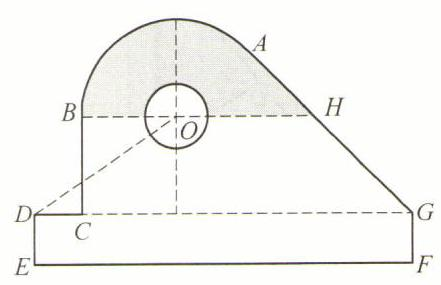
\includegraphics[width=0.3\textwidth]{bodyxb/src/bo_d1ig044601uc738hj6v0_36_1069_930_441_285_0.jpg}
\end{center}

第 1 题图

2. 折扇是我国传统文化的延续, 在我国已有四千年左右的历史,“扇”与“善”谐音,折扇也寓意“善良”“善行”,它常以字画的形式体现我国的传统文化,也是运筹帷幄、决胜千里、大智大勇的象征. 如图为其结构简化图,设扇面 $A$ 、 $B$ 间的圆弧长为 $l,{AB}$ 间的弦长为 $d$ ,圆弧所对的圆心角为 $\theta (\theta$ 为弧度角),则 $l$ 、 $d$ 和 $\theta$ 所满足的恒等关系为 (   ).

\begin{center}
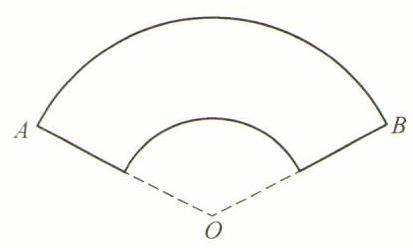
\includegraphics[width=0.3\textwidth]{bodyxb/src/bo_d1ig044601uc738hj6v0_36_1098_1355_413_248_0.jpg}
\end{center}

第 2 题图

A. $\dfrac{2\sin \dfrac{\theta }{2}}{\theta } = \dfrac{d}{l}$ B. $\dfrac{\sin \dfrac{\theta }{2}}{\theta } = \dfrac{d}{l}$

C. $\dfrac{\cos \dfrac{\theta }{2}}{\theta } = \dfrac{d}{l}$ D. $\dfrac{2\cos \dfrac{\theta }{2}}{\theta } = \dfrac{d}{l}$

3. 《九章算术》是中国古代第一部数学著作,成于公元一世纪左右,系统总结了战国、秦、汉时期的数学成就,其中《方田》一章中记载了计算弧田(弧田就是由圆弧和其所对弦所围成的

弓形)的面积所用的经验公式:弧田面积 $= \dfrac{1}{2}$ (弦 $\times$ 矢+矢 $\times$ 矢),公式中“弦”指圆弧所对弦长,“矢”等于半径长与圆心到弦的距离之差,按照上述经验公式计算所得弧田面积与其实际面积之间存在误差,现有圆心角为 $\dfrac{2\pi }{3}$ ,弦长为 ${40}\sqrt{3}$ 米的弧田,其实际面积与按照上述经验公式计算出弧田的面积之间的误差为\blkda{}平方米 (其中 $\pi  \approx  3,\sqrt{3} \approx  {1.73}$ ).

4. 矩形纸片 ${ABCD}$ 中, ${AB} = {10}{{cm}}$ , ${BC} = 8{{cm}}$ ,将其按图 1 的方法分割,并按图 2 的方法焊接成扇形；按图 3 的方法将宽 ${BC}$ 2 等分,把图 3 中的每个小矩形按图 1 分割并把 4 个小扇形焊接成一个大扇形；按图 4 的方法将宽 ${BC}$ 3 等分,把图 4 中的每个小矩形按图 1 分割并把 6 个小扇形焊接成一个大扇形；······；依次将宽 ${BCn}$ 等分,每个小矩形按图 1 分割并把 ${2n}$ 个小扇形焊接成一个大扇形,当 $n \rightarrow  \infty$ 时,最后拼成的大扇形的圆心角的大小为 (   ).

\begin{center}
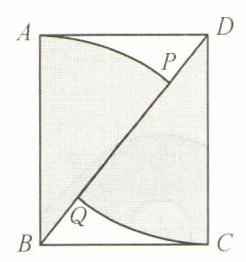
\includegraphics[width=0.2\textwidth]{bodyxb/src/bo_d1ig044601uc738hj6v0_37_254_817_246_262_0.jpg}
\end{center}

第 4 题图 1

\begin{center}
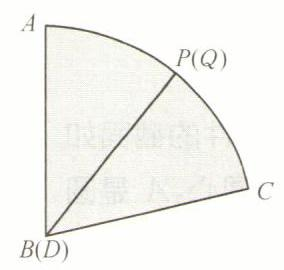
\includegraphics[width=0.2\textwidth]{bodyxb/src/bo_d1ig044601uc738hj6v0_37_552_810_284_270_0.jpg}
\end{center}

第 4 题图 2

\begin{center}
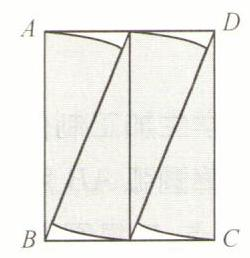
\includegraphics[width=0.2\textwidth]{bodyxb/src/bo_d1ig044601uc738hj6v0_37_889_819_250_258_0.jpg}
\end{center}

第 4 题图 3

\begin{center}
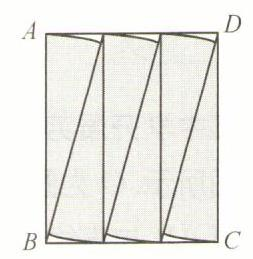
\includegraphics[width=0.2\textwidth]{bodyxb/src/bo_d1ig044601uc738hj6v0_37_1191_815_253_259_0.jpg}
\end{center}

第 4 题图 4

A. 小于 $\dfrac{\pi }{2}$ B. 等于 $\dfrac{\pi }{2}$ C. 大于 $\dfrac{\pi }{2}$ D. 大于 1.6

5. 如图,某住宅小区的平面图呈圆心角为 ${120}^{ \circ  }$ 的扇形 ${AOB}$ , 小区的两个出入口设置在点 $A$ 及点 $C$ 处,且小区里有一条平行于 ${BO}$ 的小路 ${CD}$ ,已知某人从 $C$ 沿 ${CD}$ 走到 $D$ 用了 10 分钟,从 $D$ 沿 ${DA}$ 走到 $A$ 用了 6 分钟,若此人步行的速度为每分钟 50 米,则该扇形的半径 ${OA}$ 的长约为\blkda{}(精确到 1 米).

\begin{center}
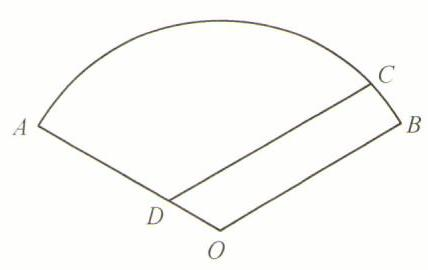
\includegraphics[width=0.3\textwidth]{bodyxb/src/bo_d1ig044601uc738hj6v0_37_1069_1264_428_270_0.jpg}
\end{center}

第 5 题图

\subsection*{20 任意角的三角比}

\subsubsection*{知识点睛}

1. 角的终边与单位圆的交点横坐标为角的余弦、纵坐标为角的正弦,这部分可以结合极坐标知识理解, 也可以结合解析几何章节圆的参数方程对照理解.

2. 角的终边具有对称、垂直等特殊位置关系时,三角比也具有特殊关系,深入研究就是诱导公式.

3. 注意正余弦的有界性,即取值范围是 $\left\lbrack  {-1,1}\right\rbrack$ ,这经常是一些题目的切入点.

4. 同角三角比之间的转化需要熟练掌握,在整理等式与不等式时,“同名”“同角”“同幂”是我们整理的方向.

\subsubsection*{经典习题}

1. 在平面上,已知定点 $A\left( {\sqrt{2},0}\right)$ ,动点 $P\left( {\sin \alpha ,\cos \alpha }\right)$ ,当 $\alpha$ 在区间 $\left\lbrack  {-\dfrac{\pi }{4},\dfrac{\pi }{4}}\right\rbrack$ 上变化时,动线段 ${AP}$ 所形成图形的面积为(   ).

A. $1 + \dfrac{\pi }{4}$ B. $1 - \dfrac{\pi }{4}$ C. $\sqrt{2}$ D. $\dfrac{\pi }{4}$

2. 若 $k$ 是正整数,且 $1 \leq  k \leq  {2022}$ ,则满足方程 $\sin {1}^{ \circ  } + \sin {2}^{ \circ  } + \cdots  + \sin {k}^{ \circ  } = \sin {1}^{ \circ  } \cdot  \sin {2}^{ \circ  } \cdot  \cdots  \cdot$  $\sin {k}^{ \circ  }$ 的 $k$ 有\blkda{}个.

3. 设点 $A$ 的坐标为 $\left( {a,b}\right) ,O$ 是坐标原点,点 $A$ 绕着 $O$ 点顺时针旋转 $\theta$ 后得到 ${A}^{\prime }$ ,则 ${A}^{\prime }$ 的坐标为 (   ).

A. $\left( {a\cos \theta  - b\sin \theta ,a\sin \theta  + b\cos \theta }\right)$

B. $\left( {a\cos \theta  + b\sin \theta ,b\cos \theta  - a\sin \theta }\right)$

C. $\left( {a\sin \theta  + b\cos \theta ,a\cos \theta  - b\sin \theta }\right)$

D. $\left( {b\cos \theta  - a\sin \theta ,b\sin \theta  + a\cos \theta }\right)$

4. 在角 ${\theta }_{1},{\theta }_{2},{\theta }_{3},\cdots ,{\theta }_{29}$ 的终边上分别有一点 ${P}_{1},{P}_{2},{P}_{3},\cdots ,{P}_{29}$ ,如果点 ${P}_{k}$ 的坐标为 $\left( {\sin \left( {{15}^{ \circ  } - {k}^{ \circ  }}\right) ,\sin \left( {{75}^{ \circ  } + {k}^{ \circ  }}\right) }\right) ,1 \leq  k \leq  {29},k \in  \mathbf{N}$ ,则 $\cos {\theta }_{1} + \cos {\theta }_{2} + \cos {\theta }_{3} + \cdots  +$  $\cos {\theta }_{29} =$ \blkda{}.

5. 已知 $\theta  > 0$ ,存在实数 $\varphi$ ,使得对任意 $n \in  {\mathbf{N}}^{ * }$ ,总成立 $\cos \left( {{n\theta } + \varphi }\right)  < \cos \dfrac{\pi }{8}$ ,则 $\theta$ 的最小值是\blkda{}.

6. 实数 $x$ 、 $y$ 满足 $\left\{  {\begin{array}{l} {x}^{2} + \sin y = 3, \\  \sqrt{2}x + \cos y = 2, \end{array}0 \leq  y \leq  \dfrac{\pi }{2}}\right.$ ,则 ${xy} =$ \blkda{}.

7. 已知 ${\alpha }_{1},{\alpha }_{2} \in  \mathbf{R}$ ,且满足等式 $\dfrac{1}{2 + \sin {\alpha }_{1}} + \dfrac{1}{2 + \sin 2{\alpha }_{2}} = 2$ ,则 $\left| {{10\pi } - {\alpha }_{1} - {\alpha }_{2}}\right|$ 的最小值为\blkda{}.

8. " ${\sin }^{2017}\theta  - {\left( 2 - \cos \varphi \right) }^{2018} \geq  0$ " 是 " $\sin \theta \cos \varphi  \geq  1$ " 的(   )条件.

A. 充分不必要 B. 必要不充分

C. 充要 D. 既不充分也不必要

9. 若 ${\sin }^{2018}\alpha  - {\left( 2 - \cos \beta \right) }^{1009} \geq  \left( {3 - \cos \beta  - {\cos }^{2}\alpha }\right) \left( {1 - \cos \beta  + {\cos }^{2}\alpha }\right)$ ,则 $\sin \left( {\alpha  + \dfrac{\beta }{2}}\right)  =$ \blkda{}.

\subsection*{21 三角恒等式}

\subsubsection*{知识点睛}

1. 化简时注意结合角的范围判断符号.

2. 由三角比求角,已知条件中的范围相对宽泛,需要结合中间过程中三角比的符号精确角的范围.

3. 二倍角余弦的公式及变形要重点掌握.

4. 辅助角公式是两角和差的正余弦公式的逆应用.

5. 万能公式确实是万能的, 在个别时候计算量并不大, 是很好的工具.

6. 半角正切公式 $\tan \dfrac{\theta }{2} = \dfrac{\sin \theta }{1 + \cos \theta }$ 经常有出其不意的效果.

\subsubsection*{经典习题}

1. 已知 $\sin \alpha  + \sin \beta  = \sin \left( {\alpha  + \beta }\right)$ ,有以下两个结论:

① 存在 $\alpha$ 终边在第一象限, $\beta$ 终边在第二象限;

② 存在 $\alpha$ 终边在第一象限, $\beta$ 终边在第四象限.

下列说法中正确的是(   ).

A. ①②均正确 B. ①②均错误

C. ①错误, ②正确 D. ①正确, ②错误

2. 已知 $x \geq  y \geq  z \geq  \dfrac{\pi }{8}$ ,又 $x + y + z = \dfrac{3\pi }{4}$ ,则 $\cos x \cdot  \sin y \cdot  \cos z$ 的最大值为\blkda{}.

3. 已知椭圆 $\dfrac{{x}^{2}}{{a}^{2}} + \dfrac{{y}^{2}}{{b}^{2}} = 1\left( {a > b > 0}\right)$ 中 $a$ 、 $b$ 、 $c$ 成等比数列, $A$ 、 $B$ 是椭圆的左、右顶点, $P$ 是椭圆上不同于 $A\text{ 、 }B$ 的一点,直线 ${PA}\text{ 、 }{PB}$ 倾斜角分别为 $\alpha \text{ 、 }\beta$ ,则 $\dfrac{\cos \left( {\alpha  - \beta }\right) }{\cos \left( {\alpha  + \beta }\right) } =$ \blkda{}.

4. 在 $\bigtriangleup  {ABC}$ 中, ${AC} = 2,\dfrac{2}{\tan A} + \dfrac{1}{\tan B} = 1$ ,若 $\bigtriangleup  {ABC}$ 的面积为 2,则 ${AB} =$ \blkda{}.

5. 已知 $\sin \alpha  + \cos \beta  = \dfrac{3}{5},\cos \alpha  + \sin \beta  = \dfrac{4}{5}$ ,则 $\cos \alpha \sin \beta$ 的值为 (   ).

A. $- \dfrac{11}{100}$ B. $- \dfrac{13}{100}$ C. $- \dfrac{15}{100}$ D. $- \dfrac{17}{100}$

6. 有一道填空题, 由于一些原因造成横线上的内容缺失了, 现已知结论, 请在横线上填写原题的一个条件, 题目如下:

已知 $\alpha$ 、 $\beta$ 均为锐角,且 $\sin \alpha  - \sin \beta  =  - \dfrac{1}{2}$ ,\blkda{},则 $\cos \left( {\alpha  - \beta }\right)  = \dfrac{59}{72}$ .

7. 设锐角 $\bigtriangleup {ABC}$ 内部的一点 $O$ 满足 $\left| {OA}\right|  = \left| {OB}\right|  = \left| {OC}\right|$ ,且 $\dfrac{1}{2\cos A} \cdot  \vv{OA} + \dfrac{\cos B}{\sin C} \cdot  \vv{AB} +$  $\dfrac{\cos C}{\sin B} \cdot  \vv{AC} = \vv{0}$ ,则角 $A$ 的大小可能为 (   ).

A. $\dfrac{\pi }{4}$ B. $\dfrac{\pi }{6}$ C. $\dfrac{\pi }{3}$ D. $\dfrac{5\pi }{12}$

8. 提鞋公式也叫李善兰辅助角公式, 其正弦型如下:

$
a\sin x + b\cos x = \sqrt{{a}^{2} + {b}^{2}}\sin \left( {x + \varphi }\right) , - \pi  < \varphi  \leq  \pi .
$

下列判断中错误的是(   ).

A. 当 $a > 0,b > 0$ 时,辅助角 $\varphi  = \arctan \dfrac{b}{a}$

B. 当 $a > 0,b < 0$ 时,辅助角 $\varphi  = \arctan \dfrac{b}{a} + \pi$

C. 当 $a < 0,b > 0$ 时,辅助角 $\varphi  = \arctan \dfrac{b}{a} + \pi$

D. 当 $a < 0,b < 0$ 时,辅助角 $\varphi  = \arctan \dfrac{b}{a} - \pi$

9. 已知函数 $y = a\sin x + \cos x,x \in  \left\lbrack  {0,\dfrac{\pi }{2}}\right\rbrack$ ,其最小值为 $a$ ,则实数 $a$ 的取值范围是\blkda{}.

\subsubsection*{知识点睛}

1. 在 $\bigtriangleup {ABC}$ 中, $A + B + C = \pi$ ,则 $\sin \left( {A + B}\right)  = \sin C,\cos \left( {A + B}\right)  =  - \cos C$ ,正弦全正.

2. 三角形三边性质:两边之和大于第三边,两边之差小于第三边,等价于三角形内角余弦值范围为 $\left\lbrack  {-1,1}\right\rbrack$ .

3. 三角形为钝角三角形,需要最大角余弦为负；三角形为锐角三角形,需要最大角余弦为正, 若不知道哪个角最大, 则需要三个角的余弦均为正.

4. 除了常用的三角形面积公式, 还建议大家了解:

① $S = \sqrt{p \cdot  \left( {p - a}\right)  \cdot  \left( {p - b}\right)  \cdot  \left( {p - c}\right) }$ ,其中 $p = \dfrac{a + b + c}{2}$ ；

② $S = \dfrac{1}{2}\sqrt{{\left| \vv{AB}\right| }^{2} \cdot  {\left| \vv{AC}\right| }^{2} - {\left( \vv{AB} \cdot  \vv{AC}\right) }^{2}}$ .

\subsubsection*{经典习题}

1. 已知 $O$ 为锐角 $\bigtriangleup {ABC}$ 的外心, $O$ 到三边 $a\text{ 、 }b\text{ 、 }c$ 的距离分别为 $k\text{ 、 }m\text{ 、 }n$ ,则 (   ).

A. $k : m : n = a : b : c$ B. $k : m : n = \dfrac{1}{a} : \dfrac{1}{b} : \dfrac{1}{c}$

C. $k : m : n = \tan A : \tan B : \tan C$ D. $k : m : n = \cos A : \cos B : \cos C$

2. 设 $\bigtriangleup {ABC}$ 的内角 $A\text{ 、 }B\text{ 、 }C$ 所对的边分别为 $a\text{ 、 }b\text{ 、 }c$ ,且 $A - C = \dfrac{\pi }{2}$ . 若 $a,b,c$ 成等差数列, 则 $\cos B =$ \blkda{}.

3. 在 $\bigtriangleup  {ABC}$ 中,若 $\dfrac{b}{a} + \dfrac{a}{b} = 4\cos C,\cos \left( {A - B}\right)  = \dfrac{1}{6}$ ,则 $\cos C =$ \blkda{}.

4. 在 $\bigtriangleup {ABC}$ 中, $A\text{ 、 }B\text{ 、 }C$ 所对的边分别为 $a\text{ 、 }b\text{ 、 }c$ ,现有下列五个命题:

① 若 $\tan A \geq  \tan B$ ,则 $\sin A \geq  \sin B$ ；

② 若 $a + b > {2c}$ ,则 $C < \dfrac{\pi }{3}$ ；

③ 若 $\dfrac{a}{\cos B} = \dfrac{b}{\cos A}$ ,则 $\bigtriangleup  {ABC}$ 为等腰三角形；

④ 若 $\sin A < \cos B$ ,则 $\bigtriangleup  {ABC}$ 为钝角三角形；

⑤ 若 $\tan A\tan B > 1$ ,则 $\tan A\tan B\tan C > 1$ .

其中,正确命题的序号是\blkda{}.

5. 在 $\bigtriangleup {ABC}$ 中, $A = {60}^{ \circ  },b = 1$ ,其面积为 $\sqrt{3}$ ,则 $\dfrac{a + b + c}{\sin A + \sin B + \sin C} =$ \blkda{}.

6. 已知 $\bigtriangleup {ABC}$ 的三边分别为 $a\text{ 、 }b\text{ 、 }c$ ,所对的角分别为 $A\text{ 、 }B\text{ 、 }C$ ,且满足 $\dfrac{1}{a + b} + \dfrac{1}{b + c} =$  $\dfrac{3}{a + b + c}$ ,且 $\bigtriangleup {ABC}$ 的外接圆的面积为 ${3\pi }$ ,则 $f\left( x\right)  = \cos {2x} + 4\left( {a + c}\right) \sin x + 1$ 的最大值的取值范围为\blkda{}.

7. 设 $\bigtriangleup {ABC}$ 的内角 $A\text{ 、 }B\text{ 、 }C$ 所对的边长分别为 $a\text{ 、 }b\text{ 、 }c$ ,则下列命题:

① 若 ${ab} > {c}^{2}$ ,则 $C < \dfrac{\pi }{3}$ ；

② 若 $\tan A \leq  \tan B$ ,则 $\sin A \leq  \sin B$ ；

③ 若 $\sin A < \cos B$ ,则 $\bigtriangleup  {ABC}$ 为钝角三角形；

④ 若 $\tan A \cdot  \tan B > 1$ ,则 $\tan A \cdot  \tan B \cdot  \tan C > 2$ .

其中,真命题的个数是(   ).

A. 1 B. 2 C. 3 D. 4

8. 在 $\bigtriangleup {ABC}$ 中,角 $A\text{ 、 }B\text{ 、 }C$ 所对的边分别为 $a\text{ 、 }b\text{ 、 }c,a = 2,2\sin A = \sin C$ . 若 $B$ 为钝角, $\cos {2C} =  - \dfrac{1}{4}$ ,则 $\bigtriangleup  {ABC}$ 的面积为\blkda{}.

9. 在 $\bigtriangleup {ABC}$ 中,角 $A\text{ 、 }B\text{ 、 }C$ 所对边的长分别为 $a\text{ 、 }b\text{ 、 }c$ ,现有下列四个结论:

① 若 $a = \sqrt{2},b = 2\sqrt{2}$ ,则 $A$ 可以是 $\dfrac{\pi }{3}$ ;

② 若 $A = \dfrac{\pi }{6},a = 1,c = \sqrt{3}$ ,则 $b$ 只能是 1 ；

③ 若 $\bigtriangleup {ABC}$ 是锐角三角形, $a = 2,b = 3$ ,则边长 $c$ 的取值范围是 $\left( {\sqrt{5},\sqrt{13}}\right)$ ;

④ 若 ${\sin }^{2}A \leq  {\sin }^{2}B + {\sin }^{2}C - \sin B\sin C$ ,则角 $A$ 的取值范围是 $\left( {0,\dfrac{\pi }{3}}\right\rbrack$ .

其中,正确结论的序号是\blkda{}.

10. 对于 $\bigtriangleup {ABC}$ ,若存在 $\bigtriangleup {A}_{1}{B}_{1}{C}_{1}$ ,满足 $\dfrac{\cos A}{\sin {A}_{1}} = \dfrac{\cos B}{\sin {B}_{1}} = \dfrac{\cos C}{\sin {C}_{1}} = 1$ ,则称 $\bigtriangleup {ABC}$ 为 “ $V$ 类三角形”,“ $V$ 类三角形”一定满足有一个内角为(   ).

A. ${30}^{ \circ  }$ B. ${45}^{ \circ  }$ C. 60° D. ${75}^{ \circ  }$

\subsection*{23 三角函数的性质}

\subsubsection*{知识点睛}

1. 三角函数为 “多对一” 型函数, 相同的值域会有不同的定义域, 计算结果需要注意是否漏解.

2. 处理 $f\left( x\right)  = A\sin \left( {{\omega x} + \varphi }\right)$ 型函数时,可将它当作复合函数,设 ${\omega x} + \varphi  = \theta$ ,研究 $y =$  $A\sin \theta$ 的性质. 其中单调性问题注意“同增异减”.

3. 在 $f\left( x\right)  = A\sin \left( {{\omega x} + \varphi }\right)$ 模型中, $\omega$ 的求解经常和周期相关.

4. 处理 $f\left( x\right)  = A\sin \left( {{\omega x} + \varphi }\right)$ 型函数时,其奇偶性可以根据函数性质快速求解,如果是奇函数, $f\left( 0\right)  = 0$ ; 如果是偶函数, $f\left( 0\right)  =  \pm  A$ .

\subsubsection*{经典习题}

1. 若函数 $y = \tan \left( {\omega x}\right)$ 在 $\left\lbrack  {-\dfrac{\pi }{4},\dfrac{\pi }{4}}\right\rbrack$ 上为严格减函数,则实数 $\omega$ 的取值范围是\blkda{}.

2. 已知函数 $f\left( x\right)  = {\sin }^{2}\dfrac{\omega x}{2} + \dfrac{\sqrt{3}}{2}\sin {\omega x} - \dfrac{1}{2}\left( {\omega  > 0}\right) ,x \in  \mathbf{R}$ ,若 $f\left( x\right)$ 在区间 $\left( {\pi ,{2\pi }}\right)$ 内没有零点,则 $\omega$ 的取值范围是\blkda{}.

3. 设函数 $f\left( x\right)  = {\sin }^{4}\dfrac{kx}{10} + {\cos }^{4}\dfrac{kx}{10}$ ,其中 $k$ 是一个正整数,若对任意实数 $a$ ,均有 $\{ f\left( x\right)  \mid  a <$  $x < a + 1\}  = \{ f\left( x\right)  \mid  x \in  \mathbf{R}\}$ ,则 $k$ 的最小值为\blkda{}.

4. 函数 $y = \cos \left( {\dfrac{\pi }{2}\left( {x + \varphi }\right) }\right) ,0 < \varphi  < \pi$ 是奇函数,那么常数 $\varphi$ 的最大值为\blkda{}.

5. 设 $a,b \in  \mathbf{R}$ ,若存在区间 $\left\lbrack  {a,b}\right\rbrack$ 使得函数 $f\left( x\right)  = \sin x - \dfrac{1}{2}$ 在此区间上仅有两个零点,则 $b - a$ 的取值范围是\blkda{}.

6. 方程 $2\cos {2x} \cdot  \left( {\cos {2x} - \cos \dfrac{{2020}{\pi }^{2}}{x}}\right)  =  - 1 + \cos {4x}$ 的所有正数解之和为(   ).

A. ${825\pi }$ B. ${1011\pi }$ C. ${1836\pi }$ D. ${2020\pi }$

7. 若 $x\text{ 、 }y \in  \left\lbrack  {-\dfrac{\pi }{4},\dfrac{\pi }{4}}\right\rbrack  ,a \in  \mathbf{R}$ ,且 $\left\{  \begin{array}{l} {x}^{3} + \sin x - {2a} = 0, \\  8{y}^{3} + \sin {2y} + {2a} = 0, \end{array}\right.$ 则 $\sin \left( {x + {2y}}\right)  =$ \blkda{}.

8. 已知 $f\left( x\right)  = \tan x$ ,若存在 $\alpha ,\beta  \in  \left( {0,\dfrac{\pi }{2}}\right)$ ,使得 $f\left( \alpha \right)  - f\left( \beta \right)  = 2$ ,则 $\alpha  - \beta$ (   ).

A. 有最大值, 有最小值 B. 有最大值, 无最小值

C. 无最大值, 有最小值 D. 无最大值, 无最小值

9. 函数 $y = {\sin }^{2}x + 2\cos x$ 的定义域为 $\left\lbrack  {-\dfrac{2\pi }{3},\alpha }\right\rbrack$ ,值域为 $\left\lbrack  {-\dfrac{1}{4},2}\right\rbrack$ ,则 $\alpha$ 的取值范围是\blkda{}.

10. 若 $\omega  > 0$ ,函数 $f\left( x\right)  = 3\sin {\omega x} + 4\cos {\omega x}\left( {0 \leq  x \leq  \dfrac{\pi }{3}}\right)$ 的值域为 $\left\lbrack  {4,5}\right\rbrack$ ,则 $\cos \left( {\dfrac{\pi }{3}\omega }\right)$ 的取值范围是\blkda{}.

11. 设函数 $f\left( x\right)  = \sin \left( {x - \dfrac{\pi }{6}}\right)$ ,若对于任意 $\alpha  \in  \left\lbrack  {-\dfrac{5\pi }{6}, - \dfrac{\pi }{2}}\right\rbrack$ ,在区间 $\left\lbrack  {0,m}\right\rbrack$ 上总存在唯一确定的 $\beta$ ,使得 $f\left( \alpha \right)  + f\left( \beta \right)  = 0$ ,则 $m$ 的最小值为 (   ).

A. $\dfrac{\pi }{6}$ B. $\dfrac{\pi }{2}$ C. $\dfrac{7\pi }{6}$ D. $\pi$

12. 函数 $f\left( x\right)  = \sin {\omega x}\left( {\omega  > 0}\right)$ 的图象与其对称轴在 $y$ 轴右侧的交点从左到右依次记为 ${A}_{1}$ , ${A}_{2},{A}_{3},\cdots ,{A}_{n},\cdots$ ,在点列 $\left\{  {A}_{n}\right\}$ 中存在三个不同的点 ${A}_{k}\text{ 、 }{A}_{i}\text{ 、 }{A}_{p}$ ,使得 $\bigtriangleup {A}_{k}{A}_{i}{A}_{p}$ 是等腰直角三角形,将满足上述条件的 $\omega$ 值从小到大组成的数列记为 $\left\{  {\omega }_{n}\right\}$ ,则 ${\omega }_{2019} =$ \blkda{}.

13. 已知函数 $f\left( x\right)  = \sin {\omega x}\left( {\omega  > 0}\right)$ ,将 $f\left( x\right)$ 的图象向左平移 $\dfrac{\pi }{2\omega }$ 个单位得到函数 $g\left( x\right)$ 的图象,令 $h\left( x\right)  = f\left( x\right)  + g\left( x\right)$ ,如果存在实数 $m$ ,使得对任意的实数 $x$ ,都有 $h\left( m\right)  \leq  h\left( x\right)  \leq$  $h\left( {m + 1}\right)$ 成立,那么 $\omega$ 的最小值为\blkda{}.

14. 已知函数 $f\left( x\right)  = \sin \left( {{\omega x} + \varphi }\right) \left( {\omega  > 0,0 \leq  \varphi  \leq  {2\pi }}\right)$ 是 $\mathbf{R}$ 上的偶函数,图象关于点 $M\left( {\dfrac{3}{4}\pi ,0}\right)$ 对称,在 $\left\lbrack  {0,\dfrac{\pi }{2}}\right\rbrack$ 是单调函数,则符合条件的数组 $\left( {\omega ,\varphi }\right)$ 有\blkda{} 对.

15. 已知函数 $f\left( x\right)  = \left| {{\sin }^{2}x - \sqrt{3}\cos x\cos \left( {\dfrac{3\pi }{2} - x}\right)  - \dfrac{1}{2}}\right|$ ,若将函数 $y = f\left( x\right)$ 的图象向左平移 $a$ 个单位 $\left( {0 < a < \pi }\right)$ ,所得图象关于 $y$ 轴对称,则实数 $a$ 的取值集合为\blkda{}.

\section*{向量}

向量是非常好用的工具, 在解析几何与立体几何中, 向量可以弥补对图形想象力较弱的缺陷,少添甚至不添辅助线,就能解决问题. 在高考数学中,向量不仅在解答题中经常为其他知识点搭桥铺路,而且由于向量有三种表示(符号表示、几何表示、坐标表示),并处于函数和几何的交汇处,涉及数形结合,所以向量也是填选压轴题中非常常见且重要的考点.

\subsection*{24 向量的几何意义:投影}

\subsubsection*{知识点睛}

向量数量积的几何意义是一个向量在另一个向量方向上的数量投影与另一个向量的模的乘积,注意 $\vv{a}$ 在 $\vv{b}$ 方向上的投影向量为 $\dfrac{\vv{a} \cdot  \vv{b}}{{|\vv{b}| }^{2}} \cdot  \vv{b}$ ,其实质为投影数量与单位向量的数乘. 在考查中,我们常常容易搞混两者,解题时要注意是谁在谁上的投影,而不能颠倒顺序. (注:上海教材中特意在投影上区分了“数量投影”和“投影向量”,我们在压轴题的应用中主要用的是向量的“数量投影”)

\subsubsection*{经典习题}

1. 如图,已知 $M\text{ 、 }N$ 在以 ${AB}$ 为直径的圆上,若 ${AB} = 5,{AM} =$ 3, ${BN} = 2$ ,则 $\vv{AB} \cdot  \vv{MN} =$ \blkda{}.

\begin{center}
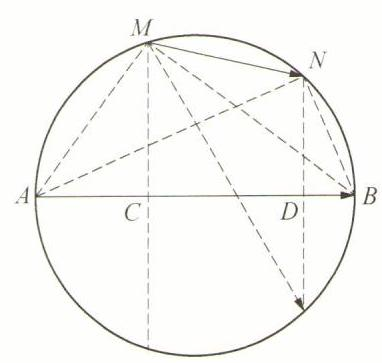
\includegraphics[width=0.3\textwidth]{bodyxb/src/bo_d1ig044601uc738hj6v0_47_1124_1081_382_363_0.jpg}
\end{center}

第 1 题图

2. 在平面直角坐标系 ${xOy}$ 中,起点为坐标原点的向量 $\vv{a}$ 、 $\vv{b}$ 满足 $\left| \vv{a}\right|  = |\vv{b}|  = 1$ ,且 $\vv{a} \cdot  \vv{b} =  - \dfrac{1}{2},\vv{c} = \left( {m,1 - m}\right) ,\vv{d} = (n$ , $1 - n)\left( {m,n \in  \mathbf{R}}\right)$ ,若存在向量 $\vv{a}\text{ 、 }\vv{b}$ ,对于任意实数 $m\text{ 、 }n$ ,不等式 $\left| {\vv{a} - \vv{c}}\right|  + \left| {\vv{b} - \vv{d}}\right|  \geq  T$ 成立,则实数 $T$ 的最大值为\blkda{}.

3. 如图,已知半圆 $O$ 的直径 ${AB} = 4,\bigtriangleup {OAC}$ 是等边三角形,若点 $P$ 是边 ${AC}$ (包含端点 $A\text{ 、 }C$ ) 上的动点,点 $Q$ 在弧 ${BC}$ 上,且满足 ${OQ} \bot  {OP}$ ,则 $\vv{OP} \cdot  \vv{BQ}$ 的最小值为\blkda{}.

\begin{center}
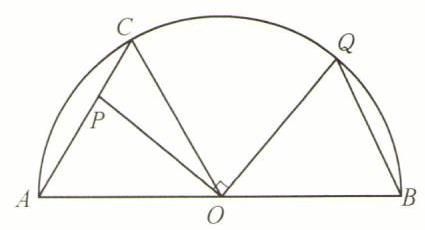
\includegraphics[width=0.3\textwidth]{bodyxb/src/bo_d1ig044601uc738hj6v0_47_616_1711_425_230_0.jpg}
\end{center}

第 3 题图

4. 如图,若同一平面上的四边形 ${PQRS}$ 满足: ${mn}\vv{RP} =$  $n\left( {1 - {3m}}\right) \vv{QP} + m\left( {n - 1}\right) \vv{SP}\left( {m > 0,n > 0}\right)$ ,则当 $\bigtriangleup {PRS}$ 的面积是 $\bigtriangleup {PQR}$ 的面积的 $\dfrac{1}{3}$ 时, $\dfrac{1}{m + n}$ 的最大值为\blkda{}.

\begin{center}
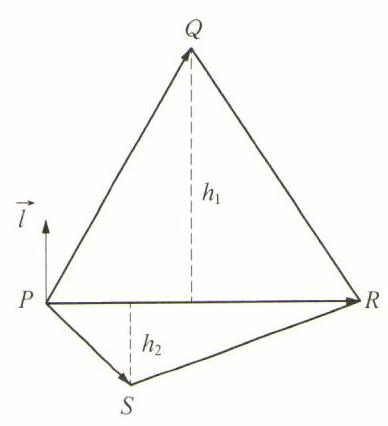
\includegraphics[width=0.3\textwidth]{bodyxb/src/bo_d1ig044601uc738hj6v0_48_1115_124_388_426_0.jpg}
\end{center}

第 4 题图

5. 已知向量 $\vv{a}$ 与 $\vv{b}$ 的夹角为 ${60}^{ \circ  }$ ,且 $|\vv{b}|  = 2\left| \vv{a}\right|  = 2$ ,若 $\vv{c} = \lambda \vv{a} +$  $\mu \vv{b}$ ,其中 $\lambda  + {2\mu } = 2$ ,则向量 $\vv{a}$ 在 $\vv{c}$ 上的投影的取值范围为\blkda{}.

6. 在边长为 1 的正六边形 ${ABCDEF}$ 中,记以 $A$ 为起点,其余顶点为终点的向量分别为 $\vv{{a}_{1}}\text{ 、 }\vv{{a}_{2}}\text{ 、 }\vv{{a}_{3}}\text{ 、 }\vv{{a}_{4}}\text{ 、 }\vv{{a}_{5}}$ ,若 $\vv{{a}_{i}}$ 与 $\vv{{a}_{j}}$ 的夹角记为 ${\theta }_{ij}$ ,其中 $i\text{ 、 }j \in  \{ 1,2,3,4,5\}$ ,且 $i \neq  j$ ,则 $\left| \vv{{a}_{i}}\right|  \cdot  \cos {\theta }_{ij}$ 的最大值为\blkda{}.

7. 已知 ${AB}$ 为单位圆 $O$ 的一条弦, $P$ 为单位圆 $O$ 上的点,若 $f\left( \lambda \right)  = \left| {\vv{AP} - \lambda \vv{AB}}\right| \left( {\lambda  \in  \mathbf{R}}\right)$ 的最小值为 $m$ ,当点 $P$ 在单位圆上运动时, $m$ 的最大值为 $\dfrac{4}{3}$ ,则线段 ${AB}$ 长度为\blkda{}.

8. 如图所示的同心圆中,大、小圆的半径分别为 2 和 1,点 $P$ 在大圆上, ${PA}$ 与小圆相切于点 $A,Q$ 为小圆上的点,则 $\vv{PA} \cdot  \vv{PQ}$ 的取值范围是\blkda{}.

\begin{center}
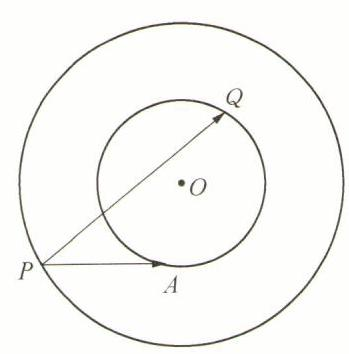
\includegraphics[width=0.2\textwidth]{bodyxb/src/bo_d1ig044601uc738hj6v0_48_1154_911_349_354_0.jpg}
\end{center}

第 8 题图

\subsection*{25 向量“三化”原则}

\subsubsection*{知识点睛}

1. “三化”原则指的是“特殊化”“坐标化”“模的问题平方化”. 由于向量可以任意平移,所以可以以某一个向量作为 $x$ 轴进行建系处理.

2. 求模问题一般转化为求模的平方,与向量数量积联系,并灵活应用 ${\vv{a}}^{2} = {\left| \vv{a}\right| }^{2}$ ,注意勿忘记开方.

3. $\vv{a} \cdot  \vv{a} = {\vv{a}}^{2} = {\left| \vv{a}\right| }^{2}$ 或 $\left| \vv{a}\right|  = \sqrt{{\vv{a}}^{2}}$ ,此性质可用来求向量的模,实现实数运算与向量运算的相互转化.

\subsubsection*{经典习题}

1. 已知 $x\text{ 、 }y$ 是正实数, $\bigtriangleup {ABC}$ 的三边长为 ${CA} = 3,{CB} = 4,{AB} = 5$ ,点 $P$ 是边 ${AB}$ ( $P$ 与点 $A\text{ 、 }B$ 不重合) 上任一点,且 $\vv{CP} = x \cdot  \dfrac{\vv{CA}}{\left| \vv{CA}\right| } + y$ . $\dfrac{\vv{CB}}{\left| \vv{CB}\right| }$ ,若不等式 ${2x} + {3y} \geq  {mxy}$ 恒成立,则实数 $m$ 的取值范围是 (   ).

\begin{center}
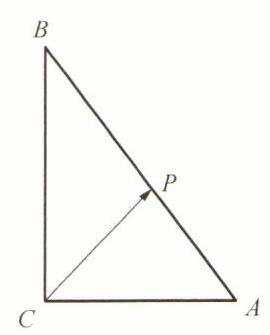
\includegraphics[width=0.2\textwidth]{bodyxb/src/bo_d1ig044601uc738hj6v0_49_1233_1154_270_335_0.jpg}
\end{center}

第 1 题图

A. $m \leq  \dfrac{3}{2} + \sqrt{2}$ B. $m \leq  2\sqrt{6}$

C. $m \leq  \dfrac{3}{2}\sqrt{2}$ D. $m \leq  3$

2. 已知点 $D$ 为圆 $O : {x}^{2} + {y}^{2} = 4$ 的弦 ${MN}$ 的中点,点 $A$ 的坐标为 (1,0),且 $\vv{AM} \cdot  \vv{AN} = 1$ ,则 $\vv{OA} \cdot  \vv{OD}$ 的最大值为\blkda{}.

3. 如图所示,在直角梯形 ${ABCD}$ 中,已知 ${AD}//{BC}$ , $\angle {ABC} =$  $\dfrac{\pi }{2},{AB} = {AD} = 1,{BC} = 2,M$ 为 ${BD}$ 的中点,设 $P\text{ 、 }Q$ 分别为线段 ${AB}\text{ 、 }{CD}$ 上的动点,若 $P\text{ 、 }M\text{ 、 }Q$ 三点共线,则 $\vv{AQ}$ . $\vv{CP}$ 的最大值为\blkda{}.

\begin{center}
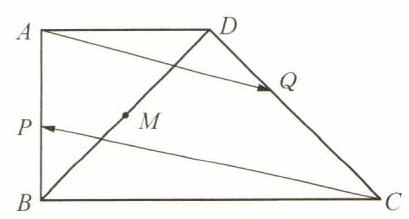
\includegraphics[width=0.3\textwidth]{bodyxb/src/bo_d1ig044601uc738hj6v0_49_1091_1773_409_219_0.jpg}
\end{center}

第 3 题图

4. 在 $\bigtriangleup {ABC}$ 中, ${AB} = 3,{AC} = 2$ ,点 $D$ 在边 ${BC}$ 上,若 $\vv{AB} \cdot  \vv{AD} = 1,\vv{AD} \cdot  \vv{AC} = \dfrac{5}{3}$ ,则 $\vv{AB} \cdot  \vv{AC}$ 的值为\blkda{}.

5. 已知 ${{Rt}} \bigtriangleup  {ABC}$ 中, $\angle A = {90}^{ \circ  },{AB} = 4,{AC} = 6$ ,在三角形所在的平面内有两个动点 $M$ 和 $N$ ,满足 $\left| \vv{AM}\right|  = 2,\vv{MN} = \vv{NC}$ ,则 $\left| \vv{BN}\right|$ 的取值范围是(   ).

\begin{center}
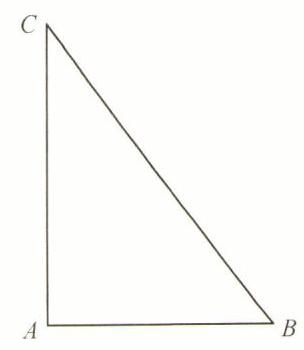
\includegraphics[width=0.2\textwidth]{bodyxb/src/bo_d1ig044601uc738hj6v0_50_1199_285_304_350_0.jpg}
\end{center}

第 5 题图

A. $\left\lbrack  {3\sqrt{2},\sqrt{34}}\right\rbrack$

B. $\left\lbrack  {4,6}\right\rbrack$

C. $\left\lbrack  {2\sqrt{5},4\sqrt{2}}\right\rbrack$

D. $\left\lbrack  {\dfrac{2}{3}\sqrt{{63} - {12}\sqrt{2}},\dfrac{2}{3}\sqrt{{63} + {12}\sqrt{2}}}\right\rbrack$

6. 在 $\bigtriangleup {ABC}$ 中, $\vv{AM} = \dfrac{1}{2}\vv{AB},\vv{AN} = \dfrac{1}{3}\vv{AC},{BN}$ 与 ${CM}$ 交于点 $E,\vv{AB} = \vv{a},\vv{AC} = \vv{b}$ ,则 $\vv{AE} =$ \blkda{}(用 $\vv{a}$ 、 $\vv{b}$ 表示).

7. 已知 $A\text{ 、 }B\text{ 、 }C$ 是单位圆上三个互不相同的点,若 $\left| \vv{AB}\right|  = \left| \vv{AC}\right|$ ,则 $\vv{AB} \cdot  \vv{AC}$ 的最小值是\blkda{}.

8. 已知向量 $\vv{a} = \left( {\cos \alpha ,\sin \alpha }\right) ,\vv{b} = \left( {\cos \beta ,\sin \beta }\right)$ ,且 $\alpha  - \beta  = \dfrac{\pi }{3}$ ,若向量 $\vv{c}$ 满足 $\left| {\vv{c} - \vv{a} - \vv{b}}\right|  =$ 1,则 $\left| \vv{c}\right|$ 的最大值为\blkda{}.

9. 已知平面向量 $\vv{a}$ 、 $\vv{b}$ 满足条件: $\vv{a} \cdot  \vv{b} = 0,\left| \vv{a}\right|  = \cos \alpha ,|\vv{b}|  = \sin \alpha ,\alpha  \in  \left( {0,\dfrac{\pi }{2}}\right)$ ,若向量 $\vv{c} =$  $\lambda \vv{a} + \mu \vv{b}\left( {\lambda ,\mu  \in  \mathbf{R}}\right)$ ,且 ${\left( 2\lambda  - 1\right) }^{2}{\cos }^{2}\alpha  + {\left( 2\mu  - 1\right) }^{2}{\sin }^{2}\alpha  = \dfrac{1}{9}$ ,则 $\left| \vv{c}\right|$ 的最小值为\blkda{}.

10. 正方形 ${ABCD}$ 的边长为 2,对角线 ${AC}\text{ 、 }{BD}$ 相交于点 $O$ ,动点 $P$ 满足 $\left| \vv{OP}\right|  = \dfrac{\sqrt{2}}{2}$ ,若 $\vv{AP} =$  $m\vv{AB} + n\vv{AD}$ ,其中 $m\text{ 、 }n \in  \mathbf{R}$ ,则 $\dfrac{{2m} + 1}{{2n} + 2}$ 的最大值是\blkda{}.

11. $\bigtriangleup {ABC}$ 中, ${BC}$ 边上的中垂线分别交 ${BC}\text{ 、 }{AC}$ 于点 $D\text{ 、 }E$ ,若 $\vv{AE} \cdot  \vv{BC} = 6,\left| \vv{AB}\right|  = 2$ ,则 ${AC} =$ \blkda{}.

12. 已知 $O$ 为矩形 ${P}_{1}{P}_{2}{P}_{3}{P}_{4}$ 内的一点,满足 $O{P}_{1} = 4,O{P}_{3} = 5,{P}_{1}{P}_{3} = 7$ ,则 $\vv{O{P}_{2}} \cdot  \vv{O{P}_{4}}$ 的值为\blkda{}.

13. 在直角三角形 ${ABC}$ 中, $\angle A = \dfrac{\pi }{2},{AB} = 3,{AC} = 4,E$ 为三角形 ${ABC}$ 内一点,且 ${AE} = \dfrac{\sqrt{2}}{2}$ , 若 $\vv{AE} = \lambda \vv{AB} + \mu \vv{AC}$ ,则 ${3\lambda } + {4\mu }$ 的最大值等于\blkda{}.

\subsection*{26 向量极化恒等式}

\subsubsection*{知识点睛}

1. 极化恒等式: $\vv{a} \cdot  \vv{b} = \dfrac{1}{4}\left\lbrack  {{\left( \vv{a} + \vv{b}\right) }^{2} - {\left( \vv{a} - \vv{b}\right) }^{2}}\right\rbrack$ .

2. 极化恒等式的应用主要是为了解决共起点的向量数量积问题.

3. 极化恒等式的三角形模式: 如图,在 $\bigtriangleup {ABC}$ 中,设 $D$ 为 ${BC}$ 的中点,则 $\vv{AB} \cdot  \vv{AC} = {\left| AD\right| }^{2} - {\left| BD\right| }^{2}$ .

\begin{center}
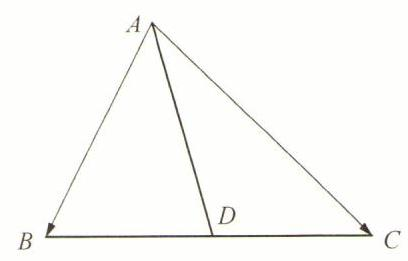
\includegraphics[width=0.3\textwidth]{bodyxb/src/bo_d1ig044601uc738hj6v0_51_1070_753_408_261_0.jpg}
\end{center}

4. 三角形模式是平面向量极化恒等式的终极模式, 以此解决问题很方便.

5. 记忆规律:向量的数量积等于第三边的中线长与第三边长的一半的平方差.

\subsubsection*{经典习题}

1. 已知正方形 ${ABCD}$ 边长为 8, $\vv{BE} = \vv{EC},\vv{DF} = 3\vv{FA}$ ,若在正方形边上恰有 6 个不同的点 $P$ , 使 $\vv{PE} \cdot  \vv{PF} = \lambda$ ,则 $\lambda$ 的取值范围为\blkda{}.

2. 已知 $P$ 是半径为 2,圆心角为 $\dfrac{\pi }{3}$ 的一段圆弧 ${AB}$ 上的一点,若 $\vv{AB} = 2\vv{BC}$ ,则 $\vv{PC} \cdot  \vv{PA}$ 的值域是\blkda{}.

3. 如图,在折线 ${ABCD}$ 中, ${AB} = {BC} = {CD} = 4,\angle {ABC} =$  $\angle {BCD} = {120}^{ \circ  },E\text{ 、 }F$ 分别是 ${AB}\text{ 、 }{CD}$ 的中点,若折线上满足条件 $\vv{PE} \cdot  \vv{PF} = k$ 的点 $P$ 至少有 4 个,则实数 $k$ 的取值范围是\blkda{}.

\begin{center}
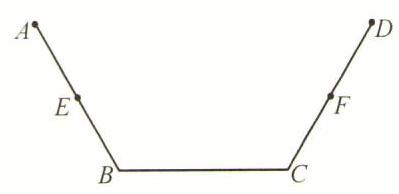
\includegraphics[width=0.3\textwidth]{bodyxb/src/bo_d1ig044601uc738hj6v0_51_1079_1629_399_194_0.jpg}
\end{center}

第 3 题图

4. 设 $P$ 是边长为 $2\sqrt{2}$ 的正六边形 ${A}_{1}{A}_{2}{A}_{3}{A}_{4}{A}_{5}{A}_{6}$ 的边上的任意一点,长度为 4 的线段 ${MN}$ 是该正六边形外接圆的一条动弦, $\vv{PM} \cdot  \vv{PN}$ 的取值范围为\blkda{}.

5. 已知平面向量 $\vv{a}$ 、 $\vv{b}$ ,向量 $\vv{e}$ 满足 $\left| \vv{e}\right|  = 1,\vv{a} \cdot  \vv{e} = 1,\vv{b} \cdot  \vv{e} =  - 1,\left| {\vv{a} - \vv{b}}\right|  = 4$ ,则 $\vv{a} \cdot  \vv{b}$ 的最小值是\blkda{}.

6. 如图,在同一平面内,点 $P$ 位于两平行直线 ${l}_{1}\text{ 、 }{l}_{2}$ 两侧,且 $P$ 到 ${l}_{1}\text{ 、 }{l}_{2}$ 距离分别为 $1\text{ 、 }3$ ,点 $M\text{ 、 }N$ 分别在 ${l}_{1}\text{ 、 }{l}_{2}$ 上, $\left| {\vv{PM} + \vv{PN}}\right|  =$ 8,则 $\vv{PM} \cdot  \vv{PN}$ 的最大值为 (   ).

\begin{center}
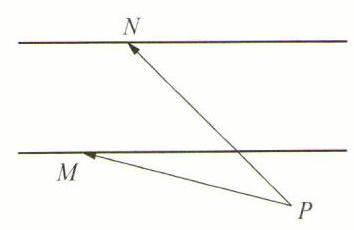
\includegraphics[width=0.3\textwidth]{bodyxb/src/bo_d1ig044601uc738hj6v0_52_1129_124_354_230_0.jpg}
\end{center}

第 6 题图

A. 15 B. 12

C. 10 D. 9

7. 已知点 $A\left( {-2,0}\right)$ ,设 $B\text{ 、 }C$ 是圆 $O : {x}^{2} + {y}^{2} = 1$ 上的两个不同的动点,且向量 $\vv{OB} = t\vv{OA} +$  $\left( {1 - t}\right) \vv{OC}$ (其中 $t$ 为实数),则 $\vv{AB} \cdot  \vv{AC} =$ \blkda{}.

\subsection*{27 “奔驰”定理}

\subsubsection*{知识点睛}

1. “奔驰”定理: $O$ 是 $\bigtriangleup {ABC}$ 内的一点,且 $x \cdot  \vv{OA} + y \cdot  \vv{OB} + z \cdot  \vv{OC} = \vv{0}$ ,则 ${S}_{\bigtriangleup {BOC}} : {S}_{\bigtriangleup {COA}} :$  ${S}_{\bigtriangleup {AOB}} = x : y : z.$

由于这个定理对应的图象和奔驰牌汽车的标志 (如图 1) 很相似, 我们把它称为 “奔驰” 定理.

2. “奔驰”定理的证明方法很多,这里提供一个参考版本.

如图 2,已知 $O$ 是 $\bigtriangleup  {ABC}$ 内的一点, $\bigtriangleup  {BOC}$ 、 $\bigtriangleup  {COA}$ 、 $\bigtriangleup  {AOB}$ 的面积分别为 ${S}_{A}$ 、 ${S}_{B}$ 、 ${S}_{C}$ ,求证: ${S}_{A} \cdot  \vv{OA} + {S}_{B} \cdot  \vv{OB} + {S}_{C} \cdot  \vv{OC} = \vv{0}$ .

证明: 延长 ${AO}$ 与 ${BC}$ 边相交于点 $D$ ,则 $\dfrac{BD}{DC} = \dfrac{{S}_{\bigtriangleup {ABD}}}{{S}_{\bigtriangleup {ACD}}} = \dfrac{{S}_{\bigtriangleup {BOD}}}{{S}_{\bigtriangleup {COD}}} =$  $\dfrac{{S}_{\bigtriangleup {ABD}} - {S}_{\bigtriangleup {BOD}}}{{S}_{\bigtriangleup {ACD}} - {S}_{\bigtriangleup {COD}}} = \dfrac{{S}_{C}}{{S}_{B}},\vv{OD} = \dfrac{DC}{BC}\vv{OB} + \dfrac{BD}{BC}\vv{OC} = \dfrac{{S}_{B}}{{S}_{B} + {S}_{C}}\vv{OB} +$  $\dfrac{{S}_{C}}{{S}_{B} + {S}_{C}}\vv{OC}$ . 因为 $\dfrac{OD}{OA} = \dfrac{{S}_{BOD}}{{S}_{BOA}} = \dfrac{{S}_{COD}}{{S}_{COA}} = \dfrac{{S}_{BOD} + {S}_{COD}}{{S}_{BOA} + {S}_{COA}} = \dfrac{{S}_{A}}{{S}_{B} + {S}_{C}}$ ,所以 $\vv{OD} =  - \dfrac{{S}_{A}}{{S}_{B} + {S}_{C}}\vv{OA}$ ,所以 $- \dfrac{{S}_{A}}{{S}_{B} + {S}_{C}}\vv{OA} = \dfrac{{S}_{B}}{{S}_{B} + {S}_{C}}\vv{OB} +$  $\dfrac{{S}_{C}}{{S}_{B} + {S}_{C}}\vv{OC}$ ,所以 ${S}_{A} \cdot  \vv{OA} + {S}_{B} \cdot  \vv{OB} + {S}_{C} \cdot  \vv{OC} = \vv{0}$ .

\begin{center}
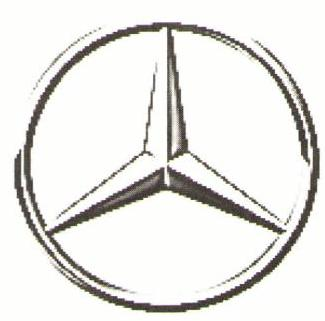
\includegraphics[width=0.2\textwidth]{bodyxb/src/bo_d1ig044601uc738hj6v0_53_1169_998_325_321_0.jpg}
\end{center}

图 1

\begin{center}
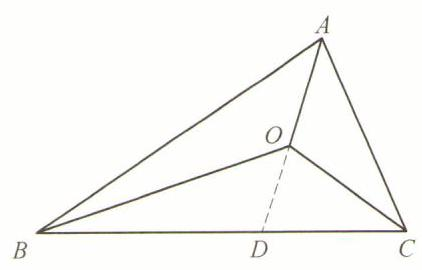
\includegraphics[width=0.3\textwidth]{bodyxb/src/bo_d1ig044601uc738hj6v0_53_1087_1404_422_270_0.jpg}
\end{center}

图 2

3. “奔驰” 定理的推论: 若 $x \cdot  \vv{OA} + y \cdot  \vv{OB} + z \cdot  \vv{OC} = \vv{0}$ ,则

① ${S}_{\bigtriangleup {BOC}} : {S}_{\bigtriangleup {COA}} : {S}_{\bigtriangleup {AOB}} = \left| x\right|  : \left| y\right|  : \left| z\right|$ ；

② $\dfrac{{S}_{\bigtriangleup {BOC}}}{{S}_{\bigtriangleup {ABC}}} = \left| \dfrac{x}{x + y + z}\right| ,\dfrac{{S}_{\bigtriangleup {AOC}}}{{S}_{\bigtriangleup {ABC}}} = \left| \dfrac{y}{x + y + z}\right| ,\dfrac{{S}_{\bigtriangleup {AOB}}}{{S}_{\bigtriangleup {ABC}}} =$  $\left| \dfrac{z}{x + y + z}\right|$ .

4. 对于三角形面积比例问题, 常规的做法一般是通过向量线性运算转化出三角形之间的关系. 但如果向量关系符合 “奔驰” 定理的形式, 在选择填空题中可以迅速得出正确答案.

\subsubsection*{经典习题}

1. 已知点 $M$ 是 $\bigtriangleup {ABC}$ 所在平面内的一点,若满足 $6\vv{AM} - \vv{AB} - 2\vv{AC} = \vv{0}$ ,且 ${S}_{\bigtriangleup {ABC}} = \lambda {S}_{\bigtriangleup {ABM}}$ , 则实数 $\lambda$ 的值是\blkda{}.

2. 设点 $O$ 在 $\bigtriangleup {ABC}$ 的内部,且 $\vv{AB} = 4\vv{OB} + 5\vv{OC}$ ,则 $\bigtriangleup {OAB}$ 的面积与 $\bigtriangleup {OBC}$ 的面积之比是\blkda{}.

3. 已知点 $A\text{ 、 }B\text{ 、 }C\text{ 、 }P$ 在同一平面内, $\vv{PQ} = \dfrac{1}{3}\vv{PA},\vv{QR} =$  $\dfrac{1}{3}\vv{QB},\vv{RP} = \dfrac{1}{3}\vv{RC}$ ,则 ${S}_{\bigtriangleup {ABC}} : {S}_{\bigtriangleup {PBC}}$ 等于(   ).

\begin{center}
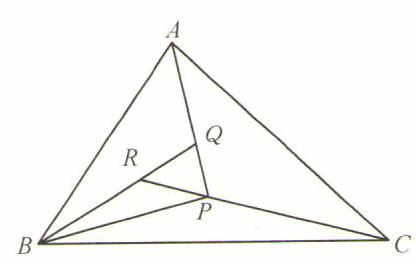
\includegraphics[width=0.3\textwidth]{bodyxb/src/bo_d1ig044601uc738hj6v0_54_1073_550_416_264_0.jpg}
\end{center}

第 3 题图

A. ${14} : 3$ B. ${19} : 4$

C. ${24} : 5$ D. ${29} : 6$

4. 点 $P$ 在 $\bigtriangleup {ABC}$ 所在平面上,且满足 $\vv{PA} + \vv{PB} + \vv{PC} = 2\vv{AB}$ , 则 $\dfrac{{S}_{\bigtriangleup {PAB}}}{{S}_{\bigtriangleup {ABC}}} =$ (   ).

A. $\dfrac{1}{2}$ B. $\dfrac{1}{3}$ C. $\dfrac{1}{4}$ D. $\dfrac{2}{3}$

5. 设 $P$ 为 $\bigtriangleup {ABC}$ 所在平面上一点,且满足 $3\vv{PA} + 4\vv{PC} = m\vv{AB}\left( {m > 0}\right)$ . 若 $\bigtriangleup {ABP}$ 的面积为 8,则 $\bigtriangleup  {ABC}$ 的面积为\blkda{}.

\subsection*{28 三角形的 “四心”}

\subsubsection*{知识点睛}

1. 三角形的重心 $G$ 是三角形三条中线的交点.

重心的性质 (图 1):

\begin{center}
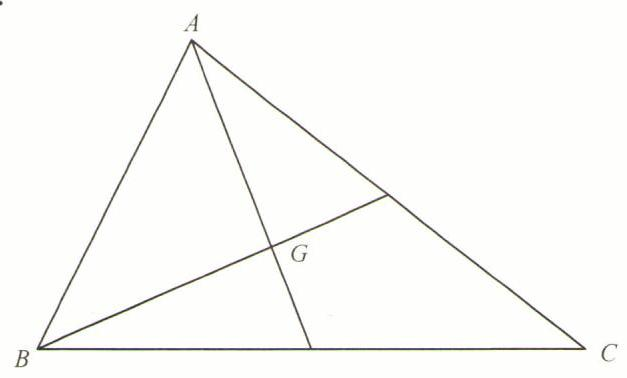
\includegraphics[width=0.5\textwidth]{bodyxb/src/bo_d1ig044601uc738hj6v0_55_879_560_627_378_0.jpg}
\end{center}

图 1

(1)重心到顶点的距离与重心到对边中点的距离之比为 $2 : 1$ ；

(2)重心和三角形三个顶点组成的三个三角形面积相等;

(3)在平面直角坐标系中,重心的坐标是三个顶点坐标的算术平均数,即 $\left( {\dfrac{{x}_{A} + {x}_{B} + {x}_{C}}{3},}\right.$  $\left. \dfrac{{y}_{A} + {y}_{B} + {y}_{C}}{3}\right)$ ;

(4)设 $G$ 是 $\bigtriangleup {ABC}$ 的重心,则 $\vv{GA} + \vv{GB} + \vv{GC} = \vv{0}$ ；

(5) $\vv{AG} = \dfrac{2}{3}\vv{AM} = \dfrac{1}{3}\left( {\vv{AB} + \vv{AC}}\right)$ .

2. 三角形的垂心 $O$ 是三角形三条高的交点.

\begin{center}
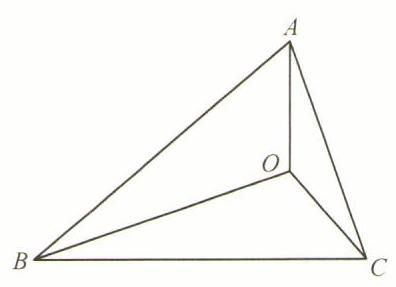
\includegraphics[width=0.3\textwidth]{bodyxb/src/bo_d1ig044601uc738hj6v0_55_1084_1299_396_287_0.jpg}
\end{center}

图 2

垂心的性质 (图 2):

(1) $\vv{OA} \cdot  \vv{OB} = \vv{OB} \cdot  \vv{OC} = \vv{OC} \cdot  \vv{OA}$ ；

(2) ${\left| \vv{OA}\right| }^{2} + {\left| \vv{BC}\right| }^{2} = {\left| \vv{OB}\right| }^{2} + {\left| \vv{CA}\right| }^{2} = {\left| \vv{OC}\right| }^{2} + {\left| \vv{AB}\right| }^{2}$ .

3. 三角形的内心 $P$ 是三角形三条角平分线的交点 (三角形内切圆的圆心).

内心的性质 (图 3):

\begin{center}
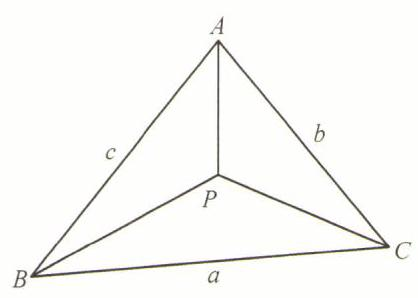
\includegraphics[width=0.3\textwidth]{bodyxb/src/bo_d1ig044601uc738hj6v0_55_1083_1646_418_298_0.jpg}
\end{center}

图 3

$\left| \vv{AB}\right| \vv{PC} + \left| \vv{BC}\right| \vv{PA} + \left| \vv{CA}\right| \vv{PB} = \vv{0}$ (或 $a\vv{PA} + b\vv{PB} +$  $c\vv{PC} = \vv{0}$ ),其中 $a\text{ 、 }b\text{ 、 }c$ 分别是 $\bigtriangleup {ABC}$ 的三边 ${BC}\text{ 、 }{AC}\text{ 、 }{AB}$ 的长.

4. 三角形的外心 $O$ 是三角形三边的垂直平分线的交点 (三角形外接圆的圆心).

外心的性质 (图 4):

\begin{center}
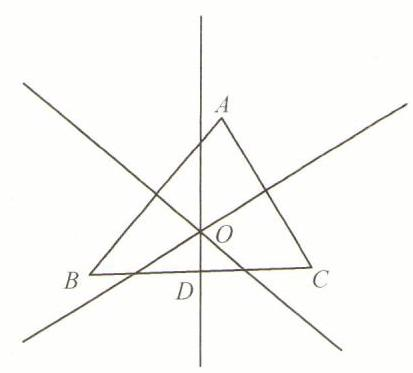
\includegraphics[width=0.3\textwidth]{bodyxb/src/bo_d1ig044601uc738hj6v0_56_1070_121_413_373_0.jpg}
\end{center}

图 4

三角形的外心 $O$ 到三角形三个顶点的距离相等, $\left| \vv{OA}\right|  =$  $\left| \vv{OB}\right|  = \left| \vv{OC}\right|  \Leftrightarrow  {\vv{OA}}^{2} = {\vv{OB}}^{2} = {\vv{OC}}^{2}.$

\subsubsection*{经典习题}

1. 若 $\bigtriangleup {ABC}$ 的内角 $A\text{ 、 }B\text{ 、 }C$ ,其中 $G$ 为 $\bigtriangleup {ABC}$ 的重心,且 $\vv{GA} \cdot  \vv{GB} = 0$ ,则 $\cos C$ 的最小值为\blkda{}.

2. $O$ 为 $\bigtriangleup {ABC}$ 平面内一定点,该平面内一动点 $P$ 满足 $M = \{ P\left| {\vv{OP} = \vv{OA} + \lambda (}\right| \vv{AB} \mid  \sin B$ . $\vv{AB} + \left| \vv{AC}\right| \sin C \cdot  \vv{AC}),\lambda  > 0\}$ ,则 $\bigtriangleup  {ABC}$ 的(   )一定属于集合 $M$ .

A. 重心 B. 垂心 C. 外心 D. 内心

3. 已知 $A,B,C$ 是平面上不共线的三点, $O$ 为坐标原点,动点 $P$ 满足 $\vv{OP} = \dfrac{1}{3}\lbrack \left( {1 - \lambda }\right) \vv{OA} +$  $\left( {1 - \lambda }\right) \vv{OB} + \left( {1 + {2\lambda }}\right) \vv{OC}\rbrack ,\lambda  \in  \mathbf{R}$ ,则点 $P$ 的轨迹一定经过 (   ).

A. $\bigtriangleup {ABC}$ 的内心 B. $\bigtriangleup {ABC}$ 的垂心

C. $\bigtriangleup {ABC}$ 的重心 D. $\bigtriangleup {ABC}$ 的中心

4. 已知点 $O$ 是非等边 $\bigtriangleup {ABC}$ 的外心, $P$ 是平面 ${ABC}$ 内的一点且 $\vv{OA} + \vv{OB} + \vv{OC} = \vv{OP}$ ,则 $P$ 是 $\bigtriangleup  {ABC}$ 的(   ).

A. 垂心 B. 重心 C. 内心 D. 外心

5. 已知 $O$ 是 $\bigtriangleup {ABC}$ 所在平面内一点,且满足 $\vv{BA} \cdot  \vv{OA} + {\left| \vv{BC}\right| }^{2} = \vv{AB} \cdot  \vv{OB} + {\left| \vv{AC}\right| }^{2}$ ,则点 $O$ (   ).

A. 在 ${AB}$ 边的高所在的直线上

B. 在 $\angle C$ 平分线所在的直线上

C. 在 ${AB}$ 边的中线所在的直线上

D. 是 $\bigtriangleup {ABC}$ 的外心

6. 若点 $O$ 在 $\bigtriangleup {ABC}$ 所在的平面内,满足 $\vv{OA} \cdot  \left( {\dfrac{\vv{AC}}{\left| \vv{AC}\right| } - \dfrac{\vv{AB}}{\left| \vv{AB}\right| }}\right)  = \vv{OB} \cdot  \left( {\dfrac{\vv{BC}}{\left| \vv{BC}\right| } - \dfrac{\vv{BA}}{\left| \vv{BA}\right| }}\right)  =$  $\vv{OC} \cdot  \left( {\dfrac{\vv{CA}}{\left| \vv{CA}\right| } - \dfrac{\vv{CB}}{\left| \vv{CB}\right| }}\right)  = 0$ ,则 $O$ 是 $\bigtriangleup  {ABC}$ 的(   ).

A. 垂心 B. 重心 C. 内心 D. 外心

7. 平面内 $\bigtriangleup {ABC}$ 及一点 $O$ 满足 $\dfrac{\vv{AO} \cdot  \vv{AB}}{\left| \vv{AB}\right| } = \dfrac{\vv{AO} \cdot  \vv{AC}}{\left| \vv{AC}\right| },\dfrac{\vv{CO} \cdot  \vv{CA}}{\left| \vv{CA}\right| } = \dfrac{\vv{CO} \cdot  \vv{CB}}{\left| \vv{CB}\right| }$ ,则点 $O$ 是 $\bigtriangleup {ABC}$ 的(   ).

A. 重心 B. 垂心 C. 内心 D. 外心

8. 已知点 $O$ 为 $\bigtriangleup {ABC}$ 所在平面内的一点,满足 $\vv{PO} = \dfrac{a\vv{PA} + b\vv{PB} + c\vv{PC}}{a + b + c}$ (其中 $P$ 是 $\bigtriangleup {ABC}$ 所在平面内任意的一点),则点 $O$ 为 $\bigtriangleup  {ABC}$ 的(   ).

A. 外心 B. 内心 C. 垂心 D. 重心

9. 设 $P$ 是 $\bigtriangleup {ABC}$ 所在平面内的一点,若 $\vv{AB} \cdot  \left( {\vv{CB} + \vv{CA}}\right)  = 2\vv{AB} \cdot  \vv{CP}$ 且 $\vv{A{B}^{2}} = \vv{A{C}^{2}} - 2\vv{BC}$ . $\vv{AP}$ ,则点 $P$ 是 $\bigtriangleup  {ABC}$ 的(   ).

A. 外心 B. 内心 C. 重心 D. 垂心

10. 设 $P$ 是 $\bigtriangleup {ABC}$ 所在平面内的一点,若 $\vv{AB} \cdot  \left( {\vv{CB} + \vv{CA}}\right)  = 2\vv{AB} \cdot  \vv{CP}$ ,且 $\left| \vv{AP}\right|  = \left| \vv{CP}\right|$ ,则点 $P$ 是 $\bigtriangleup  {ABC}$ 的(   ).

A. 外心 B. 内心 C. 重心 D. 垂心

\subsubsection*{知识点睛}

如图,平面内一组基底 $\vv{OB}$ 、 $\vv{OC}$ 及任一向量 $\vv{OA}$ ,有 $\vv{OA} = x\vv{OB} + y\vv{OC}\left( {x,y \in  \mathbf{R}}\right)$ ,若点 $A$ 在直线 ${BC}$ 或在平行于 ${BC}$ 的直线 $l$ 上,则 $x + y = k$ (定值),反之也成立,我们把直线 ${BC}$ 以及与 ${BC}$ 平行的直线叫做等和线.

(1)当等和线恰为直线 ${BC}$ 时, $k = 1$ ；

\begin{center}
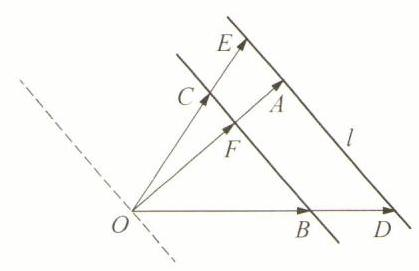
\includegraphics[width=0.3\textwidth]{bodyxb/src/bo_d1ig044601uc738hj6v0_58_1073_723_419_271_0.jpg}
\end{center}

(2)当等和线在点 $O$ 和直线 ${BC}$ 之间时, $k \in  \left( {0,1}\right)$ ；

(3)当直线 ${BC}$ 在点 $O$ 和等和线之间时, $k \in  \left( {1, + \infty }\right)$ ；

(4)当等和线过点 $O$ 时, $k = 0$ ；

(5)若两等和线关于点 $O$ 对称,则定值 $k$ 互为相反数；

(6)定值 $\left| k\right|$ 的变化与等和线到点 $O$ 的距离成正比.

\subsubsection*{经典习题}

1. 已知 $\bigtriangleup {ABC}$ 的外接圆圆心为 $O,\angle A = {120}^{ \circ  }$ ,若 $\vv{AO} = x\vv{AB} + y\vv{AC}\left( {x,y \in  \mathbf{R}}\right)$ ,则 $x + y$ 的最小值为 (   ).

A. $\dfrac{1}{2}$ B. $\dfrac{2}{3}$ C. $\dfrac{3}{2}$ D. 2

2. 已知 $\bigtriangleup {ABC}$ 的内角 $A\text{ 、 }B\text{ 、 }C$ 的对边分别为 $a\text{ 、 }b\text{ 、 }c$ ,且 $\cos A = \dfrac{7}{8},I$ 为 $\bigtriangleup  {ABC}$ 内部的一点,且 $a\vv{IA} + b\vv{IB} + c\vv{IC} = \vv{0}$ ,若 $\vv{AI} = x\vv{AB} + y\vv{AC}$ ,则 $x + y$ 的最大值为 (   ).

A. $\dfrac{5}{4}$ B. $\dfrac{1}{2}$ C. $\dfrac{5}{6}$ D. $\dfrac{4}{5}$

3. 已知 $O$ 为 $\bigtriangleup {ABC}$ 的外心, $\angle {ABC} = \dfrac{\pi }{3},\vv{BO} = \lambda \vv{BA} + \mu \vv{BC}$ ,则 $\lambda  + \mu$ 的最大值为\blkda{}.

4. 已知正六边形 ${ABCDEF}$ (顶点的字母依次按逆时针顺序确定) 的边长为 1 , 点 $P$ 是 $\bigtriangleup {CDE}$ 内 (含边界) 的动点,设 $\vv{AP} = x \cdot  \vv{AB} + y \cdot  \vv{AF}\left( {x,y \in  \mathbf{R}}\right)$ ,则 $x + y$ 的取值范围是\blkda{}.

5. 如图所示,将一圆的八个等分点分成相间的两组,连接每组的四个点得到两个正方形,去掉两个正方形内部的八条线段后可以形成一正八角星,设正八角星的中心为 $O$ ,并且 $\vv{OA} =$

$\vv{{e}_{1}},\vv{OB} = \vv{{e}_{2}}$ ,若将点 $O$ 到正八角星 16 个顶点的向量都写成 $\lambda \vv{{e}_{1}} + \mu \vv{{e}_{2}},\lambda ,\mu  \in  \mathbf{R}$ 的形式, 则 $\lambda  + \mu$ 的取值范围为 (   ).

A. $\left\lbrack  {-2\sqrt{2},2}\right\rbrack$ B. $\left\lbrack  {-2\sqrt{2},1 + \sqrt{2}}\right\rbrack$

C. $\left\lbrack  {-1 - \sqrt{2},1 + \sqrt{2}}\right\rbrack$ D. $\left\lbrack  {-1 - \sqrt{2},2}\right\rbrack$

\begin{center}
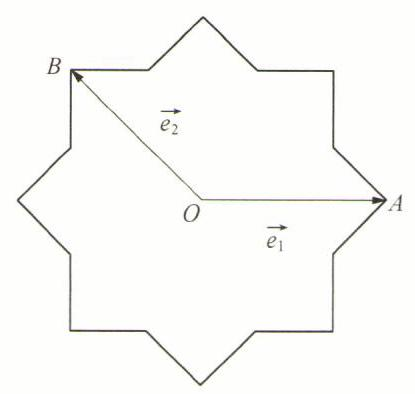
\includegraphics[width=0.3\textwidth]{bodyxb/src/bo_d1ig044601uc738hj6v0_59_314_408_415_394_0.jpg}
\end{center}

第 5 题图

\begin{center}
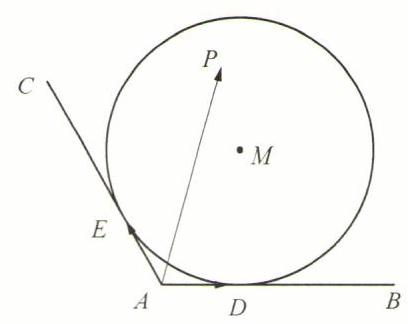
\includegraphics[width=0.3\textwidth]{bodyxb/src/bo_d1ig044601uc738hj6v0_59_914_473_408_324_0.jpg}
\end{center}

第 6 题图

6. 如图所示, $\angle {BAC} = \dfrac{2\pi }{3}$ ,圆 $M$ 与 ${AB}\text{ 、 }{AC}$ 分别相切于点 $D\text{ 、 }E,{AD} = 1$ ,点 $P$ 是圆 $M$ 及其内部任意一点,且 $\vv{AP} = x\vv{AD} + y\vv{AE}\left( {x,y \in  \mathbf{R}}\right)$ ,则 $x + y$ 的取值范围是 (   ).

A. $\left\lbrack  {1,4 + 2\sqrt{3}}\right\rbrack$ B. $\left\lbrack  {4 - 2\sqrt{3},4 + 2\sqrt{3}}\right\rbrack$

C. $\left\lbrack  {1,2 + \sqrt{3}}\right\rbrack$ D. $\left\lbrack  {2 - \sqrt{3},2 + \sqrt{3}}\right\rbrack$

\section*{立体几何}

立体几何是高中数学中非常浪漫的一个章节,需要同学们用自己的空间想象能力把三维的世界和二维的试题串起来. 那么具备一定的空间想象能力是解决立体几何问题的必要条件吗? 应该说是这样的. 同时我们也必须明确, 空间想象能力是可以培养出来的,它不是凭空的、任意的,而是基于四条公理,严谨推导得出的. 点线面可以组合出多种图形,但是万变不离其宗,最终研究的都是平行、垂直、夹角,以及 “长度”. 在高考数学中, 立体几何虽然占比不小, 却是比较温柔的考点, 总结出常见模型的规律之后, 很多答案都可以按部就班得到.

\subsection*{30 位置关系}

\subsubsection*{知识点睛}

点线面的位置关系,每一个都不是独立存在的,它们常常互相依存,可能需要从面面关系推出线线关系,再由线线关系推出线面关系等. 我们在解决问题的时候,要结合图形整体分析, 同时提醒大家,有些小技巧是很好用的,比如:直线与直线的位置关系可以一一考虑平行、相交和异面,再做出选择；线面关系,多关注两个相交平面的交线有且仅有一条,交线往往起到“交通枢纽”的作用；命题真假的判断,多放在我们熟悉的模型,比如正方体、长方体、四面体中进行对比；异面直线的成角问题,我们一般都会通过作平行线,转化成共面相交直线的夹角问题等.

\subsubsection*{经典习题}

\begin{center}
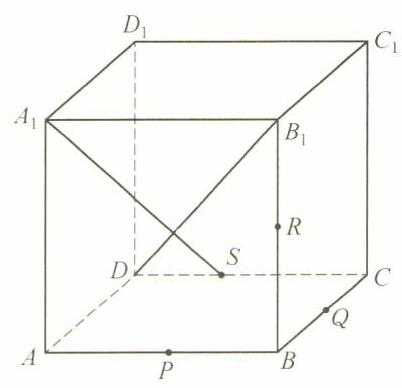
\includegraphics[width=0.3\textwidth]{bodyxb/src/bo_d1ig044601uc738hj6v0_61_1094_997_402_388_0.jpg}
\end{center}

第 1 题图

1. 如图,正方体 ${ABCD} - {A}_{1}{B}_{1}{C}_{1}{D}_{1}$ 中, $P\text{ 、 }Q\text{ 、 }R\text{ 、 }S$ 分别为棱 ${AB}\text{ 、 }{BC}\text{ 、 }B{B}_{1}\text{ 、 }{CD}$ 的中点,连接 ${A}_{1}S\text{ 、 }{B}_{1}D$ ,对空间任意两点 $M\text{ 、 }N$ ,若线段 ${MN}$ 与线段 ${A}_{1}S\text{ 、 }{B}_{1}D$ 都不相交,则称 $M\text{ 、 }N$ 两点可视,下列选项中与点 ${D}_{1}$ 可视的为 (   ).

A. 点 $P$ B. 点 $Q$

C. 点 $R$ D. 点 $B$

2. 已知 $\alpha \text{ 、 }\beta$ 是两个相交平面,空间两条直线 ${l}_{1}\text{ 、 }{l}_{2}$ 在 $\alpha$ 上的射影是直线 ${s}_{1}\text{ 、 }{s}_{2},{l}_{1}\text{ 、 }{l}_{2}$ 在 $\beta$ 上的射影是直线 ${t}_{1}\text{ 、 }{t}_{2}$ . 用 ${s}_{1}$ 与 ${s}_{2}$ 、 ${t}_{1}$ 与 ${t}_{2}$ 的位置关系,写出一个总能确定 ${l}_{1}$ 与 ${l}_{2}$ 是异面直线的充分条件:\blkda{}.

3. 在正方体 ${ABCD} - {A}_{1}{B}_{1}{C}_{1}{D}_{1}$ 中, $E\text{ 、 }F$ 分别为棱 $A{A}_{1}\text{ 、 }C{C}_{1}$ 的中点,则在空间中与 ${A}_{1}{D}_{1}$ 、 ${EF}\text{ 、 }{CD}$ 三条直线都相交的直线(   ).

A. 不存在 B. 有且只有两条

C. 有且只有三条 D. 有无数条

\begin{center}
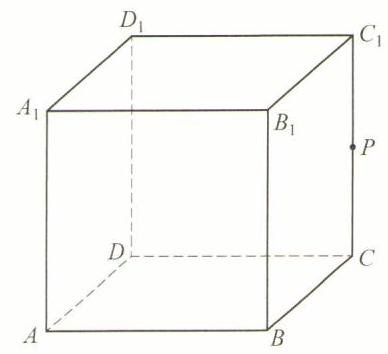
\includegraphics[width=0.3\textwidth]{bodyxb/src/bo_d1ig044601uc738hj6v0_61_1109_1747_388_354_0.jpg}
\end{center}

第 4 题图

4. 如图,已知正方体 ${ABCD} - {A}_{1}{B}_{1}{C}_{1}{D}_{1}$ ,点 $P$ 是棱 $C{C}_{1}$ 的中点,设直线 ${AB}$ 为 $a$ ,直线 ${A}_{1}{D}_{1}$ 为 $b$ . 对于下列两个命题:

① 过点 $P$ 有且只有一条直线与 $a$ 、 $b$ 都相交；

② 过点 $P$ 有且只有两条直线与 $a$ 、 $b$ 都成 ${75}^{ \circ  }$ 角.

以下判断中正确的是(   ).

A. ①为真命题,②为真命题

B. ①为真命题,②为假命题

C. ①为假命题,②为真命题

D. ①为假命题,②为假命题

5. 异面直线 $a\text{ 、 }b$ 成 ${80}^{ \circ  }$ 角,点 $P$ 是直线 $a\text{ 、 }b$ 外的一个定点,若过点 $P$ 有且仅有 2 条直线与 $a$ 、 $b$ 所成的角相等且等于 $\theta$ ,则 $\theta$ 的取值范围是\blkda{}.

6. 如图 1,在正方形 ${ABCD}$ 中,点 $M$ 是边 ${CD}$ 的中点,如图 2,将 $\bigtriangleup {ADM}$ 沿 ${AM}$ 翻折到 $\bigtriangleup {PAM}$ ,连接 ${PB}\text{ 、 }{PC}$ ,在 $\bigtriangleup {ADM}$ 翻折到 $\bigtriangleup {PAM}$ 的过程中,有下列三个说法:

\begin{center}
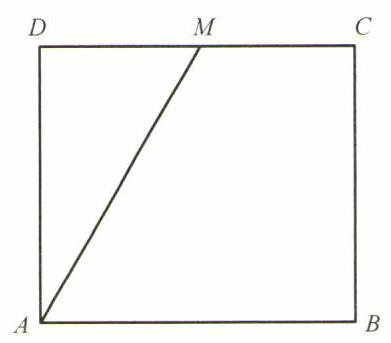
\includegraphics[width=0.3\textwidth]{bodyxb/src/bo_d1ig044601uc738hj6v0_62_387_608_391_343_0.jpg}
\end{center}

第 6 题图 1

\begin{center}
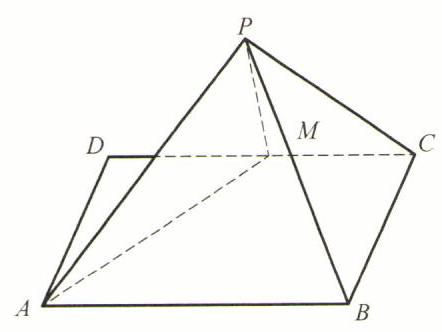
\includegraphics[width=0.3\textwidth]{bodyxb/src/bo_d1ig044601uc738hj6v0_62_866_616_442_332_0.jpg}
\end{center}

第 6 题图 2

① 点 $P$ 的轨迹为圆弧；

② 存在某一翻折位置,使得 ${AM} \bot  {PB}$ ；

③ 棱 ${PB}$ 的中点为 $E$ ,则 ${CE}$ 的长为定值.

其中,正确说法的序号有\blkda{}.

\subsection*{31 截面问题}

\subsubsection*{知识点睛}

我们先给出以下定义:用一个平面去截几何体,此平面与几何体的交集,叫做这个几何体的截面. 此平面与几何体表面的交集(交线)叫做截线. 此平面与几何体的棱的交集(交点)叫做截点.

一般来说,我们做截面的方法主要是交线法,即先确定截点,尤其是位于多面体同一表面的两个截点, 连起来就是这个平面的截线, 截线延长之后和其他棱的交点, 则是位于另一个表面的截点. 有两条截线平行的情况下, 也可以借助平行线快速找到截面. 要注意, 截面是一个平面闭合图形,并且每条边都在几何体的表面上.

\begin{center}
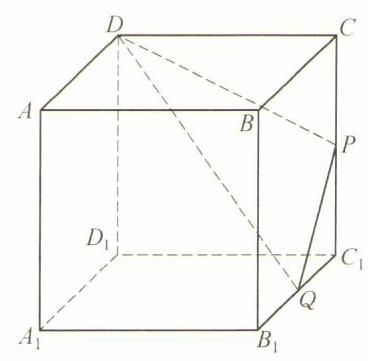
\includegraphics[width=0.3\textwidth]{bodyxb/src/bo_d1ig044601uc738hj6v0_63_1133_905_368_361_0.jpg}
\end{center}

第 1 题图

\subsubsection*{经典习题}

1. 如图,在棱长为 2 的正方体 ${ABCD} - {A}_{1}{B}_{1}{C}_{1}{D}_{1}$ 中, $P\text{ 、 }Q$ 分别为 $C{C}_{1}\text{ 、 }{B}_{1}{C}_{1}$ 的中点,则过 $D\text{ 、 }P\text{ 、 }Q$ 三点的平面截正方体 ${ABCD} - {A}_{1}{B}_{1}{C}_{1}{D}_{1}$ 所得截面的面积为\blkda{}.

2. 如图,棱长为 1 的正方体 ${ABCD} - {A}_{1}{B}_{1}{C}_{1}{D}_{1}$ 中, $P\text{ 、 }Q$ 分别在棱 ${BC}\text{ 、 }C{C}_{1}$ 上, ${CP} = x,{CQ} = y,x \in  \left\lbrack  {0,1}\right\rbrack  ,y \in  \left\lbrack  {0,1}\right\rbrack$ 且 ${x}^{2} + {y}^{2} \neq  0$ ,过 $A\text{ 、 }P\text{ 、 }Q$ 三点的平面截正方体 ${ABCD} -$  ${A}_{1}{B}_{1}{C}_{1}{D}_{1}$ 得到截面多边形,有下列四个说法:

\begin{center}
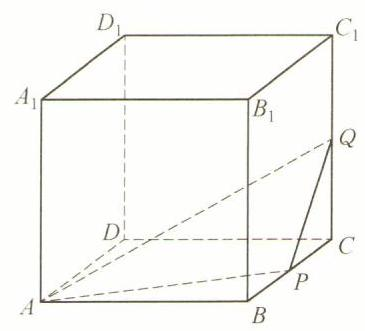
\includegraphics[width=0.3\textwidth]{bodyxb/src/bo_d1ig044601uc738hj6v0_63_1138_1319_365_331_0.jpg}
\end{center}

第 2 题图

① $x = y$ 时,截面一定为等腰梯形；

② $x = 1$ 时,截面一定为矩形且面积最大值为 $\sqrt{2}$ ；

③ 存在 $x,y$ 使截面为六边形；

④ 存在 $x,y$ 使 $B{D}_{1}$ 与截面平行.

其中, 正确说法的序号有\blkda{}.

3. 如图,棱长为 4 的正方体 ${ABCD} - {A}_{1}{B}_{1}{C}_{1}{D}_{1}$ 中,点 $E$ 、 $F$ 分别为 $D{D}_{1}\text{ 、 }{BC}$ 的中点,有下列四个结论:

\begin{center}
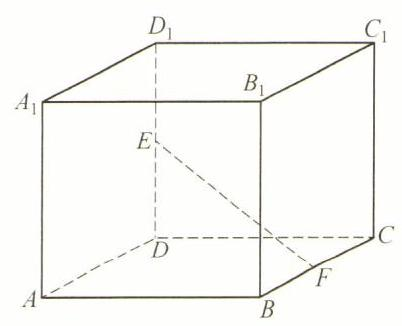
\includegraphics[width=0.3\textwidth]{bodyxb/src/bo_d1ig044601uc738hj6v0_63_1101_1753_402_326_0.jpg}
\end{center}

第 3 题图

① ${EF}\bot {A}_{1}D$ ；

② 直线 ${AE}$ 与平面 ${B}_{1}{CD}$ 所成角的正切值为 3 ；

③ ${EF}//$ 平面 ${A}_{1}B{D}_{1}$ ；

④ 平面 ${AEF}$ 截正方体 ${ABCD} - {A}_{1}{B}_{1}{C}_{1}{D}_{1}$ 的截面周长为

$4\sqrt{5} + 2\sqrt{6}$ .

其中,正确结论的序号有\blkda{}.

4. 如图,在棱长为 1 的正方体 ${ABCD} - {A}_{1}{B}_{1}{C}_{1}{D}_{1}$ 中, $M$ 为底面 ${ABCD}$ 的中心, $\vv{{D}_{1}Q} =$  $\lambda \vv{{D}_{1}{A}_{1}},\lambda  \in  \left( {0,1}\right) ,N$ 为线段 ${AQ}$ 的中点,有下列四个命题:

① ${CN}$ 与 ${QM}$ 共面;

\begin{center}
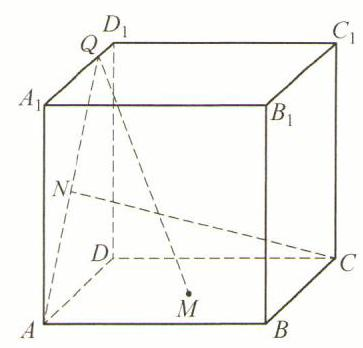
\includegraphics[width=0.3\textwidth]{bodyxb/src/bo_d1ig044601uc738hj6v0_64_1150_402_363_348_0.jpg}
\end{center}

第 4 题图

② 三棱锥 $A - {DMN}$ 的体积跟 $\lambda$ 的取值无关；

③ 当 $\lambda  = \dfrac{1}{3}$ 时,过 $A,Q,M$ 三点的平面截正方体所得截面的周长为 $\dfrac{4\sqrt{2} + 2\sqrt{13}}{3}$ ； ④ $\lambda  = \dfrac{1}{4}$ 时, ${AM} \bot  {QM}$ . 其中,正确命题的序号有\blkda{}.

5. 已知点 $E$ 、 $F$ 为正方体 ${ABCD} - {A}_{1}{B}_{1}{C}_{1}{D}_{1}$ 的棱 ${AB}\text{ 、 }{BC}$ 的中点, ${AB} = 4$ ,过 ${EF}$ 的平面 $\alpha$ 截正方体,有下列四个命题:

① 若 $\alpha$ 与底面 ${ABCD}$ 所成角的正切值为 $\sqrt{2}$ ,则截面为正六边形或正三角形；

② $\alpha$ 与底面 ${ABCD}$ 所成角为 ${45}^{ \circ  }$ ,则截面不可能为六边形；

③ 若截面为正三角形 ${EFG}$ 时,三棱锥 ${D}_{1} - {EFG}$ 的外接球的半径为 $\dfrac{9\sqrt{2}}{5}$ ；

④ 若截面为四边形,则截面与平面 ${B}_{1}{EF}$ 所成角的余弦值的最小值为 $\dfrac{7}{9}$ . 其中,正确命题的序号有\blkda{}.

\begin{center}
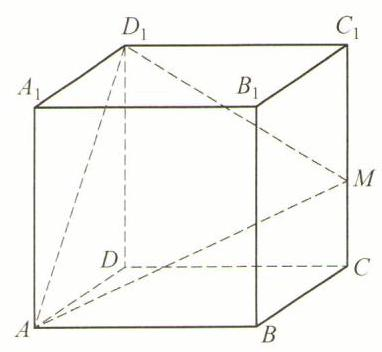
\includegraphics[width=0.3\textwidth]{bodyxb/src/bo_d1ig044601uc738hj6v0_64_1129_1317_382_352_0.jpg}
\end{center}

第 6 题图

6. 如图,已知正方体 ${ABCD} - {A}_{1}{B}_{1}{C}_{1}{D}_{1}$ 的棱长为 2,点 $M$ 为线段 $C{C}_{1}$ (含端点) 上的动点,由点 $A$ 、 ${D}_{1}$ 、 $M$ 确定的平面为 $\alpha$ , 有下列四个命题:

① 平面 $\alpha$ 截正方体的截面始终为四边形;

② 点 $M$ 运动过程中,三棱锥 ${A}_{1} - A{D}_{1}M$ 的体积为定值；

③ 平面 $\alpha$ 截正方体的截面面积的最大值为 $4\sqrt{2}$ ；

④ 三棱锥 ${A}_{1} - A{D}_{1}M$ 的外接球表面积的取值范围为 $\left\lbrack  {\dfrac{41}{4}\pi ,{12\pi }}\right\rbrack$ .

\begin{center}
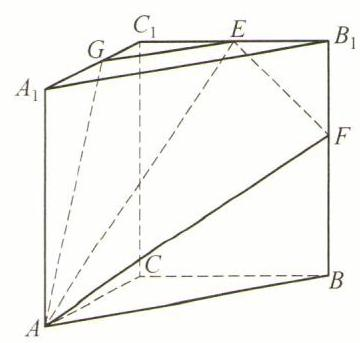
\includegraphics[width=0.3\textwidth]{bodyxb/src/bo_d1ig044601uc738hj6v0_64_1149_1747_360_343_0.jpg}
\end{center}

第 7 题图

其中,正确命题的序号有\blkda{}.

7. 如图,在直三棱柱 ${ABC} - {A}_{1}{B}_{1}{C}_{1}$ 中, $\angle {ACB} = {90}^{ \circ  },{AC} = {BC} =$  $C{C}_{1} = 2,E$ 为 ${B}_{1}{C}_{1}$ 的中点,过 ${AE}$ 的截面与棱 $B{B}_{1}\text{ 、 }{A}_{1}{C}_{1}$ 分别交于点 $F\text{ 、 }G$ ,则下列说法中正确的是 (   ).

A. 存在点 $F$ ,使得 ${A}_{1}F \bot  {AE}$

B. 线段 ${C}_{1}G$ 长度的取值范围是 $\left\lbrack  {0,1}\right\rbrack$

C. 当点 $F$ 与点 $B$ 重合时,四棱锥 $C - {AFEG}$ 的体积为 2

D. 设截面 ${AFEG}\text{ 、 }\bigtriangleup {AEG}\text{ 、 }\bigtriangleup {AEF}$ 的面积分别为 ${S}_{1}\text{ 、 }{S}_{2}\text{ 、 }{S}_{3}$ ,则 $\dfrac{{S}_{1}^{2}}{{S}_{2}{S}_{3}}$ 的最小值为 $2\sqrt{3}$

\subsection*{32 化折为直}

\subsubsection*{知识点睛}

化折为直,是解决空间几何体中两线段距离和的最值问题的一般方法,处理时将线段所在的平面展开,将立体问题转化为平面问题. 这里的平面首选是几何体表面,或者某些明显易确定的平面.

解决问题时,优先考虑将不同线段所在的平面通过翻折变为同一平面,再利用两点间线段最短求解.

如果涉及的线段都不在某个确定的平面内, 不能用平面展开来求解, 也不能用三角形两边之和大于第三边直接求解, 那么优先考虑对称求解.

如果两条线段前的系数不一样, 那么首先需要将线段前的系数变成相同的, 也就是通过不同线段的长度比例进行转化.

\subsubsection*{经典习题}

1. 如图,在直三棱柱 ${ABC} - {A}_{1}{B}_{1}{C}_{1}$ 中, $\angle {ACB} = {90}^{ \circ  },{AC} = 6$ , ${BC} = C{C}_{1} = \sqrt{2},P$ 是直线 $B{C}_{1}$ 上一动点,则 ${A}_{1}P + {PC}$ 的最小值是(   ).

\begin{center}
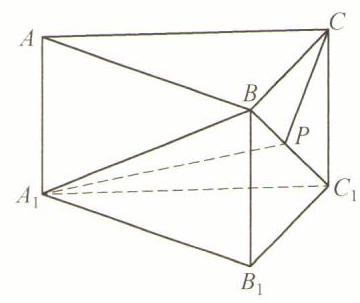
\includegraphics[width=0.3\textwidth]{bodyxb/src/bo_d1ig044601uc738hj6v0_66_1140_1211_360_303_0.jpg}
\end{center}

第 1 题图

A. $5\sqrt{2}$ B. $6 + \sqrt{2}$

C. ${10}\sqrt{2}$ D. ${12} + 2\sqrt{2}$

2. 如图,在棱长均为 $2\sqrt{3}$ 的正四面体 ${ABCD}$ 中, $M$ 为 ${AC}$ 的中点, $E$ 为 ${AB}$ 的中点, $P$ 是 ${DM}$ 上的动点, $Q$ 是平面 ${ECD}$ 上的动点, 则 ${AP} + {PQ}$ 的最小值是 (   ).

\begin{center}
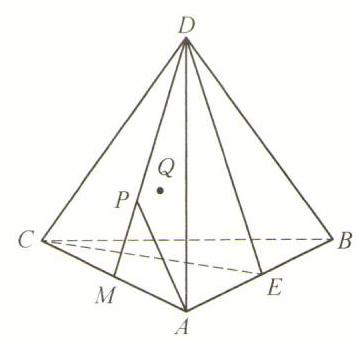
\includegraphics[width=0.3\textwidth]{bodyxb/src/bo_d1ig044601uc738hj6v0_66_1146_1594_360_343_0.jpg}
\end{center}

第 2 题图

A. $\dfrac{\sqrt{3} + \sqrt{11}}{2}$ B. $\sqrt{3} + \sqrt{2}$

C. $\dfrac{5}{4}\sqrt{3}$ D. $2\sqrt{3}$

3. 已知正方体 ${ABCD} - {A}^{\prime }{B}^{\prime }{C}^{\prime }{D}^{\prime }$ 的棱长为 $1,M\text{ 、 }N$ 分别为线段 $A{B}^{\prime }$ 、 ${AC}$ 上的动点,点 $T$ 在平面 ${BC}{C}^{\prime }{B}^{\prime }$ 内,则 $\left| {MT}\right|  +$

$\left| {NT}\right|$ 的最小值是 (   ).

A. $\sqrt{2}$ B. $\dfrac{2\sqrt{3}}{3}$

C. $\dfrac{\sqrt{6}}{2}$ D. 1

\begin{center}
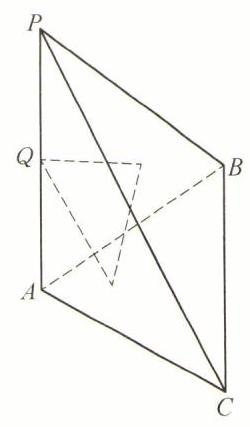
\includegraphics[width=0.2\textwidth]{bodyxb/src/bo_d1ig044601uc738hj6v0_67_1250_203_250_427_0.jpg}
\end{center}

第 4 题图

4. 如图,已知三棱锥 $P - {ABC}$ ,其中 ${PA} \bot$ 平面 ${ABC},{PA} = 3,\bigtriangleup {ABC}$ 是边长为 2 的正三角形. 已知 $Q$ 为棱 ${PA}$ (不含端点) 上的动点,若光线从点 $Q$ 出发,依次经过平面 ${PBC}$ 与平面 ${ABC}$ 反射后重新回到点 $Q$ ,则光线经过的路径长度的取值范围是(   ).

A.(0,6) B.(3,6)

C. $\left( {0,2\sqrt{3}}\right)$ D. $\left( {3,2\sqrt{3}}\right)$

5. 如图,在棱长为 1 的正方体 ${ABCD} - {A}_{1}{B}_{1}{C}_{1}{D}_{1}$ 中, $P$ 为线段 $A{B}_{1}$ 的中点, $M\text{ 、 }N$ 分别为线段 $A{C}_{1}$ 和棱 ${C}_{1}{D}_{1}$ 上任意一点,则 ${PM} + \dfrac{\sqrt{2}}{2}{MN}$ 的最小值为 (   ).

\begin{center}
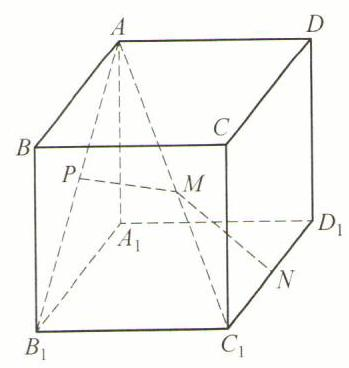
\includegraphics[width=0.2\textwidth]{bodyxb/src/bo_d1ig044601uc738hj6v0_67_1154_690_349_368_0.jpg}
\end{center}

第 5 题图

A. $\dfrac{\sqrt{2}}{4}$ B. $\dfrac{\sqrt{2}}{2}$

C. 1 D. $\sqrt{2}$

6. 如图,在棱长为 3 的正方体 ${ABCD} - {A}_{1}{B}_{1}{C}_{1}{D}_{1}$ 中, $P$ 为正方体表面 ${BC}{C}_{1}{B}_{1}$ 上的一个动点, $E\text{ 、 }F$ 分别为 $B{D}_{1}$ 的三等分点, 则 $\left| {PE}\right|  + \left| {PF}\right|$ 的最小值为 (   ).

\begin{center}
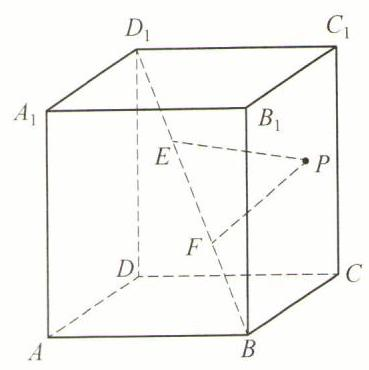
\includegraphics[width=0.3\textwidth]{bodyxb/src/bo_d1ig044601uc738hj6v0_67_1140_1119_369_370_0.jpg}
\end{center}

第 6 题图

A. $3\sqrt{3}$

B. $\dfrac{5\sqrt{2}}{2}$

C. $1 + \sqrt{6}$

D. $\sqrt{11}$

7. 如图,直三棱柱 ${ABC} - {A}_{1}{B}_{1}{C}_{1}$ 中, ${AB} = {AC} = 2,{A{A}_{1}} = 1$ , ${AB} \bot  {AC}$ ,点 $E$ 、 ${E}_{1}$ 分别是棱 ${BC}$ 、 ${B}_{1}{C}_{1}$ 的中点,点 $G$ 在棱 ${A}_{1}{B}_{1}$ 上,且 $G{B}_{1} = \sqrt{2}$ ,截面 $A{A}_{1}{E}_{1}E$ 内的动点 $P$ 满足 ${GB} \bot$  $P{E}_{1}$ ,则 ${PE} + P{B}_{1}$ 的最小值是 (   ).

\begin{center}
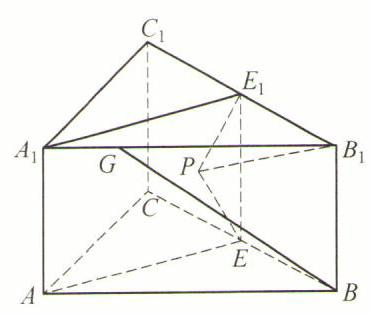
\includegraphics[width=0.3\textwidth]{bodyxb/src/bo_d1ig044601uc738hj6v0_67_1138_1568_371_314_0.jpg}
\end{center}

第 7 题图

A. $2 + \sqrt{2}$ B. $\sqrt{6}$

C. $\sqrt{5}$ D. 2

\subsection*{33 最大角和最小角问题}

\subsubsection*{知识点睛}

1. 最小角定理: 平面的斜线和它在平面内的射影所成的锐角 $\theta$ ,是这条斜线和平面内任一直线 ${AB}$ 所成角 $\angle {PAB}$ 中的最小值, 即线面角是最小的线线角. (如图 1, 由三余弦定理 $\cos \angle {PAB} = \cos \theta  \cdot  \cos \angle {OAB}$ 可得)

\begin{center}
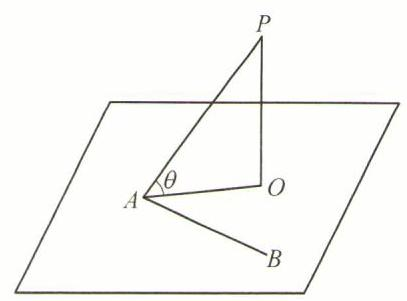
\includegraphics[width=0.3\textwidth]{bodyxb/src/bo_d1ig044601uc738hj6v0_68_1111_485_407_301_0.jpg}
\end{center}

图 1

2. 最大角定理:对于一个锐二面角,在其中一个半平面内的任一条直线与另一个半平面所成的线面角 $\theta$ 的最大值等于二面角的平面角 $\alpha$ ,即二面角是最大的线面角. (如图 2,由三正弦定理 $\sin \theta  = \sin \alpha  \cdot  \sin \angle {PAB}$ 可得)

\begin{center}
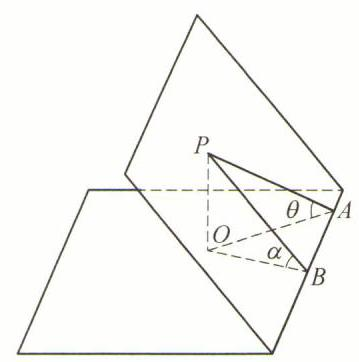
\includegraphics[width=0.3\textwidth]{bodyxb/src/bo_d1ig044601uc738hj6v0_68_1124_840_359_362_0.jpg}
\end{center}

图 2

3. 若二面角的一个半平面内有一条直线垂直于公共棱, 则此二面角的平面角等于该直线与另一个半平面所成的角, 即二面角与线面角可以相互转换.

\subsubsection*{经典习题}

1. 设三棱锥 $V - {ABC}$ 的底面是正三角形,侧棱长均相等, $P$ 是棱 ${VA}$ 上的点 (不含端点). 记直线 ${PB}$ 与直线 ${AC}$ 所成的角为 $\alpha$ ,直线 ${PB}$ 与平面 ${ABC}$ 所成的角为 $\beta$ ,二面角 $P - {AC} - B$ 的平面角为 $\gamma$ ,则 (   ).

A. $\beta  < \gamma ,\alpha  < \gamma$ B. $\beta  < \alpha ,\beta  < \gamma$

C. $\beta  < \alpha ,\gamma  < \alpha$ D. $\alpha  < \beta ,\gamma  < \beta$ 2. 如图,在矩形 ${ABCD}$ 中, ${AD} < {CD}$ ,现将 $\bigtriangleup {ACD}$ 沿 ${AC}$ 折起至 $\bigtriangleup {AC}{D}^{\prime }$ ,使二面角 $A - C{D}^{\prime } - B$ 的平面角为锐角, 设直线 $A{D}^{\prime }$ 与直线 ${BC}$ 所成的角为 $\alpha$ ,直线 $B{D}^{\prime }$ 与平面 ${ABC}$ 所成的角为 $\beta ,A{D}^{\prime }$ 与平面 ${BC}{D}^{\prime }$ 所成的角为 $\gamma$ ,则 (   ).

\begin{center}
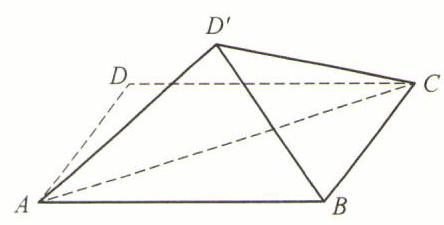
\includegraphics[width=0.3\textwidth]{bodyxb/src/bo_d1ig044601uc738hj6v0_68_1065_1716_444_225_0.jpg}
\end{center}

第 2 题图

A. $\alpha  > \beta  > \gamma$ B. $\alpha  > \gamma  > \beta$

C. $\beta  > \alpha  > \gamma$ D. $\gamma  > \alpha  > \beta$

3. 如图,在 $\bigtriangleup {ABC}$ 中, ${AB} = 1,{BC} = 2\sqrt{2},\angle B = \dfrac{\pi }{4}$ ,将 $\bigtriangleup {ABC}$ 绕边 ${AB}$ 翻转至 $\bigtriangleup {ABP}$ ,使平面 ${ABP} \bot$ 平面 ${ABC},D$ 是边 ${BC}$ 的中点,设 $Q$ 是线段 ${PA}$ 上的动点,当 ${PC}$ 与 ${DQ}$ 所成的角取得最小值时,线段 ${AQ}$ 的长度为\blkda{}.

\begin{center}
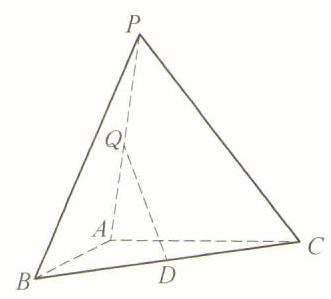
\includegraphics[width=0.2\textwidth]{bodyxb/src/bo_d1ig044601uc738hj6v0_69_1169_124_331_299_0.jpg}
\end{center}

第 3 题图

4. 如图,在三棱柱 ${ABC} - {A}_{1}{B}_{1}{C}_{1}$ 中, ${AB}\text{ 、 }{AC}\text{ 、 }A{A}_{1}$ 两两互相垂直, ${AB} = {AC} = A{A}_{1},M\text{ 、 }N$ 是线段 $B{B}_{1}\text{ 、 }C{C}_{1}$ 上的点,平面 ${AMN}$ 与平面 ${ABC}$ 所成(锐)二面角为 $\dfrac{\pi }{6}$ . 当 $\left| {{B}_{1}M}\right|$ 最小时, $\angle {AMB} =$ (   ).

A. $\dfrac{5\pi }{12}$ B. $\dfrac{\pi }{3}$ C. $\dfrac{\pi }{4}$ D. $\dfrac{\pi }{6}$

5. 在四面体 ${ABCD}$ 中, $\bigtriangleup {BCD}$ 为等边三角形, $\angle {ADB} = \dfrac{\pi }{2}$ ,二面角 $B - {AD} - C$ 的大小为 $\alpha$ , 则 $\alpha$ 的取值范围是 (   ).

A. $\left( {0,\dfrac{\pi }{6}}\right\rbrack$ B. $\left( {0,\dfrac{\pi }{4}}\right\rbrack$ C. $\left( {0,\dfrac{\pi }{3}}\right\rbrack$ D. $\left( {0,\dfrac{\pi }{2}}\right\rbrack$

\begin{center}
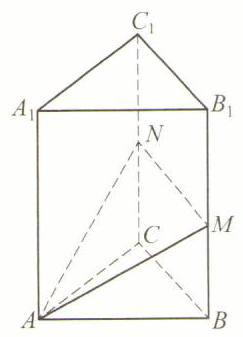
\includegraphics[width=0.2\textwidth]{bodyxb/src/bo_d1ig044601uc738hj6v0_69_172_1006_243_337_0.jpg}
\end{center}

第 4 题图

\begin{center}
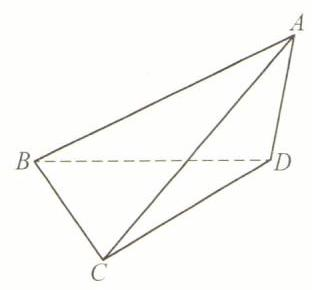
\includegraphics[width=0.2\textwidth]{bodyxb/src/bo_d1ig044601uc738hj6v0_69_456_1053_312_290_0.jpg}
\end{center}

第 5 题图

\begin{center}
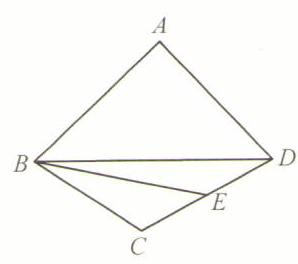
\includegraphics[width=0.2\textwidth]{bodyxb/src/bo_d1ig044601uc738hj6v0_69_813_1076_298_264_0.jpg}
\end{center}

第 6 题图 1

\begin{center}
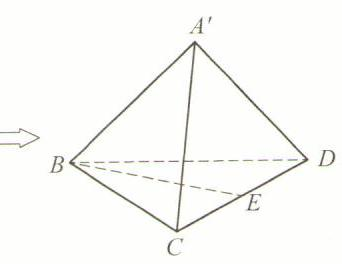
\includegraphics[width=0.2\textwidth]{bodyxb/src/bo_d1ig044601uc738hj6v0_69_1138_1072_342_264_0.jpg}
\end{center}

第 6 题图 2

6. 如图,在四边形 ${ABCD}$ 中, ${AB} = {BC} = {CD} = 2,{AD} = \sqrt{5}$ ,对角线 ${BD} = 3,E$ 是线段 ${CD}$ 上除端点外任一点,将 $\bigtriangleup {ABD}$ 沿 ${BD}$ 翻折成 $\bigtriangleup {A}^{\prime }{BD}$ ,使二面角 ${A}^{\prime } - {BD} - C$ 的大小为 ${120}^{ \circ  }$ , 设异面直线 ${A}^{\prime }D$ 和 ${BE}$ 所成的角为 $\alpha$ ,则 $\sin \alpha$ 的最小值是\blkda{}.

7. 如图,已知正四面体 $A - {BCD}$ , $\bigtriangleup {BCD}$ 在平面 $\alpha$ 内,点 $E$ 在线段 ${AC}$ 上, ${AE} = {2EC},l$ 是平面 $\alpha$ 的垂线. 在该四面体绕 ${CD}$ 旋转的过程中,直线 ${BE}$ 与 $l$ 所成的角为 $\theta$ ,则 $\sin \theta$ 的最小值是 (   ).

\begin{center}
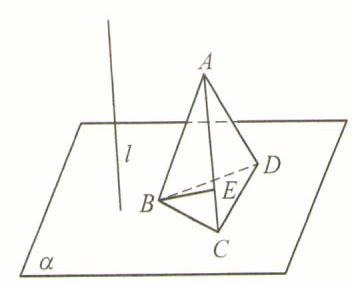
\includegraphics[width=0.3\textwidth]{bodyxb/src/bo_d1ig044601uc738hj6v0_69_1152_1625_354_284_0.jpg}
\end{center}

第 7 题图

A. $\dfrac{\sqrt{7}}{7}$ B. $\dfrac{\sqrt{3}}{6}$

C. $\dfrac{2\sqrt{21}}{21}$ D. $\dfrac{\sqrt{7}}{14}$

\subsection*{34 空间想象力}

\subsubsection*{知识点睛}

空间想象力的考核主要有两个大的方面:一个是能够把立体图形转化为平面图形,熟悉斜二测画法, 以及能够通过直线与平面的垂直, 快速找到点与线段在另一个平面上的射影, 将三维问题二维化;另一个就是能够通过文字描述和现实生活中的事例, 构造出符合要求的几何体立体模型,并且拆解成我们熟悉的常见几何体,比如棱柱、棱锥、圆柱、圆锥,还有球体,进而细分到点线面的位置关系,把问题放到平面图形中来解决.

\subsubsection*{经典习题}

1. 如图,正方体 ${ABCD} - {A}_{1}{B}_{1}{C}_{1}{D}_{1}$ 中,若 $E\text{ 、 }F$ 分别是 $A{A}_{1}\text{ 、 }{D}_{1}{C}_{1}$ 的中点, $G$ 是正方形 ${BC}{C}_{1}{B}_{1}$ 的中心,则空间四边形 ${AEFG}$ 在该正方体的面上的射影不可能是(   ).

\begin{center}
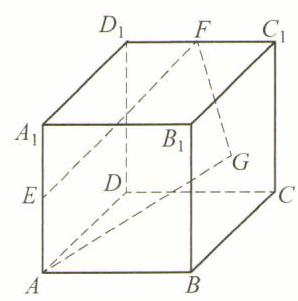
\includegraphics[width=0.2\textwidth]{bodyxb/src/bo_d1ig044601uc738hj6v0_70_1199_1038_298_301_0.jpg}
\end{center}

第 1 题图

\begin{center}
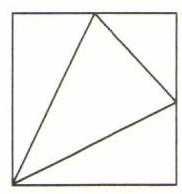
\includegraphics[width=0.2\textwidth]{bodyxb/src/bo_d1ig044601uc738hj6v0_70_250_1194_182_194_0.jpg}
\end{center}

A

\begin{center}
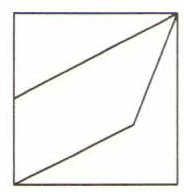
\includegraphics[width=0.2\textwidth]{bodyxb/src/bo_d1ig044601uc738hj6v0_70_483_1194_184_192_0.jpg}
\end{center}

B

\begin{center}
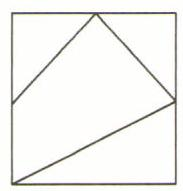
\includegraphics[width=0.2\textwidth]{bodyxb/src/bo_d1ig044601uc738hj6v0_70_719_1194_183_191_0.jpg}
\end{center}

C

\begin{center}
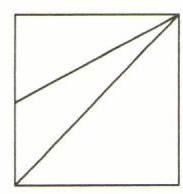
\includegraphics[width=0.2\textwidth]{bodyxb/src/bo_d1ig044601uc738hj6v0_70_950_1192_183_194_0.jpg}
\end{center}

D

2. 四面体 ${ABCD}$ 的所有棱长都为 1,棱 ${AB}//$ 平面 $\alpha$ ,则四面体上的所有点在平面 $\alpha$ 内的射影构成的图形面积的取值范围是\blkda{}.

3. 如图,直线 $l$ 垂直于平面 $\alpha$ ,垂足为 $O$ ,四面体 ${ABCD}$ 的棱长都为 $4,C$ 在平面 $\alpha$ 内, $B$ 是直线 $l$ 上的动点,则当 $O$ 到 ${AD}$ 距离最大时,四面体 ${ABCD}$ 在平面 $\alpha$ 上的射影面积为(   ).

\begin{center}
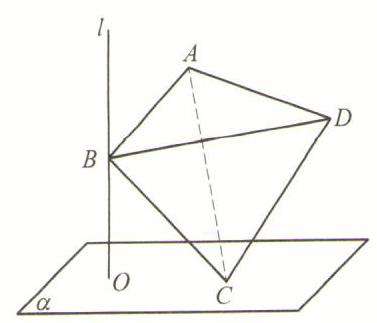
\includegraphics[width=0.3\textwidth]{bodyxb/src/bo_d1ig044601uc738hj6v0_70_1126_1562_377_323_0.jpg}
\end{center}

第 3 题图

A. $4 + 2\sqrt{2}$ B. $2 + 2\sqrt{2}$

C. $1 + \dfrac{\sqrt{2}}{2}$ D. 4

4. 将一个正方体切一刀, 可能得到以下几何体的种类数为 (   ).

①四面体；②四棱锥；③四棱柱；④五棱锥；⑤五棱柱；⑥六棱锥；⑦七面体.

A. 3 种 B. 4 种

C. 5 种 D. 以上均不正确

5. 如图,将正四面体每条棱三等分,截去顶角所在的小正四面体, 余下的多面体就成为一个半正多面体,亦称 “阿基米德体”,点 $A\text{ 、 }B\text{ 、 }M$ 是该多面体的三个顶点,点 $N$ 是该多面体表面上的动点,且总满足 ${MN} \bot  {AB}$ ,若 ${AB} =$ 4,则该多面体的表面积为\blkda{},点 $N$ 轨迹的长度为\blkda{}.

\begin{center}
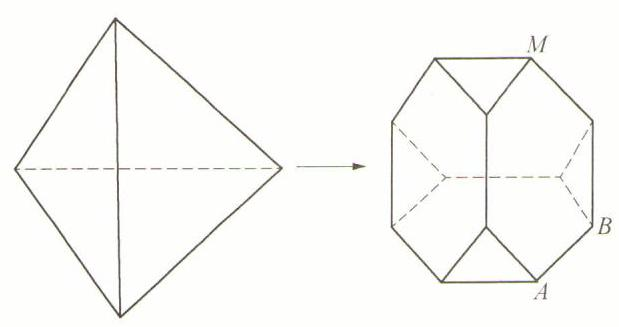
\includegraphics[width=0.5\textwidth]{bodyxb/src/bo_d1ig044601uc738hj6v0_71_873_244_619_327_0.jpg}
\end{center}

第 5 题图

6. 有四根长都为 2 的直铁条,若再选两根长都为 $a$ 的直铁条,使这六根铁条端点处相连能够焊接成一个四面体的铁框架,则 $a$ 的取值范围为\blkda{}.

7. 如图,“十字歇山”是由两个直三棱柱重叠后的景象,重叠后的底面为正方形,直三棱柱的底面是顶角为 ${120}^{ \circ  }$ ,腰为 3 的等腰三角形,则该几何体的体积为(   ).

\begin{center}
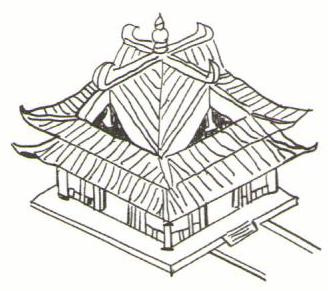
\includegraphics[width=0.2\textwidth]{bodyxb/src/bo_d1ig044601uc738hj6v0_71_389_906_328_291_0.jpg}
\end{center}

第 7 题图 1

\begin{center}
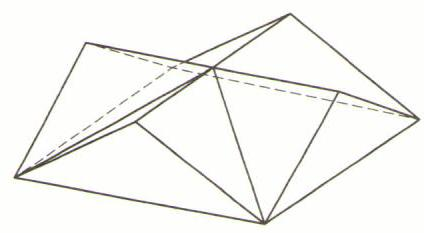
\includegraphics[width=0.3\textwidth]{bodyxb/src/bo_d1ig044601uc738hj6v0_71_878_960_424_233_0.jpg}
\end{center}

第 7 题图 2

A. 23 B. 24 C. 26 D. 27

8. 如图,一个“皇冠”状的空间图形由一个正方形和四个正三角形组成,并且正方形与每个正三角形所成的二面角的大小均为 $\theta$ ,如果把两个这样的 “皇冠” 倒扣在一起,可以围成一个十面体,则 $\cos \theta  =$ \blkda{}.

\begin{center}
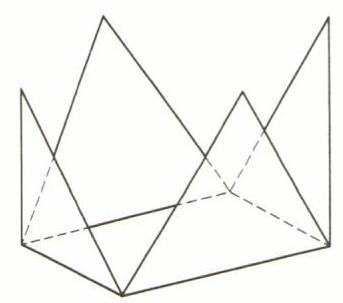
\includegraphics[width=0.2\textwidth]{bodyxb/src/bo_d1ig044601uc738hj6v0_71_429_1565_343_303_0.jpg}
\end{center}

第 8 题图 1

\begin{center}
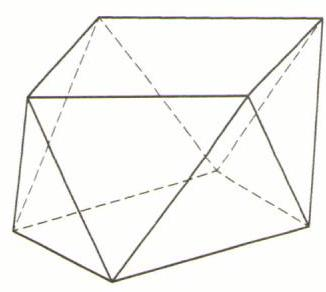
\includegraphics[width=0.2\textwidth]{bodyxb/src/bo_d1ig044601uc738hj6v0_71_927_1576_326_292_0.jpg}
\end{center}

第 8 题图 2

\subsection*{35 球}
\subsubsection*{知识点睛}

球体相关问题的压轴题, 主要会涉及多面体的外接球和内切球, 提醒大家注意以下知识点:

1. 外接球的定义:若一个多面体的各个顶点都在一个球的球面上,则称这个多面体是这个球的内接多面体, 这个球是这个多面体的外接球.

2. 外接球球心到多面体各顶点距离相等,它在底面上的投影是底面的外心,同时它在任意两顶点连线的中垂线上.

3. 内切球的定义:若一个多面体的各个面都与一个球的球面相切,则称这个多面体是这个球的外切多面体, 这个球是这个多面体的内切球.

4. 内切球球心到各表面距离相等.

5. 正多面体的内切球和外接球的球心重合. 正棱锥的内切球和外接球球心都在高线上,但不一定重合.

6. 确定球心后,构造三角形利用相似比和勾股定理是求半径的利器.

7. 体积分割法 (等体积法) 是求内切球半径的通用做法.

8. 两个几何体的交线问题, 先要确定交线的轨迹是什么, 再去求解.

\subsubsection*{经典习题}

1. 正三棱柱的顶点都在同一个球面上, 若球的半径为 4 , 则该三棱柱的侧面面积的最大值为 (   ).

A. ${48}\sqrt{3}$ B. ${64}\sqrt{3}$

C. $\dfrac{1728}{31}$ D. $\dfrac{576}{7}$

2. 已知直四棱柱 ${ABCD} - {A}_{1}{B}_{1}{C}_{1}{D}_{1}$ 的棱长均为 $2,\angle {BAD} = {60}^{ \circ  }$ . 以 ${D}_{1}$ 为球心, $\sqrt{5}$ 为半径的球面与侧面 ${B}_{1}{BC}{C}_{1}$ 的交线长为\blkda{}.

3. 已知同底面的两个正三棱锥 $P - {ABC}$ 和 $Q - {ABC}$ 均内接于球 $O$ ,且正三棱锥 $P - {ABC}$ 的侧面与底面所成角的大小为 $\dfrac{\pi }{4}$ ,则下列说法正确的是\blkda{}.

① ${PA}//$ 平面 ${QBC}$

② 设三棱锥 $Q - {ABC}$ 和 $P - {ABC}$ 的体积分别为 ${V}_{Q - {ABC}}$ 和 ${V}_{P - {ABC}}$ ,则 ${V}_{Q - {ABC}} = 4{V}_{P - {ABC}}$

③ 平面 ${ABC}$ 截球 $O$ 所得的截面面积是球 $O$ 表面积的 $\dfrac{4}{25}$

④ 二面角 $P - {AB} - Q$ 的正切值为 $- \dfrac{5}{3}$

4. 如图,在三棱锥 $S - {ABC}$ 中, ${SB}\bot {AB},{SB}\bot {BC},{AB}\bot$  ${BC},{SB} = {AB} = {BC} = 2,P,Q$ 分别为棱 ${AB},{BC}$ 的中点, $O$ 为三棱锥 $S - {ABC}$ 外接球的球心,则球 $O$ 的体积为\blkda{}；平面 ${SPQ}$ 截球 $O$ 所得截面的周长为\blkda{}.

\begin{center}
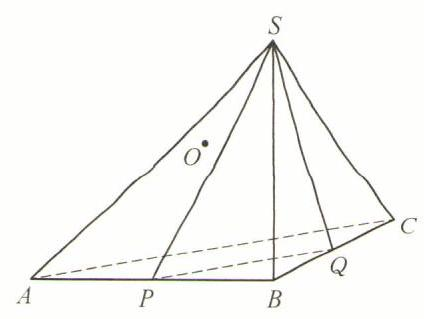
\includegraphics[width=0.3\textwidth]{bodyxb/src/bo_d1ig044601uc738hj6v0_73_1073_584_424_319_0.jpg}
\end{center}

第 4 题图

5. 已知一个正四面体的棱长为 2 , 则其外接球与以其一个顶点为球心, 1 为半径的球面所形成的交线的长度为\blkda{}.

6. 在正三棱锥 $P - {ABC}$ 中,侧棱 ${PA} = \sqrt{3}$ ,且侧棱 ${PA}\text{ 、 }{PB}\text{ 、 }{PC}$ 两两互相垂直,以 $A$ 为球心, 2 为半径的球面与正三棱锥的表面相交, 则交线的长度之和为\blkda{}.

7. 根据高中的解析几何知识, 我们知道平面与圆锥面相交时, 根据相交的角度不同,可以是三角形、圆、椭圆、抛物线、双曲线. 如图, ${AB}$ 是圆锥底面圆 $O$ 的直径,圆锥的母线 ${PA} = 2$ , ${AB} = 2\sqrt{2},E$ 是其母线 ${PB}$ 的中点. 若平面 $\alpha$ 过点 $E$ ,且 ${PB} \bot$ 平面 $\alpha$ ,则平面 $\alpha$ 与圆锥侧面的交线是以 $E$ 为顶点的抛物线的一部分,此时抛物线的焦点 $F$ 到底面圆心 $O$ 的距离为\blkda{}；截面 α 把圆锥分割成两部分,在两部分内部,

\begin{center}
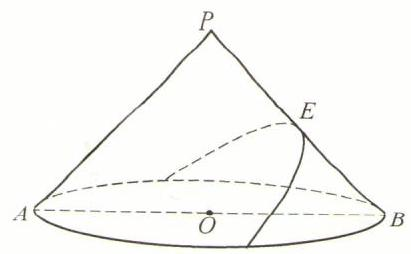
\includegraphics[width=0.3\textwidth]{bodyxb/src/bo_d1ig044601uc738hj6v0_73_1081_1165_411_254_0.jpg}
\end{center}

第 7 题图

在截面 $\alpha$ 的上方作一个半径最大的球 $M$ ,同时在截面 $\alpha$ 下方作一个半径最大的球 $N$ ,则球 $M$ 与球 $N$ 的半径的比值为\blkda{}.

\subsection*{36 最值问题}

\subsubsection*{知识点睛}

立体几何中的最值问题有三类:一是空间几何体中相关的点、线和面在运动, 求线段长度、 截面的面积和体积的最值; 二是空间几何体中相关点和线段在运动, 求有关角度和距离的最值；三是在空间几何体中,已知某些量的最值,确定点、线和面之间的位置关系.

一般可以从三方面着手:一是从问题的几何特征入手,充分利用其几何性质去解决；二是利用空间几何体的侧面展开图; 三是找出问题中的代数关系, 建立目标函数, 利用代数方法求目标函数的最值. 解题途径很多, 在函数建成后, 可用一次函数的端点法, 二次函数的配方法、 公式法, 函数有界法 (如三角函数等) 及导数法等.

\subsubsection*{经典习题}

1. 如图,在正方体 ${ABCD} - {A}_{1}{B}_{1}{C}_{1}{D}_{1}$ 中, ${AB} = 2,M,N$ 分别为 ${A}_{1}{D}_{1},{B}_{1}{C}_{1}$ 的中点, $E,F$ 分别为棱 ${AB},{CD}$ 上的动点,则三棱锥 $M - {NEF}$ 的体积 (   ).

A. 存在最大值,最大值为 $\dfrac{8}{3}$ B. 存在最小值,最小值为 $\dfrac{2}{3}$

C. 为定值 $\dfrac{4}{3}$ D. 不确定,与 $E,F$ 的位置有关

\begin{center}
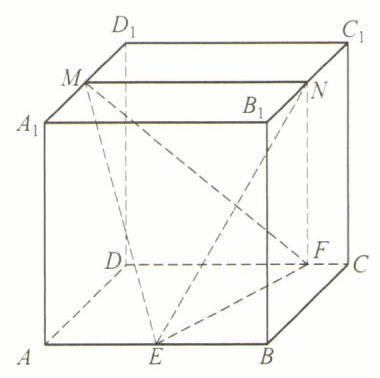
\includegraphics[width=0.3\textwidth]{bodyxb/src/bo_d1ig044601uc738hj6v0_74_352_1479_380_378_0.jpg}
\end{center}

第 1 题图

\begin{center}
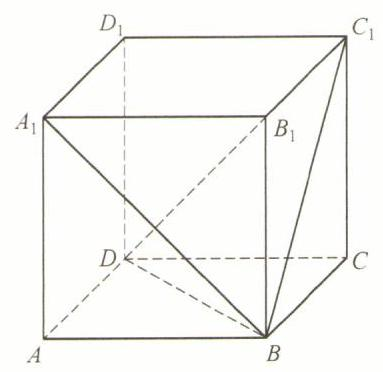
\includegraphics[width=0.3\textwidth]{bodyxb/src/bo_d1ig044601uc738hj6v0_74_918_1479_383_372_0.jpg}
\end{center}

第 2 题图

2. 如图,在棱长为 $2\sqrt{2}$ 的正方体 ${ABCD} - {A}_{1}{B}_{1}{C}_{1}{D}_{1}$ 中,若 $\bigtriangleup {AB}{A}_{1}$ 绕 ${A}_{1}B$ 旋转一周,则在旋转过程中,三棱锥 $A - {BD}{C}_{1}$ 的体积的取值范围为\blkda{}.

3. 在 $\bigtriangleup {ABC}$ 中, $\angle {BAC} = {90}^{ \circ  },{AB} = 6,{AC} = 8,D$ 是斜边上一点,以 ${AD}$ 为棱折成二面角 $C - {AD} - B$ ,其大小为 ${60}^{ \circ  }$ ,则折后线段 ${BC}$ 的最小值为\blkda{}.

\begin{center}
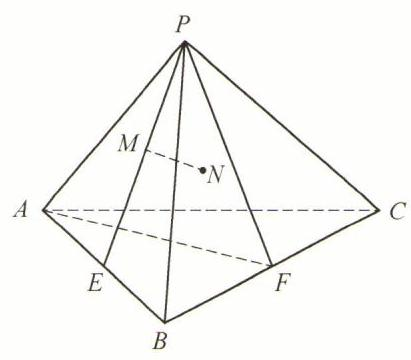
\includegraphics[width=0.3\textwidth]{bodyxb/src/bo_d1ig044601uc738hj6v0_75_1083_131_411_360_0.jpg}
\end{center}

第 4 题图

4. 在侧棱长为 $\sqrt{2}$ ,底面边长为 2 的正三棱锥 $P - {ABC}$ 中, $E$ , $F$ 分别为 ${AB},{BC}$ 的中点, $M,N$ 分别为 ${PE}$ 和平面 ${PAF}$ 上的动点,则 ${BM} + {MN}$ 的最小值为\blkda{}.

5. 长方体 ${ABCD} - {A}_{1}{B}_{1}{C}_{1}{D}_{1}$ 中, ${AB} = {BC} = 1,A{A}_{1} = 2$ ,平面 $A{B}_{1}C$ 与直线 ${D}_{1}{C}_{1}$ 的交点为 $M$ ,现将 $\bigtriangleup {MC}{B}_{1}$ 绕 $C{B}_{1}$ 旋转一周,在旋转过程中,动直线 ${CM}$ 与底面 ${A}_{1}{B}_{1}{C}_{1}{D}_{1}$ 内任一直线所成最小角记为 $\alpha$ ,则 $\sin \alpha$ 的最大值是\blkda{}.

6. 在 $\bigtriangleup {OAB}$ 中, ${OA} = {AB} = 4,\angle {OAB} = {120}^{ \circ  }$ ,若空间点 $P$ 满足 ${S}_{\bigtriangleup {PAB}} = \dfrac{1}{2}{S}_{\bigtriangleup {OAB}}$ ,则 ${OP}$ 的最小值为\blkda{}；直线 ${OP}$ 与平面 ${OAB}$ 所成角的正切的最大值是\blkda{}.

\section*{圆锥曲线}

圆锥曲线是高中解析几何的核心内容,解析几何的本质是用代数的方法研究几何问题的性质, 是数学的热点, 我们在尝试把几何图形数字化. 在学习过程中, 同学们要有探究精神,对椭圆、双曲线、抛物线、圆的性质都可以类比分析,总结规律. 高考试题中,解析几何在解答题中往往兼顾计算能力的考核,而在填选题目中,对圆锥曲线定义、性质、化归的考核更多一些.

\subsection*{37 定义与几何性质}

\subsubsection*{知识点睛}

圆锥曲线一般是指椭圆、双曲线、抛物线. 在解题时需要掌握各圆锥曲线的第一定义,了解第二定义和焦半径公式. 知道通径是过焦点且与对称轴垂直的弦, 并且通径是最短的焦点弦.

\subsubsection*{经典习题}

\begin{enumerate}
    \item 设抛物线 ${y}^{2} = {8x}$ 的焦点为 $F$ ,点 $P\left( {x,y}\right)$ 为该抛物线上的动点,又已知点 $A( - 2$ , $0)$ ,则 $\dfrac{\left| PA\right| }{\left| PF\right| }$ 的取值范围是\blkda{$\left\lbrack  {1,\sqrt{2}}\right\rbrack$}.
    
    \begin{jieda}
        抛物线的定义可得 $\left| {PF}\right|  = x + 2$ ,又 $\left| {PA}\right|  = \sqrt{{\left( x + 2\right) }^{2} + {y}^{2}} = \sqrt{{\left( x + 2\right) }^{2} + {8x}}$ , 所以$\dfrac{\left| PA\right| }{\left| PF\right| } = \dfrac{\sqrt{{\left( x + 2\right) }^{2} + {8x}}}{x + 2}$

        换元$t = x+2, t \in [2, +\infty)$，故$\dfrac{\left| PA\right| }{\left| PF\right| } = \dfrac{\sqrt{t^{2} + 8(t-2)}}{t} = \sqrt{1+\dfrac{8}{t} - \dfrac{16}{t^2}}$

        换元$k = \dfrac{1}{t}, k \in \left(0, \dfrac{1}{2}\right]$，故$\dfrac{\left| PA\right| }{\left| PF\right| } =  \sqrt{1+\dfrac{8}{t} - \dfrac{16}{t^2}} = \sqrt{1+8k-16k^2} \in \left\lbrack  {1,\sqrt{2}}\right\rbrack$

        综上所述, $\dfrac{\left| PA\right| }{\left| PF\right| }$ 的取值范围是 $\left\lbrack  {1,\sqrt{2}}\right\rbrack$ .
    \end{jieda}
    \item 设双曲线 $\dfrac{{x}^{2}}{4} - \dfrac{{y}^{2}}{3} = 1$ 的左、右焦点分别为 ${F}_{1},{F}_{2}$ ,过 ${F}_{1}$ 的直线 $l$ 交双曲线左支于 $A,B$ 两点,则 $\left| {B{F}_{2}}\right|  + \left| {A{F}_{2}}\right|$ 的最小值为\blkda{11}.
    \begin{jieda}
        $\left\{ \begin{array}{l}
             |AF_2| - |AF_1| = 4 \\
             |BF_2| - |BF_1| = 4
        \end{array}\right.$，故$\left| {B{F}_{2}}\right|  + \left| {A{F}_{2}}\right| = 8 + |AB| \geq 11$(当直线$AB$与$x$轴垂直时，线段$AB$为通径，长度最短)
    \end{jieda}
    \item $P$ 为双曲线 $\dfrac{{x}^{2}}{4} - \dfrac{{y}^{2}}{9} = 1$ 右支上一点, ${F}_{1},{F}_{2}$ 分别为双曲线的左、右焦点,且 $\vv{P{F}_{1}} \cdot  \vv{P{F}_{2}} = 0$ , 直线 $P{F}_{2}$ 交 $y$ 轴于点 $A$ ,则 $\bigtriangleup  A{F}_{1}P$ 的内切圆半径为\blkda{2}.
    \begin{jieda}
        \begin{center}
            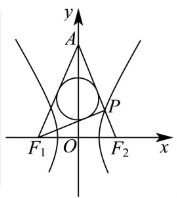
\includegraphics[width=0.2\linewidth]{bodyxb//src/37-3.png}
        \end{center}
        因为$\vv{P{F}_{1}} \cdot  \vv{P{F}_{2}} = 0$，所以$PF_1 \perp PF_2$，因此$\triangle PAF_1$是直角三角形，因此根据内切圆的性质可得$|PF_1|+|PA|-|AF_1| = 2r$，即$|PF_2|+2a+|PA|-|AF_1| = 2r$，即$|AF_2|-|AF_1| = 2r-2a$

        根据对称性可知$|AF_2|=|AF_1|$，因此$r = a = 2$

        \ps 本题若根据双曲线定义，对于焦点三角形$PF_1F_2$应用余弦定理（退化为勾股定理）得到$|PF_1|, |PF_2|$，再求$\triangle PAF_1$的三边后利用等面积法求内切圆半径也可，但计算量要大许多
    \end{jieda}
    \item 已知双曲线 ${\Gamma }_{1} : \dfrac{{x}^{2}}{{a}^{2}} - \dfrac{{y}^{2}}{{b}^{2}} = 1\left( {a > 0,b > 0}\right)$ 的左、右焦点分别为 ${F}_{1},{F}_{2}$ ,椭圆 ${\Gamma }_{2} : \dfrac{{x}^{2}}{3} + \dfrac{{y}^{2}}{4} =$ 1 的离心率为 $e$ ,直线 ${MN}$ 过点 ${F}_{2}$ 与双曲线交于 $M,N$ 两点,若 $\cos \angle {F}_{1}{MN} = \cos \angle {F}_{1}{F}_{2}M$ ,且 $\dfrac{\left| {F}_{1}M\right| }{\left| {F}_{1}N\right| } = e$ ,则双曲线 ${\Gamma }_{1}$ 的两条渐近线的倾斜角分别为\dotfill{(\kh{C})}
    \xx{${30}^{ \circ  },{150}^{ \circ  }$}{${45}^{ \circ  },{135}^{ \circ  }$}{${60}^{ \circ  },{120}^{ \circ  }$}{${15}^{ \circ  },{165}^{ \circ  }$}
    \begin{jieda}
        首先根据椭圆的标准方程可以算出$e = \dfrac{1}{2}$

        因为$\cos \angle {F}_{1}{MN} = \cos \angle {F}_{1}{F}_{2}M$，所以$\angle {F}_{1}{MN} = \angle {F}_{1}{F}_{2}M$，即$\triangle F_1F_2M$是等腰三角形，故$|F_1M| = |F_1F_2| = 2c$，因此$|F_1N| = 4c$，故可知$M,N$两点均在右支上.

        根据双曲线的定义可知$|F_2N| = 4c-2a$，$F_2M = 2c-2a$，因此可在$\triangle F_1F_2M$和$F_1F_2N$中利用余弦定理建立等式：$\dfrac{(2c)^2+(2c-2a)^2-(2c)^2}{2\times (2c) \times (2c-2a)} = -\left(\dfrac{(2c)^2+(4c-2a)^2-(4c)^2}{2\times (2c) \times (4c-2a)}\right)$，化简可得$3c^2+2a^2 = 7ac$，同除后解得$\dfrac{c}{a} = 2$，因此$\dfrac{b}{a} = \sqrt{3}$，故选$C$.
    \end{jieda}
    \item 已知双曲线 $\dfrac{{x}^{2}}{{a}^{2}} - {y}^{2} = 1\left( {a > 0}\right)$ ,点 $P\left( {{x}_{1},{y}_{1}}\right) \text{ 、 }Q\left( {{x}_{2},{y}_{2}}\right)$ 是右支上任意两点,且 ${x}_{1}{x}_{2} - {y}_{1}{y}_{2} > 0$ ,则 $a$ 的取值范围是\blkda{$[1, +\infty)$}.
    \begin{jieda}
        设$Q'(x_2, -y_2)$，则$Q'$也在右支上，因此命题可以转化为“点 $P\left( {{x}_{1},{y}_{1}}\right) \text{ 、 }Q\left( {{x}_{2},{y}_{2}}\right)$ 是右支上任意两点,且${x}_{1}{x}_{2} + {y}_{1}{y}_{2} > 0$”，即右支上任意两点和原点连线的夹角为锐角，因此边界情况是等轴双曲线，因此$a \in [1, +\infty)$满足题意.
    \end{jieda}
    \item 已知点 $A\left( {0,2}\right)$ ,抛物线 ${y}^{2} = {2px}\left( {p > 0}\right)$ 的焦点为 $F$ ,准线为 $l$ ,线段 ${FA}$ 交抛物线于点 $B$ , 过 $B$ 作准线 $l$ 的垂线,垂足为 $M$ ,若 ${AM}\bot {MF}$ ,则 $p =$ \blkda{$\sqrt{2}$}.
    \begin{jieda}
        因为${AM}\bot {MF}$，所以$\triangle AMF$为直角三角形

        根据抛物线的定义可知$|BM| = |BF|$，因此$B$是斜边中点，故$B\left(\dfrac{p}{4}, 1\right)$，代入抛物线方程可得$p = \sqrt{2}$
    \end{jieda}
    \item 如图, $\bigtriangleup {PAB}$ 所在的平面 $\alpha$ 和四边形 ${ABCD}$ 所在的平面 $\beta$ 互相垂直,且 ${AD} \bot  \alpha ,{BC} \bot  \alpha ,{AD} = 4,{BC} = 8,{AB} = 6$ . 若 $\tan \angle {ADP} - 2\tan \angle {BCP} = 1$ ,则动点 $P$ 在平面 $\alpha$ 内的轨迹是 \dotfill{(\kh{C})}
    
    \begin{center}
    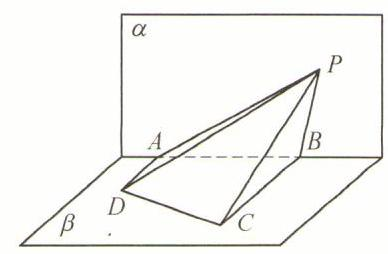
\includegraphics[width=0.3\textwidth]{bodyxb/src/bo_d1ig044601uc738hj6v0_78_1121_121_388_254_0.jpg}
    \end{center}
    \xx{椭圆的一部分}{线段}{双曲线的一部分}{以上都不是}
    \begin{jieda}
        $\left\{\begin{array}{l}
             \tan \angle {ADP} = \dfrac{AP}{AD} = \dfrac{AP}{4}  \\
             \tan \angle {BCP} = \dfrac{BP}{BC} = \dfrac{BP}{8}
        \end{array}\right.$，$\tan \angle {ADP} - 2\tan \angle {BCP} = 1$即$AP - BP = 4$，又因为$AB = 6 > 4$，因此选C.
    \end{jieda}
    \item 过双曲线 ${x}^{2} - \dfrac{{y}^{2}}{2} = 1$ 的右焦点作直线 $l$ 交双曲线于 $A\text{ 、 }B$ 两点,若实数 $\lambda$ 使得 $\left| {AB}\right|  = \lambda$ 的直线 $l$ 恰有 3 条,则 $\lambda  =$ \blkda{4}.
    \begin{jieda}
        通径长度为4，即两个交点都在右支上时，弦长最短为4；两个实轴距离为2，即交点左右两支各一个时，弦长最短为2；数形结合可知当$\lambda = 4$时满足要求.
    \end{jieda}
    \item 线段 ${AB}$ 两个端点均在抛物线 ${y}^{2} = {2x}$ 上,已知 $\left| {AB}\right|  = 3,M$ 是 ${AB}$ 的中点,那么 $M$ 到 $y$ 轴的最短距离是\blkda{1}.
    \begin{jieda}
        $x_M = \dfrac{x_A + x_B}{2} = \dfrac{\left(x_A+\dfrac{1}{2}\right) + \left(x_B+\dfrac{1}{2}\right)}{2} - \dfrac{1}{2} = \dfrac{|FA|+|FB|}{2} - \dfrac{1}{2} \geq \dfrac{|AB|}{2} - \dfrac{1}{2} = 1$（当$A,F,B$三点共线时取等号）
    \end{jieda}
    \item 抛物线 ${y}^{2} = {2px}\left( {p > 0}\right)$ 焦点为 $F$ ,准线为 $l.A,B$ 是抛物线上的两个动点,且满足 $\angle {AFB} = \dfrac{\pi }{3}$ . 设 ${AB}$ 中点 $M$ 在 $l$ 上的投影为 $N$ ,则 $\dfrac{\left| MN\right| }{\left| AB\right| }$ 的最大值是\blkda{1}.
    \begin{jieda}
        $|MN| = \dfrac{|FA| + |FB|}{2}$，根据余弦定理可知$ |AB|^2 = |FA|^2+|FB|^2 - |FA|\cdot|FB| = (|FA|+|FB|)^2 - 3|FA|\cdot|FB|$

        故$\dfrac{|MN|}{|AB|} = \dfrac{1}{2} \cdot \sqrt{\dfrac{(|FA| + |FB|)^2}{(|FA|+|FB|)^2 - 3|FA|\cdot|FB|}} \leq \dfrac{1}{2} \cdot \sqrt{\dfrac{(|FA| + |FB|)^2}{(|FA|+|FB|)^2 - 3\left(\dfrac{|FA|+|FB|}{2}\right)^2}} = 1$（当$|FA| = |FB|$时取等号）
    \end{jieda}
\end{enumerate}

\subsection*{38 离心率}

\subsubsection*{知识点睛}

离心率是描述圆锥曲线图形的重要参数, 在椭圆和双曲线中, 求解离心率本质是要寻找 $a$ , $b,c$ 三者或者其中两者的等式与不等式. 常见的处理方式有以下几种:

1. 常见的 $a,b,c$ 关系,比如渐近线与 $\dfrac{b}{a}$ ,焦半径,焦点弦,端点坐标,通径,最大张角等；

2. 将题设中的几何关系(中点,垂直,平行,特殊角,特殊图形等)转化为关于 $a,c$ 的关系;

3. 放在焦点三角形或者焦点弦三角形中,利用定义,结合正余弦定理、面积公式等寻找等量关系;

4. 将直线方程与圆锥曲线方程联立,利用判别式寻找 $a,c$ 的关系.

\subsubsection*{经典习题}

\begin{enumerate}
    \item 已知椭圆的中心在坐标原点,焦点在 $x$ 轴上, ${A}_{1},{A}_{2},{B}_{1},{B}_{2}$ 为椭圆顶点, ${F}_{2}$ 为右焦点,延长 ${B}_{1}{F}_{2}$ 与 ${A}_{2}{B}_{2}$ 交于点 $P$ ,若 $\angle {B}_{1}P{A}_{2}$ 为钝角,则该椭圆离心率的取值范围是\blkda[2]{$\left(\dfrac{\sqrt{5}-1}{2}, 1\right)$}.
    \begin{jieda}
        $\angle {B}_{1}P{A}_{2}$ 为钝角即$\vv{F_2B_1} \cdot \vv{B_2A_2} < 0$，$\vv{F_2B_1} = (-c, b), \vv{B_2A_2} = (a, b)$，故有$-ac+b^2<0$，即$e^2+e-1>0$

        结合离心率的定义可知$e \in \left(\dfrac{\sqrt{5}-1}{2}, 1\right)$
    \end{jieda}
    \item 已知两定点 $A\left( {-2,0}\right)$ 和 $B\left( {2,0}\right)$ ,动点 $P\left( {x,y}\right)$ 在直线 $l : y = x + 3$ 上移动,椭圆 $C$ 以 $A$ , $B$ 为焦点且经过点 $P$ ,则椭圆 $C$ 的离心率的最大值为\blkda{$\dfrac{2\sqrt{26}}{13}$}.
    \begin{jieda}
        焦点位置固定则$c$固定，当$a$取得最小值，即$b$取得最小值时离心率取得最大值，因此椭圆和直线$y = x + 3$的时候离心率取得最大值。

        设切点为$(x_0, y_0)$，则切线方程为$\dfrac{xx_0}{a^2}+\dfrac{yy_0}{b^2} = 1$，即$y = \dfrac{b^2}{y_0} - \dfrac{xx_0}{a^2} \cdot \dfrac{b^2}{y_0}$

        故有$\left\{\begin{array}{l}
             \dfrac{b^2}{y_0} = 3  \\
             \dfrac{x_0}{a^2} \cdot \dfrac{b^2}{y_0} = -1
        \end{array}\right.$，代入$\left\{\begin{array}{l}
             a^2 = b^2 + 4  \\
             y_0 = x_0 + 3
        \end{array}\right.$，可得$\dfrac{x_0}{a^2} \cdot \dfrac{b^2}{y_0} = -1$，化简可得$a^2 = \dfrac{13}{2}$，因此$e = \dfrac{2\sqrt{26}}{13}$
    \end{jieda}
    \item 设 ${F}_{1},{F}_{2}$ 为椭圆 $\dfrac{{x}^{2}}{{a}^{2}} + \dfrac{{y}^{2}}{{b}^{2}} = 1\left( {a > b > 0}\right)$ 的左、右焦点,且 $\left| {{F}_{1}{F}_{2}}\right|  = {2c}$ ,若椭圆上存在点 $P$ 使得 $\left| {P{F}_{1}}\right|  \cdot  \left| {P{F}_{2}}\right|  = 2{c}^{2}$ ,则椭圆的离心率的取值范围为\blkda{$\left[\dfrac{\sqrt{3}}{3}, \dfrac{\sqrt{2}}{2}\right]$}.
    \begin{jieda}
        设$t = |PF_1|$，则$t(2a-t) = 2c^2$在$[a-c, a+c]$内有解

        由于$y = -t^2+2at-2c^2$开口向下，对称轴为$t = a$，因此应有$\left\{\begin{array}{l}
             a(2a-a)-2c^2 \geq 0 \\
             (a+c)(2a-(a+c)) - 2c^2 \leq 0
        \end{array}\right.$，解得$e = \dfrac{c}{a} \in \left[\dfrac{\sqrt{3}}{3}, \dfrac{\sqrt{2}}{2}\right]$
    \end{jieda}
    \item 已知椭圆 $\dfrac{{x}^{2}}{{a}^{2}} + \dfrac{{y}^{2}}{{b}^{2}} = 1\left( {a > b > 0}\right)$ 上有一点 $A$ ,它关于原点的对称点为 $B$ ,点 $F$ 为椭圆的右焦点,且满足 ${AF} \bot  {BF}$ ,设 $\angle {ABF} = \alpha$ ,且 $\alpha  \in  \left\lbrack  {\dfrac{\pi }{12},\dfrac{\pi }{6}}\right\rbrack$ ,则该椭圆的离心率 $e$ 的取值范围为\blkda[3]{$\left[\sqrt{3}-1, \dfrac{\sqrt{6}}{3}\right]$}.
    \begin{jieda}
        易知$\triangle AFB$是直角三角，因此$OF$为斜边上的中线，因此$|AB| = 2c$，故$\left\{\begin{array}{l}
             |AF| = 2c \cdot  sin\alpha  \\
             |BF| = 2c \cdot  cos\alpha 
        \end{array} \right.$，故$2c(sin\alpha + cos\alpha) = 2a$，即$e = \dfrac{1}{sin\alpha + cos\alpha} = \dfrac{\sqrt{2}}{2sin\left(\alpha+\dfrac{\pi}{4}\right)}$
        
        因为$\alpha \in \left\lbrack  {\dfrac{\pi }{12},\dfrac{\pi }{6}}\right\rbrack$，所以$\alpha + \dfrac{\pi}{4} \in \left\lbrack  {\dfrac{\pi }{3},\dfrac{5\pi }{12}}\right\rbrack$，故$sin\left(\alpha+\dfrac{\pi}{4}\right) \in \left[\dfrac{\sqrt{3}}{2}, \dfrac{
        \sqrt{2}+\sqrt{6}}{2}\right]$，故$e \in \left[\sqrt{3}-1, \dfrac{\sqrt{6}}{3}\right]$
    \end{jieda}
    \item 已知 ${F}_{1},{F}_{2}$ 是双曲线 $\dfrac{{x}^{2}}{{a}^{2}} - \dfrac{{y}^{2}}{{b}^{2}} = 1\left( {a > 0,b > 0}\right)$ 的左、右两个焦点, $O$ 为双曲线的中心, 以线段 ${F}_{1}{F}_{2}$ 为直径的圆与双曲线的一条渐近线交于点 $M$ ,与双曲线交于点 $N$ (点 $M$ , $N$ 均在第一象限),当直线 $M{F}_{1}$ 与直线 ${ON}$ 平行时,双曲线离心率取值为 $e$ ,则 $e$ 所在区间为\dotfill{(\kh{A})}
    \xx{$\left( {1,\sqrt{2}}\right)$}{$\left( {\sqrt{2},\sqrt{3}}\right)$}{$\left( {\sqrt{3},2}\right)$}{$(2,3)$}
    \begin{jieda}
        易知$M(a, b)$，$F_1(-c, 0)$，设$N(x_0, y_0)$，则$\vv{F_1M} = (a+c, b), \vv{ON} = (x_0, y_0)$，根据两向量平行可知$bx_0 = (a+c)y_0$

        因为$\triangle NF_1F_2$为直角三角形，$ON$为斜边中线，因此有$x_0^2+y_0^2 = c^2$

        又因为$N$在双曲线上，因此有$\dfrac{{x_0}^{2}}{{a}^{2}} - \dfrac{{y_0}^{2}}{{b}^{2}} = 1$

        联立可得$\left\{\begin{array}{l}
             bx_0 = (a+c)y_0  \\
             x_0^2+y_0^2 = c^2 \\
             \dfrac{{x_0}^{2}}{{a}^{2}} - \dfrac{{y_0}^{2}}{{b}^{2}} = 1 \\
             a^2 + b^2 = c^2
        \end{array} \right.$，将第一个式子平方，将第三个式子去分母有$\left\{\begin{array}{l}
             b^2x_0^2 = (a+c)^2y_0^2  \\
             x_0^2+y_0^2 = c^2 \\
             b^2x_0^2 - a^2y_0^2 = a^2b^2 \\
             a^2 + b^2 = c^2
        \end{array} \right.$，消去$b^2$和$x_0^2$可得$\left\{\begin{array}{l}
             a^2(c^2-a^2) + a^2y_0^2 = (a+c)^2y_0^2  \\
             (c^2-a^2)(c^2- y_0^2) - a^2y_0^2 = a^2(c^2-a^2)
        \end{array} \right.$，即$\left\{\begin{array}{l}
             a^2c^2-a^4 = (c^2+2ac)y_0^2  \\
             c^4-y_0^2c^2 = 2a^2c^2-a^4 
        \end{array} \right.$，进一步消去$y_0^2$可得$\dfrac{a^2(c^2-a^2)}{c^2+2ac} = \dfrac{(c^2-a^2)^2}{c^2}$，即$\dfrac{a^2}{c^2+2ac} = \dfrac{c^2-a^2}{c^2}$，即$\dfrac{1}{e^2+2e} = \dfrac{e^2-1}{e^2}$，即$e = (e^2-1)(e+2)$，即$e^3+2e^2-2e-2 = 0$
        
        令$f(x) = x^3+2x^2-2x-2$，$f'(x) = 3x^2+4x-2$，故$f(x)$在$(1, +\infty)$严增，$f(1) = -1 < 0, f(\sqrt{2}) = 2 > 0$，因此选A.
    \end{jieda}
    \item 已知中心在坐标原点的椭圆和双曲线有公共焦点,且左、右焦点分别为 ${F}_{1},{F}_{2}$ ,这两条曲线在第一象限的交点为 $P,\bigtriangleup P{F}_{1}{F}_{2}$ 是以 $P{F}_{1}$ 为底边的等腰三角形. 若 $\left| {P{F}_{1}}\right|  = {10}$ ,椭圆与双曲线的离心率分别为 ${e}_{1},{e}_{2}$ ,则 ${e}_{1}{e}_{2}$ 的取值范围是\blkda{$\left(\dfrac{1}{3}, +\infty\right)$}.
    \begin{jieda}
        $|PF_2| = |F_1F_2| = 2c$，故有$\left\{\begin{array}{l}
             10 + 2c = 2a_1 \\
             10 - 2c = 2a_2 
        \end{array}\right.$
        
        $e_1e_2 = \dfrac{2c}{10+2c} \cdot \dfrac{2c}{10-2c} = \dfrac{4c^2}{100-4c^2} = \dfrac{1}{\dfrac{100}{4c^2} - 1}$

        根据双曲线定义和三角形两边之和大于第三边约束可知$2c \in (5, 10)$，因此$e_1e_2 \in \left(\dfrac{1}{3}, +\infty\right)$
    \end{jieda}
    \item 将离心率为 ${e}_{1}$ 的双曲线 ${C}_{1}$ 的实半轴长 $a$ 和虚半轴长 $b\left( {a \neq  b}\right)$ 同时增加 $m\left( {m > 0}\right)$ 个单位长度,得到离心率为 ${e}_{2}$ 的双曲线 ${C}_{2}$ ,则\dotfill{(\kh{D})}
    \xx{对任意的 $a,b,{e}_{1} > {e}_{2}$}{当 $a > b$ 时, ${e}_{1} > {e}_{2}$ ; 当 $a < b$ 时, ${e}_{1} < {e}_{2}$}{对任意的 $a,b,{e}_{1} < {e}_{2}$}{当 $a > b$ 时, ${e}_{1} < {e}_{2}$ ；当 $a < b$ 时, ${e}_{1} > {e}_{2}$}
    \begin{jieda}
        $e^2 = \dfrac{c^2}{a^2} = 1+ \dfrac{b^2}{a^2}$
    \end{jieda}
    \item 如图,在平面直角坐标系 ${xOy}$ 中, ${A}_{1},{A}_{2},{B}_{1},{B}_{2}$ 为椭圆 $\dfrac{{x}^{2}}{{a}^{2}} + \dfrac{{y}^{2}}{{b}^{2}} = 1\left( {a > b > 0}\right)$ 的四个顶点, $F$ 为其右焦点,直线 ${A}_{1}{B}_{2}$ 与直线 ${B}_{1}F$ 相交于点 $T$ ,线段 ${OT}$ 与椭圆的交点 $M$ 恰为线段 ${OT}$ 的中点,则该椭圆的离心率为\blkda{$2\sqrt{7}-5$}.
    
    \begin{center}
    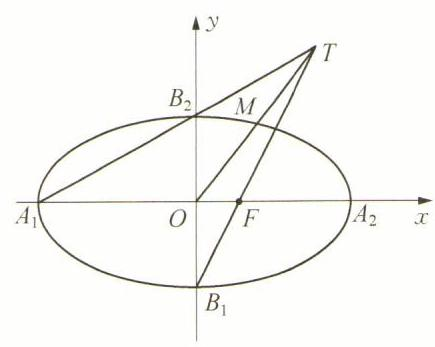
\includegraphics[width=0.3\textwidth]{bodyxb/src/bo_d1ig044601uc738hj6v0_80_1076_1003_435_347_0.jpg}
    \end{center}
    \begin{jieda}
        $A_1B_2: y = \dfrac{b}{a}x+b, B_1F: y = \dfrac{c}{b}x-b$

        联立，消去$y$得到$\dfrac{b}{a}x+b = \dfrac{b}{c}-b$，解得$x_T = \dfrac{2ac}{a-c}$，因此$T\left(\dfrac{2ac}{a-c}, \dfrac{b(a+c)}{a-c}\right)$，故$M\left(\dfrac{ac}{a-c}, \dfrac{b(a+c)}{2(a-c)}\right)$

        代入椭圆方程可得$\dfrac{1}{(a-c)^2}\left[c^2 + \dfrac{(a+c)^2}{4}\right] = 1$，即$e^2+10e-3=0$，解得$e = 2\sqrt{7}-5$
    \end{jieda}
    \item 已知双曲线 $\dfrac{{x}^{2}}{{a}^{2}} - \dfrac{{y}^{2}}{{b}^{2}} = 1\left( {a > 0,b > 0}\right)$ 的左、右焦点分别为 ${F}_{1}\left( {-c,0}\right) ,{F}_{2}\left( {c,0}\right)$ ,若双曲线上存在一点 $P$ 使 $\dfrac{\sin \angle P{F}_{1}{F}_{2}}{\sin \angle P{F}_{2}{F}_{1}} = \dfrac{a}{c}$ ,则该双曲线的离心率的取值范围是\blkda[2]{$(1, \sqrt{2}+1)$}.
    \begin{jieda}
        $\dfrac{\sin \angle P{F}_{1}{F}_{2}}{\sin \angle P{F}_{2}{F}_{1}} = \dfrac{|PF_2|}{|PF_1|}$，设$|PF_1| = t$，则存在$t$，使得$\dfrac{t-2a}{t} = \dfrac{a}{c}$，即$t = \dfrac{2ac}{c-a}$在$(a+c, +\infty)$有解

        故$\dfrac{2ac}{c-a} > a+c$，即$2e > e^2 - 1$，故$e \in (1, \sqrt{2}+1)$
    \end{jieda}
    \item 已知函数 $y = \dfrac{\sqrt{3}}{3}x - \dfrac{1}{x}$ 的图象是双曲线,那么该双曲线的离心率是\blkda{2}.
    \begin{jieda}
        对于双曲线的标准方程，设其渐近线的斜率为$k$，可知$k^2+1 = e^2$，因此两渐近线夹角的半角正切值的平方即$e^2-1$

        对于$y = \dfrac{\sqrt{3}}{3}x - \dfrac{1}{x}$，其两条渐近线分别是$y = \dfrac{\sqrt{3}}{3}x$和$y$轴，故其夹角为$\dfrac{2\pi}{3}$，因此$e=\sqrt{3+1} = 2$
    \end{jieda}
\end{enumerate}

\subsection*{39 点的存在性问题}

\subsubsection*{知识点睛}

在解决此类问题时, 常用的思路有以下几种:

1. 纯坐标运算, 两个相关点相互约束, 设坐标, 列等式, 再由表达式或者曲线的性质得出其中某个量的范围, 继而得到另一个量的范围;

2. 设动点坐标,利用条件求出所有满足要求的点的轨迹,再将点的存在性问题转化为曲线的交点问题,此方法非常实用,亦可解决点的个数问题；

3. 通过判断点在曲线上移动时,其所对应图形的角度、长度、面积等的变化规律,从而找到取得最值时的临界情况,再利用存在性问题的取最值的方法列不等式；

4. 这类问题一般都会涉及两到三个动点 (有可能更多), 这个时候往往需要用控制变量法 (主元法)研究在一个动点的情况下的变化情况,继而寻找最值或者范围.

\subsubsection*{经典习题}

\begin{enumerate}
    \item 已知曲线 $C : y =  - \sqrt{9 - {x}^{2}}$ ,直线 $l : y = 2$ ,若对于点 $A\left( {0,m}\right)$ ,存在 $C$ 上的点 $P$ 和 $l$ 上的点 $Q$ ,使得 $\vv{AP} + \vv{AQ} = \vv{0}$ ,则 $m$ 的取值范围是\blkda{$\left[-\dfrac{1}{2}, 1\right]$}.
    \begin{jieda}
        曲线$C$时以原点为圆心，3为半径的圆在$x$轴及其下方的部分，在其上任选一点$P(x, y)$，均存在$Q(-x, 2)$在直线$y = 2$上，$PQ$两者的中点$A(0, m)$在$y$轴上，满足$m = \dfrac{y+2}{2}$. 因为$y \in [-3, 0]$，因此$m \in \left[-\dfrac{1}{2}, 1\right]$
    \end{jieda}
    \item 在平面直角坐标系 ${xOy}$ 中,已知点 $A\left( {-2,0}\right)$ ,点 $B$ 是圆 $C : {\left( x - 2\right) }^{2} + {y}^{2} = 4$ 上的点,点 $M$ 为 ${AB}$ 中点,若直线 $l : y = {kx} - \sqrt{5}k$ 上存在点 $P$ ,使得 $\angle {OPM} = {30}^{ \circ  }$ ,则实数 $k$ 的取值范围为\blkda{$[-2, 2]$}.
    \begin{jieda}
        设$B(2+2cos\theta, 2sin\theta)$，则$M(cos\theta, sin\theta)$，因此$M$在以原点为圆心的单位圆上.

        对于直线上任意一点$P$，对于$\angle{OPM}$，当$M$为过$P$的单位圆的切线的切点时最大，当$M$为$OP$连线与单位圆交点时最小，因此要存在满足要求的点$P$，则应使得$\angle{OPM}$的最大值大于等于$\ang{30}$

        根据几何关系可知原点到直线$l$的距离应小于等于2，故$\dfrac{|\sqrt{5}k|}{\sqrt{1+k^2}} \leq 2$，解得$k \in [-2, 2]$
    \end{jieda}
    \item 设点 $M\left( {{x}_{0},1}\right)$ ,若在圆 $O : {x}^{2} + {y}^{2} = 1$ 上存在点 $N$ ,使得 $\angle {OMN} = {45}^{ \circ  }$ ,则 ${x}_{0}$ 的取值范围是\blkda{$[-1, 1]$}.
    \begin{jieda}
        对于$\angle{OMN}$，当$N$为过$M$的单位圆的切线的切点时最大，当$N$为$OM$连线与单位圆交点时最小，因此要存在满足要求的点$N$，则应使得$\angle{OMN}$的最大值大于等于$\ang{45}$

        根据几何关系已知$x_0 \in [-1, 1]$
    \end{jieda}
    \item 在平面直角坐标系 ${xOy}$ 中,圆 $C$ 的方程为 ${x}^{2} + {y}^{2} - {4x} = 0$ . 若直线 $y = k\left( {x + 1}\right)$ 上存在一点 $P$ ,使过 $P$ 所作的圆 $C$ 的两条切线相互垂直,则实数 $k$ 的取值范围是\blkda[2]{$[-2\sqrt{2}, 2\sqrt{2}]$}.
    \begin{jieda}
        设两切点为$Q_1, Q_2$，根据几何关系易知当$P$与圆心$C$的距离越近，则$\angle{Q_1PQ_2}$越大. 因此根据几何关系，要存在满足条件的$P$，则$C$到直线的距离应小于等于$2\sqrt{2}$，即$\dfrac{|3k|}{\sqrt{1+k^2}} \leq 2\sqrt{2}$，解得$k \in [-2\sqrt{2}, 2\sqrt{2}]$
    \end{jieda}
    \item 已知平面上两个点集 $M = \{ \left( {x,y}\right) \left| \right| x + y + 1\left| +\right| x + y - 1 \mid > 2,x \in  \mathbf{R},y \in  \mathbf{R}\} ,N =$  $\{ \left( {x,y}\right)  \mid  \left| {x - a}\right|  + \left| {y - 1}\right|  \leq  1,x \in  \mathbf{R},y \in  \mathbf{R}\}$ ,若 $M \cap  N = \varnothing$ ,则实数 $a$ 的取值集合是\blkda{$\{-1\}$}.
    \begin{jieda}
        根据三角不等式可知$\left| \right| x + y + 1\left| +\right| x + y - 1 \mid \geq 2$恒成立，当$x+y \in [-1, 1]$时取等号，因此$M$对应着平面上直线$x+y = 1$与直线$x+y = -1$所构成的条带以外的点（不含边界）

        集合$N$对应着以点$(a, 1)$为中心，$\sqrt{2}$为边长，对角线与坐标轴平行的的一个正方形区域

        根据图形可知，欲使两者交集为$\varnothing$，当且仅当$a = -1$
    \end{jieda}
    \item 在平面直角坐标系 ${xOy}$ 中,圆 ${C}_{1} : {\left( x + 1\right) }^{2} + {\left( y - 6\right) }^{2} = {25}$ ,圆 ${C}_{2} : {\left( x - {17}\right) }^{2} + {\left( y - {30}\right) }^{2} =$  ${r}^{2}$ . 若圆 ${C}_{2}$ 上存在一点 $P$ ,使得过点 $P$ 可作一条射线与圆 ${C}_{1}$ 依次交于点 $A,B$ ,满足 $\left| {PA}\right|  =$  $2\left| {AB}\right|$ ,则半径 $r$ 的取值范围是\blkda{$[5, 55]$}.
    \begin{jieda}
        数形结合，动态变化半径，从外离到内含
    \end{jieda}
    \item 圆 $C : {\left( x - 2\right) }^{2} + {y}^{2} = 1$ 上存在点 $P$ 满足: $P$ 到原点的距离与 $P$ 到直线 $l : y = {kx}$ 的距离之比为 $\sqrt{2}$ ,则 $k$ 的取值范围为\blkda[6]{$[-2-\sqrt{3}, -2+\sqrt{3}] \cup [2-\sqrt{3}, 2+\sqrt{3}]$}.
    \begin{jieda}
        因为$y = kx$过原点，因此满足$P$ 到原点的距离与 $P$ 到直线 $l : y = {kx}$ 的距离之比为 $\sqrt{2}$的点$P$应在过原点，与$l$夹角为$\ang{45}$的两条直线$l_1, l_2$上，因此要使得圆 $C : {\left( x - 2\right) }^{2} + {y}^{2} = 1$ 上存在点 $P$，则应使得$l_1, l_2$之一和圆有交点

        数形结合可知直线$l$的倾斜角$\theta$应满足$\ang{15} \leq \theta \leq \ang{75}$或$\ang{115} \leq \theta \leq \ang{175}$，因此$k = \tan\theta \in [-2-\sqrt{3}, -2+\sqrt{3}] \cup [2-\sqrt{3}, 2+\sqrt{3}]$
    \end{jieda}
    \item 已知平面直角坐标系中的直线 ${l}_{1} : y = {2x},{l}_{2} : y =  - {2x}$ ,设到 ${l}_{1}\text{ 、 }{l}_{2}$ 距离之和为 $2{c}_{1}$ 的点的轨迹是曲线 ${C}_{1}$ ,到 ${l}_{1}$ 、 ${l}_{2}$ 距离平方和为 $2{c}_{2}$ 的点的轨迹是曲线 ${C}_{2}$ ,其中 ${c}_{1}\text{ 、 }{c}_{2} > 0$ ,则 ${C}_{1}$ 、 ${C}_{2}$ 公共点的个数不可能为 \dotfill{(\kh{D})}
    \xx{0 个}{4 个}{8 个}{12 个}
    \begin{jieda}
        设曲线 ${C}_{1}$上的点为$(x,y)$，满足 $\dfrac{\left| 2x - y\right| }{\sqrt{5}} + \dfrac{\left| 2x + y\right| }{\sqrt{5}} = 2{c}_{1}$ ,即
        $\left| {{2x} - y}\right|  + \left| {{2x} + y}\right|  = 2\sqrt{5}{c}_{1}$
        \begin{dingautolist}{172}
            \item 当 ${2x} - y > 0$ , ${2x} + y > 0$ 时, $x = \dfrac{\sqrt{5}}{2}{c}_{1}$
            \item ${2x} - y > 0$ , ${2x} + y < 0$ 时, $y =  - \sqrt{5}{c}_{1}$
            \item ${2x} - y < 0$ , ${2x} + y > 0$ 时, $y = \sqrt{5}{c}_{1}$
            \item ${2x} - y < 0$ , ${2x} + y < 0$ 时, $x =  - \dfrac{\sqrt{5}}{2}{c}_{1}$ 
        \end{dingautolist}
        所以曲线 ${C}_{1}$ 是以 $\left( {\dfrac{\sqrt{5}}{2}{c}_{1},\sqrt{5}{c}_{1}}\right)$ 、
        $\left( {-\dfrac{\sqrt{5}}{2}{c}_{1},\sqrt{5}{c}_{1}}\right) \text{、}\left( {-\dfrac{\sqrt{5}}{2}{c}_{1}, - \sqrt{5}{c}_{1}}\right)$ 、
        $\left( {\dfrac{\sqrt{5}}{2}{c}_{1}, - \sqrt{5}{c}_{1}}\right)$ 为顶点的矩形
        
        设曲线 ${C}_{2}$ 上的点为 $\left( {{x}^{\prime },{y}^{\prime }}\right)$ ,满足
        ${\left( \dfrac{\left| 2{x}^{\prime } - {y}^{\prime }\right| }{\sqrt{5}}\right) }^{2} + {\left( \dfrac{\left| 2{x}^{\prime } + {y}^{\prime }\right| }{\sqrt{5}}\right) }^{2} = 2{c}_{2}$ ,即
        ${x}^{\prime 2} + \dfrac{{y}^{\prime 2}}{4} = \dfrac{5}{4}{c}_{2}$
        所以 ${C}_{2}$ 是椭圆 ${x}^{2} + \dfrac{{y}^{2}}{4} = \dfrac{5}{4}{c}_{2}$ 

        因此两者的公共点个数只能是0、4、8个.
    \end{jieda}
    \item 在平面直角坐标系 ${xOy}$ 中,已知直线 $l : y = {kx} + 6$ 上存在点 $P$ ,过点 $P$ 作圆 $O : {x}^{2} + {y}^{2} =$ 4 的切线,切点分别为 $A\left( {{x}_{1},{y}_{1}}\right)$ 、 $B\left( {{x}_{2},{y}_{2}}\right)$ ,且 ${x}_{1}{x}_{2} + {y}_{1}{y}_{2} =  - 2$ ,则实数 $k$ 的取值范围为\blkda[5]{$\left(-\infty, -\dfrac{\sqrt{5}}{2}\right] \cup \left[\dfrac{\sqrt{5}}{2}, +\infty\right)$}.
    \begin{jieda}
        设$\theta = \angle{AOB}$，则${x}_{1}{x}_{2} + {y}_{1}{y}_{2} = 4cos\theta = -2$，因此$cos\theta = -\dfrac{1}{2}$，$\theta = \dfrac{2\pi}{3}$，因此$\angle{APB} = \dfrac{\pi}{3}$

        故$|PO| = 4$，因此$l$到原点的距离小于等于4，即$\dfrac{6}{\sqrt{1+k^2}} \leq 4$，解得$k \in \left(-\infty, -\dfrac{\sqrt{5}}{2}\right] \cup \left[\dfrac{\sqrt{5}}{2}, +\infty\right)$
    \end{jieda}
    \item 在平面直角坐标系 ${xOy}$ 中,圆 $O : {x}^{2} + {y}^{2} = 1$ ,圆 $M : {\left( x + a + 3\right) }^{2} + {\left( y - 2a\right) }^{2} = 1(a$ 为实数),若圆 $O$ 与圆 $M$ 上分别存在点 $P\text{ 、 }Q$ ,使得 $\angle {OQP} = {30}^{ \circ  }$ ,则实数 $a$ 的取值范围是\blkda{$\left[-\dfrac{6}{5}, 0\right]$}.
    \begin{jieda}
        对于任意一点$Q$，对于$\angle{OQP}$，当$P$为过$Q$的单位圆的切线的切点时最大，当$P$为$OQ$连线与单位圆交点时最小，因此要存在满足要求的点$Q$，则应使得$\angle{OQP}$的最大值大于等于$\ang{30}$，即$OQ$距离小于等于$2$，即$OM$距离小于等于$3$

        $M$在直线$y = -2x-6$上，故$x_M \in \left[-3, -\dfrac{9}{5}\right]$时满足要求，因此$a \in \left[-\dfrac{6}{5}, 0\right]$
    \end{jieda}
\end{enumerate}

\subsection*{40 位置关系}

\subsubsection*{知识点睛}

1. 直线与圆、圆锥曲线有三种位置关系,包括相离、相切和相交. 直线与圆的位置关系一般用半径和圆心到直线的距离做比较. 直线与椭圆、双曲线、抛物线的位置关系一般需联立方程判断交点个数,继而判断位置关系；

2. 圆锥曲线通用的弦长公式是 $l = \sqrt{1 + {k}^{2}}\left| {{x}_{1} - {x}_{2}}\right|  = \sqrt{1 + {k}^{2}}\dfrac{\sqrt{\Delta }}{\left| A\right| }$ ,其中 $k$ 是弦所在直线的斜率, ${x}_{1},{x}_{2}$ 是直线与圆锥曲线联立得到的方程 $A{x}^{2} + {Bx} + C = 0\left( {A \neq  0}\right)$ 的两根, $\Delta$ 是这一方程的判别式, $A$ 是其二次项系数;

3. 直线与椭圆、双曲线、抛物线相切时,一般会联立方程,取 $\Delta  = 0$ 来求解参数. 事实上, ${Ax} + {By} + C = 0$ 与 $\dfrac{{x}^{2}}{{a}^{2}} \pm  \dfrac{{y}^{2}}{{b}^{2}} = 1$ 相切的充要条件是 ${a}^{2}{A}^{2} \pm  {b}^{2}{B}^{2} = {C}^{2}$ ;

4. 以曲线 $A{x}^{2} + B{y}^{2} + {Dx} + {Ey} + F = 0$ 上一点 $P\left( {{x}_{0},{y}_{0}}\right)$ 为切点的切线方程为 $A{x}_{0}x +$  $B{y}_{0}y + D \cdot  \dfrac{{x}_{0} + x}{2} + E \cdot  \dfrac{{y}_{0} + y}{2} + F = 0$ . 特别地,圆方程为 ${\left( x - a\right) }^{2} + {\left( y - b\right) }^{2} = {r}^{2}$ 时,切线方程为 $\left( {x - a}\right) \left( {{x}_{0} - a}\right)  + \left( {y - b}\right) \left( {{y}_{0} - b}\right)  = {r}^{2}$ ,当 $P$ 为曲线外一点时,该方程为切点弦所在直线方程.

\subsubsection*{经典习题}
\begin{enumerate}
    \item 动圆 $C$ 经过点 $F\left( {1,0}\right)$ ,并且与直线 $x =  - 1$ 相切,若动圆 $C$ 与直线 $y = x + 2\sqrt{2} + 1$ 总有公共点,则圆 $C$ 的面积\dotfill{(\kh{D})}
    \xx{有最大值 ${8\pi }$}{有最小值 ${2\pi }$}{有最小值 ${3\pi }$}{有最小值 ${4\pi }$}
    \begin{jieda}
        根据题意易知动圆 $C$的圆心位于抛物线$y^2 = 4x$上，设圆心为$\left(\dfrac{b^2}{4}, b\right)$
        
        若动圆 $C$ 与直线 $y = x + 2\sqrt{2} + 1$ 总有公共点，则圆心到直线的距离应大于等于动圆 $C$ 的半径，即$\dfrac{\left|\dfrac{b^2}{4} - b+2\sqrt{2}+1\right|}{\sqrt{2}} \leq \left(\dfrac{b^2}{4}+1\right)$

        易知$\Delta = 1 - (2\sqrt{2}+1) < 0$，故不等式可以转化为$\dfrac{b^2}{4} - b+2\sqrt{2}+1 \leq \sqrt{2}\left(\dfrac{b^2}{4}+1\right)$，进一步化简有$\dfrac{(\sqrt{2}-1)b^2}{4}+b-\sqrt{2} -1 \geq 0$解得$b \in (-\infty, -(6+4\sqrt{2})] \cup [2, +\infty)$

        而动圆$C$的面积为$\left(\dfrac{b^2}{4}+1\right)^2\pi$，故其最小值为$4\pi$，当$b = 2$时取得最小值.
    \end{jieda}
    \item 直线 ${l}_{1} : y = x + a$ 和 ${l}_{2} : y = x + b$ 将单位圆 $C : {x}^{2} + {y}^{2} = 1$ 分成长度相等的四段弧,则 ${a}^{2} +$  ${b}^{2} =$ \blkda{2}.
    \begin{jieda}
        数形结合可知$a = 1$，$b = -1$或对称情况.
    \end{jieda}
    \item 已知点 $E$ 是抛物线 $C : {y}^{2} = {2px}\left( {p > 0}\right)$ 的对称轴与准线的交点,点 $F$ 为抛物线 $C$ 的焦点, 点 $P$ 在抛物线 $C$ 上,在 $\bigtriangleup {EFP}$ 中,若 $\sin \angle {EFP} = \mu  \cdot  \sin \angle {FEP}$ ,则 $\mu$ 的最大值为\blkda{$\sqrt{2}$}.
    \begin{jieda}
        $\mu = \dfrac{sin\angle{EFP}}{sin\angle{FEP}} = \dfrac{|EP|}{|FP|} = \dfrac{|EP|}{|PH|} = \dfrac{1}{sin\angle{PEH}}$，其中$H$是过$P$做准线的垂线的垂足

        因此当$P$为过$E$与抛物线相切的切点时，$\mu$最大，设$P(x_0, y_0)$，切线为$y = \dfrac{y_0}{2x_0}x+\dfrac{y_0}{2}$，令其过$E\left(-\dfrac{p}{2}, 0\right)$，可得$P\left(\dfrac{p}{2}, p\right)$，因此$\mu = \sqrt{2}$
    \end{jieda}
    \item 设直线 $l$ 与抛物线 ${y}^{2} = {4x}$ 相交于 $A\text{ 、 }B$ 两点,与圆 ${\left( x - 5\right) }^{2} + {y}^{2} = {r}^{2}\left( {r > 0}\right)$ 相切于点 $M$ , 且 $M$ 为线段 ${AB}$ 的中点,若这样的直线 $l$ 恰有 4 条,则 $r$ 的取值范围是\blkda{$(2, 4)$}.
    \begin{jieda}
        数形结合可知有两条切线为垂直于$x$轴的切线

        设斜率存在时$M(x_0, y_0)$，因此对应的切线$AB$为$(x-5)(x_0 - 5)+yy_0 = r^2$，设$A(x_1, y_1), B(x_2, y_2)$，则有$\left\{\begin{array}{l}
             y_1^2 = 4x_1 \\
             y_2^2 = 4x_2
        \end{array}\right.$，两者作差有$(y_1^2 - y_2^2) = 4(x_1-x_2)$即$(y_1+y_2)(y_1 - y_2) = 4(x_1-x_2)$，故$k_{AB} = \dfrac{4}{y_1+y_2} = \dfrac{2}{y_0}$，根据方程$(x-5)(x_0 - 5)+yy_0 = r^2$可知$k_{AB} = \dfrac{5-x_0}{y_0}$，因此$x_0 = 3$

        故当圆上存在横坐标为$3$的点时会出现另外两条切线，但根据图象可知圆上横坐标为$3$的点应在抛物线内部才可以，即$r \in (2, 4)$
    \end{jieda}
    \item 已知曲线 ${C}_{1} : y = {x}^{2} + 4$ 和 ${C}_{2} : y = {2x} - {x}^{2}$ ,直线 ${l}_{1}$ 与 ${C}_{1}\text{ 、 }{C}_{2}$ 分别相切于 $A\text{ 、 }B$ ,直线 ${l}_{2}$ (不同于 ${l}_{1}$ )与 ${C}_{1}$ 、 ${C}_{2}$ 分别相切于点 $C$ 、 $D$ ,则 ${AB}$ 与 ${CD}$ 交点的横坐标是\blkda{$\dfrac{1}{2}$}.
    \begin{jieda}
        $C_2: y = -(x-1)^2+1$，故$C_1, C_2$开口大小相同，存在对称中心$\left(\dfrac{1}{2}, \dfrac{5}{2}\right)$，公切线的交点应该是对称中心，此时两切线也各自关于该点中心对称.
    \end{jieda}
    \item 若 $P$ 是双曲线 $C : \dfrac{{x}^{2}}{{a}^{2}} - \dfrac{{y}^{2}}{{b}^{2}} = 1\left( {a > 0,b > 0}\right)$ 的渐近线上任意一点,下列正确的是\dotfill{(\kh{C})}
    \xx{存在过点 $P$ 的直线与该双曲线相切}{不存在过点 $P$ 的直线与该双曲线相切}{至多存在一条过点 $P$ 的直线与该双曲线相切}{至多存在一条过点 $P$ 的直线与该双曲线只有一个交点}
    \begin{jieda}
        当$P$为原点的时候，不存在切线，否则至多存在一条切线
    \end{jieda}
    \item 已知直线 $y = k\left( {x - m}\right)$ 与抛物线 ${y}^{2} = {2px}\left( {p > 0}\right)$ 交于 $A,B$ 两点, $O$ 为坐标原点,且 ${OA} \bot  {OB}$ ,又 ${OD} \bot  {AB}$ 于 $D$ ,若动点 $D$ 的坐标满足方程 ${x}^{2} + {y}^{2} - {4x} = 0$ ,则 $p = $ \blkda{2}.
    \begin{jieda}
        考虑特殊情况，当$AB$垂直于$x$轴时，要满足$OA \perp OB$，则应有$x_A = x_B = 2p$，此时$D(2p, 0)$，而${x}^{2} + {y}^{2} - {4x} = 0$与$x$轴的交点为$(0, 0)$和$(4,0)$，显然前者不符合要求，因此$p = 2$

        经检验$p = 2, m = 4$满足要求.
    \end{jieda}
    \item 过抛物线 ${y}^{2} = {4x}$ 的焦点作一条倾斜角为 $\alpha$ ,长度不超过 8 的弦,弦所在的直线与圆 ${x}^{2} +$  ${y}^{2} = \dfrac{3}{4}$ 有公共点,则 $\alpha$ 的取值范围是\blkda[3]{$\left[\dfrac{\pi}{4}, \dfrac{\pi}{3}\right] \cup \left[\dfrac{2\pi}{3}, \dfrac{3\pi}{4}\right]$}.
    \begin{jieda}
        设弦所在直线为$y = k(x-1)$
        \begin{dingautolist}{172}
            \item 欲使弦与圆${x}^{2} +$  ${y}^{2} = \dfrac{3}{4}$ 有公共点，则原点到弦的距离应当小于等于半径，即$\dfrac{|k|}{\sqrt{1+k^2}} \leq \dfrac{\sqrt{3}}{2}$，故$k \in [-\sqrt{3}, \sqrt{3}]$

            \item $|AB| = \dfrac{2p}{sin^2\alpha} = \dfrac{4}{sin^2\alpha} \leq 8$，故$sin^2\alpha \geq \dfrac{1}{2}$，即$k^2 \geq 1$
        \end{dingautolist}
        综上，$k \in [-\sqrt{3}, -1] \cup [1, \sqrt{3}]$，因此$\alpha \in \left[\dfrac{\pi}{4}, \dfrac{\pi}{3}\right] \cup \left[\dfrac{2\pi}{3}, \dfrac{3\pi}{4}\right]$
    \end{jieda}
    \item 如图, $F$ 为椭圆 $\dfrac{{x}^{2}}{5} + {y}^{2} = 1$ 的右焦点,第一象限内的点 $M$ 在椭圆上,若 ${MF} \bot  x$ 轴,直线 ${MN}$ 与圆 ${x}^{2} + {y}^{2} = 1$ 相切于第四象限内的点 $N$ ,则 $\left| {NF}\right|$ 等于\blkda{$\dfrac{\sqrt{21}}{3}$}.
    
    \begin{center}
    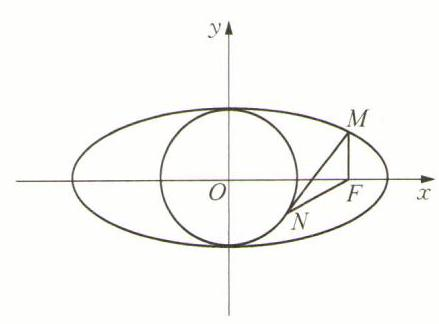
\includegraphics[width=0.3\textwidth]{bodyxb/src/bo_d1ig044601uc738hj6v0_84_1067_1036_439_324_0.jpg}
    \end{center}
    \begin{jieda}
        $F(2, 0), M\left(2, \dfrac{\sqrt{5}}{5}\right)$，设 ${l}_{MN} : y - \dfrac{\sqrt{5}}{5}= k\left( {x - 2}\right)$ ,
        $N\left( {x,y}\right)$ ,则 $O$ 到 ${l}_{MN}$ 的距离 $d = \dfrac{\left| -2k + \dfrac{\sqrt{5}}{5}\right| }{\sqrt{{k}^{2} + 1}} = 1$ ,解得 $k = \dfrac{2\sqrt{5}}{5}$ (负
        值舍去).
        又因为 $\left\{  \begin{array}{l} {x}^{2} + {y}^{2} = 1, \\  y - \dfrac{\sqrt{5}}{5} = \dfrac{2\sqrt{5}}{5}\left( {x - 2}\right)  \end{array}\right.$
        $\Longrightarrow  \left\{  \begin{array}{l} x = \dfrac{2}{3}, \\  y =  - \dfrac{\sqrt{5}}{3}, \end{array}\right.$
        即 $N\left( {\dfrac{2}{3}, - \dfrac{\sqrt{5}}{3}}\right)$ ,所以 $|{NF}|= \sqrt{{\left( 2 - \dfrac{2}{3}\right) }^{2} + {\left( \dfrac{\sqrt{5}}{3}\right) }^{2}} = \dfrac{\sqrt{21}}{3}$
    \end{jieda}

    \item 若圆与抛物线有公共点 $A$ ,且以 $A$ 为切点的两条切线重合,我们就称圆与抛物线是 “相切”的, $A$ 称为 “公切点”. 已知圆 ${\left( x - a\right) }^{2} + {y}^{2} = {a}^{2}$ 与 ${y}^{2} = {4x}$ 恰有 $n$ 个“公切点”,那么 $n$ 的取值可能是\blkda{1}.
    \begin{jieda}
        联立圆和抛物线的方程，$\left\{\begin{array}{l}
             {y}^{2} = {4x}  \\
             {\left( x - a\right) }^{2} + {y}^{2} = {a}^{2}
        \end{array}\right.$，消去$y$得到${\left( x - a\right) }^{2} + 4x = {a}^{2}$，化简得到$x(x-(2a-4)) = 0$
        \begin{dingautolist}{172}
            \item 已知$x = 0$时满足题意
            \item 当$x = 2a-4(a>2)$时，圆的切线为$(x-a)(a-4)+y(\sqrt{8a-16}) = a^2$和$(x-a)(a-4)-y(\sqrt{8a-16}) = a^2$，抛物线的切线为$y(\sqrt{8a-16}) = 2(x+(2a-4))$或$-y(\sqrt{8a-16}) = 2(x+(2a-4))$

            显然相同切点对应的切线斜率不同，不符合要求
        \end{dingautolist}
    \end{jieda}
\end{enumerate}

\subsection*{41 对称与旋转问题}

\subsubsection*{知识点睛}

对称包括中心对称和轴对称,我们需要掌握常见的点的中心对称和轴对称问题的解决方案. $A\text{ 、 }B$ 关于 $C$ 对称,则有 $C$ 是线段 ${AB}$ 中点; $A\text{ 、 }B$ 关于 $l$ 对称,则 ${AB}\bot l$ ,且 ${AB}$ 中点在 $l$ 上.

线是由点组成的,所以曲线的对称与旋转问题本质上是将曲线上所有的点做相同的变换, 既可以设点坐标,进行变换后得到新的点坐标,再由相关点法求曲线方程,也可以将曲线看作点的轨迹, 从而点的变换可以看作曲线的变换, 得到新的曲线.

曲线在旋转以及对称变化前后,曲线的形状不会发生变化,改变的是位置和角度, 我们经常会将这种非标准方程的圆锥曲线变换成标准方程,从而研究圆锥曲线的各种参数.

\subsubsection*{经典习题}
\begin{enumerate}
    \item 对于任意放置的椭圆,经过椭圆上的任意一点有且仅有一直线与该椭圆有一个交点,则称该直线为椭圆的切线. 椭圆 $\dfrac{{x}^{2}}{2} + {y}^{2} = 1$ 绕坐标原点逆时针旋转 ${45}^{ \circ  }$ 后得到的椭圆中最高点与原点的距离为\blkda{$\dfrac{\sqrt{15}}{3}$}.
    \begin{jieda}
        易知旋转后的最高点即旋转前斜率为$-1$的切线在第一象限的切点，故设切线方程为$x+y = m (m > 0)$，所求距离即切点到原点的距离.

        联立切线方程与椭圆方程有$\left\{\begin{array}{l}
             x+y = m \\
             \dfrac{{x}^{2}}{2} + {y}^{2} = 1
        \end{array}\right.$，消去$y$得到$\dfrac{3}{2}x^2-2mx+m^2-1 = 0$，$\Delta = 4m^2 - 6(m^2-1) = 0$，故$m = \sqrt{3}$

        因此切线方程为$x+y = \sqrt{3}$，设切点为$(x_0, y_0)$，则切线方程为$\dfrac{x_0x}{2}+y_0y = 1$，方程两侧同时乘$\sqrt{3}$，令对应系数相等可得$\left\{\begin{array}{l}
             x_0 = \dfrac{2\sqrt{3}}{3} \\
             y_0 = \dfrac{\sqrt{3}}{3}
        \end{array}\right.$，故切点到原点距离为$\sqrt{\dfrac{1}{3}+\dfrac{4}{3}} = \dfrac{\sqrt{15}}{3}$
    \end{jieda}
    \item 已知圆 ${x}^{2} + {y}^{2} + {2x} - {4y} + a = 0$ 关于直线 $y = {2x} + b$ 成轴对称,则 $a - b$ 的取值范围是\blkda{$(-\infty, 1)$}.
    \begin{jieda}
        因为对称轴会过圆心，所以$y = {2x} + b$过$(-1, 2)$，因此$b = 4$，而${x}^{2} + {y}^{2} + {2x} - {4y} + a = 0$表示圆则要求$5-a > 0$，即$a \in (-\infty, 5)$

        故$a - b \in (-\infty, 1)$
    \end{jieda}
    \item 若双曲线 $\dfrac{{x}^{2}}{{a}^{2}} - \dfrac{{y}^{2}}{{b}^{2}} = 1\left( {a > 0,b > 0}\right)$ 上不存在点 $P$ 使得右焦点 $F$ 关于直线 ${OP}(O$ 为双曲线的中心)的对称点在 $y$ 轴上,则该双曲线离心率的取值范围为\blkda{$(1, \sqrt{2}]$}.
    \begin{jieda}
        若右焦点 $F$ 关于直线 ${OP}(O$ 为双曲线的中心)的对称点在 $y$ 轴上，则直线$OP$必定为$y = x$或$y = -x$
        
        因为双曲线上不存在这样的$P$点，所以这两条直线与双曲线没有交点，因此$\dfrac{b}{a} \leq 1$，故$e \in (1, \sqrt{2}]$
    \end{jieda}
    \item 已知抛物线 $y =  - {x}^{2} + 3$ 上存在关于直线 $x + y = 0$ 对称的相异两点 $A\text{ 、 }B$ ,则 $\left| {AB}\right|$ 等于\blkda{$3\sqrt{2}$}.
    \begin{jieda}
        因为$A\text{ 、 }B$关于直线 $x + y = 0$ 对称，所以直线$AB$可以设为$y = x + m$，联立直线和抛物线方程可得$\left\{\begin{array}{l}
             y = x + m \\
             y = -x^2 + 3
        \end{array}\right.$，消去$y$可得$x^2 + x + m - 3 = 0$，因此$AB$中点为$\left(-\dfrac{1}{2}, m-\dfrac{1}{2}\right)$，因为中点在$x+y=0$上，所以$m = 1$，故$|AB| = \sqrt{2}|x_1-x_2| = 3\sqrt{2}$
    \end{jieda}
    \item 若抛物线 $y = a{x}^{2} - 1$ 上总存在两点关于直线 $x + y = 0$ 对称,则实数 $a$ 的取值范围是\blkda{$\left(\dfrac{3}{4}, +\infty\right)$}.
    \begin{jieda}
        设抛物线上$A\text{ 、 }B$两点关于直线 $x + y = 0$ 对称，则直线$AB$可以设为$y = x + m$，联立直线和抛物线方程可得$\left\{\begin{array}{l}
             y = x + m \\
             y = ax^2 - 1
        \end{array}\right.$，消去$y$可得$x + m = ax^2 - 1$，即$ax^2-x-(m+1) = 0$

        首先应满足$\Delta = 1+4a(m+1) > 0$，其次根据韦达定理$AB$中点坐标为$\left(\dfrac{1}{2a}, m+\dfrac{1}{2a}\right)$，因为中点在$x+y=0$上，所以$m + \dfrac{1}{a} = 0$，代入$\Delta = 1+4a(m+1) > 0$可得$1 - 4 + 4a > 0$，因此$a > \dfrac{3}{4}$
    \end{jieda}
    \item 如果椭圆 $\dfrac{{x}^{2}}{{a}^{2}} + \dfrac{{y}^{2}}{{b}^{2}} = 1\left( {a > b > 0}\right)$ 的右焦点 (1,0) 关于直线 $y = {bx}$ 的对称点在椭圆上,则 $a =$ \blkda{$\sqrt{2}$}.
    \begin{jieda}
        \begin{enumerate}
            \item 方法1 \\
            设$b = tan\theta, \theta \in \left(0, \dfrac{\pi}{2}\right)$，则$(1, 0)$关于$y = bx$的对称点为$(cos2\theta, sin2\theta)$，代入椭圆方程可得$\dfrac{cos^2(2\theta)}{1+tan^2\theta} + \dfrac{sin^2(2\theta)}{tan^2\theta} = 1$，即$cos^2(2\theta) \cdot cos^2\theta + 4cos^4\theta = 1$，即$cos^2\theta[4cos^4\theta+1] = 1$

            换元$t = cos^2\theta, t \in (0, 1)$，故$4t^2+1 = \dfrac{1}{t}$，数形结合可以判断关于$t$的方程只有一解，观察可知$t = \dfrac{1}{2}$满足要求，因此$\theta = \dfrac{\pi}{4}$
            
            故$b = 1$，因此$a = \sqrt{2}$
            \item 方法2 \\
            设右焦点(1,0)关于直线 $y = {bx}$的对称点的坐标为 $\left( {{x}_{0},{y}_{0}}\right)$ . 
            
            由题意可得
            $\left\{  {\begin{array}{l} \dfrac{0 + {y}_{0}}{2} = b \cdot  \dfrac{1 + {x}_{0}}{2} \\  \dfrac{{y}_{0}}{{x}_{0} - 1} =  - \dfrac{1}{b} \end{array}\text{,得}\left\{  {\begin{array}{l} {x}_{0} = \dfrac{1 - {b}^{2}}{1 + {b}^{2}} \\  {y}_{0} = \dfrac{2b}{1 + {b}^{2}} \end{array}\text{. 又}\left( {{x}_{0},{y}_{0}}\right)}\right. }\right.$
            在椭圆上, $\therefore \dfrac{{x}_{0}^{2}}{{a}^{2}} + \dfrac{{y}_{0}^{2}}{{b}^{2}} = 1$ ,即 $\dfrac{{\left( \dfrac{1 - {b}^{2}}{1 + {b}^{2}}\right) }^{2}}{{a}^{2}} + \dfrac{{\left( \dfrac{2b}{1 + {b}^{2}}\right) }^{2}}{{b}^{2}} =$
            1. 又 ${a}^{2} = {b}^{2} + {c}^{2} = {b}^{2} + 1$ ,解得 ${a}^{2} = 2$ ,即 $a = \sqrt{2}$ .
        \end{enumerate}
    \end{jieda}
    \item 设圆 $O$ 的半径为 2,点 $P$ 为圆周上给定一点,如图,放置边长为 2 的正方形 ${ABCD}$ (实线所示,正方形的顶点 $A$ 与点 $P$ 重合,点 $B$ 在圆周上),现将正方形 ${ABCD}$ 沿圆周按顺时针方向连续滚动,当点 $A$ 首次回到点 $P$ 的位置时,点 $A$ 所走过的路径的长度为\blkda{$(2 + \sqrt{2})\pi$}.
    
    \begin{center}
    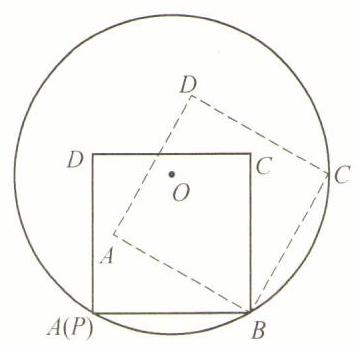
\includegraphics[width=0.3\textwidth]{bodyxb/src/bo_d1ig044601uc738hj6v0_86_1154_125_357_349_0.jpg}
    \end{center}
    \begin{jieda}
        以正方形的边为弦时,该弦所对的圆心角为 $\dfrac{\pi }{3}$ ,正方形在圆周上滚动时点的顺序如图所示
        \begin{center}
            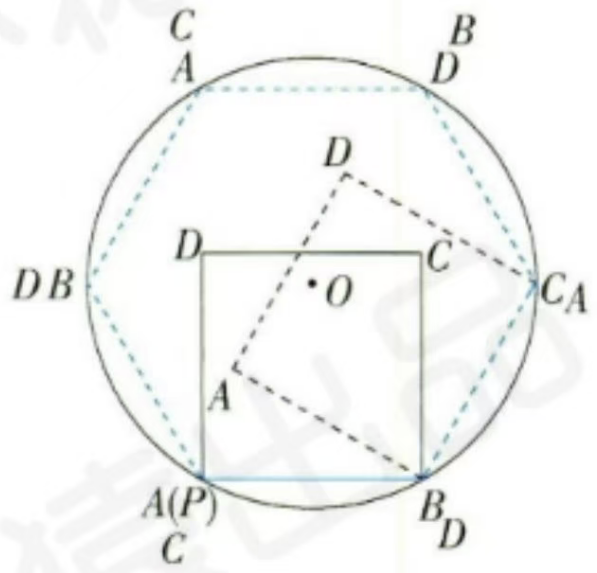
\includegraphics[width=0.2\linewidth]{bodyxb//src/image1.png}
        \end{center}
        正方形每次转动的角度为$\dfrac{\pi}{6}$，因此当点 $A$ 首次回到点 $P$ 的位置时,正方形滚动了 12 次,
        设第 $i$ 次滚动时,点 $A$ 走的路程为 ${A}_{i}$ ,
        则 ${A}_{1} = \dfrac{\pi }{6} \times  \left| {AB}\right|  = \dfrac{\pi }{3},{A}_{2} = \dfrac{\pi }{6} \times  \left| {AC}\right|  = \dfrac{\sqrt{2}\pi }{3}$ ,
        ${A}_{3} = \dfrac{\pi }{6} \times  \left| {DA}\right|  = \dfrac{\pi }{3},{A}_{4} = 0,$
        $\therefore$ 点 $A$ 所走过的路径的长度为 $3\left( {{A}_{1} + {A}_{2} + {A}_{3} + {A}_{4}}\right)  = (2 + \sqrt{2})\pi$ .
    \end{jieda} 
    \item 已知抛物线 ${y}^{2} = {ax}$ 与其关于点(2,1)对称的抛物线有 2 个不同的交点,且过这 2 个点的直线的倾斜角为 ${45}^{ \circ  }$ ,则实数 $a$ 的值是\blkda{2}.
    \begin{jieda}
        设点$(x_1, y_1)$在${y}^{2} = {ax}$上，点$(x_2, y_2)$在对称的抛物线上，两个点对称。因此有$\left\{\begin{array}{l}
             x_1 + x_2 = 4  \\
             y_1 + y_2 = 2
        \end{array}\right.$，代入抛物线方程得$(2-y_2)^2 = a(4-x_2)$，因此对称的抛物线方程为$(2-y)^2 = a(4-x)$
    
        联立两个抛物线方程$\left\{\begin{array}{l}
             (2-y)^2 = a(4-x)  \\
             {y}^{2} = {ax}
        \end{array}\right.$，消去$x$，可得$y^2-2y+(2+2a) = 0$，根据韦达定理有$\left\{\begin{array}{l}
             y_1+y_2 = 2 \\
             y_1y_2 = 2+2a
        \end{array}\right.$

        根据两点连线的倾斜角为$\ang{45}$可得$\dfrac{y_2-y_1}{x_2-x_1} = 1$，即$\dfrac{y_2-y_1}{a(y_2^2-y_1^2)} = 1$，即$y_1+y_2 = a$，因此$a = 2$
    \end{jieda}
    \item 如图,已知平面凸四边形 ${ABCD}$ 中, ${AB} = 1,{AD} = 2,\bigtriangleup {BCD}$ 是以 $D$ 为直角顶点的等腰直角三角形,那么 ${AC}$ 的最大值是\blkda{$1+2\sqrt{2}$}
    
    \begin{center}
    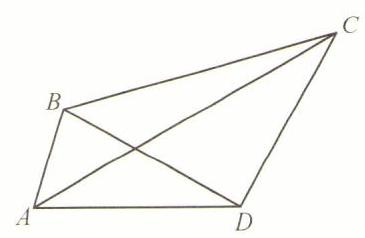
\includegraphics[width=0.3\textwidth]{bodyxb/src/bo_d1ig044601uc738hj6v0_86_1146_581_365_238_0.jpg}
    \end{center}
    \begin{jieda}
        \begin{enumerate}
            \item 方法1 

            过$D$做$DA' \perp DA$，且$|DA'| = |DA|$，且$A'$与$B$同侧，连接$A'C$，故$\triangle ADB$与$\triangle A'DC$全等，故$C$在以$A'$为圆心，1为半径的圆上，故$|AC|$的最大值为$1+2\sqrt{2}$
            \item 方法2

            设$\angle{BAD} = \theta$，则$|BD|^2 = 1+4-4cos\theta$，即$|BD| = \sqrt{5-4cos\theta}$，根据正弦定理有$\dfrac{sin\angle{ADB}}{1} = \dfrac{sin\theta}{\sqrt{5-4cos\theta}}$. 故$cos\angle{ADC} = -sin\angle{ADB} = -\dfrac{sin\theta}{\sqrt{5-4cos\theta}}$. 根据余弦定理有$|AC|^2 = 4 + |BD|^2 - 4|BD| \cdot cos\angle{ADC} = 4 + (5-4cos\theta) - 4\sqrt{5-4cos\theta} \times \left(-\dfrac{sin\theta}{\sqrt{5-4cos\theta}}\right) = 9-4cos\theta + 4sin\theta = 9 + 4\sqrt{2} sin\left(\theta - \dfrac{\pi}{4}\right)$，故$|AC| \leq 1+2\sqrt{2}$，当$\theta = \dfrac{3\pi}{4}$的时候取得最大值.
        \end{enumerate}
    \end{jieda}
    \item 已知双曲线 $C$ 的方程是 $\sqrt{{\left( x + 1\right) }^{2} + {\left( y - 1\right) }^{2}} - \left| {x - y - 2}\right|  = 0$ ,那么 $C$ 的焦距 $=$ \blkda{$8\sqrt{2}$}.
    \begin{jieda}
        $\sqrt{{\left( x + 1\right) }^{2} + {\left( y - 1\right) }^{2}} = \sqrt{2}\dfrac{\left| {x - y - 2}\right|}{\sqrt{2}}$
        
        根据双曲线定义,该方程描述的是以$(-1,1)$为焦点，直线 $x - y - 2 = 0$为准线，离心率为$\sqrt{2}$的双曲线。

        因此$\left\{\begin{array}{l}
             \dfrac{c}{a} = \sqrt{2} \\
             c - \dfrac{a^2}{c} = 2\sqrt{2}
        \end{array}\right.$解得$c = 4\sqrt{2}$，因此$2c = 8\sqrt{2}$
    \end{jieda}
\end{enumerate}

\subsection*{42 曲线的参数方程与 曲线系方程}

\subsubsection*{知识点睛}

1. 直线、圆、椭圆、双曲线、抛物线的参数方程都需要掌握,将参数方程消除参数,求出 $x$ , $y$ 的等式,即可得到一般方程. 我们也经常用三角代换去求出圆和椭圆的参数方程,继而用三角函数来进行计算.

2. 极坐标与直角坐标方程的转换满足 $\left\{  \begin{array}{l} x = \rho \cos \theta , \\  y = \rho \sin \theta , \end{array}\right.$ 对于一些非典型的极坐标方程,可以用这个方法逆转换成一般方程.

3. 曲线系常见的有两种情况,一种是过两个曲线交点的曲线,另一种是由点坐标满足一个二元方程, 得点在方程所对应曲线上. 若干个点均满足同一个等式, 则这些点均在该方程所对应的曲线上. 特别地,若两个点满足同一个二元一次方程,则该方程即为两点所确定的直线方程.

前者常见模型有:

(1) 经过 ${l}_{1} : {a}_{1}x + {b}_{1}y + {c}_{1} = 0$ 和 ${l}_{2} : {a}_{2}x + {b}_{2}y + {c}_{2} = 0$ 交点的直线为 ${a}_{1}x + {b}_{1}y + {c}_{1} +$  $\lambda \left( {{a}_{2}x + {b}_{2}y + {c}_{2}}\right)  = 0\left( {\text{ 不含 }{l}_{2}}\right) ;$

(2)经过 $l : {ax} + {by} + c = 0$ 和圆 ${x}^{2} + {y}^{2} + {Dx} + {Ey} + F = 0$ 交点(如果有)的圆为 ${x}^{2} +$  ${y}^{2} + {Dx} + {Ey} + F + \lambda \left( {{ax} + {by} + c}\right)  = 0;$

(3)经过圆 ${C}_{1} : {x}^{2} + {y}^{2} + {D}_{1}x + {E}_{1}y + {F}_{1} = 0$ 和圆 ${C}_{2} : {x}^{2} + {y}^{2} + {D}_{2}x + {E}_{2}y + {F}_{2} = 0$ 交点 (如果有) 的圆为 ${x}^{2} + {y}^{2} + {D}_{1}x + {E}_{1}y + F + \lambda \left( {{x}^{2} + {y}^{2} + {D}_{2}x + {E}_{2}y + {F}_{2}}\right)  = 0\left( {\lambda  \neq   - 1}\right)$ , 不含圆 ${C}_{2}$ ,特别地, $\lambda  =  - 1$ 时,该方程为圆的交点弦所在直线方程.

\subsubsection*{经典习题}

\begin{enumerate}
    \item 下列四组方程中表示不相同的曲线的是\dotfill{(\kh{C})}
    \xx{$\left\{  \begin{array}{l} x = 2\sin t, \\  y = 3\sin t \end{array}\right.$ 与 $y = \dfrac{3}{2}x,x \in  \left\lbrack  {-2,2}\right\rbrack$}{$\left\{  {\begin{array}{l} x = \tan \theta , \\  y = \cot \theta  \end{array}\left( {\theta  \neq  \dfrac{k\pi }{2},k \in  \mathbf{Z}}\right) }\right.$ 与 $y = \dfrac{1}{x}$}{$\left\{  \begin{array}{l} x = \dfrac{2t}{1 + {t}^{2}}, \\  y = \dfrac{1 - {t}^{2}}{1 + {t}^{2}} \end{array}\right.$ 与 ${x}^{2} + {y}^{2} = 1$}{$\left\{  \begin{array}{l} x = {t}^{2} - {3t} + 1, \\  y = t - 1 \end{array}\right.$ 与 $x = {y}^{2} - y - 1$}
    \begin{jieda}
        $t = 0, x = 0, y = 1$，而单位圆上有$(0, -1)$
    \end{jieda}
    \item 已知曲线 $\Gamma$ 的参数方程为 $\left\{  \begin{array}{l} x = {t}^{3} - t\cos t, \\  y = \ln \left( {t + \sqrt{{t}^{2} + 1}}\right) , \end{array}\right.$ 其中参数 $t \in  \mathbf{R}$ ,则曲线 $\Gamma$\dotfill{(\kh{C})}
    \xx{关于 $x$ 轴对称}{关于 $y$ 轴对称}{关于原点对称}{没有对称性}
    \begin{jieda}
        取一对互为相反数的$t_1, t_2$，则对应的$x_1+x_2 = 0, y_1+y_2 = 0$，因此曲线关于原点中心对称.
    \end{jieda}
    \item 若曲线 ${C}_{1} : \left\{  \begin{array}{l} x = 1 + \cos \theta , \\  y = \sin \theta  \end{array}\right.$ ( $\theta$ 为参数) 上的点 $P$ 到直线 ${C}_{2} : \left\{  \begin{array}{l} x = t \cdot  \sin {30}^{ \circ  }, \\  y = 1 - t \cdot  \cos {120}^{ \circ  } \end{array}\right.$ ( $t$ 为参数) 的距离最短,则点 $P$ 的坐标是\dotfill{(\kh{B})}
    \xx{$\left( {1 - \dfrac{\sqrt{2}}{2}, - \dfrac{\sqrt{2}}{2}}\right)$}{$\left( {1 - \dfrac{\sqrt{2}}{2},\dfrac{\sqrt{2}}{2}}\right)$}{$\left( {-\dfrac{\sqrt{2}}{2},1 - \dfrac{\sqrt{2}}{2}}\right)$}{$\left( {\dfrac{\sqrt{2}}{2},1 - \dfrac{\sqrt{2}}{2}}\right)$}
    \begin{jieda}
        $C_1: (x-1)^2+y^2 = 1$，$C_2: y = x+1$
    \end{jieda}
    \item 极坐标系下,若曲线 $\rho  = \dfrac{1}{1 - \sqrt{2}\cos \theta }$ 与曲线 ${\rho }^{2} - {2t\rho }\cos \theta  + {t}^{2} - 1 = 0$ 有公共点,则实数 $t$ 的取值范围是\blkda[3]{$[-\sqrt{2}-2, 2-\sqrt{2}]$}.
    \begin{jieda}
        $\rho  = \dfrac{1}{1 - \sqrt{2}\cos \theta }$即$(x+\sqrt{2})^2 - y^2 = 1$
        
        ${\rho }^{2} - {2t\rho }\cos \theta  + {t}^{2} - 1 = 0$即$(x-t)^2+y^2 = 1$

        曲线在极坐标下有交点，即在直角坐标下有交点，联立两式消去$y$可得$2x^2+(2\sqrt{2}-2t)x+t^2=0$，$\Delta = (2\sqrt{2}-2t)^2-8t^2 \geq 0$，解得$t \in [-\sqrt{2}-2, 2-\sqrt{2}]$
    \end{jieda}
    \item 在平面直角坐标系 ${xOy}$ 中,已知椭圆 ${C}_{1} : \dfrac{{x}^{2}}{36} + \dfrac{{y}^{2}}{4} = 1$ 和 ${C}_{2} : {x}^{2} + \dfrac{{y}^{2}}{9} = 1.P$ 为 ${C}_{1}$ 上的动点, $Q$ 为 ${C}_{2}$ 上的动点, $w$ 是 $\vv{OP} \cdot  \vv{OQ}$ 的最大值. 记 $\Omega  = \left\{  {\left( {P,Q}\right)  \mid  P}\right.$ 在 ${C}_{1}$ 上, $Q$ 在 ${C}_{2}$ 上,且 $\vv{OP}$ . $\vv{OQ} = w\}$ ,则 $\Omega$ 中元素个数为 \dotfill{(\kh{D})}
    \xx{2 个}{4 个}{8 个}{无穷个}
    \begin{jieda}
        $C_1: \left\{\begin{array}{l}
             x = 6cos\theta  \\
             y = 2sin\theta
        \end{array} \right.$，故$P(6cos\alpha, 2sin\alpha)$，$C_2 : \left\{\begin{array}{l}
             x = cos\theta \\
             y = 3sin\theta
        \end{array}\right.$，故$Q(cos\beta, 3sin\beta)$，因此$\vv{OP} \cdot  \vv{OQ} = 6cos\alpha \cdot cos\beta + 6sin\alpha \cdot sin\theta = 6cos(\alpha - \beta)$，当$\alpha = \beta$时$\vv{OP} \cdot  \vv{OQ}$取得最大值.
    \end{jieda}
    \item 设抛物线 $\left\{  \begin{array}{l} x = {2p}{t}^{2}, \\  y = {2pt} \end{array}\right.$ ( $t$ 为参数, $p > 0$ ) 的焦点为 $F$ ,准线为 $l$ . 过抛物线上一点 $A$ 作 $l$ 的垂线,垂足为 $B$ . 设 $C\left( {\dfrac{7}{2}p,0}\right) ,{AF}$ 与 ${BC}$ 相交于点 $E$ . 若 $\left| {CF}\right|  = 2\left| {AF}\right|$ ,且 $\bigtriangleup {ACE}$ 的面积为 $3\sqrt{2}$ ,则 $p$ 的值为\blkda{$\sqrt{6}$}.
    \begin{jieda}
        抛物线方程为$y^2 = 2px$，$|CF| = 3p$，故$|AF| = \dfrac{3p}{2}$，因此$|AB| = \dfrac{3p}{2}$，根据抛物线的定义可知$x_A = p$，故$A(p. \sqrt{2}p)$

        $AF: y = 2\sqrt{2}\left(x-\dfrac{p}{2}\right)$，$BC: y = -\dfrac{\sqrt{2}}{4}\left(x-\dfrac{7p}{2}\right)$

        联立解得$E\left(\dfrac{5p}{6}, \dfrac{2\sqrt{2}p}{3}\right)$，故$\vv{EA} = \left(\dfrac{p}{6}, \dfrac{\sqrt{2}p}{3}\right)$，$\vv{EC} = \left(\dfrac{8p}{3}, -\dfrac{2\sqrt{2}p}{3}\right)$，故$S_{\triangle ACE} = \dfrac{1}{2}\left|\dfrac{p}{6} \times \left(-\dfrac{2\sqrt{2}p}{3} + \dfrac{\sqrt{2}p}{3} \times \dfrac{8p}{3}\right)\right| = 3\sqrt{2}$，解得$p = \sqrt{6}$
    \end{jieda}
    \item 平面直角坐标系 ${xOy}$ 中,三角形 ${ABC}$ 的顶点坐标分别为 $A\left( {0,a}\right) ,B\left( {b,0}\right) ,C\left( {c,0}\right)$ ,点 $P\left( {0,p}\right)$ 在线段 ${OA}$ 上 (异于端点),设 $a,b,c,p$ 均为非零实数,直线 ${BP},{CP}$ 分别交 ${AC},{AB}$ 于点 $E,F$ ,一同学已正确算出 ${OE}$ 的方程: $\left( {\dfrac{1}{b} - \dfrac{1}{c}}\right) x + \left( {\dfrac{1}{p} - \dfrac{1}{a}}\right) y = 0$ ,则直线 ${OF}$ 的方程为\blkda[5]{$\left( {\dfrac{1}{c} - \dfrac{1}{b}}\right) x + \left( {\dfrac{1}{p} - \dfrac{1}{a}}\right) y = 0$}.
    \begin{jieda}
        由对称性可猜想 $\left( {\dfrac{1}{c} - \dfrac{1}{b}}\right) x + \left( {\dfrac{1}{p} - \dfrac{1}{a}}\right) y = 0$ .
        事实上,由截距式可得直线 ${AB} : \dfrac{x}{a} + \dfrac{y}{b} = 1$ ,直线 ${CP} : \dfrac{x}{c} + \dfrac{y}{p} = 1$ ,两式相减得 $\left( {\dfrac{1}{c} - \dfrac{1}{b}}\right) x + \left( {\dfrac{1}{p} - \dfrac{1}{a}}\right) y = 0$ ,显然直线 ${AB}$ 与 ${CP}$ 的交点 $F$ 满足此
        方程,又原点 $O$ 也满足此方程,故为所求的直线 ${OF}$ 的方程.
    \end{jieda}
    \item 已知抛物线 ${\Gamma }_{1}$ 与 ${\Gamma }_{2}$ 的焦点均为点 $F\left( {2,1}\right)$ ,准线方程分别为 $x = 0$ 与 ${5x} + {12y} = 0$ . 设两抛物线交于 $A$ 、 $B$ 两点,则直线 ${AB}$ 的方程为\blkda{$y = \dfrac{2}{3}x$}.
    \begin{jieda}
        按抛物线定义有 ${\Gamma }_{1} : {\left( x - 2\right) }^{2} + {\left( y - 1\right) }^{2} = {x}^{2};{\Gamma }_{2} : {\left( x - 2\right) }^{2} + {\left( y - 1\right) }^{2} = \dfrac{{\left( 5x + {12}y\right) }^{2}}{{13}^{2}}$ 
        
        两方程相减即得 ${x^2} = \dfrac{{\left( 5x + {12}y\right) }^{2}}{{13}^{2}}$ ,而结合图像可知 $A,B$ 位于 $x = 0$ 的右侧和 ${5x} + {12y} = 0$ 的上侧,
        故 $x = \dfrac{{5x} + {12y}}{13}$ ,即 $y = \dfrac{2}{3}x$ .
        故答案为: $y = \dfrac{2}{3}x$ .
    \end{jieda}
    \item 已知函数 $y = {x}^{2} + {ax} + b$ 过定点$(-1,3)$,且与坐标轴有 3 个不同的交点 $A,B,C$ ,那么经过 $A,B,C$ 三点的圆一定经过定点\blkda[3]{$(0, 1)$和$\left(\dfrac{1}{2}, \dfrac{3}{2}\right)$}.
    \begin{jieda}
        设圆的方程为$x^2+y^2+Dx+Ey+F = 0$
        \begin{dingautolist}{172}
            \item 当$x = 0$时，$y^2+Ey+F=0$，$y = b$是一个根，因此$b^2+Eb+F=0$
            \item 当$y = 0$时，$x^2+Dx+F=0$与${x}^{2} + {ax} + b = 0$的根相同，因此$D = a, F = b$
        \end{dingautolist}
        综上，圆的方程为$x^2+y^2+ax-(b+1)y+b = 0$

        因为$y = {x}^{2} + {ax} + b$ 过定点$(-1,3)$，所以$b = a+2$，因此圆的方程可以进一步化简为$x^2+y^2+ax-(a+3)y+a+2 = 0$，整理成关于$a$的等式，即$(x-y+1)a+(x^2+y^2-3y+2) = 0$，要使得圆过定点，应有$\left\{\begin{array}{l}
             x-y+1 = 0  \\
             x^2+y^2-3y+2 = 0 
        \end{array} \right.$，解得$x = 0, y = 1$或$x = \dfrac{1}{2}, y = \dfrac{3}{2}$，因此圆过的定点为$(0, 1)$和$\left(\dfrac{1}{2}, \dfrac{3}{2}\right)$
    \end{jieda}
\end{enumerate}

\subsection*{43 新定义问题}

\subsubsection*{知识点睛}

解决此类问题比较常见的思路是通过分类讨论画出图象,再利用图象判断各种性质. 要注意的是,曲线方程 $f\left( {x,y}\right)  = 0$ 中,如果 $f\left( {-x,y}\right)  = f\left( {x,y}\right)$ 恒成立,则曲线关于 $y$ 轴对称; 如果 $f\left( {x, - y}\right)  = f\left( {x,y}\right)$ 恒成立,则曲线关于 $x$ 轴对称；如果 $f\left( {-x, - y}\right)  = f\left( {x,y}\right)$ 恒成立,那么曲线关于原点对称. 如果 $f\left( {y,x}\right)  = f\left( {x,y}\right)$ 恒成立,那么曲线关于 $y = x$ 轴对称.

\subsubsection*{经典习题}
\begin{enumerate}
    \item 在平面直角坐标系 ${xOy}$ 中, $O$ 为坐标原点. 定义 $P\left( {{x}_{1},{y}_{1}}\right) \text{ 、 }Q\left( {{x}_{2},{y}_{2}}\right)$ 两点之间的曼哈顿距离为 $d\left( {P,Q}\right)  = \left| {{x}_{1} - {x}_{2}}\right|  + \left| {{y}_{1} - {y}_{2}}\right|$ . 已知 $B\left( {1,1}\right)$ ,点 $M$ 为直线 $x - y + 4 = 0$ 上的动点,则 $d\left( {B,M}\right)$ 的最小值为\blkda{4}.
    \begin{jieda}
        设$M(m, m+4)$，则$BD$的曼哈顿距离$|m-1|+|m+4-1| = |m-1|+|m+3| \geq 4$
    \end{jieda}
    \item 若 $x,y \in  \mathbf{R},M = \{ \left( {x,y}\right) \mid \left| x \right| + \left| y \right| < 1\} ,N = \{ \left( {x,y}\right) \mid \left| x + y \right|< 1, \left| x \right| < 1$ , $\left| y\right|  < 1\} ,P = \left\{  {\left( {x,y}\right)  \mid  \sqrt{{\left( x - {0.5}\right) }^{2} + {\left( y + {0.5}\right) }^{2}} + \sqrt{{\left( x + {0.5}\right) }^{2} + {\left( y - {0.5}\right) }^{2}} < }\right.$  $2\sqrt{2}\}$ ,则\dotfill{(\kh{A})}
    \xx{$M \subset  N \subset  P$}{$N \subset  M \subset  P$}{$M \subset  P \subset  N$}{以上皆错}
    \begin{jieda}
        \begin{center}
            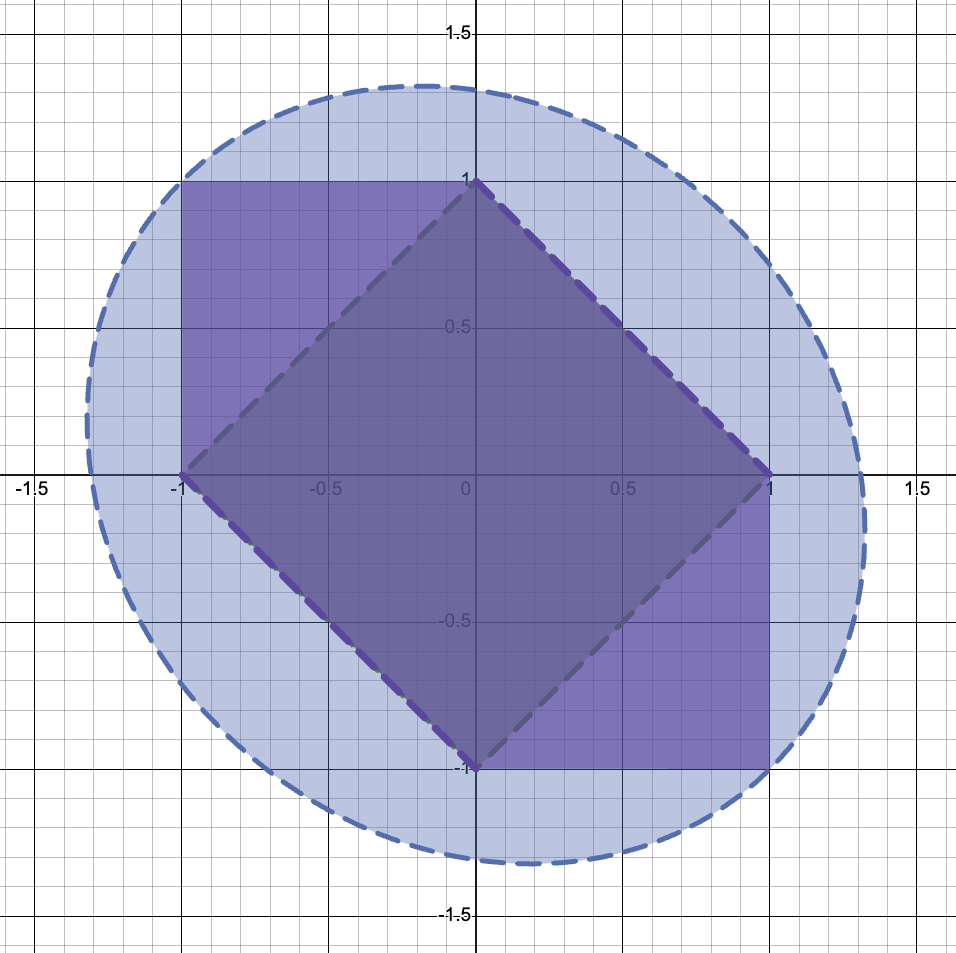
\includegraphics[width=0.3\linewidth]{bodyxb//src/43-1.png}
        \end{center}
    \end{jieda}
    \item 已知平面区域 ${C}_{1} : {x}^{2} + {y}^{2} \leq  4\left( {\left| x\right|  + \left| y\right| }\right)$ ,则平面区域 ${C}_{1}$ 的面积为\blkda{$32+16\pi$}.
    \begin{jieda}
        根据$C_1$的形式可知其区域关于$x$轴和$y$轴均对称，因此只需要考虑第一象限内的图形

        在第一象限内，直接去掉绝对值有${x}^{2} + {y}^{2} \leq  4\left( x+y\right)$，即$(x-2)^2+(y-2)^2 \leq 8$，故为一直角三角形和一半圆拼接而成，第一象限内的面积为$S_1 = \dfrac{1}{2} \times 4 \times 4 + \dfrac{1}{2} \times \pi \times 8 = 8 + 4\pi$，故$C_1$的面积$S = 32+16\pi$

        $C_1$示意图如下：
        \begin{center}
            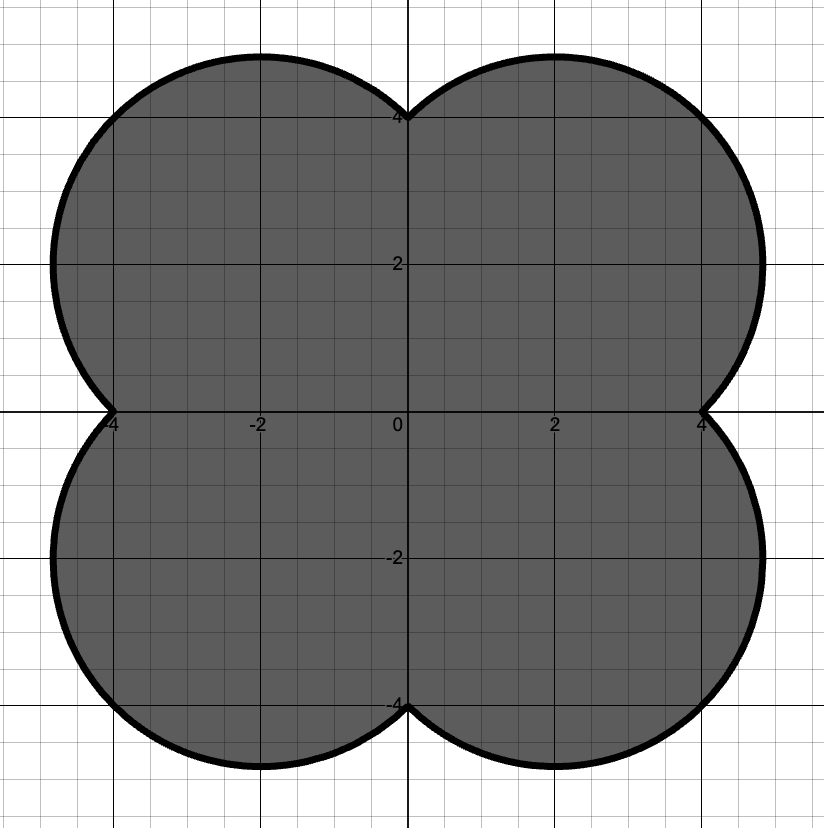
\includegraphics[width=0.3\linewidth]{bodyxb//src/43-2.png}
        \end{center}
    \end{jieda}
    \item 已知实数 $x\text{ 、 }y$ 满足 $\dfrac{x\left| x\right| }{4} - y\left| y\right|  = 1$ ,则 $\left| {x - {2y}}+\sqrt{5}\right|$ 的取值范围是\blkda[3]{$(\sqrt{5}, 2\sqrt{2}+\sqrt{5}]$}.
    \begin{jieda}
        分类讨论可知该方程即$\left\{\begin{array}{ll}
             \dfrac{x^2}{4}-y^2 = 1, & (x, y)\text{在第一象限}  \\
             -\dfrac{x^2}{4}+y^2 = 1, & (x, y)\text{在第三象限}  \\
             \dfrac{x^2}{4}+y^2 = 1, & (x, y)\text{在第四象限}
        \end{array}\right.$，为一段连续的曲线.

        易知曲线上的点到直线$x-2y+\sqrt{5} = 0$的距离为$\dfrac{\left| {x - {2y}}+\sqrt{5}\right|}{\sqrt{5}}$，结合图像可知：
        \begin{dingautolist}{172}
            \item 曲线在一三象限的两段双曲线，其渐近线为$x - 2y = 0$，可以取到目标值的下界：$\left| {x - {2y}}+\sqrt{5}\right| > \sqrt{5}$
            \item 曲线在第四象限的椭圆，当切线与直线$x-2y+\sqrt{5} = 0$平行时，切点处取得目标值的最大值，设切点为$(a, b)$，则切线为$\dfrac{ax}{4}+by = 1$，故当$b = -\dfrac{a}{2}$时，切线满足要求，故切点为$\left(a, -\dfrac{a}{2}\right)$，代入曲线方程有$a = \sqrt{2}$，故切点为$\left(\sqrt{2}, -\dfrac{\sqrt{2}}{2}\right)$，故$\left| {x - {2y}}+\sqrt{5}\right| \leq 2\sqrt{2}+\sqrt{5}$
        \end{dingautolist}
        综上，$\left| {x - {2y}}+\sqrt{5}\right| \in (\sqrt{5}, 2\sqrt{2}+\sqrt{5}]$
    \end{jieda}
    \item 方程 $\dfrac{x\left| x\right| }{16} + \dfrac{y\left| y\right| }{9} =  - 1$ 的曲线即为函数 $y = f\left( x\right)$ 的图象,对于函数 $y = f\left( x\right)$ ,有如下结论:\ding{172} $f\left( x\right)$ 在 $\mathbf{R}$ 上单调递减；\ding{173}函数 $F\left( x\right)  = {4f}\left( x\right)  + {3x}$ 不存在零点；\ding{174}函数 $y = f\left( x\right)$ 的值域是 $\mathbf{R}$ ；\ding{175}若函数 $g\left( x\right)$ 和 $f\left( x\right)$ 的图象关于原点对称,则 $y = g\left( x\right)$ 由方程 $\dfrac{y\left| y\right| }{16} + \dfrac{x\left| x\right| }{9} = 1$ 确定. 其中所有正确的命题序号是\dotfill{(\kh{D})}
    \xx{\ding{172}\ding{174}}{\ding{172}\ding{175}}{\ding{172}\ding{174}\ding{175}}{\ding{172}\ding{173}\ding{174}}
    
    \begin{jieda}
        分类讨论可知该方程即$\left\{\begin{array}{ll}
             \dfrac{x^2}{16}-\dfrac{y^2}{9} = 1, & (x, y)\text{在第二象限}  \\
             \dfrac{x^2}{16}+\dfrac{y^2}{9} = 1, & (x, y)\text{在第三象限}  \\
             -\dfrac{x^2}{16}+\dfrac{y^2}{9} = 1, & (x, y)\text{在第四象限}
        \end{array}\right.$，为一段连续的曲线
        \begin{dingautolist}{172}
            \item 结合图像易知$f(x)$单调递减
            \item $f(x)$在二四象限的两段双曲线的渐近线为$y = -\dfrac{3}{4}x$，$F\left( x\right)  = {4f}\left( x\right)  + {3x}$ 不存在零点即$y = f(x) + \dfrac{3}{4}x$没有零点，即$y = f(x)$与$y = -\dfrac{3}{4}x$没有交点，结合图像可知正确
            \item 结合图像易知函数 $y = f\left( x\right)$ 的值域是 $\mathbf{R}$
            \item $y = g\left( x\right)$ 应由方程 $\dfrac{y\left| y\right| }{9} + \dfrac{x\left| x\right| }{16} = 1$ 确定，故错误
        \end{dingautolist}
    \end{jieda}
    
    \item 在平面直角坐标系中, $O$ 为坐标原点,设点 $P\left( {x,y}\right)$ ,定义 $\left\lbrack  {OP}\right\rbrack   = \left| x\right|  + \left| y\right|$ ,对于下列两个命题:
    \begin{dingautolist}{172}
        \item 设点 $P$ 是直线 $y = {kx} + 1\left( {k \in  {R}}\right)$ 上任意一点,则 “使得 $\left\lbrack  {OP}\right\rbrack$ 最小的点 $P$ 有无数个” 的充要条件是“ $k =  \pm  1$ ”
        \item 设点 $P$ 是椭圆 $\dfrac{{x}^{2}}{4} + {y}^{2} = 1$ 上任意一点,则 ${\left\lbrack  OP\right\rbrack  }_{max } = \sqrt{5}$
    \end{dingautolist}
    则下列判断正确的是\dotfill{(\kh{A})}
    \xx{\ding{172}真\ding{173}真}{\ding{172}真\ding{173}假}{\ding{172}假\ding{173}真}{\ding{172}假\ding{173}假}
    \begin{jieda}
        对于$c \in \mathbf{R}$，$[OP] = c$所对应的图形是一个以原点为中心，坐标轴为对角线的的正方形，若直线$y = {kx} + 1\left( {k \in  {R}}\right)$的斜率$k \neq \pm 1$，则其必然与$[OP] = c$只有有限个公共点，故使得 $\left\lbrack  {OP}\right\rbrack$ 最小的点 $P$ 只有有限个，而当$k = \pm 1$时，则有无限个.

        当椭圆$\dfrac{{x}^{2}}{4} + {y}^{2} = 1$的切线斜率为$\pm 1$的时候，取得$[OP]_{max}$，考虑第一象限内的切点，为$(a, b), a > 0, b > 0$，则$\dfrac{ax}{4}+by = 1$，故$b = \dfrac{a}{4}$，即切点为$\left(a, \dfrac{a}{4}\right)$，代入椭圆方程有$a = \dfrac{4\sqrt{5}}{5}, b = \dfrac{\sqrt{5}}{5}$，故$[OP]_{max} = \sqrt{5}$
        \end{jieda}

    \item 在平面直角坐标系中,当 $P\left( {x,y}\right)$ 不是原点时,定义 $P$ 的 “伴随点” 为 ${P}^{\prime }\left( {\dfrac{y}{{x}^{2} + {y}^{2}}\text{ , }}\right.$  $\left. \dfrac{-x}{{x}^{2} + {y}^{2}}\right)$ ,当 $P$ 是原点时,定义“伴随点”为它自身,现有下列命题:
    \begin{dingautolist}{172}
        \item 若点 $A$ 的 “伴随点” 是点 ${A}^{\prime }$ ,则点 ${A}^{\prime }$ 的 “伴随点” 是点 $A$
        \item 单位圆上的“伴随点”还在单位圆上
        \item 若两点关于 $x$ 轴对称,则它们的“伴随点”关于 $y$ 轴对称
        \item 若三点在同一条直线上,则它们的“伴随点”一定共线
    \end{dingautolist}
    其中真命题是\blkda{\ding{173}\ding{174}}(编号按从小到大顺序填写).
    \begin{jieda}
        \begin{dingautolist}{172}
            \item 代特值$P(2, 0)$得到$P'(0, -2)$，得到$P''(-2, 0)$，故错误
            \item 设$P(cos\alpha, sin\alpha)$，则$P'(sin\alpha, -cos\alpha)$，对于任意$\alpha$恒成立，故正确
            \item 根据对称性定义显然正确
            \item 代入特值$A(-1, 0), B(0, 1), C(1, 2)$可得$A'(0, 1), B'(1, 0), C'\left(\dfrac{2}{5}, -\dfrac{1}{5}\right)$，故错误
        \end{dingautolist}
    \end{jieda}
    \item 方程 $2{x}^{2} - {9xy} + 8{y}^{2} = 0$ 的曲线 $C$ 所满足的性质为\dotfill{(\kh{A})}
    \begin{dingautolist}{172}
        \item 不经过第二、四象限
        \item 关于 $x$ 轴对称
        \item 关于原点对称
        \item 关于直线 $y = x$ 对称
    \end{dingautolist}
    \xx{\ding{172}\ding{174}}{\ding{173}\ding{174}}{\ding{172}\ding{175}}{\ding{172}\ding{173}}
    \begin{jieda}
        \begin{dingautolist}{172}
            \item 若在二四象限，则$xy < 0$，则等式左侧必然为正，不可能成立，故正确
            \item $y$取互为相反数的值，等式左侧值变化，故错误
            \item $x, y$均取相反数，等式左侧值不变，故正确
            \item $x, y$的值互换，等式左侧值变化，故错误
        \end{dingautolist}
    \end{jieda}
    \item 已知曲线 $C : \dfrac{x\left| x\right| }{{a}^{2}} - \dfrac{y\left| y\right| }{{b}^{2}} = 1$ ,下列叙述中错误的是\dotfill{(\kh{C})}
    \xx{垂直于 $x$ 轴的直线与曲线 $C$ 只有一个交点}{直线 $y = {kx} + m\left( {k,m \in  \mathbf{R}}\right)$ 与曲线 $C$ 最多有三个交点}{曲线 $C$ 关于直线 $y =  - x$ 对称}{若 ${P}_{1}\left( {{x}_{1},{y}_{1}}\right) \text{ 、 }{P}_{2}\left( {{x}_{2},{y}_{2}}\right)$ 为曲线 $C$ 上任意两点,则有 $\dfrac{{y}_{1} - {y}_{2}}{{x}_{1} - {x}_{2}} > 0$}
    \begin{jieda}
        数形结合可知
    \end{jieda}
    \item 曲线 $C$ 是平面内与两个定点 ${F}_{1}\left( {-1,0}\right)$ 和 ${F}_{2}\left( {1,0}\right)$ 的距离的积等于常数 ${a}^{2}\left( {a > 1}\right)$ 的点的轨迹. 给出下列三个结论:
    \begin{dingautolist}{172}
        \item 曲线 $C$ 过坐标原点
        \item 曲线 $C$ 关于坐标原点对称
        \item 若点 $P$ 在曲线 $C$ 上,则 $\bigtriangleup {F}_{1}P{F}_{2}$ 的面积不大于 $\dfrac{1}{2}{a}^{2}$
    \end{dingautolist}
    其中正确命题的序号为\blkda{\ding{173}\ding{174}}.
    \begin{jieda}
        \begin{enumerate}
            \item 代入原点可知，其到两定点之积为1，与$a > 1$矛盾
            \item 若$(x_0, y_0)$在曲线上，则$(-x_0, -y_0), (x_0, -y_0), (-x_0, y_0)$均在曲线上
            \item 设$|PF_1| = m, |PF_2| = n$，$mn = a^2$，$S = \dfrac{1}{2}mnsin\theta < \dfrac{1}{2}mn = \dfrac{1}{2}a^2$，故正确
        \end{enumerate}
    \end{jieda}
\end{enumerate}


\subsection*{44 曲线中的定点定值 与向量问题}

\subsubsection*{知识点睛}

定点定值问题需要掌握圆锥曲线中的一些二级结论,包括但不限于第一定义可得焦半径之和或者差是定值；第二定义可得 $\dfrac{\mid {PF} \mid  }{d} = e$ 为定值；第三定义可得,已知圆锥曲线上两个关于对称中心对称的点 $A$ 、 $B$ ,则同一曲线上任意其他点 $P$ ,有 ${PA}$ 、 ${PB}$ 的斜率(若存在)乘积为定值. 更复杂的定点定值问题一般出现在解答题中, 需要用韦达定理等方法处理.

另外如果选择和填空题涉及定点定值问题时,可以直接用特殊法进行赋值计算答案,避开复杂的解题过程.

圆锥曲线中的向量问题基本上都是用坐标运算, 直接设动点坐标计算即可, 有时会用向量的几何意义去进行解答.

\subsubsection*{经典习题}
\begin{enumerate}
    \item 若双曲线 ${x}^{2} - {y}^{2} = {a}^{2}\left( {a > 0}\right)$ 的左、右顶点分别为 $A\text{ 、 }B$ ,点 $P$ 是第一象限内双曲线上的点. 若直线 ${PA}\text{ 、 }{PB}$ 的倾斜角分别为 $\alpha ,\beta$ ,且 $\beta  = {m\alpha }\left( {m > 1}\right)$ ,那么 $\alpha$ 的值是\dotfill{(\kh{D})}
    \xx{$\dfrac{\pi }{{2m} - 1}$}{$\dfrac{\pi }{2m}$}{$\dfrac{\pi }{{2m} + 1}$}{$\dfrac{\pi }{{2m} + 2}$}
    \begin{jieda}
        根据双曲线的第三定义可知$tan\alpha \cdot tan\beta = e^2 - 1 = (\sqrt{2})^2 - 1 = 1$，故$\alpha + \beta = \dfrac{\pi}{2}$，即$(m+1)\alpha = \dfrac{\pi}{2}$，因此$\alpha = \dfrac{\pi}{2(m+1)}$
    \end{jieda}
    \item 已知双曲线 $\dfrac{{x}^{2}}{{a}^{2}} - \dfrac{{y}^{2}}{2{a}^{2}} = 1$ 的左、右顶点分别为 ${A}_{1}\text{ 、 }{A}_{2},P$ 为双曲线右支上一点,且位于第一象限,直线 $P{A}_{1}\text{ 、 }P{A}_{2}$ 的斜率分别为 ${k}_{1}\text{ 、 }{k}_{2}$ ,则 $\dfrac{1}{{k}_{1}} + \dfrac{1}{{k}_{2}}$ 的取值范围是\blkda{$(\sqrt{2}, +\infty)$}.
    \begin{jieda}
        根据双曲线的第三定义可知$k_1 \cdot k_2 = e^2 - 1 = 3 - 1 = 2$，所以$\dfrac{1}{k_1} + \dfrac{1}{k_2} = k_1 + \dfrac{1}{k_1}$

        因为$P$ 为双曲线右支上一点,且位于第一象限，所以$k_1 \in (1, +\infty)$，因此$k_1 + \dfrac{1}{k_1} \in (\sqrt{2}, +\infty)$
    \end{jieda}

    \item 双曲线 ${x}^{2} - \dfrac{{y}^{2}}{3} = 1$ 的左、右两支上各有一点 $A\text{ 、 }B$ ,点 $B$ 在直线 $x = \dfrac{1}{2}$ 上的射影是点 ${B}^{\prime }$ ,若直线 ${AB}$ 过右焦点,则直线 $A{B}^{\prime }$ 必定经过的定点坐标为\blkda{$\left(\dfrac{5}{4}, 0\right)$}.
    \begin{jieda}
        设$A(x_1, y_1), B(x_2, y_2)， B'\left(\dfrac{1}{2}, y_2\right)$，右焦点$F(2, 0)$

        设$AB: y = k(x-2), k = \dfrac{y_2 - y_1}{x_2 - x_1}$，设$AB': y - y_1 = k'(x - x_1), k' = \dfrac{y_2-y_1}{\dfrac{1}{2} - x_1} = \dfrac{x_2-x_1}{\dfrac{1}{2} - x}k$，故$AB'$可以表示为$y - k(x_1-2) = \dfrac{x_2-x_1}{\dfrac{1}{2} - x_1}k(x-x_1)$

        易知$x_1 \neq \dfrac{1}{2}$，故欲证$AB'$过定点，可以先去分母，即证$\left(\dfrac{1}{2} - x_1\right)y + k(x_1-2)\left(x_1 - \dfrac{1}{2}\right) = (x_2 - x_1)kx -x_1x_2k + kx_1^2$

        易知该方程对于$x_1, x_2$应是轮换对称的，故可以将其整理成$x_1, x_2$为主元的式子，即$\left(-y - \dfrac{5}{2}k+kx\right)x_1  - (kx)x_2 + \left(\dfrac{1}{2}y+k+x_1x_2k\right) = 0$. 最后一项对于$x_1, x_2$是轮换对称的，因此必有前两项的系数相等，即$y + \dfrac{5}{2} - kx = kx$

        若$AB'$过定点$(x_0, y_0)$，则对任意的$x_1, x_2$，等式代入$(x_0, y_0)$均成立，则应有$y_0 + \dfrac{5}{2} - kx_0 = kx_0$恒成立，而$k$并非定值，因此$x_0 = \dfrac{5}{4}, y_0 = 0$可以使得等式恒成立，故若存在满足题干要求的顶点，则必为$\left(\dfrac{5}{4}, 0\right)$

        下证$A{B}^{\prime }$ 必定经过的定点$\left(\dfrac{5}{4}, 0\right)$：

        将$\left(\dfrac{5}{4}, 0\right)$代入$\left(-y - \dfrac{5}{2}k+kx\right)x_1  - (kx)x_2 + \left(\dfrac{1}{2}y+k+x_1x_2k\right) = 0$，可得$LHS = -\dfrac{5}{4}k(x_1+x_2)+k+x_1x_2 = k\left(1+x_1x_2-\dfrac{5}{4}(x_1+x_2)\right)$
        
        联立$\left\{\begin{array}{l}
             y = k(x-2) \\
             x^2 - \dfrac{y^2}{3} = 1
        \end{array}\right.$，消去$y$可得$3x^2-k^2(x-2)^2 = 3$，整理得$(3-k^2)x^2+4k^2x-(4k^2+3) = 0$，根据韦达定理有$\left\{\begin{array}{l}
             x_1+x_2 = \dfrac{4k^2}{k^2-3} \\
             x_1x_2 = \dfrac{4k^2+3}{k^2-3}
        \end{array}\right.$，代入可得$LHS = k\left(1+x_1x_2-\dfrac{5}{4}(x_1+x_2)\right) = 0 = RHS$
    \end{jieda}
    \item 已知直线 ${l}_{1} : {mx} - y = 0,{l}_{2} : x + {my} - m - 2 = 0,{l}_{1}$ 与 ${l}_{2}$ 的交点为 $P,O$ 为原点,当 $m$ 在实数范围内变化时, $\left| {PO}\right|$ 的取值范围是\blkda{$[0, \sqrt{5}]$}.
    \begin{jieda}
        观察可知$l_1 \perp l_2$，$l_1$恒过$O(0, 0)$，$l_2$恒过$A(2, 1)$，故$P$的轨迹应为以$OA$为直径的圆，因此$|PO| \in [0, \sqrt{5}]$
    \end{jieda}
    \item 已知椭圆 $C : \dfrac{{x}^{2}}{2} + \dfrac{{y}^{2}}{4} = 1$ 的上、下焦点分别为 ${F}_{1}\text{ 、 }{F}_{2}$ ,过椭圆 $C$ 上一点 $P\left( {1,\sqrt{2}}\right)$ 作倾斜角互补的两条直线 ${PA}$ 、 ${PB}$ ,分别交椭圆 $C$ 于 $A$ 、 $B$ 两点,则直线 ${AB}$ 的斜率为\blkda{$\sqrt{2}$}.
    \begin{jieda}
        取特值：
        
        $A$与$P$关于原点中心对称，则$k_{PA} = \sqrt{2}$，故$k_{PB} = -\sqrt{2}$，根据椭圆的第三定义可知$k_{AB} \cdot k_{PB} = \dfrac{1}{e^2 - 1} = -2$，故$k_{AB} = \sqrt{2}$

        正常求解：
        
        根据题意设 $A\left( {{x}_{1},{y}_{1}}\right) ,B\left( {{x}_{2},{y}_{2}}\right)$
        
        直线 ${PA}$ 的直线方程为 $y - \sqrt{2} = k\left( {x - 1}\right)$ ,代入方程 $\dfrac{{x}^{2}}{2} + \dfrac{{y}^{2}}{4} = 1$，消去$y$整理得$\left( {{k}^{2} + 2}\right) {x}^{2} - {2k}\left( {k - \sqrt{2}}\right) x + {k}^{2} - 2\sqrt{2}k - 2 = 0$，根据韦达定理有 ${x}_{1} \times  1 = \dfrac{{k}^{2} - 2\sqrt{2}k - 2}{{k}^{2} + 2}$，故 ${x}_{1} = \dfrac{{k}^{2} - 2\sqrt{2}k - 2}{{k}^{2} + 2},{y}_{1} = \dfrac{-\sqrt{2}{k}^{2} - {4k} + 2\sqrt{2}}{{k}^{2} + 2}$
        
        因为直线 ${PA}$ 、 ${PB}$ 的倾斜角互补，所以用 $- k$ 代替 ${x}_{1},{y}_{1}$ 中的 $k$，得 ${x}_{2} = \dfrac{{k}^{2} + 2\sqrt{2}k - 2}{{k}^{2} + 2},{y}_{2} = \dfrac{-\sqrt{2}{k}^{2} + {4k} + 2\sqrt{2}}{{k}^{2} + 2}$
        
        所以 ${k}_{AB} = \dfrac{{y}_{2} - {y}_{1}}{{x}_{2} - {x}_{1}} = \sqrt{2}$ 
    \end{jieda}

    \item 已知圆 $M : {x}^{2} + {\left( y - 1\right) }^{2} = 1$ ,圆 $N : {x}^{2} + {\left( y + 1\right) }^{2} = 1$ ,直线 ${l}_{1}\text{ 、 }{l}_{2}$ 分别过圆心 $M\text{ 、 }N$ ,且 ${l}_{1}$ 与圆 $M$ 相交于 $A$ 、 $B$ 两点, ${l}_{2}$ 与圆 $N$ 相交于 $C\text{ 、 }D$ 两点,点 $P$ 是椭圆 $\dfrac{{x}^{2}}{9} + \dfrac{{y}^{2}}{4} = 1$ 上任意一点,则 $\vv{PA} \cdot  \vv{PB} + \vv{PC} \cdot  \vv{PD}$ 的最小值为\blkda{8}.
    \begin{jieda}
        根据极化恒等式可知$\vv{PA} \cdot \vv{PB} = |\vv{PM}|^2 - 1$， $\vv{PC} \cdot \vv{PD} = |\vv{PN}|^2 - 1$，因此$\vv{PA} \cdot  \vv{PB} + \vv{PC} \cdot  \vv{PD} = |\vv{PM}|^2 + |\vv{PN}|^2 - 2 = (\vv{PM} + \vv{PN})^2 - 2\vv{PM} \cdot \vv{PN} - 2 = 4|\vv{PO}|^2 - 2\vv{PM} \cdot \vv{PN} - 2$

        根据极化恒等式知$\vv{PM} \cdot \vv{PN} = |PO|^2 - 1$，故$4|\vv{PO}|^2 - 2\vv{PM} \cdot \vv{PN} - 2 = 2|\vv{PO}|^2 \geq 8$    
    \end{jieda}
    \item 在直角坐标平面中, $\bigtriangleup {ABC}$ 的两个顶点 $A,B$ 的坐标分别为 $A\left( {-1,0}\right) ,B\left( {1,0}\right)$ ,平面内两点 $G,M$ 同时满足下列条件: (1) $\vv{GA} + \vv{GB} + \vv{GC} = \vv{0}$ (2) $ \left| \vv{MA}\right|  = \left| \vv{MB}\right|  = \left| \vv{MC}\right|$ , (3) $\vv{GM}//\vv{AB}$ ,则 $\bigtriangleup  {ABC}$ 的顶点 $C$ 的轨迹方程为\blkda[4]{$x^2+\dfrac{y^2}{3} = 1 (y \neq 0)$}.
    \begin{jieda}
        根据$\vv{GA} + \vv{GB} + \vv{GC} = \vv{0}$可知，$G$为$\triangle ABC$的重心，根据$\left| \vv{MA}\right|  = \left| \vv{MB}\right|  = \left| \vv{MC}\right|$可知，$M$为$\triangle ABC$的外心

        设$C(x, y)$，则$G\left(\dfrac{x}{3}, \dfrac{y}{3}\right)$，因为$\vv{GM}//\vv{AB}$，所以$M\left(0, \dfrac{y}{3}\right)$，因此$\sqrt{x^2 + \dfrac{4y^2}{9}} = \sqrt{1+\dfrac{y^2}{9}}$，即$x^2+\dfrac{y^2}{3} = 1$，当$y = 0$时$\triangle ABC$不存在，故 $C$ 的轨迹方程为$x^2+\dfrac{y^2}{3} = 1 (y \neq 0)$
    \end{jieda}
    \item 已知椭圆 $C : \dfrac{{x}^{2}}{4} + \dfrac{{y}^{2}}{3} = 1$ 的左、右焦点分别为 ${F}_{1},{F}_{2}$ ,椭圆 $C$ 上点 $A$ 满足 $A{F}_{2} \bot  {F}_{1}{F}_{2}$ . 若点 $P$ 是椭圆 $C$ 上的动点,则 $\vv{{F}_{1}P} \cdot  \vv{{F}_{2}A}$ 的最大值为\blkda{$\dfrac{3\sqrt{3}}{2}$}.
    \begin{jieda}
        根据数量积的定义，数形结合可知$\vv{F_1P}$在$\vv{F_2A}$方向上的数量投影最大为$\sqrt{3}$，即$\vv{{F}_{1}P} \cdot  \vv{{F}_{2}A}$ 的最大值为$\dfrac{3\sqrt{3}}{2}$
    \end{jieda}
    \item 若 $A,B$ 在曲 线 ${x}^{2} - {y}^{2} = 2\left( {x > 0}\right)$ 上,则 $\vv{OA} \cdot  \vv{OB}$ 的最小值为\blkda{2}.
    \begin{jieda}
        设$A(x_1, y_1), B(x_2, y_2)$，则 ${x}_{1}^{2} - {y}_{1}^{2} = 2,{x}_{2}^{2} - {y}_{2}^{2} = 2$，两式相乘得 $\left( {{x}_{1}^{2} - {y}_{1}^{2}}\right) \left( {{x}_{2}^{2} - {y}_{2}^{2}}\right)  = 4$，即 ${x}_{1}^{2}{x}_{2}^{2} + {y}_{1}^{2}{y}_{2}^{2} = {x}_{1}^{2}{y}_{2}^{2} + {x}_{2}^{2}{y}_{1}^{2} + 4$
        
        所以 ${x}_{1}^{2}{x}_{2}^{2} + {y}_{1}^{2}{y}_{2}^{2} + 2{x}_{1}{x}_{2}{y}_{1}{y}_{2} = {x}_{1}^{2}{y}_{2}^{2} + {x}_{2}^{2}{y}_{1}^{2} + 2{x}_{1}{x}_{2}{y}_{1}{y}_{2} + 4$，即 ${\left( {x}_{1}{x}_{2} + {y}_{1}{y}_{2}\right) }^{2} = {\left( {x}_{1}{y}_{2} + {x}_{2}{y}_{1}\right) }^{2} + 4 \geq  4$
        
        因为点 $A,B$ 是双曲线右支上两点,两条渐近线为 $y =  \pm  x$ ,则 $\vv{OA} \cdot  \vv{OB} > 0$，故$\vv{OA} \cdot  \vv{OB} = {x}_{1}{x}_{2} + {y}_{1}{y}_{2} \geq  2$ .
    \end{jieda}

    \item 已知 ${F}_{1},{F}_{2}$ 分别是双曲线 $\dfrac{{x}^{2}}{16} - \dfrac{{y}^{2}}{9} = 1$ 的左、右焦点, $P$ 为双曲线右支上一点 (除右顶点), 若平面内存在一点 $A$ 满足 $A{F}_{1}$ 是 $\angle P{F}_{1}{F}_{2}$ 的角平分线, $A{F}_{2}$ 是 $\angle P{F}_{2}{F}_{1}$ 的外角平分线, 则 $\vv{OP} \cdot  \vv{OA}$ 的取值范围是\blkda{$(20, +\infty)$}.
    \begin{jieda}
        设$t = |F_2P|$，则$|F_1P| = t + 8$，延长$PA$交$x$轴于$M$，设$|F_2M| = s$，则根据角分线定理有$\dfrac{t}{s} = \dfrac{t+8}{s+10} = \dfrac{|PA|}{|AM|}$，解得$s = \dfrac{5}{4}t$，故$M\left(5+\dfrac{5}{4}t, 0\right)$

        根据三点共线有$\vv{F_2A} = \dfrac{5}{9} \vv{F_2P} + \dfrac{4}{9}\vv{F_2M}$. 
        
        设$P(x_0, y_0)$，根据椭圆第二定义可知$t = \dfrac{5}{4}x_0-4$，$\vv{F_2M}= \left(\dfrac{25}{16}x_0-5, 0\right)$. 则$\vv{F_2P} = (x_0-5, y_0)$，故$\vv{F_2A} = \left(\dfrac{5}{4}x_0-5, \dfrac{5}{9}y_0\right)$

        故$\vv{OP} = (x_0, y_0)$，$\vv{OA} = \left(\dfrac{5}{4}x_0, \dfrac{5}{9}y_0\right)$，因此$\vv{OP} \cdot \vv{OA} = \dfrac{5}{4}x_0^2 + \dfrac{5}{9}y_0^2 = \dfrac{5}{4}x_0^2 - \dfrac{5}{9}\left(\dfrac{9}{16}x_0^2-9\right) = \dfrac{15}{16}x_0^2+5 \in (20, +\infty)$

        \ps 数形结合较容易猜出答案
        
        \ps $\dfrac{{x}^{2}}{a^2} - \dfrac{{y}^{2}}{b^2} = 1$双曲线右支上的焦点三角形右侧的旁心在双曲线$\dfrac{x^2}{c^2}-\dfrac{(1+e)^2y^2}{b^2} = 1$上.
    \end{jieda}

    \item 已知 $A,B$ 是椭圆 $\dfrac{{x}^{2}}{{a}^{2}} + \dfrac{{y}^{2}}{{b}^{2}} = 1\left( {a > b > 0}\right)$ 和双曲线 $\dfrac{{x}^{2}}{{a}^{2}} - \dfrac{{y}^{2}}{{b}^{2}} = 1\left( {a > 0,b > 0}\right)$ 的公共顶点. 过坐标原点 $O$ 作一条射线与椭圆、双曲线分别交于 $M,N$ 两点,直线 ${MA},{MB},{NA}$ , ${NB}$ 的斜率分别记为 ${k}_{1},{k}_{2},{k}_{3},{k}_{4}$ ,则 ${k}_{1} + {k}_{2} + {k}_{3} + {k}_{4}$ 的值是\blkda{0}.
    \begin{jieda}
        设 $M\left( {x,y}\right)$ ,则 ${k}_{1} + {k}_{2} = \dfrac{y}{x - a} + \dfrac{y}{x + a} = \dfrac{2xy}{{x}^{2} - {a}^{2}}$ ,
        $\because \dfrac{{x}^{2}}{{a}^{2}} + \dfrac{{y}^{2}}{{b}^{2}} = 1\left( {a > b > 0}\right) ,\therefore \dfrac{y}{{x}^{2} - {a}^{2}} =  - \dfrac{{b}^{2}}{{a}^{2}y}\therefore {k}_{1} + {k}_{2} =  - \dfrac{2{b}^{2}x}{{a}^{2}y}$

        
        设 $N\left( {{x}^{\prime },{y}^{\prime }}\right)$ ,则 ${k}_{3} + {k}_{4} = \dfrac{{y}^{\prime }}{{x}^{\prime } + a} + \dfrac{{y}^{\prime }}{{x}^{\prime } - a} = \dfrac{2{x}^{\prime }{y}^{\prime }}{{\left( {x}^{\prime }\right) }^{2} - {a}^{2}}$，$\because \dfrac{{\left( {x}^{\prime }\right) }^{2}}{{a}^{2}} - \dfrac{{\left( {y}^{\prime }\right) }^{2}}{{b}^{2}} = 1\left( {a > 0,b > 0}\right) ,\therefore \dfrac{{y}^{\prime }}{{\left( {x}^{\prime }\right) }^{2} - {a}^{2}} = \dfrac{{b}^{2}}{{a}^{2}{y}^{\prime }}\therefore {k}_{3} + {k}_{4} = \dfrac{2{b}^{2}{x}^{\prime }}{{a}^{2}{y}^{\prime }}$ .
        
        
        $\because O,M,N$ 共线, $\therefore \dfrac{y}{x} = \dfrac{{y}^{\prime }}{{x}^{\prime }},\therefore {k}_{1} + {k}_{2} =  - \left( {{k}_{3} + {k}_{4}}\right)$ .
    \end{jieda}

    \item 当 $m$ 变化时,不在直线 $\left( {1 - {m}^{2}}\right) x + {2my} - 2\sqrt{3}m - 2 = 0$ 上的点构成区域 $G,P\left( {x,y}\right)$ 是区域 $G$ 内的任意一点,则 $\dfrac{\dfrac{3}{2}x + \dfrac{\sqrt{3}}{2}y}{\sqrt{3} \cdot  \sqrt{{x}^{2} + {y}^{2}}}$ 的取值范围是\blkda{$\left(\dfrac{1}{2}, 1\right)$}.
    \begin{jieda}
        将 $\left( {1 - {m}^{2}}\right) x + {2my} - 2\sqrt{3}m - 2 = 0$整理成以$m$为主元的式子：$-xm^2+(2y-2\sqrt{3})m+(x-2) = 0$，因为$G$对应着随着$m$变化均不在直线上的点的区域，即参数$(x, y)$使得关于$m$的方程无解，即$\Delta = (2y-2\sqrt{3})^2 + 4x(x-2) < 0$，化简得$(y-\sqrt{3})^2+(x-1)^2 < 1$，故$G$为以$(1, \sqrt{3})$为圆心，1为半径的圆的内部

        \begin{enumerate}
            \item 视角1 
            
            $\dfrac{\dfrac{3}{2}x + \dfrac{\sqrt{3}}{2}y}{\sqrt{3} \cdot  \sqrt{{x}^{2} + {y}^{2}}}$表示$\vv{OM} = (x, y)$与$\vv{ON} = \left(\dfrac{3}{2}, \dfrac{\sqrt{3}}{2}\right)$两者的夹角余弦，而$N\left(\dfrac{3}{2}, \dfrac{\sqrt{3}}{2}\right)$在$G$的边界上，数形结合可知$\dfrac{\dfrac{3}{2}x + \dfrac{\sqrt{3}}{2}y}{\sqrt{3} \cdot  \sqrt{{x}^{2} + {y}^{2}}}$取值范围是$\left(\dfrac{1}{2}, 1\right)$
            
            \item 视角2

            $\dfrac{\dfrac{3}{2}x + \dfrac{\sqrt{3}}{2}y}{\sqrt{3} \cdot  \sqrt{{x}^{2} + {y}^{2}}}$表示$P$到直线$y = -\sqrt{3}x$的距离$d_1$与$P$到原点的距离$d_2$之比$\dfrac{d_1}{d_2}$，数形结合可知在过原点的切线的切点处取得上下界，因此$\dfrac{\dfrac{3}{2}x + \dfrac{\sqrt{3}}{2}y}{\sqrt{3} \cdot  \sqrt{{x}^{2} + {y}^{2}}}$取值范围是$\left(\dfrac{1}{2}, 1\right)$
        \end{enumerate}
    \end{jieda}
\end{enumerate}

\subsection*{45 曲线中的距离问题}

\subsubsection*{知识点睛}

曲线中的距离一般分为点到点的距离和点到直线的距离两类.

圆锥曲线上的点到左、右焦点的距离互相转换,或者点到焦点的距离与点到准线的距离互相转换,都比较常见. 动点 $P$ 到两个定点 $A,B$ 距离之和的最小值是 $P$ 在线段 ${AB}$ 上时取得, 距离之差的最值是 $P$ 在 ${AB}$ (或者 ${BA}$ )延长线上取得.

另外提醒大家注意:形如 ${\left( m - a\right) }^{2} + {\left( n - b\right) }^{2}$ 可看作点到点距离的平方,形如 $\left| {{ax} + {by} + c}\right|$ 可看作点到直线距离的 $\sqrt{{a}^{2} + {b}^{2}}$ 倍. 遇到以上结构要能联想到距离相关的几何意义. 定点到直线上动点距离的最小值就是点到直线的距离, 两条平行直线上动点距离最小值就是平行直线距离.

最后, 设曲线上一点坐标去表示距离时, 一定记得圆锥曲线上的点坐标是有范围约束的.

\subsubsection*{经典习题}
\begin{enumerate}
    \item 如图,已知 $F$ 是椭圆 $\dfrac{{x}^{2}}{4} + \dfrac{{y}^{2}}{3} = 1$ 的左焦点, $A$ 为椭圆的下顶点,点 $P$ 是椭圆上任意一点,以 ${PF}$ 为直径作圆 $N$ ,射线 ${ON}$ 与圆 $N$ 交于点 $Q$ ,则 $\left| {AQ}\right|$ 的取值范围为\blkda[3]{$\left\lbrack  {2 - \sqrt{3},2 + \sqrt{3}}\right\rbrack$}.
    
    \begin{center}
    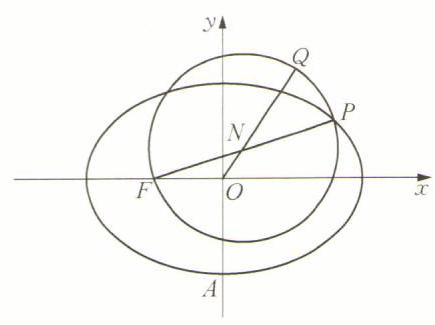
\includegraphics[width=0.3\textwidth]{bodyxb/src/bo_d1ig044601uc738hj6v0_93_1055_1304_435_325_0.jpg}
    \end{center}
    \begin{jieda}
        设 ${F}_{1}$ 为椭圆的右焦点，因为 $O$ , $N$ 分别为 $F{F}_{1}$, ${PF}$ 的中点，所以 $\left| {ON}\right|  = \dfrac{1}{2}\left| {P{F}_{1}}\right|$，$\left|{NQ}\right|  =  \dfrac{1}{2}\left| {PF}\right|$，因此$\left| {OQ}\right|  = \left| {ON}\right|  + \left| {NQ}\right|  = \dfrac{1}{2}\left( {\left| {PF}\right|  + \left| {P{F}_{1}}\right| }\right)  = 2$
        
        所以 $Q$ 的轨迹是以 $O$ 为圆心,以2为半径的圆, $A(0, - \sqrt{3})$ 在圆内，所以数形结合可知$\left| {AQ}\right|$ 的取值范围为 $\left\lbrack  {2 - \sqrt{3},2 + \sqrt{3}}\right\rbrack$ .
    \end{jieda}
    \item 在平面直角坐标系 ${xOy}$ 中,若动点 $P\left( {a,b}\right)$ 到两直线 ${l}_{1}$ : $y = x$ 和 ${l}_{2} : y =  - x + 2$ 的距离之和为 $2\sqrt{2}$ ,则 ${a}^{2} + {b}^{2}$ 的最大值是\blkda{18}.
    \begin{jieda}
        $\dfrac{|a-b|}{\sqrt{2}} + \dfrac{|a+b-2|}{\sqrt{2}} = 2\sqrt{2}$，即$|a-b| + |a+b-2| = 4$，故$P$在以$(3, 3)$，$(3, -1)$，$(-1, 3)$，$(-1, -1)$为顶点的矩形上，故$a^2+b^2 \leq 18$
    \end{jieda}
    \item 直线 $\sqrt{3}{ax} + {by} = 1\left( {a,b \in  \mathbf{R}}\right)$ 与圆 $O : {x}^{2} + {y}^{2} = 2$ 相交于 $A,B$ 两点,且 $\bigtriangleup {AOB}$ 是直角三角形 $(O$ 是坐标原点),则点 $P\left( {a,b}\right)$ 与点 $Q\left( {0,1}\right)$ 之间距离的最大值是\blkda{2}.
    \begin{jieda}
        因为$\bigtriangleup {AOB}$ 是直角三角形，$A,B$在圆上，因此只有$\angle{AOB}$可能为直角，故原点到直线 $\sqrt{3}{ax} + {by} = 1\left( {a,b \in  \mathbf{R}}\right)$的距离为$1$，即$\dfrac{1}{\sqrt{3a^2+b^2}} = 1$，所以$3a^2+b^2 = 1$，即$P$在椭圆$3x^2 + y^2 = 1$上，因此$PQ$的最大值为2
    \end{jieda}
    \item 若对圆 ${\left( x - 3\right) }^{2} + {\left( y - 2\right) }^{2} = 1$ 上任意一点 $P\left( {x,y}\right) ,\left| {{3x} - {4y} + a}\right|  + \left| {9 - {3x} + {4y}}\right|$ 的取值与 $x,y$ 无关,则实数 $a$ 的取值范围是\blkda{$[4, +\infty)$}.
    \begin{jieda}
        设$k = {3x} - {4y}$，则$\left| {{3x} - {4y} + a}\right|  + \left| {9 - {3x} + {4y}}\right| = |k+a|+|9-k|$，易知其在$[-a, 9]$或$[9, -a]$范围内值不变

        因为$P$在圆上，因此数形结合可知$k \in [-4, 6]$（相切时取得最值），故$[-4, 6] \subseteq [-a, 9]$，因此$a \geq 4$
    \end{jieda}
    \item 已知 $\sqrt{{x}^{2} + {y}^{2}} + \sqrt{{\left( x - 8\right) }^{2} + {\left( y - 6\right) }^{2}} = {20}$ ,则 $\left| {{3x} - {4y} - {100}}\right|$ 的最大值为\blkda[3]{$100+25\sqrt{3}$}.
    \begin{jieda}
        根据椭圆定义可知$\sqrt{{x}^{2} + {y}^{2}} + \sqrt{{\left( x - 8\right) }^{2} + {\left( y - 6\right) }^{2}} = {20}$对应着以$(0, 0), (8, 6)$为焦点，长轴长为$20$的椭圆

        $\left| {{3x} - {4y} - {100}}\right|$即点$(x, y)$到直线$3x - {4y} - 100 = 0$距离的5倍

        易知椭圆$\sqrt{{x}^{2} + {y}^{2}} + \sqrt{{\left( x - 8\right) }^{2} + {\left( y - 6\right) }^{2}} = {20}$的长轴与直线$3x - {4y} - 100 = 0$平行，故其最大值在椭圆短轴顶点处取到，为椭圆中心到直线距离加短半轴长的和的5倍，为$100+25\sqrt{3}$
    \end{jieda}
    \item 已知函数 $y = \dfrac{\sqrt{3}}{3}x + \dfrac{\sqrt{3}}{x}$ 的图象是双曲线, $P$ 是双曲线上任意一点, $O$ 为坐标原点,那么 ${OP}$ 的最小值是\blkda{$\sqrt{6}$}.
    \begin{jieda}
        $|OP|^2 = x^2 + \left(\dfrac{\sqrt{3}}{3}x + \dfrac{\sqrt{3}}{x}\right)^2 = x^2 + \dfrac{x^2}{3} + \dfrac{3}{x^2} + 2 = \dfrac{4x^2}{3} + \dfrac{3}{x^2} + 2 \geq 2 + 4 = 6$

        故${OP}$ 的最小值是$\sqrt{6}$
    \end{jieda}
    \item 已知定点 $A\left( {a,0}\right) \left( {a > 0}\right)$ 到椭圆 $\dfrac{{x}^{2}}{9} + \dfrac{{y}^{2}}{4} = 1$ 上的点的距离的最小值为 1,则 $a$ 的值为\blkda{2或4}.
    \begin{jieda}
        \begin{enumerate}
            \item 数形结合

            根据题意可知圆$(x-a)^2+y^2 = 1$和椭圆 $\dfrac{{x}^{2}}{9} + \dfrac{{y}^{2}}{4} = 1$相切，数形结合可知$a = 2$或$4$

            \item 代数推导

            椭圆上点$(x_0, y_0)$到$A$的距离平方为$(x_0-a)^2+y_0^2 = (x_0-a)^2 + 4 - \dfrac{4{x_0}^{2}}{9} = \dfrac{5x_0^2}{9} - 2ax_0 + a^2+4 = \dfrac{5}{9}\left(x_0 - \dfrac{9a}{5}\right)^2+4-\dfrac{4a^{2}}{5}$

            设$f(x) = \dfrac{5}{9}\left(x - \dfrac{9a}{5}\right)^2+4-\dfrac{4a^{2}}{5}, x \in [-3, 3]$
            \begin{dingautolist}{172}
                \item 当$\dfrac{9a}{5} \geq 3$，即$a \geq \dfrac{5}{3}$时，$f(x)$在$[-3, 3]$严格减，因此最小值在$x = 3$处取，$f(3) = 9-6a+a^2 = 1$，解得$a = 2$或$4$
                \item 当$a \in \left(0, \dfrac{5}{3}\right)$，则$f(x)$在$\left[-3, \dfrac{9a}{5}\right]$严格减，在$\left[\dfrac{9a}{5}, 3\right]$严格增，因此最小值在$x = \dfrac{9a}{5}$处取得最小值，$f\left(\dfrac{9a}{5}\right) = 4-\dfrac{4a^{2}}{5} = 1$，解得$a = \dfrac{\sqrt{15}}{2}$（舍）
            \end{dingautolist}
            
        \end{enumerate}
    \end{jieda}
    \item 已知椭圆方程为 $\dfrac{{x}^{2}}{2} + {y}^{2} = 1$ ,斜率为 1 的直线 $l$ 与椭圆交于 $A,B$ 两个不同的点, ${AB}$ 中点为 $Q$ ,点 $P\left( {2,0}\right)$ ,则 ${\left| PQ\right| }^{2}$ 的取值范围是\blkda[4]{$\left(\dfrac{17-8\sqrt{3}}{3}, \dfrac{17+8\sqrt{3}}{3}\right)$}.
    \begin{jieda}
        设$A(x_1, y_2), B(x_2, y_2)$，则$\left\{\begin{array}{l}
             \dfrac{{x_1}^{2}}{2} + {y_1}^{2} = 1 \\
             \dfrac{{x_2}^{2}}{2} + {y_2}^{2} = 1 
        \end{array}\right.$，两式做差可得$\dfrac{x_1^2-x_2^2}{2} + (y_1^2-y_2^2) = 0$，即$\dfrac{(x_1+x_2)(x_1-x_2)}{2} + (y_1+y_2)(y_1-y_2) = 0$，因为$\dfrac{y_1-y_2}{x_1-x_2} = 1$，所以$y_1+y_2 = -\dfrac{x_1+x_2}{2}$，即$Q$在$y = -\dfrac{x}{2}, x \in \left(-\dfrac{2\sqrt{3}}{3}, \dfrac{2\sqrt{3}}{3}\right)$上，设$Q(x, y)$，则$|PQ|^2 = (x-2)^2+y^2 = \dfrac{5}{4}x^2-4x+4$
        易知函数$f(x) = \dfrac{5}{4}x^2-4x+4$在$\left(-\dfrac{2\sqrt{3}}{3}, \dfrac{2\sqrt{3}}{3}\right)$上严格减，因此$f(x) \in \left(\dfrac{17-8\sqrt{3}}{3}, \dfrac{17+8\sqrt{3}}{3}\right)$
    \end{jieda}
    \item 已知椭圆 $\dfrac{{x}^{2}}{9} + \dfrac{{y}^{2}}{4} = 1$ 的左焦点为 $F$ ,若 $A$ 、 $B$ 是椭圆上两动点,且 ${AB}$ 垂直于 $x$ 轴,则 $\bigtriangleup  {ABF}$ 周长的最大值为\blkda{12}.
    \begin{jieda}
        根据定义数形结合可得.  
    \end{jieda}
    \item 已知椭圆 $C : \dfrac{{x}^{2}}{4} + \dfrac{{y}^{2}}{3} = 1$ 的左、右焦点分别为 ${F}_{1}\text{ 、 }{F}_{2},M$ 为椭圆 $C$ 上任意一点, $N$ 为圆 $E$ : ${\left( x - 3\right) }^{2} + {\left( y - 2\right) }^{2} = 1$ 上任意一点,则 $\left| {MN}\right|  - \left| {M{F}_{1}}\right|$ 的最小值为\blkda{$2\sqrt{2}-5$}.
    \begin{jieda}
        $\left| {MN}\right|  - \left| {M{F}_{1}}\right| = |MN| + |MF_2| - 4 \geq |ME| - 1 + |MF_2| - 4 \geq |F_2E| - 5 = 2\sqrt{2}-5$
    \end{jieda}
    \item 已知过原点的直线 $l$ 交椭圆 $\dfrac{{x}^{2}}{9} + \dfrac{{y}^{2}}{4} = 1$ 于 $P,Q$ 两点,椭圆右顶点为 $A,\bigtriangleup {APQ}$ 重心为 $G$ , $\left| {GA}\right|  + \left| {GP}\right|  + \left| {GQ}\right|$ 的取值范围是\blkda[3]{$[2\sqrt{5}+2, 8)$}.
    \begin{jieda}
        $A(3, 0)$，根据重心性质可知$G(1, 0)$，设$P(x_0, y_0)$，则$Q(-x_0, y_0)$，故$|GP|+|GQ| = \sqrt{(x_0-1)^2+y_0^2}+\sqrt{(x_0+1)^2+y_0^2}$

        当$\sqrt{(x_0-1)^2+y_0^2}+\sqrt{(x_0+1)^2+y_0^2}$等于大于2的常值时，$(x_0, y_0)$在以$(1, 0), (-1, 0)$为焦点的椭圆$\dfrac{x^2}{k}+\dfrac{y^2}{k-1} = 1$上，故数形结合可知$k \in [5, 9)$（$k = 9$时$Q$与$A$重合），即$\sqrt{(x_0-1)^2+y_0^2}+\sqrt{(x_0+1)^2+y_0^2} \in [2\sqrt{5}, 6)$

        $\left| {GA}\right|  + \left| {GP}\right|  + \left| {GQ}\right| \in [2\sqrt{5}+2, 8)$
    \end{jieda}
\end{enumerate}

\subsection*{46 面积问题}

\subsubsection*{知识点睛}

圆锥曲线题目经常会考察焦点弦三角形,焦点三角形的面积,可以用焦点三角形面积公式求解 (例如焦点在 $x$ 轴上的椭圆的焦点 $\bigtriangleup {F}_{1}P{F}_{2}$ 的面积 ${S}_{\bigtriangleup {F}_{1}P{F}_{2}} = c\left| {y}_{P}\right|  = {b}^{2}\tan \dfrac{\angle {F}_{1}P{F}_{2}}{2}$ ),其他图形面积常用切割法处理成两个三角形表示面积, 比较常见的是用坐标轴进行切割. 特别地,若四边形对角线互相垂直,长度分别为 $a,b$ ,则 $S = \dfrac{1}{2}{ab}$ ; 若 $\bigtriangleup {OAB}$ 中, $O$ 为坐标原点, $A\left( {{x}_{1},{y}_{1}}\right) ,B\left( {{x}_{2},{y}_{2}}\right)$ ,则 $S = \dfrac{1}{2}\left| {{x}_{1}{y}_{2} - {x}_{2}{y}_{1}}\right|$ .

\subsubsection*{经典习题}
\begin{enumerate}
    \item 双曲线 $\dfrac{{x}^{2}}{n} - {y}^{2} = 1\left( {n > 1}\right)$ 的两个焦点为 ${F}_{1},{F}_{2},P$ 在双曲线上,且满足 $\left| {P{F}_{1}}\right|  + \left| {P{F}_{2}}\right|  =$  $2\sqrt{n + 2}$ ,则 $\bigtriangleup P{F}_{1}{F}_{2}$ 的面积为\blkda{1}.
    \begin{jieda}
        设$t = |PF_1|, s = |PF_2|$，不妨设$t > s$，故$\left\{\begin{array}{l}
             t-s = 2\sqrt{n} \\
             t+s = 2\sqrt{n+2}
        \end{array}\right.$，故$\left\{\begin{array}{l}
             t = \sqrt{n} + \sqrt{n+2} \\
             s = \sqrt{n+2} - \sqrt{n}
        \end{array}\right.$，$|F_1F_2| = 2\sqrt{n+1}$，因为$s^2+t^2 = |F_1F_2|^2$（或利用余弦定理发现$\angle{F_1PF_2}$为直角），所以$S = \dfrac{st}{2} = 1$
    \end{jieda}
    \item 过原点 $O$ 作两条相互垂直的直线分别与椭圆 $P : \dfrac{{x}^{2}}{2} + {y}^{2} = 1$ 交于 $A\text{ 、 }C$ 与 $B\text{ 、 }D$ ,则四边形 ${ABCD}$ 面积的最小值为\dotfill{(\kh{A})}
    \xx{$\dfrac{8}{3}$}{$4\sqrt{2}$}{$2\sqrt{2}$}{$\dfrac{4}{3}$}
    \begin{jieda}
        \begin{dingautolist}{172}
            \item 当两直线分别与坐标轴平行时，$S = 2\sqrt{2}$
            \item 当两直线斜率均存在时，设$AC$为$y = kx$，与椭圆方程联立得$\left\{\begin{array}{l}
                 y = kx  \\
                 \dfrac{{x}^{2}}{2} + {y}^{2} = 1 
            \end{array}\right.$，消去$y$得到$(1+2k^2)x^2 = 2$，因此$|x_1 - x_2| = 2\sqrt{\dfrac{2}{1+2k^2}}$，则$|AC| = 2\sqrt{\dfrac{2+2k^2}{1+2k^2}}$，同理可得$|BD| = 2\sqrt{\dfrac{2+2k^2}{2+k^2}}$，故$S = \dfrac{1}{2}|AC| \cdot |BD| = 4\sqrt{\dfrac{1+k^2}{1+2k^2} \cdot \dfrac{1+k^2}{2+k^2}}$

            令$t = k^2+1, t \in [1, +\infty)$，则$S = 4\sqrt{\dfrac{t^2}{2t^2+t-1}} = \dfrac{4}{\sqrt{2+\dfrac{1}{t}-\dfrac{1}{t^2}}} \geq \dfrac{8}{3}$
        \end{dingautolist}
    \end{jieda}
    \item *已知直线 $l : x - y + 1 = 0$ 与抛物线 $C : {x}^{2} = {2y}$ 交于 $A,B$ 两点,点 $P$ 为直线 $l$ 上一动点, $M$ , $N$ 是抛物线 $C$ 上两个动点,若 $\vv{MN}//\vv{AB},\left| \vv{MN}\right|  < \left| \vv{AB}\right|$ ,则 $\bigtriangleup {PMN}$ 面积的最大值为\blkda{1}.
    \begin{jieda}
        因为$\vv{MN}//\vv{AB}$，故可设$MN: y = x + b$，联立直线和抛物线方程$\left\{\begin{array}{l}
             y = x + b \\
             x^2 = 2y
        \end{array}\right.$，消去$y$可得$x^2 - 2x - 2b = 0$，$\Delta = 4+8b > 0$，故$b > -\dfrac{1}{2}$，又因为$\left|\vv{MN}\right|  < \left| \vv{AB}\right|$，所以$b \in \left(-\dfrac{1}{2}, 1\right)$

        根据韦达定理有$\left\{\begin{array}{l}
             x_1+x_2 = 2 \\
             x_1x_2 = -2b
        \end{array}\right.$，因此$|\vv{MN}| = \sqrt{2} \cdot \sqrt{(x_1+x_2)^2-4x_1x_2} = \sqrt{2(4+8b)}$，$S_{\bigtriangleup {PMN}} = \dfrac{1}{2} \cdot \dfrac{1-b}{\sqrt{2}} \cdot \sqrt{2(4+8b)} = (1-b)\sqrt{1+2b}$

        设$f(x) = (2x+1)(x-1)^2$，则$f'(x) = 2(x-1)^2 + 2(x-1)(2x+1) = 6x(x-1)$，当$x \in \left(-\dfrac{1}{2}, 0\right)$时，$f(x)$严增，当$x \in (0, 1)$时，$f(x)$严减，因此$f(x)$在$x = 0$处取得最大值，即$S_{\bigtriangleup {PMN}} \leq 1$
    \end{jieda}
    \item 设 $m,n \in  \mathbf{R}$ ,若直线 ${mx} + {ny} - 1 = 0$ 与 $x$ 轴相交于点 $A$ ,与 $y$ 轴相交于点 $B$ ,且 $l$ 与圆 ${x}^{2} +$  ${y}^{2} = 4$ 相交所得弦的长为 2, $O$ 为坐标原点,则 $\bigtriangleup  {ABO}$ 面积的最小值为\dotfill{(\kh{A})}
    \xx{3}{4}{2}{$\sqrt{2}$}
    \begin{jieda}
        $\triangle ABO$为直角三角形，$O$到$AB$的距离为$\sqrt{3}$，故当$|AB|$最小时，$S_{\triangle ABO}$取最小

        设$P$在$AB$上，且$OP \perp AB$，故$|OP| = \sqrt{3}$，根据相似三角形可知$|AP| \cdot |BP| = 3$，根据基本不等式可知$|AP| + |BP| \geq 2\sqrt{3}$，因此$S \geq 3$
    \end{jieda}
    \item 设 ${F}_{1},{F}_{2}$ 为椭圆 $\dfrac{{x}^{2}}{4} + \dfrac{{y}^{2}}{3} = 1$ 的左、右焦点,过椭圆中心任作一条直线与椭圆交于 $P,Q$ 两点,当四边形 $P{F}_{1}Q{F}_{2}$ 面积最大时, $\vv{P{F}_{1}} \cdot  \vv{P{F}_{2}}$ 的值等于\blkda{2}.
    \begin{jieda}
        由对称性可知$S_{P{F}_{1}Q{F}_{2}} = 2S_{\triangle PF_1F_2}$，故易知$P$为短轴顶点时取得最大值，因此$\vv{PF_1} \cdot \vv{PF_2} = 2$
    \end{jieda}
    \item 设 ${AB}$ 是过椭圆 $\dfrac{{x}^{2}}{{a}^{2}} + \dfrac{{y}^{2}}{{b}^{2}} = 1\left( {a > b > 0}\right)$ 中心的弦,椭圆的左焦点为 ${F}_{1}\left( {-c,0}\right)$ ,若 $\bigtriangleup {F}_{1}{AB}$ 的面积的最大值为 2,则所有符合要求的椭圆中, $\left| {A{F}_{1}}\right|  + \left| {B{F}_{1}}\right|$ 的最小值是\blkda{4}.
    \begin{jieda}
        $S_{\bigtriangleup {F}_{1}{AB}} = \dfrac{1}{2} \times c \times |y_A - y_B|$，故当$AB$为短轴时面积最大，即$bc = 2$
        
        根据对称性可知$\left| {A{F}_{1}}\right|  + \left| {B{F}_{1}}\right| = 2a$. 因为$a^2 = b^2+c^2 \geq 2bc = 4$，所以$2a$最小值为$4$.
    \end{jieda}
    \item 已知圆 $M : {x}^{2} + {y}^{2} - {2x} - {2y} - 2 = 0$ ,直线 $l : {2x} + y + 2 = 0,P$ 为 $l$ 上的动点,过点 $P$ 作圆 $M$ 的切线 ${PA}$ 、 ${PB}$ ,切点为 $A$ 、 $B$ ,当四边形 ${PAMB}$ 面积最小时,直线 ${AB}$ 的方程为 \dotfill{(\kh{D})}
    \xx{${2x} - y - 1 = 0$}{${2x} + y - 1 = 0$}{${2x} - y + 1 = 0$}{${2x} + y + 1 = 0$}
    \begin{jieda}
        数形结合易知当$PM$最短的时候，四边形 ${PAMB}$ 面积最小，此时$P(-1, 0)$，故$AB$的方程为$(x-1)(-1-1) + (y-1)(0-1) = 4$，即${2x} + y + 1 = 0$
    \end{jieda}
    \item 在平面直角坐标系 ${xOy}$ 中,已知点 $P\left( {3,0}\right)$ 在圆 $C : {x}^{2} + {y}^{2} - {2mx} - {4y} + {m}^{2} - {28} = 0$ 内, 动直线 ${AB}$ 过点 $P$ 且交圆 $C$ 于 $A,B$ 两点,若 $\bigtriangleup {ABC}$ 的面积的最大值为 16,则实数 $m$ 的取值范围为\blkda[8]{$ (3-2\sqrt{7}, 3-2\sqrt{3}] \cup [3+2\sqrt{3}, 3+2\sqrt{7})$}.
    \begin{jieda}
        将圆化为标准方程有$(x-m)^2+(y-2)^2 = 32$，半径为$4\sqrt{2}$，故根据三角形面积公式可知：
        \begin{dingautolist}{172}
            \item 面积最大时，圆心角为直角，对应的弦长$AB$为$8$
            \item 该面积是所有满足条件的三角形中面积最大的，因此只要能够取得对应的弦长即可
        \end{dingautolist}
        因此只要$C$到圆心的距离大于等于4即可，又因为$C$在圆内，故$32 \geq (m-3)^2 + 4 \geq 16$，即$m \in (3-2\sqrt{7}, 3-2\sqrt{3}] \cup [3+2\sqrt{3}, 3+2\sqrt{7})$
    \end{jieda}
    \item 已知 ${AC},{BD}$ 为圆 ${x}^{2} + {y}^{2} = {16}$ 的两条相互垂直的弦,垂足为 $M\left( {1,2}\right)$ ,则四边形 ${ABCD}$ 面积的最大值为\blkda{27}.
    \begin{jieda}
        圆 ${x^2} + {y^2} = {16}$ 的圆心坐标为 $O\left( {0,0}\right)$ ,半径为4,设圆心 $O$ 到 ${AC}\text{、}{BD}$ 的距离分别为 ${d}_{1}\text{、}{d}_{2}$ ,因为垂足为 $M\left( {1,2}\right)$ ,所以${d}_1^2 + {d}_2^2 = O{M}^{2} = {1}^{2} + {2}^{2} = 5$ ,所以四边形ABCD的面积 $S = \dfrac{1}{2}\left| {AB}\right|  \cdot  \left| {CD}\right|  = 2\sqrt{\left( {{16} - {d}_{1}^{2}}\right) \left( {{16} - {d}_{2}^{2}}\right) } \leq  {32} - \left( {{d}_{1}^{2} + {d}_{2}^{2}}\right)  = 27$ ,当且仅当${d}_{1}^2 = {d}_{2}^2$ 时等号成立.
    \end{jieda}
    \item 过圆 $C : {\left( x - 1\right) }^{2} + {\left( y - 1\right) }^{2} = 1$ 的圆心,作直线分别交 $x$ 、 $y$ 正半轴于点 $A$ 、 $B,\bigtriangleup {AOB}$ 被圆分成四部分 (如图),若这四部分图形面积满足 ${S}_{{I}} + {S}_{{IV}} = {S}_{{{II}}} + {S}_{{{III}}}$ ,则直线 ${AB}$ 有\dotfill{(\kh{B})}

    \begin{center}
    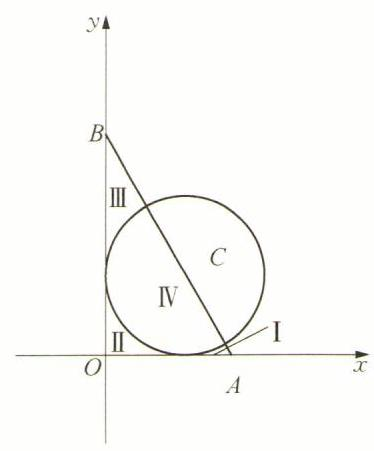
\includegraphics[width=0.3\textwidth]{bodyxb/src/bo_d1ig044601uc738hj6v0_96_1146_943_374_451_0.jpg}
    \end{center}
    
    \xx{0 条}{1 条}{2 条}{3 条}
    \begin{jieda}
        易知随着$AB$倾斜程度减小，${S}_{{{III}}}$从无穷大一直减小到0，${S}_{{I}}$从0一直增大到无穷大，而${S}_{{II}}, {S}_{{IV}}$不变，故满足条件的直线仅有一条
    \end{jieda}
    \item *自抛物线 ${y}^{2} = {4x}$ 上一点 $A\left( {1,2}\right)$ 引两弦 ${AM}\text{ 、 }{AN}$（$A$在$M,N$上方） ,已知两弦的斜率之和为零, $\bigtriangleup  {AMN}$ 面积的最大值是\blkda{$\dfrac{32\sqrt{3}}{9}$}.
    \begin{jieda}
        $k_{MN} = -1$
        
        推导如下：设$M\left( {{x}_{1},{y}_{1}}\right) ,N\left( {{x}_{2},{y}_{2}}\right)$，则${k}_{1} = \dfrac{{y}_{1} - 2}{{x}_{1} - 1} = \dfrac{{y}_{1} - 2}{\dfrac{{y}_{1}^{2}}{4} - 1} = \dfrac{4}{{y}_{1} + 2}$ ,同理可得 ${k}_{2} = \dfrac{{y}_{2} - 2}{{x}_{2} - 1} = \dfrac{4}{{y}_{2} + 2}$. 
        由 ${k}_{1} + {k}_{2} = 0$ ,得 $\dfrac{4}{{y}_{1} + 2} + \dfrac{4}{{y}_{2} + 2} = 0$ ,即 ${y}_{1} + {y}_{2} + 4 = 0$. 
        设直线 $MN$ 的方程为 $x = {m}y + {t}$ ,联立抛物线方程可得 ${y^2} - 4{m}y - 4{t} = 0$. 
        则 $\Delta  > 0, \left\{\begin{array}{l}
             {y}_{1} + {y}_{2} = 4{m}  \\
             {y}_{1}{y}_{2} =  - 4{t} 
        \end{array}\right.$ 代入${y}_{1} + {y}_{2} + 4 = 0$可得 $4{m} + 4 = 0,{m} =  - 1$
        
        即$k_{MN} = -1$，$MN: x + y - {t} = 0$，$16+16t > 0, \left\{\begin{array}{l}
             {y}_{1} + {y}_{2} = -4  \\
             {y}_{1}{y}_{2} =  -4{t} 
        \end{array}\right.$

        $A$到$MN$的距离为$d = \dfrac{|3-t|}{\sqrt{2}}$，故$S = \dfrac{1}{2} \times \dfrac{|3-t|}{\sqrt{2}} \times \sqrt{2}|y_1-y_2| = \dfrac{1}{2} \times |3-t| \times \sqrt{16+16t}$

        $S^2 = 4(3-t)^2(1+t)$，设$f(x) = 4(x-3)^2(1+x), x > -1$，$f'(x) = 8(x-3)(1+x) + 4(x-3)^2 = 4(x-3)(3x-1)$，故$f(x)$在$x = \dfrac{1}{3}$处取得最大值，即$S^2 \leq \dfrac{1024}{27}$，故$S \leq \dfrac{32\sqrt{3}}{9}$
    \end{jieda}
    \item 设 $a\text{ 、 }b$ 是两个实数,且满足 $0 \leq  a < b$ ,直线 $l : y = {kx} + m$ 和圆 ${x}^{2} + {y}^{2} = 1$ 交于两点 $A\text{ 、 }B$ ,若存在正数 $m$ ,对于任意的 $k \in \left\lbrack  {a,b}\right\rbrack$ ,均使得 $\bigtriangleup {OAB}$ 的面积不小于 $\dfrac{\sqrt{3}}{4}$ ,则 $b - {2a}$ 的最大值为\blkda{$\sqrt{2}$}.
    \begin{jieda}
        设 $O$ 到直线 $l$ 的距离为 $d$ ,则${S}_{\bigtriangleup {AOB}} = \dfrac{1}{2} \times  2\sqrt{1 - {d}^{2}} \times  d \geq  \dfrac{\sqrt{3}}{4}$，解得 $\dfrac{1}{2} \leq  d \leq  \dfrac{\sqrt{3}}{2}$，即 $\dfrac{1}{2} \leq  \dfrac{m}{\sqrt{{k}^{2} + 1}} \leq  \dfrac{\sqrt{3}}{2}$，所以$\dfrac{1}{2}\sqrt{{k}^{2} + 1} \leq  m \leq  \dfrac{\sqrt{3}}{2}\sqrt{{k}^{2} + 1}$，若存在正数 $m$，对于任意的 $k \in \left\lbrack  {a,b}\right\rbrack$均满足要求，则应有${\left( \dfrac{1}{2}\sqrt{{k}^{2} + 1}\right) }_{\text{max }} \leq m \leq {\left( \dfrac{\sqrt{3}}{2}\sqrt{{k}^{2} + 1}\right) }_{\text{min }}$

        因为$\left\{\begin{array}{l}
             {\left( \dfrac{1}{2}\sqrt{{k}^{2} + 1}\right) }_{\text{max }} = \dfrac{1}{2}\sqrt{{b}^{2} + 1}  \\
             {\left( \dfrac{\sqrt{3}}{2}\sqrt{{k}^{2} + 1}\right) }_{\text{min }} = \dfrac{\sqrt{3}}{2}\sqrt{{a}^{2} + 1} 
        \end{array}\right.$，所以应有$\dfrac{1}{2}\sqrt{{b}^{2} + 1} \leq  \dfrac{\sqrt{3}}{2}\sqrt{{a}^{2} + 1}$ ,化简得$\dfrac{{b}^{2}}{2} - \dfrac{3{a}^{2}}{2} \leq  1$ ,且 $0 \leq  a < b$
        \begin{center}
            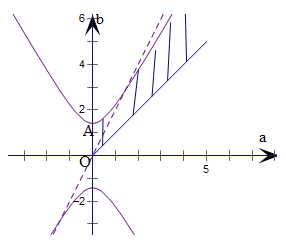
\includegraphics[width=0.4\linewidth]{bodyxb//src/46-12.png}
        \end{center}
        设 $b - {2a} = t$ ,即 $b = {2a} + t$，在平面直角坐标系 $a - O - b$ 中,直线$b = {2a} + t$ 和由 $\dfrac{{b}^{2}}{2} - \dfrac{3{a}^{2}}{2} \leq  1$，且 $0 \leq  a < b$ 表示的平面区域有公共点
        
        当直线 $b = {2a} + t$ 经过点 $A(0$ , $\sqrt{2})$ 时, $t$最大, ${t}_{max} = \sqrt{2}$ .
    \end{jieda}
    \item 已知 $A,B,C$ 是椭圆 $\dfrac{{x}^{2}}{12} + \dfrac{{y}^{2}}{4} = 1$ 上三个不同的点, $\bigtriangleup  {ABC}$ 的重心为原点 $O$ ,那么 $\bigtriangleup  {ABC}$ 的面积是\blkda{9}.
    \begin{jieda}
        设$A(2\sqrt{3}cos\alpha, 2sin\alpha)$，$B(2\sqrt{3}cos\beta, 2sin\beta)$，因为$O$是$\bigtriangleup  {ABC}$ 的重心，所以$C(-2\sqrt{3}(cos\alpha + cos\beta), -2(sin\alpha+sin\beta))$，因为$C$在椭圆上，所以$(cos\alpha + cos\beta)^2+(sin\alpha+sin\beta)^2 = 1$，即$1+2cos(\alpha-\beta) = 0$，故$cos(\alpha - \beta) = -\dfrac{1}{2}$

        $S = 3 \times \dfrac{1}{2} \times 4\sqrt{3}|cos\alpha sin\beta - sin\alpha cos\beta| = 6\sqrt{3}|sin(\beta-\alpha)| = 6\sqrt{3} \times \dfrac{\sqrt{3}}{2} = 9$

    \end{jieda}
\end{enumerate}
\section*{数列}

数列是非常有趣的数字游戏, 可以通过观察、演绎推理和归纳猜测找出特定数列的规律和性质, 也可以反过来通过数列的规律和性质, 研究特定的问题. 数列是高中阶段为数不多的刻画离散现象的数学模型,对于我们进一步理解函数的概念有重要的意义. 同时数列和我们的生活联系紧密, 很多现实问题都可以用数列的知识建模解决. 在高考试题中, 数列题目有很多经典的解题方法, 是有必要整理记忆的.

\subsection*{47 数列的概念}

\subsubsection*{知识点睛}

数列是按照一定规律排列的一列数字,同时,数列还是一种特殊的函数,其特殊性主要表现在其定义域和值域上. 在涉及数列概念的相关题目时, 我们可以由特殊到一般, 演绎推理, 归纳找出规律,也可以利用函数的思想来解决问题——函数所具备的很多性质,数列也都具备, 比如高中阶段要求掌握的单调性、奇偶性、周期性在一些数列里都有体现.

\subsubsection*{经典习题}
\begin{enumerate}
    \item *若整数数列 ${a}_{1},{a}_{2},\cdots ,{a}_{10}$ 满足 ${a}_{10} = 3{a}_{1},{a}_{2} + {a}_{8} = 2{a}_{5}$ ,且 ${a}_{i + 1} \in  \left\{  {1 + {a}_{i},2 + {a}_{i}}\right\}  ,i =$  $1,2,\cdots ,9$ ,则这样的数列的个数为\blkda{80}.
    \begin{jieda}
        设 ${b}_{i} = {a}_{i + 1} - {a}_{i} \in  \{ 1,2\} \left( {i = 1,2,\cdots ,9}\right)$
        
        则有
        $\left\{\begin{array}{l}
             2{a}_{1} = {a}_{10} - {a}_{1} = {b}_{1} + {b}_{2} + \cdots  + {b}_{9}  \\
             {b}_{2} + {b}_{3} + {b}_{4} = {a}_{5} - {a}_{2} = {a}_{8} - {a}_{5} = {b}_{5} + {b}_{6} + {b}_{7}
        \end{array}\right.$ 
        
        用 $t$ 表示 ${b}_{2}$ 、 ${b}_{3}$ 、 ${b}_{4}$ 中值为 2 的项数，由下式可知, $t$ 也是 ${b}_{5}$ 、 ${b}_{6}$ 、 ${b}_{7}$ 中值为 2 的项数,其中
        $t \in  \{ 0,1,2,3\} ,$
        所以 ${b}_{2},{b}_{3},\cdots ,{b}_{7}$ 的取法数为 ${\left( {{C}}_{3}^{0}\right) }^{2} + {\left( {{C}}_{3}^{1}\right) }^{2} + {\left( {{C}}_{3}^{2}\right) }^{2} + {\left( {{C}}_{3}^{3}\right) }^{2} = {20}$
        
        取定 ${b}_{2},{b}_{3},\cdots ,{b}_{7}$ 后,任
        意指定 ${b}_{8}$ 、 ${b}_{9}$ 的值,有 ${2}^{2} = 4$ 种方式。
        由上式可知，应取 ${b}_{1} \in  \{ 1,2\}$ 使得 ${b}_{1} + {b}_{2} + \cdots  + {b}_{9}$ 为偶数,而这样的 ${b}_{1}$ 的取法是唯一的，并且
        确定了整数 ${a}_{1}$ 的值,进而数列 ${b}_{1},{b}_{2},\cdots ,{b}_{9}$ 唯一对应一个满足条件的数列 ${a}_{1},{a}_{2},\cdots ,{a}_{10}$

        
        综上可知,满足条件的数列的个数为 ${20} \times  4 = {80}$ 
    \end{jieda}
    \item 设数列 ${a}_{1},{a}_{2},{a}_{3},{a}_{4}$ 各项互不相同,且 ${a}_{i} \in  \{ 1,2,3,4\} \left( {i = 1,2,3,4}\right)$ . 若下列四个关系: \ding{172}${a}_{1} = 1$ ；\ding{173} ${a}_{2} \neq  1$ ；\ding{174}${a}_{3} = 2$ ；\ding{175} ${a}_{4} \neq  4$ 中恰有一个正确,则 $\left( {{10}{a}_{1} + {a}_{2}}\right)  - \left( {{10}{a}_{3} + {a}_{4}}\right)$ 的最大值是\blkda{18}.
    \begin{jieda}
        \begin{dingautolist}{172}
            \item 仅\ding{172}正确无解
            \item 仅\ding{173}正确时最优情况：$a_1 = 3, a_2 = 2, a_3 = 1, a_4 = 4$，$\left( {{10}{a}_{1} + {a}_{2}}\right)  - \left( {{10}{a}_{3} + {a}_{4}}\right) = 18$
            \item 仅\ding{174}正确时最优情况：$a_1 = 3, a_2 = 1, a_3 = 2, a_4 = 4$，$\left( {{10}{a}_{1} + {a}_{2}}\right)  - \left( {{10}{a}_{3} + {a}_{4}}\right) = 7$
            \item 仅\ding{174}正确时最优情况：$a_1 = 4, a_2 = 1, a_3 = 3, a_4 = 2$，$\left( {{10}{a}_{1} + {a}_{2}}\right)  - \left( {{10}{a}_{3} + {a}_{4}}\right) = 9$
        \end{dingautolist}
    \end{jieda}
    \item $\left\{  {a}_{n}\right\}$ 是由实数构成的无穷等比数列, ${S}_{n} = {a}_{1} + {a}_{2} + \cdots  + {a}_{n}$ ,关于数列 $\left\{  {S}_{n}\right\}$ ,给出下列命题: 
    \begin{dingautolist}{172}
        \item 数列 $\left\{  {S}_{n}\right\}$ 中任意一项均不为 0
        \item 数列 $\left\{  {S}_{n}\right\}$ 中必有一项为 0
        \item 数列中或者任意一项不为 0,或者有无穷多项为 0
        \item 数列 $\left\{  {S}_{n}\right\}$ 中一定不可能出现 ${S}_{n} = {S}_{n + 2}$
        \item 数列 $\left\{  {S}_{n}\right\}$ 中一定不可能出现 ${S}_{n} = {S}_{n + 3}$
    \end{dingautolist}
    其中正确的命题是\dotfill{(\kh{C})}
    \xx{\ding{172}\ding{174}}{\ding{173}\ding{175}}{\ding{174}\ding{176}}{\ding{173}\ding{176}}
    \begin{jieda}
        $S_n = \left\{\begin{array}{ll}
             na_1, & q = 1 \\
             \dfrac{a_1(1-q^n)}{1-q}, & q \neq 1
        \end{array}\right.$，可知当$q = -1$时$S_n$中存在无数项为0，$q \neq -1$时$S_n$中不存在0，故\ding{172}\ding{173}错误，\ding{174}正确

        当$q = -1$时存在${S}_{n} = {S}_{n + 2}$，故\ding{175}错误

        $q = 1$时易知不可能有$S_n = S_{n+3}$，当$q \neq 1$时，$q^3 = 1$无实数解，因此不可能有$S_n = S_{n+3}$，因此\ding{176}正确
    \end{jieda}
    \item 已知数列 $\left\{  {a}_{n}\right\}$ 的首项为 4,且满足 $2\left( {n + 1}\right) {a}_{n} - n{a}_{n + 1} = 0\left( {n \in  {\mathbf{N}}^{ * }}\right)$ ,则下列命题: 
    \begin{dingautolist}{172}
        \item $\left\{  \dfrac{{a}_{n}}{n}\right\}$ 是等差数列
        \item $\left\{  {a}_{n}\right\}$ 是递增数列
        \item 设函数 $f\left( x\right)  = x - \dfrac{1}{2} - {\left( \dfrac{{a}_{n}}{{a}_{n + 1}}\right) }^{x - 2}$ ,则存在某个区间 $\left( {n,n + 1}\right) \left( {n \in  {\mathbf{N}}^{ * }}\right)$ ,使得 $f\left( x\right)$ 在 $\left( {n,n + 1}\right)$ 上有唯一零点
    \end{dingautolist}
    则其中正确的命题序号为\blkda{\ding{173}\ding{174}}.
    \begin{jieda}
        \begin{dingautolist}{172}
            \item $\left\{  \dfrac{{a}_{n}}{n}\right\}$ 是公比为2的等比数列
            \item $a_n = n \cdot 2^{n+1}$
            \item $f(x) = x - \dfrac{1}{2} - \left(\dfrac{n}{2(n+1)}\right)^{x-2}$，因为$\dfrac{n}{2(n+1)} \in \left(0, \dfrac{1}{2}\right)$，所以$f(x)$严格增，存在唯一零点.

            当$n = 1$时，根据零点存在定理可知$f(x)$在$(1, 2)$内存在零点，满足要求.
        \end{dingautolist}
    \end{jieda}
    \item 在数列 $\left\{  {a}_{n}\right\}$ 中,若存在非零整数 $T$ ,使得 ${a}_{m + T} = {a}_{m}$ 对于任意的正整数 $m$ 均成立,那么称数列 $\left\{  {a}_{n}\right\}$ 为周期数列,其中 $T$ 叫做数列 $\left\{  {a}_{n}\right\}$ 的周期,若数列 $\left\{  {x}_{n}\right\}$ 满足 ${x}_{n + 1} = \left| {{x}_{n} - {x}_{n - 1}}\right|$  $\left( {n \geq  2,n \in  \mathbf{N}}\right)$ ,如 ${x}_{1} = 1,{x}_{2} = a\left( {a \in  \mathbf{R},a \neq  0}\right)$ ,当数列 $\left\{  {x}_{n}\right\}$ 的周期最小时,该数列的前 2021 项的和为\dotfill{(\kh{D})}
    \xx{673}{674}{1346}{1348}
    \begin{jieda}
        若$x_2 = 1$，则$x_n$为：$1,1,0,1,1,0,\cdots $，周期为三，易知该数列不为常数列，因此考虑是否可能周期为2

        若周期为2，则$x_3 = 1$，$x_2 = 0$或$2$，则$x_4 = 1$，与周期为2矛盾

        因此周期最小时，$x_n$为：$1,1,0,1,1,0,\cdots $
    \end{jieda}
    \item 下列命题:
    \begin{dingautolist}{172}
        \item “ $0 < a \leq  \dfrac{1}{2}$ ” 是 “存在 $n \in  {\mathbf{N}}^{ * }$ ,使得 ${\left( \dfrac{1}{2}\right) }^{n} = a$ 成立” 的充分条件
        \item “ $a > 0$ ” 是 “存在 $n \in  {\mathbf{N}}^{ * }$ ,使得 ${\left( \dfrac{1}{2}\right) }^{n} < a$ 成立” 的必要条件
        \item “ $a > \dfrac{1}{2}$ ” 是 “不等式 ${\left( \dfrac{1}{2}\right) }^{n} < a$ 对一切 $n \in  {\mathbf{N}}^{ * }$ 恒成立”的充要条件.
    \end{dingautolist}
    其中为真命题的序号是\dotfill{(\kh{B})}
    \xx{\ding{174}}{\ding{173}\ding{174}}{\ding{172}\ding{173}}{\ding{172}\ding{174}}
    \item 设 $\left\{  {a}_{n}\right\}$ 是 2022 项的实数数列, $\left\{  {a}_{n}\right\}$ 中的每一项都不为零, $\left\{  {a}_{n}\right\}$ 中任意连续 11 项 ${a}_{n}$ , ${a}_{n + 1},\cdots ,{a}_{n + {10}}$ 的乘积是定值 $\left( {n = 1,2,3,\cdots ,{2022}}\right)$ ,则命题:
    \begin{dingautolist}{172}
        \item 存在满足条件的数列, 使得其中恰有 365 个 1
        \item 不存在满足条件的数列, 使得其中恰有 550 个 1
    \end{dingautolist}
    的真假情况为\dotfill{(\kh{D})}
    \xx{\ding{172}和\ding{173}都是真命题}{\ding{17\ding{173}}是真命题,\ding{173}是假命题}{\ding{173}是真命题,\ding{172}是假命题}{\ding{172}\ding{173}都是假命题}
    \begin{jieda}
        易知$a_n$的周期为11，$2022$项为$183$个周期，且余9项
        
        $365 \div 183 = 1 \cdots 182$，若每个周期有一个1，则还差182个1，若每个周期有2个1，则会超过365个1，因此不存在满足条件的数列

        $550 \div 183 = 3 \cdots 1$，因此只需每个周期内的后三项为1即可满足要求.
    \end{jieda}
    \item 有一个三人报数游戏:首先 $A$ 报数字 1,然后 $B$ 报下两个数字 2,3,接下来 $C$ 报下三个数字 4,5,6,然后轮到 $A$ 报下四个数字 7,8,9,10,依次循环,直到报出 10000,则 $A$ 报出的第 2021 个数字为\dotfill{(\kh{C})}
    \xx{5979}{5980}{5981}{以上都不对}
    \begin{jieda}
        $A$报数的数字个数构成的数列为$1$为首项，$3$为公差的等差数列，故其前$n$项和$T_n = \dfrac{n(3n-1)}{2}$，$T_{37} = 2035, T_{36} = 1926$，故$A$在第37轮中报出的109个数字中的第95个数字是目标数字

        易知三个人报数结束的尾数为1为首项，1为公差的等差数列的前$n$项和$S_n = \dfrac{n(n+1)}{2}$，36轮结束后$C$所报尾数为$S_{108} = 5886$，故目标数字为$5886+95 = 5981$
    \end{jieda}
    \item 已知数列 $\left\{  {a}_{n}\right\}$ 满足: ${a}_{1} = 1,{a}_{n + 1} - {a}_{n} \in  \left\{  {{a}_{1},{a}_{2},\cdots ,{a}_{n}}\right\}  \left( {n \in  {\mathbf{N}}^{ * }}\right)$ ,记数列 $\left\{  {a}_{n}\right\}$ 的前 $n$ 项和为 ${S}_{n}$ . 若对所有满足条件的 $\left\{  {a}_{n}\right\}  ,{S}_{10}$ 的最大值为 $M$ ,最小值为 $m$ ,则 $M + m =$ \blkda{1078}.
    \begin{jieda}
        易知$a_n$为严增数列
        \begin{dingautolist}{172}
            \item $S_n$最大，即$a_n$在前十项增长最快，$a_n = 2^{n-1}$，$S_{10} = 1023$
            \item $S_n$最小，即$a_n$在前十项增长最慢，$a_n = n$，$S_{10} = 55$
        \end{dingautolist}
        因此$M + m = 1023 + 55 = 1078$
    \end{jieda}
    \item * 设 ${a}_{1},{a}_{2},{a}_{3},{a}_{4} \in  \mathbf{R}$ ,且 ${a}_{1}{a}_{4} - {a}_{2}{a}_{3} = 1$ ,则代数式 ${a}_{1}^{2} + {a}_{2}^{2} + {a}_{3}^{2} + {a}_{4}^{2} + {a}_{1}{a}_{3} + {a}_{2}{a}_{4}$ 的最小值为\blkda{$\sqrt{3}$}.
    \begin{jieda}
        设 $\vv{OA} = \vv{a} = \left( {{a}_{1},{a}_{2}}\right) ,\vv{OB} = \vv{b} = \left( {{a}_{3},{a}_{4}}\right)$，设 $\vv{a},\vv{b}$ 的夹角为 $\theta ,{a}_{1}{a}_{4} - {a}_{2}{a}_{3} = 1,\vv{a},\vv{b}$ 不共线, $0 < \theta  < \pi$ .
        
        ${a}_{1}{a}_{4} - {a}_{2}{a}_{3} = 1$即以$\vv{a}, \vv{b}$为邻边的平行四边形面积为1，即$|\vv{a}|\cdot|\vv{b}|sin\theta = 1$
        
        故$2\left| \vv{a}\right| |\vv{b}|  + \vv{a} \cdot  \vv{b} = \dfrac{2}{\sin \theta } + \dfrac{\cos \theta }{\sin \theta } = \dfrac{\cos \theta  + 2}{\sin \theta }$ ①
        设 $M\left( {\sin \theta ,\cos \theta }\right)$ , $\left( {0 < \theta  < \pi }\right)$ , $P\left( {0, - 2}\right)$ ,①式表示点 $P\left( {0, - 2}\right)$ 与单位圆( $y$ 轴右侧)的点 $M$ 连线斜率,当 ${PM}$ 与单位圆相切的时斜率最小为 $\sqrt{3}$
    \end{jieda}
    \item 设数列 $\left\{  {a}_{n}\right\}$ 是首项为 0 的递增数列, ${f}_{n}\left( x\right)  = \left| {\sin \dfrac{1}{n}\left( {x - {a}_{n}}\right) }\right| ,x \in  \left\lbrack  {{a}_{n},{a}_{n + 1}}\right\rbrack  (n \in$  $\left. {\mathbf{N}}^{ * }\right)$ ,满足: 对于任意的 $b \in  \lbrack 0,1),{f}_{n}\left( x\right)  = b$ 总有两个不同的根,则 $\left\{  {a}_{n}\right\}$ 的通项公式为\blkda[3]{$a_n = \dfrac{n(n-1)}{2}\pi$}.
    \begin{jieda}
        为满足对于任意的 $b \in  \lbrack 0,1),{f}_{n}\left( x\right)  = b$ 总有两个不同的根，应有$a_{n+1}$与$a_n$的差为半个周期，即$a_{n+1} = a_n + n\pi$，故$a_n = \dfrac{n(n-1)}{2}\pi$
    \end{jieda}
\end{enumerate} 

\subsection*{48 等差等比数列}

\subsubsection*{知识点睛}

1. 等差等比数列不光要记忆等差、等比数列的各种计算公式, 也要从数列的对称性、等量 (率)增长等角度理解数列,等差数列是离散的线性函数,等比数列是类指数函数,善用函数化处理技巧, 对公式的结构进行分析.

2. 提醒大家几个可能被忽略但是很实用的性质:

(1)等差数列任意两项间的关系:如果 ${a}_{n}$ 是等差数列的第 $n$ 项, ${a}_{m}$ 是等差数列的第 $m$ 项, 且 $m \leq  n$ ,公差为 $d$ ,则有 ${a}_{n} = {a}_{m} + \left( {n - m}\right) d$ ；

(2)对于等差数列 $\left\{  {a}_{n}\right\}$ ,若 $n + m = p + q$ ,则 ${a}_{n} + {a}_{m} = {a}_{p} + {a}_{q}$ ；

(3)若数列 $\left\{  {a}_{n}\right\}$ 是等差数列, ${S}_{n}$ 是其前 $n$ 项的和, $k \in  {{N}}^{ * }$ ,那么 ${S}_{k},{S}_{2k} - {S}_{k},{S}_{3k} - {S}_{2k}$ 成等差数列;

(4)等差数列公差为 $d$ ,若 $d > 0$ ,则数列递增；若 $d < 0$ ,则数列递减；若 $d = 0$ ,则数列为常数列;

(5)等比数列的常用性质和等差数列有类比对应关系,如:若 $\left\{  {a}_{n}\right\}$ 是等比数列,且 $m + n =$  $p + q\left( {m,n,p,q \in  {\mathbf{N}}^{ * }}\right)$ ,则 ${a}_{n} \cdot  {a}_{m} = {a}_{p} \cdot  {a}_{q}$ ,特别地,当 $m + n = {2k}$ 时, ${a}_{m} \cdot  {a}_{n} = {a}_{k}^{2}$ .

\subsubsection*{经典习题}
\begin{enumerate}
    \item 无穷等差数列 $\left\{  {a}_{n}\right\}$ 的首项为 ${a}_{1}$ ,公差为 $d$ ,前 $n$ 项和为 ${S}_{n}\left( {n \in  {{N}}^{ * }}\right.$ ),则 “ ${a}_{1} + d > 0$ ” 是 “ $\left\{  {S}_{n}\right\}$ 为递增数列”的\dotfill{(\kh{B})}
    \xx{充分非必要条件}{必要非充分条件}{充要条件}{既非充分也非必要条件}
    \begin{jieda}
        $S_n$递增则应从第二项起均为正，因此可以推出$a_2 = a_1+d > 0$，但$a_2 > 0$不代表$S_n$递增，比如$a_n = 3-2n$
    \end{jieda}
    \item 已知等比数列 $\left\{  {a}_{n}\right\}$ 的前 $n$ 项积为 ${T}_{n}$ ,若 ${a}_{1} =  - {24},{a}_{4} =  - \dfrac{8}{9}$ ,则当 ${T}_{n}$ 取最大值时, $n$ 的值为\blkda{4}.
    \begin{jieda}
        根据${a}_{1} =  - {24},{a}_{4} =  - \dfrac{8}{9}$可知$q = \dfrac{1}{3}$，故$a_n = -72 \left(\dfrac{1}{3}\right)^n$

        故可知$T_n$正负交替，$|T_n|$在$n \leq 3$时严增，在$n > 4$时严减，因此$T_n$最大值应为$T_2$或$T_4$

        因为$T_4 = T_2 \times \left(-\dfrac{8}{3}\right) \times \left(-\dfrac{8}{9}\right) > T_2$，所以$T_4$为最大值.
    \end{jieda}
    \item 已知 ${a}_{1}$ 、 ${a}_{2}$ 、 ${a}_{3}$ 、 ${a}_{4}$ 是各项均为正数的等差数列,其公差 $d$ 大于零,若线段 ${l}_{1}$ 、 ${l}_{2}$ 、 ${l}_{3}$ 、 ${l}_{4}$ 的长分别为 ${a}_{1}$ 、 ${a}_{2}$ 、 ${a}_{3}$ 、 ${a}_{4}$ ,则\dotfill{(\kh{C})}
    \xx{对任意的 $d$ ,均存在以 ${l}_{1}$ 、 ${l}_{2}$ 、 ${l}_{3}$ 为三边的三角形}{对任意的 $d$ ,均不存在以 ${l}_{1}$ 、 ${l}_{2}$ 、 ${l}_{3}$ 为三边的三角形}{对任意的 $d$ ,均存在以 ${l}_{2}$ 、 ${l}_{3}$ 、 ${l}_{4}$ 为三边的三角形}{对任意的 $d$ ,均不存在以 ${l}_{2}$ 、 ${l}_{3}$ 、 ${l}_{4}$ 为三边的三角形}
    \begin{jieda}
        因为$\{a_n\}$为正向数列且公差$d > 0$，所以必有$a_{i+1} + a_{i+2} > a_i$，$a_{i} + a_{i+2} = 2a_{i+1} > a_{i+1}$，因此若以$a_i, a_{i+1}, a_{i+2}$为三角形的三边则应满足$a_i + a_{i+1} > a_{i+2}$，即$a_i > d$时满足要求.

        因为$a_1 > 0$，所以必有$a_2 > d$，故C正确.
    \end{jieda}
    \item 等差数列 $\left\{  {a}_{n}\right\}$ 的公差 $d \neq  0,{a}_{n} \in  \mathbf{R}$ ,前 $n$ 项和为 ${S}_{n}$ ,则对正整数 $m$ ,下列四个结论中:
    \begin{dingautolist}{172}
        \item ${S}_{m},{S}_{2m} - {S}_{m},{S}_{3m} - {S}_{2m}$ 成等差数列,也可能成等比数列
        \item ${S}_{m},{S}_{2m} - {S}_{m},{S}_{3m} - {S}_{2m}$ 成等差数列,但不可能成等比数列
        \item ${S}_{m},{S}_{2m},{S}_{3m}$ 可能成等比数列,但不可能成等差数列
        \item ${S}_{m},{S}_{2m},{S}_{3m}$ 不可能成等比数列,也不可能成等差数列
    \end{dingautolist}
    正确的是\dotfill{(\kh{D})}
    \xx{\ding{172}\ding{174}}{\ding{172}\ding{175}}{\ding{173}\ding{174}}{\ding{173}\ding{175}}
    \item 已知 ${a}_{1},{a}_{2},\cdots ,{a}_{n}$ 为各项大于零的等比数列,且公比不为 1 ,则\dotfill{(\kh{A})}
    \xx{${a}_{1} + {a}_{8} > {a}_{4} + {a}_{5}$}{${a}_{1} + {a}_{8} < {a}_{4} + {a}_{5}$}{${a}_{1} + {a}_{8} = {a}_{4} + {a}_{5}$}{不能确定}
    \begin{jieda}
        $({a}_{1} + {a}_{8})-({a}_{4} + {a}_{5}) = (1+q^7)-(q^3+q^4) = q^3(q^4-1)-(q^4-1) = (q^3-1)(q^4-1)$
        
        根据题意可知$q > 0$且$q \neq 1$，故$({a}_{1} + {a}_{8})-({a}_{4} + {a}_{5}) > 0$，故A正确
    \end{jieda}
    \item 已知公差不为 0 的正项等差数列 $\left\{  {a}_{n}\right\}$ 和正项等比数列 $\left\{  {b}_{n}\right\}  ,{a}_{1} = {b}_{1} = 1,{b}_{3}$ 是 ${a}_{2}\text{ 、 }{a}_{6}$ 的等差中项, ${a}_{8}$ 是 ${b}_{3}$ 、 ${b}_{5}$ 的等比中项,则下列关系成立的是\dotfill{(\kh{B})}
    \xx{${a}_{100} > {b}_{100}$}{${a}_{1024} = {b}_{11}$}{${a}_{10} > {b}_{5}$}{${a}_{99} > {b}_{9}$}
    \begin{jieda}
        根据题意有$\left\{\begin{array}{l}
             b_3 = a_4 \\
             a_8 = b_4
        \end{array}\right.$
    
        设公差为$d > 0$，公比为$q > 0$，则$\left\{\begin{array}{l}
             q^2 = 1+3d \\
             1+7d = q^3
        \end{array}\right.$，故$\left\{\begin{array}{l}
             d = 1 \\
             q = 2
        \end{array}\right.$，即$\left\{\begin{array}{l}
             a_n = n \\
             b_n = 2^{n-1}
        \end{array}\right.$
    \end{jieda}
    \item 数列 $\left\{  {a}_{n}\right\}$ 的前 $n$ 项和为 ${S}_{n},{a}_{1} = m$ ,且对任意的 $n \in  {\mathbf{N}}^{ * }$ 都有 ${a}_{n} + {a}_{n + 1} = {2n} + 1$ ,则下列三个命题中,所有真命题的序号是\dotfill{(\kh{A})}
    \begin{dingautolist}{172}
        \item 存在实数 $m$ ,使得 $\left\{  {a}_{n}\right\}$ 为等差数列
        \item 存在实数 $m$ ,使得 $\left\{  {a}_{n}\right\}$ 为等比数列
        \item 若存在 $k \in  {\mathbf{N}}^{ * }$ 使得 ${S}_{k} = {S}_{k + 1} = {55}$ ,则实数 $m$ 唯一
    \end{dingautolist}
    \xx{\ding{172}}{\ding{172}\ding{173}}{\ding{172}\ding{174}}{\ding{172}\ding{173}\ding{174}}
    \begin{jieda}
        根据题意可知$a_n$的奇数项和偶数项各自为公差为2的等差数列
        \begin{dingautolist}{172}
            \item $m = 1$显然正确
            \item 设公比为$q$，则$mq^{n-1}(1+q) = 2n+1$，显然不可能恒成立
            \item 根据${a}_{n} + {a}_{n + 1} = {2n} + 1$可知前偶数项的和是确定的，且$S_{10} = 55$
            
            若$S_9 = S_{10} = 55$，因为$S_9 = 44+m$，所以$m = 11$
            
            若$S_{10} = S_{11} = 55$，因为$S_{11} = 65+m$，所以$m = -11$

        \end{dingautolist}
    \end{jieda}
    \item 已知数列 $\left\{  {a}_{n}\right\}$ 是公差不为零的等差数列,且 ${a}_{1} = 2,{S}_{n}$ 为其前 $n$ 项和,等比数列 $\left\{  {b}_{n}\right\}$ 的前三项分别为 ${a}_{2}$ 、 ${a}_{5}$ 、 ${a}_{11}$ ,设向量 $\vv{O{Q}_{n}} = \left( {\dfrac{{a}_{n}}{n},\dfrac{{S}_{n}}{{n}^{2}}}\right)$ ( $n \in  {\mathbf{N}}^{ * }$ ),则 $\left| \vv{O{Q}_{n}}\right|$ 的最大值是\blkda{$2\sqrt{2}$}.
    \begin{jieda}
        设公差为$d \neq 0$，则$(2+d)(2+10d) = (2+4d)^2$，解得$d = 1$，故$a_n = n+1$，$S_n = \dfrac{n(n+3)}{2}$，则$\vv{O{Q}_{n}} = \left( {\dfrac{n+1}{n},\dfrac{n+3}{2n}}\right)$，故$\left| \vv{O{Q}_{n}}\right| = \sqrt{\left(\dfrac{n+1}{n}\right)^2 + \left(\dfrac{n+3}{2n}\right)^2} = \sqrt{\dfrac{5n^2+14n+13}{4n^2}}$，设$f(x) = \sqrt{\dfrac{5x^2+14x+13}{4x^2}}$，则$f(x)$在$[1, +\infty)$严格减，故$\left| \vv{O{Q}_{n}}\right| \leq f(1) = 2\sqrt{2}$
    \end{jieda}
    \item 已知各项为正数的等比数列 $\left\{  {a}_{n}\right\}$ 满足: ${a}_{7} = {a}_{6} + 2{a}_{5}$ ,若存在两项 ${a}_{m}\text{ 、 }{a}_{n}$ ,使得 $\sqrt{{a}_{m} \cdot  {a}_{n}} =$  $2\sqrt{2}{a}_{1}$ ,则 $\dfrac{1}{m} + \dfrac{4}{n}$ 的最小值为\blkda{$\dfrac{9}{5}$}.
    \begin{jieda}
        ${a}_{7} = {a}_{6} + 2{a}_{5}$即$q^2 = q + 2$，故$q = 2$（负舍），则$\sqrt{a_m \cdot a_n} = a_1 \cdot (\sqrt{2})^{m+n-2} = 2\sqrt{2}a_1$，因此$m+n-2 = 3$，故$\dfrac{1}{m} + \dfrac{4}{n} = \dfrac{1}{5}(m+n) \cdot \left(\dfrac{1}{m} + \dfrac{4}{n}\right) = \dfrac{1}{5}\left(1+4+\dfrac{n}{m}+\dfrac{4m}{n}\right) \geq \dfrac{9}{5}$
    \end{jieda}
    \item 已知数列 $\left\{  {a}_{n}\right\}  ,\left\{  {b}_{n}\right\}$ 均为正项等比数列, ${P}_{n},{Q}_{n}$ 分别为数列 $\left\{  {a}_{n}\right\}  ,\left\{  {b}_{n}\right\}$ 的前 $n$ 项积,且 $\dfrac{\ln {P}_{n}}{\ln {Q}_{n}} = \dfrac{{5n} - 7}{2n}$ ,则 $\dfrac{\ln {a}_{3}}{\ln {b}_{3}}$ 的值为\blkda{$\dfrac{9}{5}$}.
    \begin{jieda}
        $\dfrac{\ln {a}_{3}}{\ln {b}_{3}} = \dfrac{5\ln {a}_{3}}{5\ln {b}_{3}} = \dfrac{lnP_5}{ln Q_5} = \dfrac{18}{10} = \dfrac{9}{5}$
    \end{jieda}
    \item 设数列 $\left\{  {a}_{n}\right\}$ 为等差数列,数列 $\left\{  {b}_{n}\right\}$ 为等比数列,若 ${a}_{1} < {a}_{2},{b}_{1} < {b}_{2}$ ,且 ${b}_{i} = {a}_{i}^{2}\left( {i = 1,2,3}\right)$ , 则数列 $\left\{  {b}_{n}\right\}$ 的公比为\blkda{$3+2\sqrt{2}$}.
    \begin{jieda}
        $2\sqrt{b_2} = \sqrt{\dfrac{b_2}{q}} + \sqrt{q b_2}$，即$2 = \sqrt{q}+\dfrac{1}{\sqrt{q}}$，解得$q = 3+2\sqrt{2}$
    \end{jieda}
    \item * 设数列 $\left\{  {a}_{n}\right\}$ 是公比为 $q\left( {q > 2}\right)$ 的等比数列, $\left\{  {a}_{n}\right\}$ 的前 $n$ 项和为 ${S}_{n}$ ,记 ${b}_{n} = \dfrac{{S}_{n + 1}}{n}$ ,若存在 $r$ , $t\left( {r,t \in  {\mathbf{N}}^{ * },r < t}\right)$ 使得 $\dfrac{{b}_{t}}{{b}_{r}} = \dfrac{t + 2}{r + 2}$ ,则 $q$ 的值为\blkda{$\dfrac{5+\sqrt{85}}{6}$}.
    \begin{jieda}
        $S_n = \dfrac{a_1(1-q^n)}{1-q}$，$b_n = \dfrac{a_1(1-q^{n+1})}{n(1-q)}$

        $\dfrac{\dfrac{a_1(1-q^{t+1})}{t(1-q)}}{\dfrac{a_1(1-q^{r+1})}{r(1-q)}} = \dfrac{t+2}{r+2}$对$r,t \in  {\mathbf{N}}^{ * }$有解，即$\dfrac{1-q^{t+1}}{t(t+2)}= \dfrac{1-q^{r+1}}{r(r+2)}$对$r,t \in  {\mathbf{N}}^{ * }$有解
        
        设$f(x) = \dfrac{1-q^{x+1}}{x(x+2)}$，当$x \geq 2$时$f(x+1) < f(x)$，故$r = 1, t = 2$，$\dfrac{1-q^{3}}{8}= \dfrac{1-q^2}{3}$，解得$q = \dfrac{5+\sqrt{85}}{6}$
    \end{jieda}
    \item 已知两个等差数列 $\left\{  {a}_{n}\right\}$ 和 $\left\{  {b}_{n}\right\}$ 的前 $n$ 项和分别为 ${A}_{n}$ 和 ${B}_{n}$ ,且 $\dfrac{{A}_{n}}{{B}_{n}} = \dfrac{{7n} + {45}}{n + 3}$ ,则使得 $\dfrac{{a}_{n}}{{b}_{n}}$ 为整数的正整数 $n$ 的个数是\dotfill{(\kh{D})}
    \xx{2}{3}{4}{5}
    \begin{jieda}
        $\dfrac{a_n}{b_n} = \dfrac{A_{2n-1}}{B_{2n-1}} = \dfrac{14n+38}{2n+2} = \dfrac{7n+19}{n+1} = 7 + \dfrac{12}{n+1}$，当$n \in \{1,2,3,5,11\}$时，$\dfrac{{a}_{n}}{{b}_{n}}$ 为整数
    \end{jieda}
    \item 已知等差数列 $\left\{  {a}_{n}\right\}$ 和等比数列 $\left\{  {b}_{n}\right\}$ 满足 ${a}_{1} = 2,{b}_{2} = 4,{a}_{n} = 2{\log }_{2}{b}_{n}$ . 设数列 $\left\{  {a}_{n}\right\}$ 中不在数列 $\left\{  {b}_{n}\right\}$ 中的项按从小到大的顺序构成数列 $\left\{  {c}_{n}\right\}$ ,记数列 $\left\{  {c}_{n}\right\}$ 的前 $n$ 项和为 ${S}_{n}$ ,则 ${S}_{100} =$ \blkda{11302}.
    \begin{jieda}
        $a_2 = 2log_24 = 4$，故$a_n = 2n$，故$b_n = 2^n$
        $S_{100} = (2 + 4 + 6 + \cdots  + 200 + 202 + 204 + \cdots  + 214) - (2+4+8+16+32+64+128) = 11302$
    \end{jieda}
    \item 设等比数列 $\left\{  {a}_{n}\right\}$ 的公比为 $q$ ,其前 $n$ 项之积为 ${T}_{n}$ ,并且满足条件: ${a}_{1} > 1,{a}_{99}{a}_{100} - 1 > 0$ , $\dfrac{{a}_{99} - 1}{{a}_{100} - 1} < 0$ ,给出下列结论:
    \begin{dingautolist}{172}
        \item $0 < q < 1$
        \item ${a}_{99}{a}_{101} - 1 > 0$
        \item ${T}_{99}$ 是数列 $\left\{  {T}_{n}\right\}$ 中的最大项
        \item 使 ${T}_{n} > 1$ 成立的最大自然数等于 198
    \end{dingautolist}
    其中正确的结论是\blkda{\ding{173}\ding{174}\ding{175}}.
    \begin{jieda}
        $a_{99} > 1 > a_{100}$，$q \in (0, 1)$，$a_n > 0$且严格递减
        \begin{dingautolist}{172}
            \item 易知正确
            \item $a_{99}a_{101} = a_{100}^2 < 1$，故错误
            \item 易知正确
            \item $T_{198} = (a_{99}a_{100})^{99}>1$，$T_{199} = (a_{100})^{199}<1$，结合数列严格减可知正确
        \end{dingautolist}
    \end{jieda}
\end{enumerate}

\subsection*{49 递推数列求通项}

\subsubsection*{知识点睛}

1. 递推式求通项, 要善于构造, 向等差等比数列化归, 降阶予求.

2. 对于复杂结构的递推式,也可以通过先猜后证的思想来求通项式.

3. 数列递推式的自变量是 $n$ ,要注意递变性和同构性的特点.

\subsubsection*{经典习题}

\begin{enumerate}
    \item 设正数数列 $\left\{  {a}_{n}\right\}$ 的前 $n$ 项之和为 ${b}_{n}$ ,数列 $\left\{  {b}_{n}\right\}$ 的前 $n$ 项之积为 ${c}_{n}$ ,且 ${b}_{n} + {c}_{n} = 1$ ,则数列 $\left\{  \dfrac{1}{{a}_{n}}\right\}$ 中最接近 2021 的数是\blkda{1980}.
    \begin{jieda}
        $c_n = b_1b_2\cdots b_n$，故$b_n + b_1b_2\cdots b_n = 1$，即$b_n = \dfrac{1}{1+b_1b_2\cdots b_{n-1}} = \dfrac{1}{1+1-b_{n-1}} = \dfrac{1}{2-b_{n-1}}$
    
        计算不动点：$x = \dfrac{1}{2-x}$，得到唯一不动点$x_0 = 1$，故$b_n - 1 = \dfrac{1}{2-b_{n-1}}-1 = \dfrac{b_{n-1} - 1}{2 - b_{n-1}}$
        
        取倒数有$\dfrac{1}{b_n - 1} = \dfrac{2 - b_{n-1}}{b_{n-1} - 1} = \dfrac{1}{b_{n-1} - 1} - 1$，$a_1 = b_1 = c_1 = \dfrac{1}{2}$，故$\dfrac{1}{b_1 - 1} = -2$，故$\left\{\dfrac{1}{b_n - 1}\right\}$是以$-2$为首项，$-1$为公差的等差数列，$\dfrac{1}{b_n - 1} = -(n+1)$，因此$b_n = \dfrac{n}{n+1}$
    
        故$a_n = b_n - b_{n-1} = \dfrac{n}{n+1} - \dfrac{n-1}{n} = \dfrac{1}{n(n+1)} (n \geq 2)$，经检验$a_1$也符合该通项，即$a_n = \dfrac{1}{n(n+1)}$
    
        因此$\dfrac{1}{a_n} = n(n+1)$，计算可知当$n = 44$时$n(n+1) = 1980$最接近 2021.
    \end{jieda}
    \item 已知数列 $\left\{  {a}_{n}\right\}$ 和 $\left\{  {b}_{n}\right\}$ 满足 ${a}_{1} = 2,{b}_{1} = 1,{a}_{n} + {b}_{n} = {b}_{n + 1},{a}_{n + 1} + {b}_{n + 1} = 4{a}_{n}$ ,则 $\dfrac{{b}_{2021}}{{a}_{1008}} =$ \blkda{$2^{1014}$}.
    \begin{jieda}
        ${a}_{n + 1} + {b}_{n + 1} = 4{a}_{n} \Longleftrightarrow {a}_n + {b}_n = 4{a}_{n-1}$，因此${a}_{n} + {b}_{n} = {b}_{n + 1} = 4{a}_{n-1}$，即$a_n + 4a_{n-2} = 4a_{n-1}$

        计算特征根：$x^2 + 4 = 4x$，解得$x_1 = x_2 = 2$，因此$a_n = (e+nf)2^n$，计算可知$b_2 = 3$，$a_2 = 5$，因此可得方程组$\left\{\begin{array}{l}
             2 = (e+f)2^1 \\
             5 = (e+2f)2^2
        \end{array}\right.$，解得$\left\{\begin{array}{l}
             e = \dfrac{3}{4} \\
             f = \dfrac{1}{4}
        \end{array}\right.$，因此$a_n = \left(\dfrac{3}{4}+\dfrac{n}{4}\right)2^n = (n+3)2^{n-2}$，故$b_n = \left(n+1\right)2^{n-2}$

        因此$\dfrac{{b}_{2021}}{{a}_{1008}} = \dfrac{2022 \times 2^{2019}}{1011 \times 2^{1006}} = 2^{1014}$
    \end{jieda}
    \item 已知函数 $f\left( x\right)  = {2}^{x} + {x}^{3}$ ,数列 $\left\{  {a}_{n}\right\}$ 满足 ${a}_{1} = \dfrac{1}{4023},f\left( {a}_{n + 1}\right)  = f\left( \dfrac{{a}_{n}}{1 - 2{a}_{n}}\right) (n \in  \mathbf{N},n \geq$ 1),则 $f\left( {a}_{2012}\right)  =$ \blkda{3}.
    \begin{jieda}
        易知函数$f(x)$是$\mathbf{R}$上严格增函数，因此$x$与$f(x)$一一对应，因此$f\left( {a}_{n + 1}\right)  = f\left( \dfrac{{a}_{n}}{1 - 2{a}_{n}}\right)$，即${a}_{n + 1}  = \dfrac{{a}_{n}}{1 - 2{a}_{n}}$，取倒数有$\dfrac{1}{a_{n+1}} = \dfrac{1}{a_n} - 2$，$\dfrac{1}{a_1} = 4023$，因此$\dfrac{1}{a_n}$是以$4023$为首项，$-2$为公差的等差数列，故$\dfrac{1}{a_n} = 4025-2n$，故$a_n = \dfrac{1}{4025-2n}$，因此$a_{2012} = 1$，故$f(a_{2012}) = 3$
    \end{jieda}
    \item 数列 $\left\{  {a}_{n}\right\}$ 满足 ${a}_{n}{a}_{n + 1}{a}_{n + 2} = {a}_{n} + {a}_{n + 1} + {a}_{n + 2}\left( {{a}_{n}{a}_{n + 1} \neq  1,n \in  {\mathbf{N}}^{ * }}\right)$ ,且 ${a}_{1} = 1,{a}_{2} = 2$ . 若 ${a}_{n} =$  $A\sin \left( {{\omega n} + \varphi }\right)  + c\left( {\omega  > 0,0 < \varphi  < \pi }\right)$ ,则实数 $A =$ \blkda{$\dfrac{2\sqrt{3}}{3}$}.
    \begin{jieda}
        根据${a}_{n}{a}_{n + 1}{a}_{n + 2} = {a}_{n} + {a}_{n + 1} + {a}_{n + 2}\left( {{a}_{n}{a}_{n + 1} \neq  1,n \in  {\mathbf{N}}^{ * }}\right)$可知$\{a_n\}$的周期为3，$a_3 = 3$

        若 ${a}_{n} =$  $A\sin \left( {{\omega n} + \varphi }\right)  + c\left( {\omega  > 0,0 < \varphi  < \pi }\right)$，则$\left\{\begin{array}{l}
             \omega = \dfrac{2\pi}{3} \\
             c = 2 \\
             \varphi = \dfrac{2\pi}{3} \\
             A = \dfrac{2\sqrt{3}}{3}
        \end{array}\right.$
    \end{jieda}
    \item 已知数列 $\left\{  {a}_{n}\right\}$ 满足: ${a}_{0} = 1,{a}_{1} = {10},{a}_{2} = {100},{a}_{n + 1} - {a}_{n - 2} = 2\left( {{a}_{n} - {a}_{n - 1}}\right) \left( {n \geq  2,n \in  \mathbf{N}}\right)$ , 则 ${a}_{2021} - {a}_{2022} =$ \blkda{81}.
    \begin{jieda}
        ${a}_{n + 1} - {a}_{n - 2} = 2\left( {{a}_{n} - {a}_{n - 1}}\right) \Longleftrightarrow {a}_{n + 2} - {a}_{n - 1} = 2\left( {{a}_{n+1} - {a}_{n}}\right)$

        两式相加可得${a}_{n + 1} - {a}_{n - 2} + {a}_{n + 2} - {a}_{n - 1} = 2({a}_{n+1} - {a}_{n - 1})$，即$a_{n+2} - a_{n+1} = -(a_{n-1}-a_{n-2})$

        故${a}_{2021} - {a}_{2022} = {a}_{3} - {a}_{2} = 2(100-10)+1 - 100 = 81$
    \end{jieda}
    \item 已知数列 $\left\{  {a}_{n}\right\}$ 满足 ${a}_{1} = 1,{a}_{n + 1} = \dfrac{\left( {n + 1}\right) {a}_{n}^{2}}{2{a}_{n}^{2} + {4n}{a}_{n} + {n}^{2}}$ ,则 ${a}_{8} =$ \dotfill{(\kh{A})}
    \xx{$\dfrac{8}{{9}^{64} - 2}$}{$\dfrac{8}{{9}^{32} - 2}$}{$\dfrac{8}{{9}^{16} - 2}$}{$\dfrac{8}{{9}^{7} - 2}$}
    \begin{jieda}
        由题意得 $\dfrac{1}{{a}_{n + 1}} = \dfrac{2{a}_{n}^{2} + {4n}{a}_{n} + {n}^{2}}{\left( {n + 1}\right) {a}_{n}^{2}}$，则 $\dfrac{n + 1}{{a}_{n + 1}} = \dfrac{2{a}_{n}^{2} + {4n}{a}_{n} + {n}^{2}}{{a}_{n}^{2}} = 2 + \dfrac{4n}{{a}_{n}} + {\left( \dfrac{n}{{a}_{n}}\right) }^{2} = {\left( \dfrac{n}{{a}_{n}} + 2\right) }^{2} - 2$，则 $\dfrac{n + 1}{{a}_{n + 1}} + 2 = {\left( \dfrac{n}{{a}_{n}} + 2\right) }^{2}$ ,令 ${b}_{n} = \dfrac{n}{{a}_{n}} + 2$ ,则 ${b}_{n + 1} = {b}_{n}^{2}$ ,
        对两边同时取对数得 $log_3 {b}_{n + 1} = 2log_3 {b}_{n}$ ,由 ${a}_{1} = 1$ 可得 ${b}_{1} = 3,log_3 {b}_{1} = 1$，则数列 $\left\{  {log_3 {b}_{n}}\right\}$ 是以 $1$ 为首项,公比为 2 的等比数列

        
        $log_3 {b}_{8} = {2}^{7} = 128$，故${b}_{8} = {3}^{128}$，可得${a}_{8} = \dfrac{8}{{9}^{64} - 2}$ .
    \end{jieda}
    \item 对于数列 $\left\{  {a}_{n}\right\}$ ,规定 $\left\{  {\Delta {a}_{n}}\right\}$ 为数列 $\left\{  {a}_{n}\right\}$ 的一阶差分数列,其中 $\Delta {a}_{n} = {a}_{n + 1} - {a}_{n}\left( {n \in  {\mathbf{N}}^{ * }}\right.$ ), 对自然数 $k\left( {k \geq  2}\right)$ ,规定 $\left\{  {{\Delta }^{k}{a}_{n}}\right\}$ 为数列 $\left\{  {a}_{n}\right\}$ 的 $k$ 阶差分数列,其中 ${\Delta }^{k}{a}_{n} = {\Delta }^{k - 1}{a}_{n + 1} -$  ${\Delta }^{k - 1}{a}_{n}$ . 若 ${a}_{1} = 1$ ,且 ${\Delta }^{2}{a}_{n} - \Delta {a}_{n + 1} + {a}_{n} =  - {2}^{n}\left( {n \in  {\mathbf{N}}^{ * }}\right)$ ,则数列 $\left\{  {a}_{n}\right\}$ 的通项公式为\dotfill{(\kh{B})}
    \xx{${a}_{n} = {n}^{2} \times  {2}^{n - 1}$}{${a}_{n} = n \times  {2}^{n - 1}$}{${a}_{n} = \left( {n + 1}\right)  \times  {2}^{n - 2}$}{${a}_{n} = \left( {{2n} - 1}\right)  \times  {2}^{n - 1}$}
    \begin{jieda}
        $\Delta^2a_n = \Delta a_{n+1} - \Delta a_n$，故${\Delta }^{2}{a}_{n} - \Delta {a}_{n + 1} + {a}_{n} = a_n - \Delta a_n = 2a_n - a_{n+1}$

        故有$a_{n+1} = 2a_n + 2^n$，两侧同时除以$2^{n+1}$可得$\dfrac{a_{n+1}}{2^{n+1}} = \dfrac{a_n}{2^n} + \dfrac{1}{2}$，$\dfrac{a_1}{2} = \dfrac{1}{2}$，故$\left\{\dfrac{a_n}{2^n}\right\}$是以$\dfrac{1}{2}$为首项，$\dfrac{1}{2}$为公差的等差数列，因此$\dfrac{a_n}{2^n} = \dfrac{n}{2}$，故$a_n = n2^{n-1}$
    \end{jieda}
    \item 已知数列 $\left\{  {a}_{n}\right\}$ 满足 ${a}_{1} = \dfrac{1}{2},{a}_{n + 1} =  - {a}_{n}^{2} + 2{a}_{n}$ . 记 ${S}_{n} = \left\lbrack  {a}_{1}\right\rbrack   + \left\lbrack  {a}_{2}\right\rbrack   + \cdots  + \left\lbrack  {a}_{n}\right\rbrack$ ,其中 $\left\lbrack  m\right\rbrack$ 表示不超过 $m$ 的最大整数,则 ${S}_{2019}$ 的值为\blkda{0}.
    \begin{jieda}
        根据$y = -x^2+2x$函数图象可知，$a_n \in \left(0, \dfrac{3}{4}\right]$，故$S_n = 0$
    \end{jieda}

\end{enumerate}
\subsection*{${50} {a}_{n}$ 与 ${\mathbf{S}}_{n}$ 之间的关系及应用}

\subsubsection*{知识点睛}

1. 已知数列 $\left\{  {a}_{n}\right\}$ 的前 $n$ 项和 ${S}_{n}$ ,则有公式 ${a}_{n} = \left\{  \begin{array}{ll} {S}_{1}, & n = 1, \\  {S}_{n} - {S}_{n - 1}, & n \geq  2 \end{array}\right.$ (注意: 不能忘记讨论 $n = 1)$ .

2. ${a}_{n}$ 与 ${S}_{n}$ 之间的关系是一个分段表达式,注意从第二项开始退位相减.

3. ${a}_{n}$ 和 ${S}_{n}$ 是数列表达形式中强相关的两个量,可以互相转化,消元处理,一般情况下是利用退位相减,消掉 ${S}_{n}$ . 但若 ${S}_{n}$ 前是变系数,一般是消去 ${a}_{n}$ .

\subsubsection*{经典习题}
\begin{enumerate}
    \item 已知数列 $\left\{  {a}_{n}\right\}$ 满足 ${a}_{n + 1} = {a}_{n}^{2} - {a}_{n} + 1\left( {n \in  {\mathbf{N}}^{ * }}\right)$ ,设 ${S}_{n} = \dfrac{1}{{a}_{1}} + \dfrac{1}{{a}_{2}} + \cdots  + \dfrac{1}{{a}_{n}}$ ,且 ${S}_{9} = \dfrac{2{a}_{10} - 3}{{a}_{10} - 1}$ , 则数列 $\left\{  {a}_{n}\right\}$ 的首项 ${a}_{1}$ 的值为\blkda{$\dfrac{3}{2}$}.
    \begin{jieda}
        计算不动点：$x = x^2-x+1$，可得不动点$x_0 = 1$
        ${a}_{n + 1} = {a}_{n}^{2} - {a}_{n} + 1 \Longleftrightarrow (a_{n+1} - 1) = a_n (a_n -1)$，两侧倒数处理有$\dfrac{1}{a_{n+1} - 1} = \dfrac{1}{a_n (a_n -1)} = \dfrac{1}{a_n - 1} - \dfrac{1}{a_n}$

        从1到9累加可得$\dfrac{1}{a_{10}-1} = \dfrac{1}{a_1-1} - S_9 = \dfrac{1}{a_1-1} - \dfrac{2{a}_{10} - 3}{{a}_{10} - 1}$，因此$\dfrac{1}{a_1 - 1} = 2$，故$a_1 = \dfrac{3}{2}$

        \ps 观察到${S}_{9} = \dfrac{2{a}_{10} - 3}{{a}_{10} - 1} = 2 - \dfrac{1}{a_{10}-1} = 2 - \dfrac{1}{(a_9-1)a_9} = \left(2-\dfrac{1}{a_9 - 1}\right) + \dfrac{1}{a_9}$，故$S_8 = 2-\dfrac{1}{a_9 - 1} = \dfrac{2a_9 - 3}{a_9 - 1}$，可以猜测$S_n = \dfrac{2a_{n+1} - 3}{a_{n+1} - 1}$恒成立后代入$\dfrac{1}{a_1} = S_1 = 2 - \dfrac{1}{a_2 - 1} = 2 - \dfrac{1}{a_1(a_1-1)} = 2 - \dfrac{1}{a_1-1}+\dfrac{1}{a_1}$，可得$a_1 = \dfrac{3}{2}$
    \end{jieda}
    \item 设数列 $\left\{  {a}_{n}\right\}$ 满足 ${a}_{1} = 2,{a}_{2} = 6,{a}_{3} = {12}$ ,数列 $\left\{  {a}_{n}\right\}$ 的前 $n$ 项和为 ${S}_{n}$ ,且 $\dfrac{{S}_{n + 2} - {S}_{n - 1} + 1}{{S}_{n + 1} - {S}_{n} + 1} = 3$  $\left( {n \in  {\mathbf{N}}^{ * }\text{ 且 }n \geq  2}\right)$ . 若 $\left\lbrack  x\right\rbrack$ 表示不超过 $x$ 的最大整数, ${b}_{n} = \left\lbrack  \dfrac{{\left( n + 1\right) }^{2}}{{a}_{n}}\right\rbrack$ ,数列 $\left\{  {b}_{n}\right\}$ 的前 $n$ 项和为 ${T}_{n}$ ,则 ${T}_{2020} =$ \blkda{2021}.
    \begin{jieda}
        $\dfrac{{S}_{n + 2} - {S}_{n - 1} + 1}{{S}_{n + 1} - {S}_{n} + 1} = 3 \Longleftrightarrow a_{n+2} + a_{n+1} + a_n + 1 = 3a_{n+1} + 3 \Longleftrightarrow (a_{n+2} - a_{n+1})-(a_{n+1} - a_n) = 2 (n \geq 2)$
        
        设$c_n = a_{n+1} - a_n, c_1 = 4, c_2 = 6$，故$\{c_n\}$是以$4$为首项，$2$为公差的等差数列，故$c_n = 2n+2$，因此$a_{n+1} - a_n = 2n+2$，累加可得$a_n - a_1 = \dfrac{(4+2n)(n-1)}{2} = n^2 + n - 2$，故$a_n = n^2 + n$

        $b_n = \left\lbrack  \dfrac{{\left( n + 1\right) }}{n}\right\rbrack = \left\{\begin{array}{ll}
             2, & n = 1  \\
             1, & n \geq 2
        \end{array}\right.$
    \end{jieda}
    \item 已知数列 $\left\{  {a}_{n}\right\}$ 满足 ${S}_{n} = \dfrac{3}{2}{a}_{n} + n$ (其中 ${S}_{n}$ 为数列 $\left\{  {a}_{n}\right\}$ 前 $n$ 项和),则数列 $\left\{  {a}_{n}\right\}$ 的通项公式是\blkda[2]{$a_n = 1-3^n$}.
    \begin{jieda}
        $a_n = S_n - S_{n-1} = \dfrac{3}{2}({a}_{n}-{a}_{n-1}) + 1 (n \geq 2)$，即$a_n = 3a_{n-1}-2$

        设$b_n = a_n - 1$，则$b_n = 3b_{n-1}$，$a_1 = S_1 = \dfrac{3}{2}a_1 + 1$，故$a_1 = -2$，因此$b_1 = -3$，故$\{b_n\}$是以$-3$为首项，$3$为公比的等比数列，故$b_n = -3^n$，所以$a_n = 1-3^n$
    \end{jieda}
    \item *无穷数列 $\left\{  {a}_{n}\right\}$ 的前 $n$ 项和为 ${S}_{n}$ ,若对任意的正整数 $n$ 都有 ${S}_{n} \in  \left\{  {{k}_{1},{k}_{2},{k}_{3},\cdots ,{k}_{10}}\right\}$ ,则 ${a}_{10}$ 的可能取值最多有\blkda{91}个.
    \begin{jieda}
        任选两个不同的排列共90种，或者取相同的两个相减为0，故91种
    \end{jieda}
    \item 数列 $\left\{  {a}_{n}\right\}$ 满足 ${a}_{1} + 2{a}_{2} + 3{a}_{3} + \cdots  + n{a}_{n} = {2}^{n}$ ,则 $\dfrac{{a}_{1}{a}_{2}}{4} + \dfrac{{a}_{2}{a}_{3}}{{4}^{2}} + \cdots  + \dfrac{{a}_{9}{a}_{10}}{{4}^{9}}$ 的值为\dotfill{(\kh{A})}
    \xx{$\dfrac{7}{10}$}{$\dfrac{13}{10}$}{$\dfrac{9}{5}$}{$\dfrac{9}{20}$}
    \begin{jieda}
        $\left\{\begin{array}{l}
             {a}_{1} + 2{a}_{2} + 3{a}_{3} + \cdots  + n{a}_{n} = {2}^{n}  \\
             {a}_{1} + 2{a}_{2} + 3{a}_{3} + \cdots  + (n-1){a}_{n-1} = {2}^{n-1} 
        \end{array}\right.$，两式相减可得$na_n = 2^{n-1}(n \geq 2)$，故$a_n = \dfrac{2^n}{2n} (n \geq 2)$，$a_1 = 2^1$，故$a_n = \left\{\begin{array}{ll}
            \dfrac{2^n}{2n}, & n \geq 2  \\
            2, & n = 1
        \end{array}\right.$

        $\dfrac{{a}_{1}{a}_{2}}{4} + \dfrac{{a}_{2}{a}_{3}}{{4}^{2}} + \cdots  + \dfrac{{a}_{9}{a}_{10}}{{4}^{9}} = \dfrac{2\times 1}{4} + \dfrac{1}{2}\left[\left(\dfrac{1}{2} - \dfrac{1}{3}\right)+\left(\dfrac{1}{3} - \dfrac{1}{4}\right)+\cdots+\left(\dfrac{1}{9} - \dfrac{1}{10}\right)\right] = \dfrac{7}{10}$
    \end{jieda}
    \item 已知数列 $\left\{  {a}_{n}\right\}$ 的前 $n$ 项和 ${S}_{n}$ ,对任意 $n \in  {\mathbf{N}}^{ * },{S}_{n} = {\left( -1\right) }^{n}{a}_{n} + \dfrac{1}{{2}^{n}} + n - 3$ 且 $\left( {a}_{n + 1}\right.  -$  $p)\left( {{a}_{n} - p}\right)  < 0$ 恒成立,则实数 $p$ 的取值范围是\blkda{$\left(-\dfrac{3}{4}, \dfrac{11}{4}\right)$}.
    \begin{jieda}
        $a_n = S_n - S_{n-1} = \left({\left( -1\right) }^{n}{a}_{n} + \dfrac{1}{{2}^{n}} + n - 3\right) - \left({\left( -1\right) }^{n-1}{a}_{n-1} + \dfrac{1}{{2}^{n-1}} + (n-1) - 3\right) = (-1)^n(a_n+a_{n-1})-\dfrac{1}{2^n}+1 (n \geq 2)$
        \begin{dingautolist}{172}
            \item $n$为偶数时，$a_{n-1} = \dfrac{1}{2^n} - 1$
            \item $n$为奇数时，$2a_n = -a_{n-1}-\dfrac{1}{2^n}+1$
        \end{dingautolist}
        故$a_n = \left\{\begin{array}{ll}
             \dfrac{1}{2^{n+1}} - 1, & n\text{为奇数}\\
             3 - \dfrac{1}{2^n}, & n\text{为偶数}
        \end{array}\right.$
        
        易知偶数项严格增，奇数项严格减，$a_1 = -\dfrac{3}{4}$，$a_2 = \dfrac{11}{4}$，故$p \in \left(-\dfrac{3}{4}, \dfrac{11}{4}\right)$
    \end{jieda}
    \item 设各项均为正数的数列 $\left\{  {a}_{n}\right\}$ 的前 $n$ 项和 ${S}_{n}$ 满足 ${S}_{n}^{2} - \left( {{n}^{2} + n - 2}\right) {S}_{n} - 2\left( {{n}^{2} + n}\right)  = 0,n \in$  ${\mathbf{N}}^{ * }$ ,则数列 $\left\{  \dfrac{1}{{a}_{n}{a}_{n + 1}}\right\}$ 的前 2020 项和 ${T}_{2020} =$ \blkda{$\dfrac{505}{2021}$}.
    \begin{jieda}
        ${S}_{n}^{2} - \left( {{n}^{2} + n - 2}\right) {S}_{n} - 2\left( {{n}^{2} + n}\right)  = 0 \Longleftrightarrow (S_n + 2)(S_n - (n^2+n)) = 0$因为${a}_{n} > 0$，所以$S_n = n^2+n$，故$a_n = 2n$

        $\dfrac{1}{a_na_{n+1}} = \dfrac{1}{4}\left(\dfrac{1}{n} - \dfrac{1}{n+1}\right)$，故$T_n = \dfrac{1}{4}\left[1 - \dfrac{1}{n+1}\right]$，因此$T_{2020} = \dfrac{505}{2021}$
    \end{jieda}
\end{enumerate}

\subsection*{51 数列求和}

\subsubsection*{知识点睛}

1. 数列求和要分型处理,分组分解分类分段综合运用,在分组求和中注意换元处理.

2. 差比数列通过错位相减求和,对称数列用倒序相加求和.

3. 原则上可求得求和公式的数列均可以通过裂项相消的方式来实现. 裂项相消是分解与组合思想在数列求和中的具体应用,裂项法的实质是将数列的每项 (通项) 分解,然后重新组合, 使之能消去一些项, 最终达到求和的目的. 通项分解特例:

(1) ${a}_{n} = \dfrac{{\left( 2n\right) }^{2}}{\left( {{2n} - 1}\right) \left( {{2n} + 1}\right) } = 1 + \dfrac{1}{2}\left( {\dfrac{1}{{2n} - 1} - \dfrac{1}{{2n} + 1}}\right)$ ;

(2) ${a}_{n} = \dfrac{1}{n\left( {n + 1}\right) \left( {n + 2}\right) } = \dfrac{1}{2}\left\lbrack  {\dfrac{1}{n\left( {n + 1}\right) } - \dfrac{1}{\left( {n + 1}\right) \left( {n + 2}\right) }}\right\rbrack$ .

\subsubsection*{经典习题}
\begin{enumerate}
    \item 设正数数列 $\left\{  {a}_{n}\right\}$ 的前 $n$ 项和是 ${b}_{n}$ ,数列 $\left\{  {b}_{n}\right\}$ 的前 $n$ 项之积是 ${c}_{n}$ ,且 ${b}_{n} + {c}_{n} = 1$ ,则 $\left\{  \dfrac{1}{{a}_{n}}\right\}$ 的前 $n$ 项和 ${S}_{n}$ 中大于 2020 的最小项是第\blkda{18}项.
    \begin{jieda}
        $c_n = b_1b_2\cdots b_n$，故$b_n + b_1b_2\cdots b_n = 1$，即$b_n = \dfrac{1}{1+b_1b_2\cdots b_{n-1}} = \dfrac{1}{1+1-b_{n-1}} = \dfrac{1}{2-b_{n-1}}$
    
        计算不动点：$x = \dfrac{1}{2-x}$，得到唯一不动点$x_0 = 1$，故$b_n - 1 = \dfrac{1}{2-b_{n-1}}-1 = \dfrac{b_{n-1} - 1}{2 - b_{n-1}}$
        
        取倒数有$\dfrac{1}{b_n - 1} = \dfrac{2 - b_{n-1}}{b_{n-1} - 1} = \dfrac{1}{b_{n-1} - 1} - 1$，$a_1 = b_1 = c_1 = \dfrac{1}{2}$，故$\dfrac{1}{b_1 - 1} = -2$，故$\left\{\dfrac{1}{b_n - 1}\right\}$是以$-2$为首项，$-1$为公差的等差数列，$\dfrac{1}{b_n - 1} = -(n+1)$，因此$b_n = \dfrac{n}{n+1}$
    
        故$a_n = b_n - b_{n-1} = \dfrac{n}{n+1} - \dfrac{n-1}{n} = \dfrac{1}{n(n+1)} (n \geq 2)$，经检验$a_1$也符合该通项，即$a_n = \dfrac{1}{n(n+1)}$
    
        因此$\dfrac{1}{a_n} = n(n+1)$，$S_n = \left[\dfrac{n(n+1)(2n+1)}{6}\right]+ \left[\dfrac{n(n+1)}{2}\right]$，$S_{18} = 2280, S_{17} = 1938$故大于 2020 的最小项是第18项.
    \end{jieda}
    \item 已知数列 $\left\{  {a}_{n}\right\}$ 的首项 ${a}_{1} = 1,{a}_{n + 1} - {a}_{n} = \cos \dfrac{n\pi }{3},n \in  {\mathbf{N}}^{ * }$ ,记 ${S}_{n}$ 为数列 $\left\{  {a}_{n}\right\}$ 的前 $n$ 项之和, 则 ${S}_{2020}$ 的值是\blkda{$\dfrac{2023}{2}$}.
    \begin{jieda}
        累加法可得$a_n = \left\{\begin{array}{ll}
             1, & n = 6k+1 \\
             1.5, & n = 6k+2 \\
             1, & n = 6k+3 \\
             0, & n = 6k+4 \\
             -0.5, & n = 6k+5 \\
             0, & n = 6k + 6
        \end{array}\right.$，其中$k \in \mathbf{N}$，故$S_{2020} = S_4+1008=1011.5$
    \end{jieda}
    \item 设数列 $\left\{  {a}_{n}\right\}$ 前 $n$ 项和为 ${S}_{n}$ ,已知 ${a}_{1} = \dfrac{4}{5},{a}_{n + 1} = \left\{  \begin{array}{ll} 2{a}_{n}, & 0 \leq  {a}_{n} \leq  \dfrac{1}{2}, \\  2{a}_{n} - 1, & \dfrac{1}{2} < {a}_{n} \leq  1, \end{array}\right.$ 则 ${S}_{820} =$\dotfill{(\kh{A})}
    \xx{410}{408}{$\dfrac{2048}{5}$}{$\dfrac{2049}{5}$}
    \begin{jieda}
        $a_n = \left\{\begin{array}{ll}
             0.8, & n = 4k+1 \\
             0.6, & n = 4k+2 \\
             0.2, & n = 4k+3 \\
             0.4, & n = 4k+4 
        \end{array}\right.$，其中$k \in \mathbf{N}$，故$S_{820} = 410$
    \end{jieda}
    \item 设数列 $\left\{  {a}_{n}\right\}$ 的前 $n$ 项和为 ${S}_{n}$ ,且 ${a}_{1} = 1,{a}_{n + 1} = 2{S}_{n}\left( {n = 1,2,3,\cdots }\right)$ ,给出下列四个命题:
    \begin{dingautolist}{172}
        \item 数列 $\left\{  {a}_{n}\right\}$ 是等比数列
        \item 数列 $\left\{  {S}_{n}\right\}$ 是等比数列
        \item 存在常数 $c > 0$ ,使 $\dfrac{1}{{a}_{1}} + \dfrac{1}{{a}_{2}} + \cdots  + \dfrac{1}{{a}_{n}} \leq  c$ 恒成立
        \item 若 ${S}_{n}\left( {3{a}_{n} - {2\gamma }}\right)  + 2 \geq  0\left( {n = 1,2,3,\cdots }\right)$ 恒成立,则 $\gamma  \in  \left( {-\infty ,\dfrac{10}{3}}\right)$
    \end{dingautolist}
    以上命题中正确的命题是\blkda{\ding{173} \ding{174}}(写出所有正确命题的序号).
    \begin{jieda}
        $\left\{\begin{array}{l}
             a_{n+1} = 2S_n \\
             a_n = 2S_{n-1} 
        \end{array}\right.$，两式相减可得$a_{n+1} = 3a_n (n \geq 2)$，$a_1 = 1, a_2 = 2S_1 = 2a_1 = 2$，$a_n = \left\{\begin{array}{ll}
             1, & n = 1 \\
             2\times 3^{n-2}, & n \geq 2
        \end{array}\right.$故\ding{172}错误

        $S_n = 3^{n-1}$，故\ding{173}正确

        $\dfrac{1}{{a}_{1}} + \dfrac{1}{{a}_{2}} + \cdots  + \dfrac{1}{{a}_{n}} = 1 + \dfrac{1}{2}\left(\dfrac{1}{1} + \dfrac{1}{3} + \dfrac{1}{9} + \cdots + \dfrac{1}{3^{n-2}}\right) = 4 - \dfrac{1}{3^{n-2}}$，故\ding{174}正确

        代入$a_1 = S_1 = 1$，可得$\gamma \leq \dfrac{5}{2}$故\ding{175}错误
    \end{jieda}
    
    \item 正数数列 $\left\{  {a}_{n}\right\}$ 的前 $n$ 项和为 ${S}_{n},{S}_{n} = \dfrac{1}{2}\left( {{a}_{n} + \dfrac{1}{{a}_{n}}}\right) \left( {n \in  {\mathbf{N}}^{ * }}\right.$ ),则下列选项中正确的是\dotfill{(\kh{D})}
    \xx{${a}_{2021} \geq  2\sqrt{2021}$}{${a}_{2021} \leq   - 2\sqrt{2021}$}{${a}_{2021} \cdot  {a}_{2022} > 1$}{${a}_{2020} \cdot  {a}_{2021} < 1$}
    \begin{jieda}
        ${S}_{n} = \dfrac{1}{2}\left( {{a}_{n} + \dfrac{1}{{a}_{n}}}\right) \Longleftrightarrow 2S_n = S_n - S_{n-1} + \dfrac{1}{S_n - S_{n-1}} (n \geq 2) \Longleftrightarrow S_n^2 - S_{n-1}^2 = 1 (n \geq 2)$

        $a_1 = S_1 = \dfrac{1}{2}\left( {{a}_1 + \dfrac{1}{{a}_1}}\right)$，又因为$a_n > 0$，可得$a_1 = 1$

        设$b_n = S_n^2$，则$\left\{b_n\right\}$是以1为首项，1为公差的等差数列，所以$b_n = n$，故$S_n = \sqrt{n}$，$a_n = S_n - S_{n-1} = \sqrt{n} - \sqrt{n-1}(n \geq 2)$，当$n = 1$时也满足，因此$a_n =  \sqrt{n} - \sqrt{n-1}$
    \end{jieda}
    \item 已知数列 $\left\{  {a}_{n}\right\}  ,\left\{  {b}_{n}\right\}$ 满足 ${a}_{1} = {b}_{1} = 1$ ,对任何正整数 $n$ 均有 ${a}_{n + 1} = {a}_{n} + {b}_{n} + \sqrt{{a}_{n}^{2} + {b}_{n}^{2}},{b}_{n + 1} =$  ${a}_{n} + {b}_{n} - \sqrt{{a}_{n}^{2} + {b}_{n}^{2}}$ ,设 ${c}_{n} = {3}^{n}\left( {\dfrac{1}{{a}_{n}} + \dfrac{1}{{b}_{n}}}\right)$ ,则数列 $\left\{  {c}_{n}\right\}$ 的前 2020 项之和为\blkda{$3^{2021} - 3$}.
    \begin{jieda}
        $\dfrac{1}{a_{n+1}}+\dfrac{1}{b_{n+1}} = \dfrac{1}{{a}_{n} + {b}_{n} + \sqrt{{a}_{n}^{2} + {b}_{n}^{2}}} + \dfrac{1}{{a}_{n} + {b}_{n} - \sqrt{{a}_{n}^{2} + {b}_{n}^{2}}} = \dfrac{2(a_n+b_n)}{(a_n+b_n)^2-(a_n^2+b_n^2)} = \dfrac{a_n+b_n}{a_nb_n} = \dfrac{1}{a_n} + \dfrac{1}{b_n}$，故$c_n = 2\times 3^n$

        $2\times3 + 2\times9+\cdots+2\times3^{2020} = 3^{2021} - 3$
    \end{jieda}
    \item 已知无穷数列 $\left\{  {a}_{n}\right\}$ 各项均为整数,且满足 ${a}_{2} =  - 1,{a}_{{4n} - 1} < {a}_{4n}\left( {n = 1,2,3,\cdots }\right) ,{a}_{m + n} \in$  $\left\{  {{a}_{m} + {a}_{n} + 1,{a}_{m} + {a}_{n} + 2}\right\}  \left( {m,n = 1,2,\cdots }\right)$ ,则该数列的前 8 项和 ${S}_{8} =$ \blkda{$-2$}.
    \begin{jieda}
        因为 ${a}_{m + n} \in  \left\{  {{a}_{m} + {a}_{n} + 1,{a}_{m} + {a}_{n} + 2}\right\}  \left( {m,n = 1,2,\ldots }\right)$ ,当 $m = n = 1$ 时, ${a}_{2} \in  \left\{  {2{a}_{1} + 1,2{a}_{1} + 2}\right\}$ ,由因为 $\left\{  {a}_{n}\right\}$ 各项均为整数, ${a}_{2} =  - 1$ ,所以 ${a}_{1} =  - 1$

        当 $m = 1,n = 2$ 时, ${a}_{3} \in  \left\{  {{a}_{1} + {a}_{2} + 1,{a}_{1} + {a}_{2} + 2}\right\}$ ,即 ${a}_{3} \in  \{  - 1,0\}$，当 $m = n = 2$ 时, ${a}_{4} \in  \left\{  {2{a}_{1} + 1,2{a}_{1} + 2}\right\}$ ,即 ${a}_{4} \in  \{  - 1,0\}$ .

        因为 ${a}_{{4n} - 1} < {a}_{4n}\left( {n = 1,2,3,\ldots }\right)$ ,所以 ${a}_{3} < {a}_{4}$，所以 ${a}_{3} =  - 1,{a}_{4} = 0$
        
        同理可求得 ${a}_{5} = 0,{a}_{6} = 0,{a}_{7} = 0,{a}_{8} = 1$
        
        所以 ${S}_{8} = \left( {-1}\right)  + \left( {-1}\right)  + \left( {-1}\right)  + 1 =  - 2$
    \end{jieda}
    \item 将方程 $\sin x\cos x + \sqrt{3}{\sin }^{2}x = \dfrac{\sqrt{3}}{3}$ 的所有正数解从小到大组成数列 $\left\{  {x}_{n}\right\}$ ,记 ${a}_{n} = \cos \left( {{x}_{n + 1} - }\right.$  $\left. {x}_{n}\right)$ ,则 ${a}_{1} + {a}_{2} + \cdots  + {a}_{2021} =$ \dotfill{(\kh{C})}
    \xx{$- \dfrac{\sqrt{3}}{4}$}{$- \dfrac{\sqrt{2}}{4}$}{$- \dfrac{\sqrt{3}}{6}$}{$- \dfrac{\sqrt{2}}{6}$}
    \begin{jieda}
        $\sin x\cos x + \sqrt{3}{\sin }^{2}x = \dfrac{\sqrt{3}}{3} \Longleftrightarrow sin\left(2x-\dfrac{\pi}{3}\right) = -\dfrac{\sqrt{3}}{6}$

        解得$x = \dfrac{\pi }{6} - \dfrac{1}{2}\arcsin\left( \dfrac{\sqrt{3}}{6}\right) + {k\pi }$ 或 ${k\pi } + \dfrac{2\pi }{3} + \dfrac{1}{2}\arcsin\left( \dfrac{\sqrt{3}}{6}\right),k \in  Z$

        故$x_{n+1} - x_n = \left\{\begin{array}{ll}
             \dfrac{\pi}{2} + \arcsin\left( \dfrac{\sqrt{3}}{6}\right) & n = 2k+1 \\
             \dfrac{\pi}{2} - \arcsin\left( \dfrac{\sqrt{3}}{6}\right) & n = 2k+2
        \end{array}\right., k \in \mathbf{N^*}$
        故根据余弦函数性质可知数列相邻两项的和为0，因此${a}_{1} + {a}_{2} + \cdots  + {a}_{2021} = a_1 = -\dfrac{\sqrt{3}}{6}$
    \end{jieda}
\end{enumerate}
\subsection*{52 数列的函数性质}

\subsubsection*{知识点睛}

1. 数列的函数性质重点关注单调性和周期性.

2. 注意数列单调性和函数单调性的区别和联系,学会从递推式和通项式判断数列的单调性.

3. 有时, 判断数列的单调性可通过不动点方法进行. 不动点方法的原理如下:

若 ${x}_{0}$ 是 $f\left( x\right)$ 的不动点,即 ${x}_{0}$ 满足方程 $f\left( x\right)  - x = 0$ ,则根据因式定理, $f\left( x\right)  - x$ 必可分解出一个因子 $x - {x}_{0}.{a}_{n + 1} = f\left( {a}_{n}\right)$ 有不动点 ${x}_{0}$ ,则 ${a}_{n + 1} - {x}_{0} = f\left( {a}_{n}\right)  - {x}_{0} = \left( {{a}_{n} - {x}_{0}}\right) g\left( {a}_{n}\right)$ 出现同结构的 ${a}_{n} - {x}_{0}$ 式子,从而构造新数列.

4. 不动点求解单调性原则:

(1)画图求结果;

(2)数学归纳法证明 $f\left( x\right)$ 单调递增:

① 位于 $y = x$ 上方的为增区间；

② 位于 $y = x$ 下方的为减区间；

③ 位于 $y = x$ 上的点为不动点.

\subsubsection*{经典习题}
\begin{enumerate}
    \item 已知数列 $\left\{  {a}_{n}\right\}$ 满足 ${a}_{n + 1} = 2{a}_{n} + \dfrac{2}{{a}_{n}} - 3$ ,其首项 ${a}_{1} = a$ ,若数列 $\left\{  {a}_{n}\right\}$ 是单调递增数列,则实数 $a$ 的取值范围是\blkda[3]{$\left(0, \dfrac{1}{2}\right] \cup [2, +\infty)$}.
    \begin{jieda}
        若数列 $\left\{  {a}_{n}\right\}$ 是单调递增数列,则$a_{n+1} - a_n = {a}_{n} + \dfrac{2}{{a}_{n}} - 3 \geq 0$恒成立
        \begin{dingautolist}{172}
            \item 若$a \in [2, +\infty)$，满足要求
            \item 若$a \in \left(0, 1\right]$，则$a_2 = 2a+\dfrac{2}{a}-3 \geq 1$，故必有$a_2 = 2a+\dfrac{2}{a}-3 \geq 2$满足要求，解得$a \in \left(0, \dfrac{1}{2}\right]$
        \end{dingautolist}
    \end{jieda}
    \item 已知数列 $\left\{  {a}_{n}\right\}$ 的前 $n$ 项和 ${S}_{n} = 2{n}^{2} - {12n}$ ,记数列 $\left\{  \left| {a}_{n}\right| \right\}$ 的前 $n$ 项和为 ${T}_{n}$ ,则 $\dfrac{{T}_{n}}{n}$ 的最小值为\blkda{5}
    \begin{jieda}
        ${S}_{n} = 2{n}^{2} - {12n} \Longleftrightarrow a_n = 4n-14$故$|a_n| = \left\{\begin{array}{ll}
             14-4n, & n \leq 3 \\
             4n - 14, & n \geq 4
        \end{array}\right.$，故$T_n = \left\{\begin{array}{ll}
             12n - 2{n}^{2}, & n \leq 3 \\
             2{n}^{2} - {12n} + 36, & n \geq 4
        \end{array}\right.$，因此$\dfrac{T_n}{n} = \left\{\begin{array}{ll}
             12 - 2{n}, & n \leq 3 \\
             2{n} - {12} + \dfrac{36}{n}, & n \geq 4
        \end{array}\right.$，故其最小值为$5$（$n = 4$）
    \end{jieda}
    \item 已知数列 $\left\{  {a}_{n}\right\}$ 的首项为 4,且满足 $2\left( {n + 1}\right) {a}_{n} - n{a}_{n + 1} = 0\left( {n \in  {\mathbf{N}}^{ * }}\right)$ ,则下列命题:
    \begin{dingautolist}{172}
        \item $\left\{  \dfrac{{a}_{n}}{n}\right\}$ 是等差数列
        \item $\left\{  {a}_{n}\right\}$ 是递增数列
        \item 设函数 $f\left( x\right)  = x - \dfrac{1}{2} - {\left( \dfrac{{a}_{n}}{{a}_{n + 1}}\right) }^{x - 2}$ ,则存在某个区间 $\left( {n,n + 1}\right) \left( {n \in  {\mathbf{N}}^{ * }}\right)$ ,使得 $f\left( x\right)$ 在 $\left( {n,n + 1}\right)$ 上有唯一零点
    \end{dingautolist}
    则其中正确的命题序号为\blkda{\ding{173}\ding{174}}.
    \begin{jieda}
        \begin{dingautolist}{172}
            \item $\left\{  \dfrac{{a}_{n}}{n}\right\}$ 是公比为2的等比数列
            \item $a_n = n \cdot 2^{n+1}$
            \item $f(x) = x - \dfrac{1}{2} - \left(\dfrac{n}{2(n+1)}\right)^{x-2}$，因为$\dfrac{n}{2(n+1)} \in \left(0, \dfrac{1}{2}\right)$，所以$f(x)$严格增，存在唯一零点.

            当$n = 1$时，根据零点存在定理可知$f(x)$在$(1, 2)$内存在零点，满足要求.
        \end{dingautolist}
    \end{jieda}
    \item 已知正项数列 $\left\{  {a}_{n}\right\}$ 的前 $n$ 项和为 ${S}_{n},{a}_{1} = 1$ ,对于任意正整数 $m\text{ 、 }n$ 及正常数 $q$ ,当 $n > m$ 时, ${S}_{n} - {S}_{m} = {q}^{m}{S}_{n - m}$ 恒成立,若存在常数 $c > 0$ ,使得 $\left\{  {\lg \left( {c - {S}_{n}}\right) }\right\}$ 为等差数列,则常数 $c$ 的值为\blkda[3]{$\dfrac{1}{1-q}, q \in (0, 1)$}.
    \begin{jieda}
        代入$n = m+1$则$a_n = a_1 \cdot q^{n-1}$，因为$a_1 = 1$，所以$a_n = q^{n-1}$
        \begin{dingautolist}{172}
            \item $q = 1$，则$a_n = 1$，因此$S_n = n$，此时不存在常数$c$满足要求
            \item $q \neq 1$，则$S_n = \dfrac{q^n-1}{q-1}$，则$c = \dfrac{1}{1-q}$，且$q \in (0, 1)$可满足要求
        \end{dingautolist}
    \end{jieda}
    \item 我们把一系列向量 $\vv{{a}_{i}}\left( {i = 1,2,\cdots ,n}\right)$ 按次序排成一列,称之为向量列,记作 $\left\{  \vv{{a}_{i}}\right\}$ ,已知向量列 $\left\{  \vv{{a}_{i}}\right\}$ 满足 $\vv{{a}_{1}} = \left( {1,1}\right) ,\vv{{a}_{n}} = \left( {{x}_{n},{y}_{n}}\right)  = \dfrac{1}{2}\left( {{x}_{n - 1} - {y}_{n - 1},{x}_{n - 1} + {y}_{n - 1}}\right) \left( {n \geq  2}\right)$ ,设 ${\theta }_{n}$ 表示向量 $\vv{{a}_{n - 1}}$ 与 $\vv{{a}_{n}}$ 的夹角,若 ${b}_{n} = \dfrac{{n}^{2}{\theta }_{n}}{\pi }$ 对任意正整数 $n$ ,不等式 $\sqrt{\dfrac{1}{{b}_{n + 1}}} + \sqrt{\dfrac{1}{{b}_{n + 2}}} + \cdots  + \sqrt{\dfrac{1}{{b}_{2n}}} >$  ${\log }_{a}\left( {1 - {2a}}\right)$ 恒成立,则实数 $a$ 的取值范围是\blkda{$\left( {0,\dfrac{1}{3}}\right)$}.
    \begin{jieda}
        \ps 观察可知$\theta_n = \dfrac{\pi}{4}$

        $\cos {\theta }_{n} = \dfrac{\vv{{a}_{n}} \cdot  \vv{{a}_{n - 1}}}{\left| \vv{{a}_{n}}\right|  \cdot  \left| \vv{{a}_{n - 1}}\right| } = \dfrac{\dfrac{1}{2}\left( {{x}_{n - 1} - {y}_{n - 1}}\right) {x}_{n - 1} + \dfrac{1}{2}\left( {{x}_{n - 1} + {y}_{n - 1}}\right) {y}_{n - 1}}{\sqrt{{x}_{n - 1}^{2} + {y}_{n - 1}^{2}} \cdot  \dfrac{1}{2}\sqrt{{\left( {x}_{n - 1} - {y}_{n - 1}\right) }^{2} + {\left( {x}_{n - 1} + {y}_{n - 1}\right) }^{2}}} = \dfrac{\sqrt{2}}{2}$
        
        ${\theta }_{n} = \dfrac{\pi }{4}\left( {n \geq  2}\right) , {b}_{n} = \dfrac{{n}^{2}}{\pi }{\theta }_{n} = \dfrac{{n}^{2}}{4}\left( {n \geq  2}\right)$
        
        记 ${c}_{n} = \sqrt{\dfrac{1}{{b}_{n + 1}}} + \sqrt{\dfrac{1}{{b}_{n + 2}}} + \cdots  + \sqrt{\dfrac{1}{{b}_{2n}}} = \sqrt{\dfrac{4}{{\left( n + 1\right) }^{2}}} + \sqrt{\dfrac{4}{{\left( n + 2\right) }^{2}}} +  \cdot   \cdot   \cdot   + \sqrt{\dfrac{4}{{\left( n + n\right) }^{2}}} = 2\left( {\dfrac{1}{n + 1} + \dfrac{1}{n + 2} + \cdots  + \dfrac{1}{n + n}}\right)$
        
        ${c}_{n + 1} = 2\left( {\dfrac{1}{n + 2} + \dfrac{1}{n + 3} + \cdots  + \dfrac{1}{{2n} + 2}}\right)$，故${c}_{n + 1} - {c}_{n} = 2\left( {\dfrac{1}{{2n} + 1} - \dfrac{1}{{2n} + 2}}\right)  > 0$
        
        因此数列 $\left\{  {c}_{n}\right\}$ 严格单调递增,且 ${\left( {c}_{n}\right) }_{\min } = 1$故应有${\log }_{a}\left( {1 - {2a}}\right)  < 1 = {\log }_{a}a$
        
        由 $1 - {2a} > 0$ 可得 $a < \dfrac{1}{2},\therefore 0 < a < \dfrac{1}{2},\therefore 1 - {2a} > a$ 解得 $a < \dfrac{1}{3}$ ,
        
        综上,实数 $a$ 的取值范围是 $\left( {0,\dfrac{1}{3}}\right)$ .
    \end{jieda}
\end{enumerate}

\subsection*{53 数列新定义}

\subsubsection*{知识点睛}

1. 新定义把满足一个或多个条件的数列放在一起, 给一个新的名称, 成为新定义问题, 新概念, 有新公式, 新法则, 新符号, 新运算之分, 解答此问题, 应认真研读题意, 从概念出发, 分析、理解新定义.

2. 数列新定义问题,有时会出现周期数列、分段数列、数表型数列以及子数列问题等新情景. 尽管此类题目与传统的数列 “求通项,求和”的风格不同,但其根基也是我们所学的一些基础知识与方法. 所以在考虑问题时也要向一些基本知识点靠拢, 弄清本问所考察的与哪个知识点有关, 以便找到一些线索.

3. 在分类讨论时要遵循“先易后难”的原则,以相对简单的情况入手,可能在解决的过程中会发现复杂情况与该情况的联系,或者发现一些通用的做法与思路,使得复杂情况也有章可循.

\subsubsection*{经典习题}
\begin{enumerate}
    \item 若数列 $\left\{  {a}_{n}\right\}$ 满足 $\dfrac{{a}_{n + 1}^{2}}{{a}_{n}^{2}} = p\left( {p\text{ 为常数, }n \in  \mathbf{N},n \geq  1}\right)$ ,则称 $\left\{  {a}_{n}\right\}$ 为 “等方比数列”,甲: 数列 $\left\{  {a}_{n}\right\}$ 是等方比数列; 乙: 数列 $\left\{  {a}_{n}\right\}$ 是等比数列,则\dotfill{(\kh{D})}
    \xx{甲是乙非充分非必要条件}{甲是乙的充要条件}{甲是乙的充分非必要条件}{甲是乙的必要非充分条件}
    \begin{jieda}
        $\dfrac{{a}_{n + 1}}{{a}_{n}} = q \Longrightarrow \dfrac{{a}_{n + 1}^{2}}{{a}_{n}^{2}} = q^2$，$\dfrac{{a}_{n + 1}^2}{{a}_{n}^2} = p \not \Longrightarrow \dfrac{{a}_{n + 1}}{{a}_{n}}$为定值.
    \end{jieda}
    \item 已知等比数列 $\left\{  {a}_{n}\right\}$ 的前 $n$ 项积为 ${T}_{n}$ ,若 ${a}_{1} =  - {24},{a}_{4} =  - \dfrac{8}{9}$ ,则当 ${T}_{n}$ 取最大值时, $n$ 的值为\blkda{4}.
    \begin{jieda}
        根据${a}_{1} =  - {24},{a}_{4} =  - \dfrac{8}{9}$可知$q = \dfrac{1}{3}$，故$a_n = -72 \left(\dfrac{1}{3}\right)^n$

        故可知$T_n$正负交替，$|T_n|$在$n \leq 3$时严增，在$n > 4$时严减，因此$T_n$最大值应为$T_2$或$T_4$

        因为$T_4 = T_2 \times \left(-\dfrac{8}{3}\right) \times \left(-\dfrac{8}{9}\right) > T_2$，所以$T_4$为最大值.
    \end{jieda}
    \item 如果一个数列由有限个连续的递增的正整数组成 (数列的项数大于 2),且所有项之和为 $N$ ,那么称该数列为 $N$ 型标准数列,例如,数列 2,3,4,5,6 为 20 型标准数列,则 2668 型标准数列的个数为\blkda{3}.
    \begin{jieda}
        由题意，公差 ${d} = 1$，且有$n a_1 + \dfrac{n\left( {n - 1}\right) }{2} = {2668}$，即$ {n}\left( {2{a}_1 + {n} - 1}\right)  = {5336} = {2}^{3} \times  {23} \times  {29}$
        
        易知$n < 2{a}_{1} + n - 1$，且二者一奇一偶，故可行解有$\left( {n,2{a}_{1} + n - 1}\right)  = \left( {8,{667}}\right)$ , $(23, 232)$ , $(29,184)$，共三组解.
    \end{jieda}
    \item 若数列 $\left\{  {a}_{n}\right\}$ 满足 “对任意正整数 $n,\dfrac{{a}_{n} + {a}_{n + 2}}{2} \leq  {a}_{n + 1}$ 恒成立”,则称数列 $\left\{  {a}_{n}\right\}$ 为 “差非增数列”. 给出下列数列 $\left\{  {a}_{n}\right\}  ,n \in  {\mathbf{N}}^{ * }$ :
    \begin{dingautolist}{172}
        \item ${a}_{n} = {2}^{n} + \dfrac{1}{n} + 1$
        \item ${a}_{n} = {n}^{2} + 1$
        \item ${a}_{n} = {2n} + 1$
        \item ${a}_{n} = \ln \dfrac{n}{n + 1}$
        \item ${a}_{n} = {2n} + \dfrac{1}{n}$
    \end{dingautolist}
    其中是“差非增数列”的有\blkda{\ding{174}\ding{175}}(写出所有满足条件的数列的序号).
    \begin{jieda}
        借助函数图像+举反例即可.
    \end{jieda}
    \item 任意实数 $a\text{ 、 }b$ ,定义 $a \otimes  b = \left\{  \begin{array}{ll} {ab}, & {ab} \geq  0, \\  \dfrac{a}{b}, & {ab} < 0, \end{array}\right.$ 设函数 $f\left( x\right)  = \left( {{\log }_{2}x}\right)  \otimes  x$ ,数列 $\left\{  {a}_{n}\right\}$ 是公比大于 0 的等比数列,且 ${a}_{6} = 1.f\left( {a}_{1}\right)  + f\left( {a}_{2}\right)  + f\left( {a}_{3}\right)  + \cdots  + f\left( {a}_{9}\right)  + f\left( {a}_{10}\right)  = 2{a}_{1}$ ,则 ${a}_{1} =$ \blkda{4}.
    \begin{jieda}
        根据题意可知$a_n = q^{n-6}(q > 0, q \neq 1)$，故$f(a_n) = \left((n-6) {{\log }_{2}q}\right)  \otimes  q^{n-6}$，易知$f(a_6) = 0$，$f(a_{6-i}) + f(a_{6+i}) = 0$，故$f(a_1) = 2a_1$，即$-5{{\log }_{2}q} = 2$，因此$q = \dfrac{1}{\sqrt[5]{4}}$，故$a_1 = 4$
    \end{jieda}
    \item 已知点列 ${A}_{n}\left( {{a}_{n},{b}_{n}}\right) \left( {n \in  {\mathbf{N}}^{ * }}\right)$ 均在函数 $y = {a}^{x}\left( {a > 0,a \neq  1}\right)$ 的图象上,点列 ${B}_{n}\left( {n,0}\right)$ 满足 $\left| {{A}_{n}{B}_{n}}\right|  = \left| {{A}_{n}{B}_{n + 1}}\right|$ ,若数列 $\left\{  {b}_{n}\right\}$ 中任意连续三项能构成三角形的三边,则 $a$ 的取值范围为\dotfill{(\kh{B})}
    \xx{$\left( {0,\dfrac{\sqrt{5} - 1}{2}}\right)  \cup  \left( {\dfrac{\sqrt{5} + 1}{2}, + \infty }\right)$}{$\left( {\dfrac{\sqrt{5} - 1}{2},1}\right)  \cup  \left( {1,\dfrac{\sqrt{5} + 1}{2}}\right)$}{$\left( {0,\dfrac{\sqrt{3} - 1}{2}}\right)  \cup  \left( {\dfrac{\sqrt{3} + 1}{2}, + \infty }\right)$}{$\left( {\dfrac{\sqrt{3} - 1}{2},1}\right)  \cup  \left( {1,\dfrac{\sqrt{3} + 1}{2}}\right)$}
    \begin{jieda}
        根据$\left| {{A}_{n}{B}_{n}}\right|  = \left| {{A}_{n}{B}_{n + 1}}\right|$可知$a_n = \dfrac{2n+1}{2}$，故$b_n = \sqrt{a} \cdot a^{n}$，因此$\{b_n\}$为以$a\sqrt{a}$为首项，$a$为公比的等比数列；又因为数列 $\left\{  {b}_{n}\right\}$ 中任意连续三项能构成三角形的三边,则
        \begin{dingautolist}{172}
            \item $a > 1$时，$b_{n+2} < b_{n+1} + b_n$
            \item $1 > a > 0$时，$b_n < b_{n+1} + b_{n+2}$
        \end{dingautolist}
        解得$a \in \left( {\dfrac{\sqrt{5} - 1}{2},1}\right)  \cup  \left( {1,\dfrac{\sqrt{5} + 1}{2}}\right)$
    \end{jieda}
    \item 定义 $max \{ a,b\}$ 表示实数 $a\text{ 、 }b$ 中的较大的数,已知数列 $\left\{  {a}_{n}\right\}$ 满足 ${a}_{1} = a\left( {a > 0}\right) ,{a}_{2} = 1$ , ${a}_{n + 2} = \dfrac{2max \left\{  {{a}_{n + 1},2}\right\}  }{{a}_{n}}\left( {n \in  {\mathbf{N}}^{ * }}\right)$ ,若 ${a}_{2020} = {4a}$ ,记数列 $\left\{  {a}_{n}\right\}$ 的前 $n$ 项和为 ${S}_{n}$ ,则 ${S}_{2022}$ 的值为\blkda{7274}.
    \begin{jieda}
        \begin{dingautolist}{172}
            \item 当 $0 < a < 2$ 时
            
            ${a}_{3} = \dfrac{1}{a} \cdot  2max \{ 1,2\}  = \dfrac{4}{a} > 2,{a}_{4} = 2max \left\{  {\dfrac{4}{a},2}\right\}   = \dfrac{8}{a} > 2,{a}_{5} = \dfrac{a}{4} \cdot  2max \left\{  {\dfrac{8}{a},2}\right\}   = 4$
            
            ${a}_{6} = \dfrac{a}{8} \cdot  2max \{ 4,2\}  = a,{a}_{7} = \dfrac{1}{4} \cdot  2max \{ a,2\}  = 1,{a}_{8} = \dfrac{1}{a} \cdot  2max \{ 1,2\}  = \dfrac{4}{a},\cdots$
            
            由上可知,对任意的 $n \in  {{N}}^{ * },{a}_{n + 5} = {a}_{n}$ ,
            所以, ${a}_{2020} = {a}_{5}$ ,即 ${4a} = 4$ ,解得 $a = 1$ ,
            此时, ${S}_{2022} = {404}{S}_{5} + {a}_{1} + {a}_{2} = {404} \times  \left( {1 + 1 + 4 + 8 + 4}\right)  + 2 = {7274}$
            \item 当 $a \geq  2$ 时
            
            ${a}_{3} = \dfrac{1}{a} \cdot  2max \{ 1,2\}  = \dfrac{4}{a} \leq  2,{a}_{4} = 2max \left\{  {\dfrac{4}{a},2}\right\}   = 4,{a}_{5} = \dfrac{a}{4} \cdot  2max \{ 4,2\}  = {2a} \geq  4$
            
            ${a}_{6} = \dfrac{1}{4} \cdot  2max \{ {2a},2\}  = a,{a}_{7} = \dfrac{1}{2a} \cdot  2max \{ a,2\}  = 1,{a}_{8} = \dfrac{1}{a} \cdot  2max \{ 1,2\}  = \dfrac{4}{a},\cdots$
            
            由上可知,对任意的 $n \in  {{N}}^{ * },{a}_{n + 5} = {a}_{n}$ ,
            所以, ${a}_{2020} = {a}_{5}$ ,即 ${4a} = {2a}$ ,解得 $a = 0$ ,不合乎题意.
        \end{dingautolist}
        综上所述, ${S}_{2022} = {7274}$ .
    \end{jieda}
    \item 已知无穷数列 $\left\{  {a}_{n}\right\}$ 各项均为整数,且满足 ${a}_{2} =  - 1,{a}_{{3n} - 1} < {a}_{3n}\left( {n = 1,2,3,\cdots }\right) ,{a}_{m + n} \in$  $\left\{  {{a}_{m} + {a}_{n} + 1,{a}_{m} + {a}_{n} + 2}\right\}  \left( {m,n = 1,2,\cdots }\right)$ ,则该数列的前 2022 项和 ${S}_{2022} =$ \blkda{679055}.
    \begin{jieda}
        令$m = n = 1$，则$a_2 \in \{2a_1 + 1, 2a_1+2\}$，可知$a_1 = -1$，进一步可以推出$a_3 = 0$，故$a_{n+3} = a_n$

        $a_{n+1} \in \{a_n, a_n+1\}$，$a_{n+1} \in \{a_{n-1}, a_{n-1}+1\}$

        因为${a}_{{3n} - 1} < {a}_{3n}$，故必有$a_{3n} = a_{3n-1} + 1$，$a_{3n+1} = a_{3n-1} + 1$，$a_{3n+2} = a_{3n-1}$

        故$a_n = \left[\dfrac{n}{3}\right] - 1$，因此$S_{2022} = (-1)\times 2 + 0 \times 3 + ... + 672 \times 3 + 673 = 679055$
    \end{jieda}
    \item 已知三角形 ${ABC}$ 三条边分别是 $a,b,c$ 且 $a \leq  b \leq  c$ ( $a,b,c \in  {\mathbf{N}}^{ * }$ ),若当 $b = n\left( {n \in  {\mathbf{N}}^{ * }}\right)$ 时,记满足条件的所有三角形的个数为 ${a}_{n}$ ,则数列 $\left\{  {a}_{n}\right\}$ 的通项公式为\dotfill{(\kh{B})}
    \xx{${a}_{n} = {2n} - 1$}{${a}_{n} = \dfrac{{n}^{2} + n}{2}$}{${a}_{n} = \dfrac{{n}^{3} + {17n} - 6}{12}$}{${a}_{n} = {n}^{2} - n + 1$}
    \begin{jieda}
        固定$c = n$，则$1 \leq a \leq n$有$n$种不同的取法，固定$c = n+1$，则$2 \leq a \leq n$有$n-1$种不同的取法，依次类推，可知B正确
    \end{jieda}
    \item 对于正项数列 $\left\{  {a}_{n}\right\}$ ,定义 ${H}_{n} = \dfrac{n}{{a}_{1} + 2{a}_{2} + 3{a}_{3} + \cdots  + n{a}_{n}}$ 为 $\left\{  {a}_{n}\right\}$ 的“光”值,已知某数列的 “光” 值为 ${H}_{n} = \dfrac{2}{n + 2}$ ,则数列 $\left\{  {a}_{n}\right\}$ 的通项公式 ${a}_{n} =$ \blkda{$1  + \dfrac{1}{2n}$}.
    \begin{jieda}
        设$b_n = na_n$，$T_n$为其前$n$项和，则$T_n = \dfrac{n}{H_n} = \dfrac{n(n+2)}{2}$

        故$b_n = T_n - T_{n-1} = \dfrac{2n+1}{2}(n \geq 2)$，即$a_n = 1  + \dfrac{1}{2n} (n \geq 2)$

        当$n = 1$时，$H_1 = \dfrac{1}{a_1} = \dfrac{2}{3}$，故$\dfrac{1}{a_1} = \dfrac{3}{2}$

        故$a_n = 1  + \dfrac{1}{2n}$
    \end{jieda}
    \item 已知有限集 $A = \left\{  {{a}_{1},{a}_{2},\cdots ,{a}_{n}}\right\}  \left( {n \geq  2,n \in  {\mathbf{N}}^{ * }}\right.$ ),如果 $A$ 中元素 ${a}_{i}\left( {i = 1,2,\cdots ,n}\right.$ ) 满足: ${a}_{1} \times  2{a}_{2} \times  \cdots  \times  n{a}_{n} = {a}_{1} + 2{a}_{2} + \cdots  + n{a}_{n}$ ,就称 $A$ 为 $n$ 元“均衡集”,若 $\left\{  {{a}_{1},{a}_{2}}\right\}$ 是二元 “均衡集”,则 $2{a}_{1} + {a}_{2}$ 的取值范围是\blkda[4]{$\left(-\infty, \dfrac{1}{2}\right] \cup \left[\dfrac{9}{2}, +\infty\right)$}.
    \begin{jieda}
        由题意可知$2a_1a_2 = a_1+2a_2$，故$a_1 = \dfrac{2a_2}{2a_2 - 1} = 1 + \dfrac{1}{2a_2-1}$，故$2{a}_{1} + {a}_{2} = 2+a_2 +\dfrac{2}{2a_2-1} = \dfrac{5}{2} + \left(a_2 - \dfrac{1}{2}\right) + \dfrac{2}{2a_2-1} \in \left(-\infty, \dfrac{1}{2}\right] \cup \left[\dfrac{9}{2}, +\infty\right)$
    \end{jieda}
    \item 设 $m > 1,m \in  {\mathbf{N}}^{ * }$ ,以$(0, m)$间的整数为分子,以 $m$ 为分母组成分数集合 ${A}_{1}$ ,其所有元素和为 ${a}_{1}$ ; 以 $\left( {0,{m}^{2}}\right)$ 间的整数为分子,以 ${m}^{2}$ 为分母组成不属于集合 ${A}_{1}$ 的分数集合 ${A}_{2}$ ,其所有元素和为 ${a}_{2};\cdots$ ,依此类推以 $\left( {0,{m}^{n}}\right)$ 间的整数为分子,以 ${m}^{n}$ 为分母组成不属于 ${A}_{1}$ , ${A}_{2},\cdots ,{A}_{n - 1}$ 的分数集合 ${A}_{n}$ ,其所有元素和为 ${a}_{n}$ ,则 ${a}_{1} + {a}_{2} + \cdots  + {a}_{n} =$ \blkda{$\dfrac{m^n-1}{2}$}.
    \begin{jieda}
        ${a}_{1} + {a}_{2} + \cdots  + {a}_{n} = \dfrac{1+2+\cdots +(m^n-1)}{m^n} = \dfrac{1}{m^n} \times \dfrac{m^n \cdot (m^n-1)}{2} = \dfrac{m^n-1}{2}$
    \end{jieda}
    \item 设 $0.\dot{a}\dot{b}$ 是一个循环节长度为两位的循环纯小数,其中 $a$ 和 $b$ 分别为 10 以内的非负整数, 且 $a \neq  b,b \neq  0$ ,若集合 $A = \left\{  {n\left| {\dfrac{1}{n} = 0.\dot{a}\dot{b}}\right. ,n \in  {\mathbf{N}}^{ * }}\right\}$ ,则 $A$ 中所有元素的和为\blkda{143}.
    \begin{jieda}
        $0.\dot{a}\dot{b} = \dfrac{k}{99}, 1 \leq k < 99$，故$n \in \{3,9,11,33,99\}$

        经检验$n = 3$或$9$时，$a = b$，故$11+33+99 = 143$
    \end{jieda}
    \item *设 ${x}_{1},{x}_{2},\cdots ,{x}_{10}$ 为 $1,2,\cdots ,{10}$ 的一个排列,则满足对任意正整数 $m,n$ ,且 $1 \leq  m < n$  $\leq  {10}$ ,都有 ${x}_{m} + m \leq  {x}_{n} + n$ 成立的不同排列的个数为\blkda{512}.
    \begin{jieda}
        由题意可得 ${x}_{1} + 1 \leq  {x}_{2} + 2 \leq  {x}_{3} + 3 \leq  \cdots  \leq  {x}_{9} + 9 \leq  {x}_{10} + {10}$ ,即相邻的两个数 ${x}_{n} - {x}_{n + 1} \leq  1$ ,考虑归纳法,对于两个数,有两种排列1,2和2, 1, 现在插入3,每种情况中,只有两种符合的. 对符合的1, 2, 3三个数的排列有四种,现插入4,发现每种排列符合的都是两种,因为插入的后一个数 ${n}$ 只能插在 ${n} - 1$ 的两边. 所以每插入一个新数数,就增加两种情况. 综上,总共是 ${2}^{9} = {512} \cdot$
    \end{jieda}
    \item 若数列 $\left\{  {a}_{n}\right\}$ 满足: 存在 $A,B \in  \mathbf{R},{AB} \neq  0$ ,使得对于任意 $n \in  {\mathbf{N}}^{ * }$ ,都有 ${a}_{n + 2} = A{a}_{n + 1} +$  $B{a}_{n}$ ,则称 $\left\{  {a}_{n}\right\}$ 具有“三项相关性”. 下列说法正确的有\dotfill{(\kh{C})}
    \begin{dingautolist}{172}
        \item 若数列 $\left\{  {a}_{n}\right\}$ 是等差数列,则 $\left\{  {a}_{n}\right\}$ 具有“三项相关性”
        \item 若数列 $\left\{  {a}_{n}\right\}$ 是等比数列,则 $\left\{  {a}_{n}\right\}$ 具有“三项相关性”
        \item 若数列 $\left\{  {a}_{n}\right\}$ 是周期数列,则 $\left\{  {a}_{n}\right\}$ 具有“三项相关性”
        \item 若数列 $\left\{  {a}_{n}\right\}$为正项数列，且具有“三项相关性”,且正数 $A$ 、 $B$ 满足 $A + 1 = B,{a}_{1} + {a}_{2} = B$ ,数列 $\left\{  {b}_{n}\right\}$ 的通项公式为 ${b}_{n} = {B}^{n},\left\{  {a}_{n}\right\}$ 与 $\left\{  {b}_{n}\right\}$ 的前 $n$ 项和分别为 ${S}_{n}$ 、 ${T}_{n}$ ,则对任意 $n \in  {\mathbf{N}}^{ * },{S}_{n} < {T}_{n}$ 恒成立.
    \end{dingautolist}
    \xx{\ding{174}\ding{175}}{\ding{172}\ding{173}\ding{174}\ding{175}}{\ding{172}\ding{173}\ding{175}}{\ding{172}\ding{173}}
    \begin{jieda}
        \begin{dingautolist}{172}
            \item 根据等比中项可知$\left\{\begin{array}{l}
                 A = 2 \\
                 B = -1
            \end{array}\right.$
            \item $q^2 = Aq + B$有解，$q = 1$时取$\left\{\begin{array}{l}
                 A = 0.5 \\
                 B = 0.5
            \end{array}\right.$，$q \neq 1$时取$\left\{\begin{array}{l}
                 A = q-1 \\
                 B = q
            \end{array}\right.$
            \item 反例$a_n = \left\{\begin{array}{ll}
                 0, & n\text{为偶数}  \\
                 1, & n\text{为奇数}
            \end{array}\right.$
            \item 根据题意有$a_{n+2} + a_{n+1} = B(a_n + a_{n+1})$，则结合${a}_{1} + {a}_{2} = B$可推出$a_n+a_{n+1} = B^n = b_n$，故$T_n = (1+B)S_n$，因为$B > 0,S_n > 0$，故${S}_{n} < {T}_{n}$
        \end{dingautolist}
    \end{jieda}
    \item 在一个有穷数列每相邻两项之间添加一项,使其等于两相邻项的和,我们把这样的操作叫做该数列的一次“ $H$ 扩展”. 已知数列 1,2 . 第一次“ $H$ 扩展”后得到 1,3,2; 第二次“ $H$ 扩展”后得到 1,4,3,5,2; 那么第 10 次“ $H$ 扩展”后得到的数列的所有项的和为\dotfill{(\kh{B})}
    \xx{88572}{88575}{29523}{29526}
    \begin{jieda}
        设每次扩展得到的数列的和构成的数列为$S_n$，$S_0 = 3, S_1 = 6, \cdots$，则$S_{n+1} = 3S_n-3$，故利用不动点法可求得$S_n = \dfrac{3}{2}\left(3^n+1\right)$，故$S_{10} = 88575$
    \end{jieda}
\end{enumerate}
\subsection*{54 数列与不等关系}

\subsubsection*{知识点睛}

1. 数列与不等关系,需考虑最值、临界、构造、退位作差、放缩等.

2. 涉及恒成立存在性问题, 要注意通过单调性向最值转化.

\subsubsection*{经典习题}
\begin{enumerate}
    \item 数列 $\left\{  {a}_{n}\right\}$ 中, ${a}_{n}$ 表示与 $\sqrt{n}$ 最接近的整数,则满足 $\dfrac{1}{{a}_{1}} + \dfrac{1}{{a}_{2}} + \dfrac{1}{{a}_{3}} + \cdots  + \dfrac{1}{{a}_{n}} > {20}$ 的正整数 $n$ 的最小取值为\blkda{111}.
    \begin{jieda}
        由题意,因为数列 $\left\{  {a}_{n}\right\}$ 中, ${a}_{n}$ 表示与 $\sqrt{n}$ 最接近的整数,即 $k - \dfrac{1}{2} \leq  n \leq  k + \dfrac{1}{2}\left( {k \in  Z}\right)$ ,
        即 ${k}^{2} - k + \dfrac{1}{4} \leq  \sqrt{n} \leq  {k}^{2} + k + \frac{1}{4}$ ,所以 ${a}_{n} = k$ 的项有 ${2k}$ 项
        
        即 ${a}_{1} = {a}_{2} = 1,{a}_{3} = {a}_{4} = {a}_{5} = {a}_{6} = 2,{a}_{7} = {a}_{8} = {a}_{9} = \cdots  = {a}_{12} = 3,{a}_{13} = {a}_{14} = \cdots  = {a}_{20} = 4,\cdots$
        
        所以利用分组求和: $\dfrac{1}{{a}_{1}} + \dfrac{1}{{a}_{2}} + \dfrac{1}{{a}_{3}} + \cdots  + \dfrac{1}{{a}_{n}} = 2 \times  \dfrac{1}{1} + 4 \times  \dfrac{1}{2} + 6 \times  \dfrac{1}{3} + 8 \times  \dfrac{1}{4} + \cdots$ ,
        当 $2 \times  \dfrac{1}{1} + 4 \times  \dfrac{1}{2} + 6 \times  \dfrac{1}{3} + 8 \times  \dfrac{1}{4} + \cdots {20} \times  \dfrac{1}{10} = {20}$ ,只需找到最大的整数 $k$ ,使 ${a}_{k} = {10}$ ,则最小的 $n = k + 1$ ,
        所以 $n$ 的最小取值为 $2 + 4 + 6 + \cdots  + {20} + 1 = {111}$
    \end{jieda}
    
    \item 已知数列 $\left\{  {a}_{n}\right\}$ 中,若 ${a}_{1} = 0,{a}_{i} = {k}^{2}\left( {i \in  {\mathbf{N}}^{ * }}\right. ,{2}^{k} \leq  i < {2}^{k + 1},k = 1,2,3,\cdots )$ ,则满足 ${a}_{i} +$  ${a}_{2i} \geq  {100}$ 的 $i$ 的最小值为\blkda{128}.
    \begin{jieda}
        $k = [log_2i]$，$a_i = k^2 = [log_2i]^2$，$a_i+a_{2i} = [log_2i]^2 + [1+log_2i]^2 = [log_2i]^2 + (1+[log_2i])^2$

        设$m = [log_2i]$，故$m^2 + (1+m)^2 \geq 100$，故$m \geq 7$，故$[log_2i] \geq 7$，即$i \geq 128$
    \end{jieda}
    
    \item 已知函数 $f\left( x\right)  = \sin x$ ,各项均不相等的数列 $\left\{  {a}_{n}\right\}$ 满足 $\left| {a}_{i}\right|  \leq  \dfrac{\pi }{2}\left( {i = 1,2,\cdots ,n}\right)$ ,记 $G\left( n\right)  = \dfrac{f\left( {a}_{1}\right)  + f\left( {a}_{2}\right)  + \cdots  + f\left( {a}_{n}\right) }{{a}_{1} + {a}_{2} + \cdots  + {a}_{n}}$ .
    \ding{172}若 ${a}_{n} = {\left( -\dfrac{1}{2021}\right) }^{n}$ ,则 $G\left( {2000}\right)  > 0$ ; \ding{173}若 $\left\{  {a}_{n}\right\}$ 是等差数列,且 ${a}_{1} + {a}_{2} + \cdots  + {a}_{n} \neq  0$ ,则 $G\left( n\right)  > 0$ 对 $n \in  {\mathbf{N}}^{ * }$ 恒成立. 关于上述两个命题, 以下说法正确的是\dotfill{(\kh{A})}
    \xx{\ding{172}\ding{173}均正确}{\ding{172}\ding{173}均错误}{\ding{172}正确，\ding{173}错误}{\ding{172}错误，\ding{173}正确}
    \begin{jieda}
        $f(x)$为奇函数，且在$\left[-\dfrac{\pi}{2}, \dfrac{\pi}{2}\right]$严格增，因此$f(x_1) + f(x_2) > 0 \Longleftrightarrow x_1 + x_2 > 0$

        \begin{dingautolist}{172}
            \item 对于$k \in \mathbf{N^*}$，$a_{2k-1} + a_{2k} < 0$，故$f(a_{2k-1}+f(a_{2k})) < 0$，故$G(2k) > 0$恒成立
            \item 若$a_1 + a_n > 0$，则$f(a_1) + f(a_n) > 0$，倒序相加可知$G(n) > 0$

            若$a_1 + a_n < 0$，则$f(a_1) + f(a_n) < 0$，倒序相加可知$G(n) > 0$
        \end{dingautolist}
    \end{jieda}
    
    \item 已知数列 $\left\{  {a}_{n}\right\}$ 的通项公式为 ${a}_{n} = {2}^{5 - n}$ ,数列 $\left\{  {b}_{n}\right\}$ 的通项公式为 ${b}_{n} = n + k$ ,设 ${c}_{n} =$  $\left\{  \begin{array}{ll} {b}_{n}, & {a}_{n} \leq  {b}_{n}, \\  {a}_{n}, & {a}_{n} > {b}_{n}. \end{array}\right.$ 若在数列 $\left\{  {c}_{n}\right\}$ 中, ${c}_{5} \leq  {c}_{n}$ 对任意 $n \in  {\mathbf{N}}^{ * }$ 恒成立,则实数 $k$ 的取值范围是\blkda{$[-5, -3]$}.
    \begin{jieda}
        $\{a_n\}$严减，$\{b_n\}$严增
        \begin{dingautolist}{172}
            \item 若$c_5 = a_5$，则$b_5 \leq a_5$，即$5+k \leq 1$，解得$k \leq -4$
            
            ${c}_{5} \leq  {c}_{n}$ 对任意 $n \in  {\mathbf{N}}^{ * }$ 恒成立，则$c_6 = b_6$，且$b_6 \geq a_5$，即$k+6 \geq 1$，可得$k \geq -5$
            
            综上$k \in [-5, -4]$
            \item 若$c_5 = b_5$，则$b_5 \geq a_5$，即$5+k \geq 1$，解得$k \geq -4$

            ${c}_{5} \leq  {c}_{n}$ 对任意 $n \in  {\mathbf{N}}^{ * }$ 恒成立，则$c_4 = a_4$，即$a_4 \geq b_5$，即$2 \geq 5+k$，解得$k \leq -3$

            综上$k \in [-4, -3]$
        \end{dingautolist}
        综上，$k \in [-5, -3]$
    \end{jieda}
    
    \item 设数列 $\left\{  {a}_{n}\right\}$ 的前 $n$ 项和为 ${S}_{n},{S}_{n} = {n}^{2} + {2a}\left| {n - {2016}}\right| \left( {a > 0,n \in  {\mathbf{N}}^{ * }}\right)$ ,则使得 ${a}_{n} \leq  {a}_{n + 1}$ 恒成立的 $a$ 的最大值为\blkda{$\dfrac{1}{2016}$}.
    \begin{jieda}
    
        $S_n = \left\{\begin{array}{ll}
             n^2+2a(n-2016), & n \geq 2016 \\
             n^2-2a(n-2016), & 1 \leq n < 2016 
        \end{array}\right.$，$S_{n-1} = \left\{\begin{array}{ll}
             (n-1)^2+2a(n-2017), & n \geq 2017 \\
             (n-1)^2-2a(n-2017), & 2 \leq n < 2017 
        \end{array}\right.$，故$a_n = S_n - S_{n-1} = \left\{\begin{array}{ll}
            2n-1+2a, & n \geq 2017 \\
            2n-1-2a, & 2 \leq n \leq 2016
        \end{array}\right.$

        ${a}_{n} \leq  {a}_{n + 1}$ 恒成立，则只需要求$\left\{\begin{array}{l}
             a_{2016} \leq a_{2017}  \\
             a_1 \leq a_2 
        \end{array}\right.$，解得$a \in \left[-\dfrac{1}{2}, \dfrac{1}{2016}\right]$
    \end{jieda}
    
    \item 在数列 $\left\{  {a}_{n}\right\}$ 中, ${a}_{1} = 1,{S}_{n}$ 为 $\left\{  {a}_{n}\right\}$ 的前 $n$ 项和. 关于 $x$ 的方程 ${x}^{2} - {a}_{n + 1}\cos x + {a}_{n} + 1 = 0$ 有唯一的解. 若不等式 $2{S}_{n} + 9 \geq  {\left( -1\right) }^{n}k{a}_{n}$ 对任意的 $n \in  {\mathbf{N}}^{ * }$ 恒成立,则实数 $k$ 的取值范围为\blkda{$\left[-7, \dfrac{29}{4}\right]$}.
    \begin{jieda}
        $y = {x}^{2} - {a}_{n + 1}\cos x + {a}_{n} + 1$为偶函数，若关于 $x$ 的方程 ${x}^{2} - {a}_{n + 1}\cos x + {a}_{n} + 1 = 0$ 有唯一的解，则解必为$x = 0$，因此可得$a_{n+1} = a_n + 1$，又因为$a_1 = 1$，故$a_n = n, S_n = \dfrac{n(n+1)}{2}$

        不等式 $2{S}_{n} + 9 \geq  {\left( -1\right) }^{n}k{a}_{n}$即$n^2+n+9 \geq (-1)^nnk$

        \begin{dingautolist}{172}
            \item $n$为奇数，则$k \geq -\dfrac{n^2+n+9}{n}$
            \item $n$为偶数，则$k \leq \dfrac{n^2+n+9}{n}$
        \end{dingautolist}
        根据对勾函数性质可得$k \in \left[-7, \dfrac{29}{4}\right]$
    \end{jieda}
    
    \item 在数列 $\left\{  {a}_{n}\right\}$ 中, ${a}_{1} = 4,{a}_{n + 1} = 3{a}_{n} - 2$ ,若对于任意的 $n \in  {\mathbf{N}}^{ * },k\left( {{a}_{n} - 1}\right)  \geq  {2n} - 5$ 恒成立, 则实数 $k$ 的最小值为\blkda{$\dfrac{1}{27}$}.
    \begin{jieda}
        $a_{n+1} - 1 = 3(a_n - 1)$，$a_n - 1 = 3^n$，$a_n = 3^n + 1$

        $k\left( {{a}_{n} - 1}\right)  \geq  {2n} - 5 \Longleftrightarrow k \geq \dfrac{2n-5}{3^n}$

        设$b_n = \dfrac{2n-5}{3^n}$，$b_{n+1} - b_n = \dfrac{2n-3}{3^{n+1}} - \dfrac{2n-5}{3^n} = \dfrac{12-4n}{3^{n+1}}$，故$b_n \leq b_3 = b_4$，故$k \geq \dfrac{1}{27}$
    \end{jieda}
    
    \item 已知两个等比数列 $\left\{  {a}_{n}\right\}  ,\left\{  {b}_{n}\right\}$ 满足 ${a}_{1} = a\left( {a > 0}\right) ,{b}_{1} - {a}_{1} = 1,{b}_{2} - {a}_{2} = 2,{b}_{3} - {a}_{3} = 3$ , 若数列 $\left\{  {a}_{n}\right\}$ 唯一,则 $a =$ \blkda{$\dfrac{1}{3}$}.
    \begin{jieda}
        设等比数列 $\left\{  {a}_{n}\right\}$ 的公比为 $q\left( {q \neq  0}\right) ,\because {a}_{1} = a\left( {a > 0}\right)$，${b}_{1} - {a}_{1} = 1,{b}_{2} - {a}_{2} = 2,{b}_{3} - {a}_{3} = 3,\therefore {b}_{1} = 1 + a,{b}_{2} = 2 + {aq},{b}_{3} = 3 + a{q}^{2}$ .
        
        $\because {b}_{1},{b}_{2},{b}_{3}$ 成等比数列, $\therefore {\left( 2 + aq\right) }^{2} = \left( {1 + a}\right) \left( {3 + a{q}^{2}}\right)$

        整理得 ${aq2} - {4aq} + {3a} - 1 = 0\therefore a > 0,\therefore \Delta  = {4a2} + {4a} > 0$，故关于公比 $q$ 的方程有两个不同的根,且两根之和为4,两根之积为3 $- \dfrac{1}{a}$ .
        
        又数列 $\left\{  {a}_{n}\right\}$ 唯一,公比 $q$ 的值只能有一个,故这两个 $q$ 的值必须有一个不满足条件，因此方程 ${aq2} - {4aq} + {3a} - 1 = 0$ 必有一根为0,把 $q = 0$ 代入此方程,解得 $a = \dfrac{1}{3}$ 
    \end{jieda}
    
    \item 已知数列 $\left\{  {a}_{n}\right\}$ 满足 ${a}_{n + 1} = 2{a}_{n} + \dfrac{2}{{a}_{n}} - 3\left( {n \in  {\mathbf{N}}^{ * }}\right)$ ,若数列 $\left\{  {a}_{n}\right\}$ 是严格增数列,则 ${a}_{1}$ 的取值范围是\blkda[4]{$\left(-\infty, \dfrac{1}{2}\right) \cup (2, +\infty)$}.
    \begin{jieda}
        考虑$y = 2x+\dfrac{2}{x} - 3$与$y = x$的关系可知$a_1 \in \left(-\infty, \dfrac{1}{2}\right) \cup (2, +\infty)$
    \end{jieda}
    
    \item *已知函数 $f\left( x\right)  = \sqrt{2{x}^{2} + \dfrac{1}{16}}$ ,正数数列 $\left\{  {a}_{n}\right\}$ 满足 ${a}_{n + 1} = f\left( {a}_{n}\right)$ ,若对任意正整数 $n$ ,不等式 $\left| {{a}_{n + 2} - {a}_{n + 1}}\right|  \leq  \lambda \left| {{a}_{n + 1} - {a}_{n}}\right|$ 都成立,则实数 $\lambda$ 的最小值为\blkda{$\sqrt{2}$}.
    \begin{jieda}
        因为 ${a}_{n + 1} = f\left( {a}_{n}\right)$ ,则 $\left| {{a}_{n + 2} - {a}_{n + 1}}\right|  \leq  \lambda \left| {{a}_{n + 1} - {a}_{n}}\right|$，即 $\lambda  \geq  \left| \dfrac{f\left( {a}_{n + 1}\right)  - f\left( {a}_{n}\right) }{{a}_{n + 1} - {a}_{n}}\right|$ ,
        
        令 $y = \sqrt{2{x}^{2} + \dfrac{1}{16}}$ ,则 ${16}{y}^{2} - {32}{x}^{2} = 1\left( {y \geq  0}\right)$，表示双曲线的上支,
        
        而 $\dfrac{f\left( {a}_{n + 1}\right)  - f\left( {a}_{n}\right) }{{a}_{n + 1} - {a}_{n}}$ 表示双曲线上两点 $\left( {{a}_{n},f\left( {a}_{n}\right) }\right) ,\left( {{a}_{n + 1},f\left( {a}_{n + 1}\right) }\right)$ 连线的斜率
        
        当 $n \rightarrow  \infty$ 时, $\dfrac{f\left( {a}_{n + 1}\right)  - f\left( {a}_{n}\right) }{{a}_{n + 1} - {a}_{n}}$ 趋向于渐近线的斜率，而双曲线 ${16y^2} - {32x^2} = 1\left( {y \geq  0}\right)$ 的渐近线为 $y =  \pm  \sqrt{2}x$，所以 $\left| \dfrac{f\left( {a}_{n + 1}\right)  - f\left( {a}_{n}\right) }{{a}_{n + 1} - {a}_{n}}\right|  < \sqrt{2}$ ,
        
        所以 $\lambda  \geq  \sqrt{2}$，即实数 $\lambda$ 的最小值为 $\sqrt{2}$ .
    \end{jieda}
    
    \item 数列 $\left\{  {a}_{n}\right\}$ 满足 ${a}_{1} = 1,\sqrt{\dfrac{1}{{a}_{n}^{2}} + 1} = \dfrac{1}{{a}_{n + 1}}$ ,记 ${S}_{n} = \mathop{\sum }\limits_{{i = 1}}^{n}{a}_{i}^{2}$ ,若 ${S}_{{2n} + 1} - {S}_{n} \leq  \dfrac{t}{30}$ 对任意 $n \in  {\mathbf{N}}^{ * }$ 恒成立,则正整数 $t$ 的最小值为\blkda{25}.
    \begin{jieda}
        易知$a_n > 0$，故$\sqrt{\dfrac{1}{{a}_{n}^{2}} + 1} = \dfrac{1}{{a}_{n + 1}} \Longleftrightarrow \dfrac{1}{a_{n+1}^2} - \dfrac{1}{a_n^2}$，根据$a_1 = 1$可知$\dfrac{1}{a_n^2} = n$，故$a_n = \dfrac{1}{\sqrt{n}}$，$S_n = 1 + \dfrac{1}{2} + \cdots + \dfrac{1}{n}$

        设$b_n = S_{2n+1} - S_n = \dfrac{1}{n+1} + \dfrac{1}{n+2} + \cdots + \dfrac{1}{2n+1}$，则$b_{n+1} - b_n = \dfrac{1}{2n+2}+\dfrac{1}{2n+3} - \dfrac{1}{n+1} < 0$，故$S_{2n+1} - S_n \leq S_3 - S_1 = \dfrac{5}{6}$，故$t \geq 25$
    \end{jieda}
    
    \item 设 $\left\lbrack  x\right\rbrack$ 表示不超过 $x$ 的最大整数,如 $\left\lbrack  {-{3.14}}\right\rbrack   =  - 4,\left\lbrack  {3.14}\right\rbrack   = 3$ . 已知数列 $\left\{  {a}_{n}\right\}$ 满足: ${a}_{1} =$  $1,{a}_{n + 1} = {a}_{n} + n + 1\left( {n \in  {\mathbf{N}}^{ * }}\right)$ ,则 $\left\lbrack  {\dfrac{1}{{a}_{1}} + \dfrac{1}{{a}_{2}} + \dfrac{1}{{a}_{3}} + \cdots  + \dfrac{1}{{a}_{2020}}}\right\rbrack =$\dotfill{(\kh{A})}
    \xx{1}{2}{3}{4}
    \begin{jieda}
        $a_n = \dfrac{n(n+1)}{2}$，故$\left\lbrack  {\dfrac{1}{{a}_{1}} + \dfrac{1}{{a}_{2}} + \dfrac{1}{{a}_{3}} + \cdots  + \dfrac{1}{{a}_{2020}}}\right\rbrack \\
        = \left\lbrack  {\dfrac{2}{1 \times 2} + \dfrac{2}{2 \times 3} + \dfrac{2}{3 \times 4} + \cdots  + \dfrac{2}{2020 \times 2021}}\right\rbrack = \left[2 \times \left(1 - \dfrac{1}{2021}\right)\right] = 1$
    \end{jieda}
    \item 在数列 $\left\{  {a}_{n}\right\}$ 中,对任意 $n \in  {\mathbf{N}}^{ * },{a}_{n} = k$ ,当且仅当 ${2}^{k} \leq  n < {2}^{k + 1},k \in  \mathbf{N}$ ,若满足 ${a}_{m} + {a}_{2m} + {a}_{4m} + {a}_{8m} + {a}_{16m} \geq  {52}$ ,则 $m$ 的最小值为\blkda{512}.
    \begin{jieda}
        $a_n = [log_2n]$，${a}_{m} + {a}_{2m} + {a}_{4m} + {a}_{8m} + {a}_{16m} = [log_2m] + [1+log_2m] + [2+log_2m] + [3+log_2m]+ [4+log_2m] = 10+5[log_2m] \geq 52$，故$[log_2m] \geq 9$，故$m \geq 512$
    \end{jieda}
    \item 已知等差数列 $\left\{  {a}_{n}\right\}$ 中公差 $d \neq  0,{a}_{1} = 1$ ,若 ${a}_{1},{a}_{2},{a}_{5}$ 成等比数列,且 ${a}_{1},{a}_{2},{a}_{{k}_{1}}$ , ${a}_{{k}_{2}},\cdots ,{a}_{{k}_{n}},\cdots$ 成等比数列,若对任意 $n \in  {\mathbf{N}}^{ * }$ ,恒有 $\dfrac{{a}_{n}}{2{k}_{n} - 1} \leq  \dfrac{{a}_{m}}{2{k}_{m} - 1}\left( {m \in  {\mathbf{N}}^{ * }}\right)$ ,则 $m =$ \blkda{1 或 2}.
    \begin{jieda}
        由题意可得 ${a}_{2}^{2} = {a}_{1}{a}_{5}$ ,即 ${\left( {a}_{1} + d\right) }^{2} = {a}_{1} \times  \left( {{a}_{1} + {4d}}\right)$ . 又 ${a}_{1} = 1$ ,得 $d\left( {d - 2}\right)  = 0$，$d \neq  0$ ,解得 $d = 2$ ,所以数列 $\left\{  {a}_{n}\right\}$ 的通项公式为 ${a}_{n} = 1 + \left( {n - 1}\right)  \times  2 = {2n} - 1$ .
            
            因此数列 ${a}_{1},{a}_{2},{a}_{{k}_{1}},{a}_{{k}_{2}},\cdots ,{a}_{{k}_{n}},\cdots$ 是以 1 为首项，3 为公比的等比数列，故${a}_{{k}_{n}} = {3}^{n + 1} = 2{k}_{n} - 1$ ,所以 ${k}_{n} = \dfrac{{3}^{n + 1} + 1}{2}$ ,即数列 $\left\{  {k}_{n}\right\}$ 的通项公式为 ${k}_{n} = \dfrac{{3}^{n + 1} + 1}{2}$，故$\dfrac{{a}_{n}}{2{k}_{n} - 1} = \dfrac{{2n} - 1}{{3}^{n + 1}}$ .
            
            令 ${b}_{n} = \dfrac{{2n} - 1}{{3}^{n + 1}}$，则$b_{n+1} - b_n = \dfrac{{2n} + 1}{{3}^{n + 2}} - \dfrac{{2n} - 1}{{3}^{n + 1}} = \dfrac{({2n} + 1) - 3(2n-1)}{{3}^{n + 2}} = \dfrac{4-4n}{{3}^{n + 2}}$
            \begin{dingautolist}{172}
                \item 当$n = 1$时，$b_2 = b_1$
                \item 当$n \geq 1$时，$b_{n+1} < b_n$
            \end{dingautolist}
            由此，数列 $\left\{  {b}_{n}\right\}$ 的最大项是 ${b}_{1}$ 与 ${b}_{2}$ .
            
            所以，对任意正整数 $n$ ,恒有 $\dfrac{{a}_{n}}{2{k}_{n} - 1} \leq  \dfrac{{a}_{m}}{2{k}_{m} - 1}\left( {m \in  \mathbf{N},m \geq  1}\right)$ 时, $m = 1$ 或 2 .
    \end{jieda}
    \item *单调递增的数列 $\left\{  {a}_{n}\right\}$ 中共有 $N$ 项,且对任意 $i,j,k\left( {1 \leq  i < j < k \leq  N}\right) ,{a}_{i} + {a}_{j}\text{ 、 }{a}_{j} +$  ${a}_{k}$ 和 ${a}_{k} + {a}_{i}$ 中至少有一个是 $\left\{  {a}_{n}\right\}$ 中的项,则 $N$ 的最大值为\dotfill{(\kh{C})}
    \xx{9}{8}{7}{6}
    \begin{jieda}
        若数列 $\left\{  {a}_{n}\right\}$ 中负数的个数大于等于 4
        \begin{dingautolist}{172}
            \item 考虑 ${a}_{1},{a}_{2},{a}_{3}$ 这三个数, ${a}_{2} + {a}_{3} = {a}_{1}$
            \item 考虑 ${a}_{1},{a}_{2},{a}_{4}$ 这三个数, ${a}_{2} + {a}_{4} = {a}_{1}$
        \end{dingautolist}
        所以 ${a}_{3} = {a}_{4}$ ,矛盾. 
        
        所以数列 $\left\{  {a}_{n}\right\}$ 中至多有3个负数.
        
        同理可知数列 $\left\{  {a}_{n}\right\}$ 中至多有3个正数.
        
        可以取 ${a}_{n} = n - 4\left( {n = 1,2,\cdots ,7}\right)$ ,满足题意.
        
        所以 $N$ 的最大值为 7.
    \end{jieda}
\end{enumerate}

\section*{导数}

导数是学习微积分的基础, 在函数学习和实际问题解决中发挥着重要作用. 高中阶段,我们对导数的解释用的是最经典的切线模型,用极限给出定义. 而高中数学对极限的研究又几乎没有,所以高考数学对导数的考核一直更侧重于它在函数分析中的应用, 而不是定义的理解. 有了导数的帮助, 我们可以跳出初等函数的圈子, 分析研究更复杂的问题,于是导数与函数互相配合,常年占据高考数学的压轴题位置. 如果进行合适的整理和构造, 我们会发现导数对函数的辅助作用是非常固定的, 离不开“单调性”和“极值”,所以如何利用好导数这一工具,是我们需要琢磨的问题.

\subsection*{55 导数的定义与计算}

\subsubsection*{知识点睛}

要求大家能通过函数图象直观理解导数的几何意义.

会求常见基本初等函数的导数. 求导时一般对函数式先化简再求导, 这样可以减少运算量, 提高运算速度, 减少差错.

能利用基本初等函数的导数公式和导数的四则运算法则求复杂函数的导数, 以及能求复合函数的导数.

\subsubsection*{经典习题}

1. 已知函数 $y = f\left( x\right)$ 的图象如图所示, ${f}^{\prime }\left( x\right)$ 是函数 $f\left( x\right)$ 的导函数,则 (   ).

\begin{center}
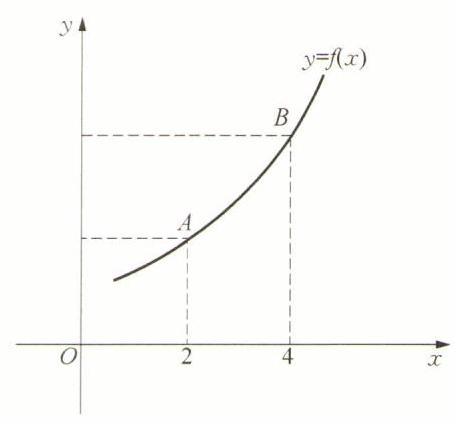
\includegraphics[width=0.3\textwidth]{bodyxb/src/bo_d1ig044601uc738hj6v0_117_1039_1019_455_422_0.jpg}
\end{center}

第 1 题图

A. ${f}^{\prime }\left( 2\right)  < \dfrac{f\left( 4\right)  - f\left( 2\right) }{2} < {f}^{\prime }\left( 4\right)$

B. ${f}^{\prime }\left( 4\right)  < {f}^{\prime }\left( 2\right)  < \dfrac{f\left( 4\right)  - f\left( 2\right) }{2}$

C. ${f}^{\prime }\left( 2\right)  < {f}^{\prime }\left( 4\right)  < \dfrac{f\left( 4\right)  - f\left( 2\right) }{2}$

D. $\dfrac{f\left( 4\right)  - f\left( 2\right) }{2} < {f}^{\prime }\left( 4\right)  < {f}^{\prime }\left( 2\right)$

2. 已知 $f\left( x\right)$ 是定义在 ${R}$ 上的可导函数,若 $\mathop{\lim }\limits_{{{\Delta x} \rightarrow  0}}\dfrac{f\left( 2\right)  - f\left( {2 + {\Delta x}}\right) }{2\Delta x} = \dfrac{1}{2}$ ,则 ${f}^{\prime }\left( 2\right)  =$ (   ).

A. -1 B. $- \dfrac{1}{4}$ C. 1 D. $\dfrac{1}{4}$

3. 设函数 $f\left( x\right)$ 的导函数为 ${f}^{\prime }\left( x\right)$ ,且 $f\left( x\right)  = \cos x - {f}^{\prime }\left( \dfrac{\pi }{6}\right) x$ ,则 $f\left( \dfrac{\pi }{2}\right)  =$ \blkda{}.

4. 求下列函数的导数:

(1) $y = \left( {3{x}^{2} + {2x} + 1}\right) \cos x$ ; (2) $y = \dfrac{3{x}^{2} + x\sqrt{x} - 5\sqrt{x} + 1}{\sqrt{x}}$ ;

(3) $y = {2}^{x}\cos x - {3x}{\log }_{3}x$ ; (4) $y = \sqrt[3]{\cos \left( {{2}^{x} + x}\right) }$ ;

(5) $y = {\cos }^{2}\left( \dfrac{1 + {x}^{2}}{{{e}}^{x}}\right)$ .

5. 已知函数 $f\left( x\right)  = {{e}}^{x} - x,g\left( x\right)  = {x}^{2} - x$ ,令 $u\left( x\right)  = f\left( {g\left( x\right) }\right) ,v\left( x\right)  = g\left( {f\left( x\right) }\right)$ ,则 (   ).

A. $u\left( x\right)$ 与 $g\left( x\right)$ 的单调区间相同 B. $v\left( x\right)$ 与 $f\left( x\right)$ 的单调区间相同

C. $u\left( x\right)$ 与 $f\left( x\right)$ 有相同的最小值 D. $v\left( x\right)$ 与 $g\left( x\right)$ 有相同的最小值

\subsection*{56 切线}

\subsubsection*{知识点睛}

求切线方程, 确定切点的坐标, 根据切线求参数的值和范围一直是高考的热点.

求切线的步骤为:设切点 $P\left( {{x}_{0},f\left( {x}_{0}\right) }\right)$ ；求切线斜率 $k = {f}^{\prime }\left( {x}_{0}\right)$ ；写切线方程 $y - f\left( {x}_{0}\right)  =$  ${f}^{\prime }\left( {x}_{0}\right) \left( {x - {x}_{0}}\right)$ ,最后化简.

特别要注意,求切线时看清楚是求在某点处的切线还是过某点的切线.

\subsubsection*{经典习题}

1. 曲线 $y = \ln \left| x\right|$ 过坐标原点的两条切线的方程为\blkda{},\blkda{}.

2. 若曲线 $y = \left( {{2x} - a}\right) {{e}}^{x}$ 有两条过坐标原点的切线,则实数 $a$ 的取值范围为\blkda{}.

3. 已知直线 $y = x + 1$ 与曲线 $y = \ln \left( {x + a}\right)$ 相切,则 $a$ 的值为\blkda{}.

4. 已知函数 $f\left( x\right)  = \left| {{{e}}^{x} - 1}\right| ,{x}_{1} < 0,{x}_{2} > 0$ ,函数 $f\left( x\right)$ 的图象在点 $A\left( {{x}_{1},f\left( {x}_{1}\right) }\right)$ 和点 $B\left( {{x}_{2},f\left( {x}_{2}\right) }\right)$ 的两条切线互相垂直,且分别交 $y$ 轴于 $M,N$ 两点,则 $\dfrac{\left| AM\right| }{\left| BN\right| }$ 的取值范围是\blkda{}.

5. 设函数 $f\left( x\right)  = \dfrac{1}{2}{x}^{2} + {2ax}\left( {a > 0}\right)$ 的图象与 $g\left( x\right)  = 3{a}^{2}\ln x + b$ 的图象有公共点,且在公共点处的切线重合,则实数 $b$ 的最大值为\blkda{}.

6. 若过点(1, a)可以作出曲线 $y = \left( {x - 1}\right) {{e}}^{x}$ 的切线 $l$ ,且 $l$ 最多有 $n$ 条, $n \in  {\mathbf{N}}^{ * }$ ,则(   ). A. $a \leq  0$

B. 当 $n = 2$ 时, $a$ 值唯一

C. 当 $n = 1$ 时, $a <  - \dfrac{4}{{e}}$

D. ${na}$ 的值可以取到 -4

7. 若两曲线 $y = \ln x - 1$ 与 $y = a{x}^{2}$ 存在公切线,则正实数 $a$ 的取值范围是\blkda{}.

8. 已知函数 $f\left( x\right)  = 2\ln x,g\left( x\right)  = a{x}^{2} - x - \dfrac{1}{2}\left( {a > 0}\right)$ ,若直线 $y = {2x} - b$ 与函数 $y = f\left( x\right)$ , $y = g\left( x\right)$ 的图象均相切,则 $a$ 的值为\blkda{}；若总存在直线与函数 $y = f\left( x\right) ,y = g\left( x\right)$ 图象均相切,则 $a$ 的取值范围是\blkda{}.

9. 若曲线 ${C}_{1} : y = a{x}^{2}$ 与曲线 ${C}_{2} : y = {{e}}^{x}$ (其中无理数 ${e} = {2.718}\cdots$ ) 存在公切线,则整数 $a$ 的最值情况为(   ).

A. 最大值为 2 , 没有最小值 B. 最小值为 2 , 没有最大值

C. 既没有最大值也没有最小值 D. 最小值为 1 , 最大值为 2

\subsection*{57 切线的应用}

\subsubsection*{知识点睛}

切线的考法非常灵活,应用非常广泛. 考试中经常通过切线问题来研究最值,交点个数问题等. 解决此类问题的关键就是对模型的转化.

\subsubsection*{经典习题}

1. 点 $P$ 是曲线 $y = {x}^{2} - \ln x$ 上的任意一点,则点 $P$ 到直线 $y = x - 2$ 的最小距离为\blkda{}.

2. 若实数 $a,b,c,d$ 满足 $b = {a}^{2} - \ln a,d = c - 2$ ,则 ${\left( a - c\right) }^{2} + {\left( b - d\right) }^{2}$ 的最小值是\blkda{}.

3. 若 $\dfrac{{x}_{1}\left( {\ln {x}_{1} - 1}\right) }{{y}_{1}} = \dfrac{2\left( {{x}_{2} - 5}\right) }{{y}_{2}} = 1$ ,则 ${\left( {x}_{1} - {x}_{2}\right) }^{2} + {\left( {y}_{1} - {y}_{2}\right) }^{2}$ 的最小值为 (   ).

A. $\dfrac{{10}\sqrt{5} - \sqrt{5}{{e}}^{2}}{5}$ B. $\dfrac{{10}\sqrt{5} + \sqrt{5}{{e}}^{2}}{5}$

C. $\dfrac{{{e}}^{4} - {20}{{e}}^{2} + {100}}{5}$ D. $\dfrac{5}{4}{{e}}^{4} + 5{{e}}^{2} + 5$

4. 已知 $P$ 为直线 $x + {2y} - 1 = 0$ 上的一个动点, $Q$ 为曲线 $4{x}^{4} - 2{x}^{2}y - {x}^{3} + 2{x}^{2} + 1 = 0$ 上的一个动点,则线段 ${PQ}$ 长度的最小值为\blkda{}.

5. 对任意实数 $a,b,{{e}}^{2a} - {2b}\left( {{{e}}^{a} + a}\right)  + {a}^{2} + 2{b}^{2}$ 的最小值是 (   ).

A. $\dfrac{1}{4}$ B. $\dfrac{1}{2}$ C. $\dfrac{3}{4}$ D. 1

6. 已知函数 $f\left( x\right)  = {{e}}^{x} + {x}^{2} + \ln x$ 与函数 $g\left( x\right)  = {{e}}^{-x} + 2{x}^{2} - {ax}$ 的图象上存在关于 $y$ 轴对称的点,则实数 $a$ 的取值范围为(   ).

A. $( - \infty , - {e}\rbrack$ B. $( - \infty , - 1\rbrack$ C. $( - \infty , - \dfrac{1}{2}\rbrack$ D. $\left( {-\infty , - \dfrac{1}{{e}}}\right\rbrack$

7. 若存在实常数 $k$ 和 $b$ ,使得函数 $F\left( x\right)$ 和 $G\left( x\right)$ 对其公共定义域上的任意实数 $x$ 都满足: $F\left( x\right)  \geq  {kx} + b$ 和 $G\left( x\right)  \leq  {kx} + b$ 恒成立,则称此直线 $y = {kx} + b$ 为 $F\left( x\right)$ 和 $G\left( x\right)$ 的“隔离直线”,已知函数 $f\left( x\right)  = {x}^{2}\left( {x \in  \mathbf{R}}\right) ,g\left( x\right)  = \dfrac{1}{x}\left( {x < 0}\right) ,h\left( x\right)  = 2\operatorname{eln}x\left( {x > 0}\right)$ ,有下列两个命题:

命题 $\alpha  : f\left( x\right)$ 和 $h\left( x\right)$ 之间存在唯一的“隔离直线” $y = 2\sqrt{{e}}x - {e}$ ；

命题 $\beta  : f\left( x\right)$ 和 $g\left( x\right)$ 之间存在“隔离直线”,且 $b$ 的最小值为 -1.

则下列说法正确的是(   ).

A. 命题 $\alpha$ 、命题 $\beta$ 都是真命题

B. 命题 $\alpha$ 为真命题,命题 $\beta$ 是假命题

C. 命题 $\alpha$ 为假命题,命题 $\beta$ 是真命题

D. 命题 $\alpha$ 、命题 $\beta$ 都是假命题

\subsection*{58 导数与单调性}

\subsubsection*{知识点睛}

1. 在某个区间(a, b)内,如果 ${f}^{\prime }\left( x\right)  \geq  0$ 恒成立,那么函数 $y = f\left( x\right)$ 在这个区间内单调递增; 如果 ${f}^{\prime }\left( x\right)  \leq  0$ ,那么函数 $y = f\left( x\right)$ 在这个区间内单调递减.

2. 已知函数单调性, 求参数范围的两个方法:

① 利用集合间的包含关系处理: $y = f\left( x\right)$ 在(a, b)上单调,则区间(a, b)是相应单调区间的子集.

② 转化为不等式的恒成立问题来求解:即“若函数单调递增,则 ${f}^{\prime }\left( x\right)  \geq  0$ ；若函数单调递减,则 ${f}^{\prime }\left( x\right)  \leq  {0}^{\prime \prime }$ .

3. 若可导函数 $f\left( x\right)$ 在指定的区间 $D$ 上严格单调递增 (减),求参数范围问题,可转化为 ${f}^{\prime }\left( x\right)  \geq  0$ [或 ${f}^{\prime }\left( x\right)  \leq  0$ ]恒成立问题,从而构建不等式,要注意 “ $=$ ” 不能省略,否则可能会漏解.

\begin{center}
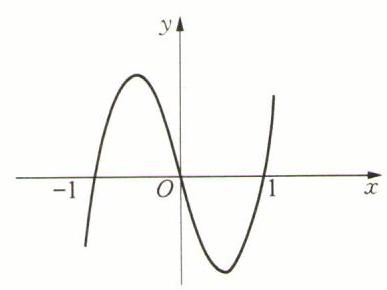
\includegraphics[width=0.3\textwidth]{bodyxb/src/bo_d1ig044601uc738hj6v0_123_1093_1199_387_290_0.jpg}
\end{center}

第 1 题图

\subsubsection*{经典习题}

1. 已知函数 $y = x{f}^{\prime }\left( x\right)$ 的图象如图所示 (其中 ${f}^{\prime }\left( x\right)$ 是函数 $f\left( x\right)$ 的导函数),则下面四个图象中, $y = f\left( x\right)$ 的图象大致是 (   ).

\begin{center}
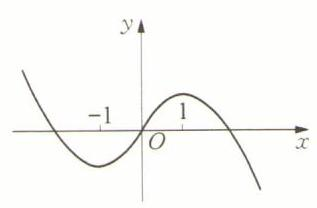
\includegraphics[width=0.2\textwidth]{bodyxb/src/bo_d1ig044601uc738hj6v0_123_131_1565_317_208_0.jpg}
\end{center}

A

\begin{center}
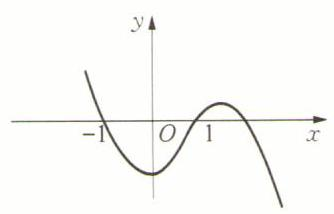
\includegraphics[width=0.2\textwidth]{bodyxb/src/bo_d1ig044601uc738hj6v0_123_465_1556_334_214_0.jpg}
\end{center}

B

\begin{center}
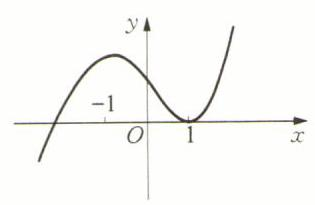
\includegraphics[width=0.2\textwidth]{bodyxb/src/bo_d1ig044601uc738hj6v0_123_814_1562_315_205_0.jpg}
\end{center}

C

\begin{center}
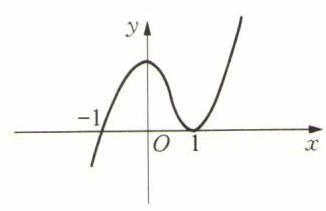
\includegraphics[width=0.2\textwidth]{bodyxb/src/bo_d1ig044601uc738hj6v0_123_1143_1555_326_211_0.jpg}
\end{center}

D

2. 设 $y = {f}^{\prime }\left( x\right)$ 是函数 $y = f\left( x\right)$ 的导函数, $y = f\left( x\right)$ 的图象如图所示,则 $f\left( x\right)  \cdot  {f}^{\prime }\left( x\right)  > 0$ 的解集是 (   ).

\begin{center}
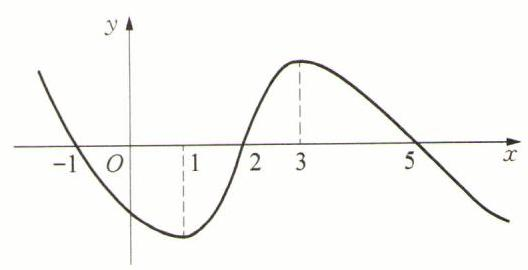
\includegraphics[width=0.4\textwidth]{bodyxb/src/bo_d1ig044601uc738hj6v0_123_958_1823_528_270_0.jpg}
\end{center}

第 2 题图

A. $\left( {2,3}\right)  \cup  \left( {5, + \infty }\right)$

B. $\left( {-\infty ,0}\right)  \cup  \left( {1,3}\right)$

C. $\left( {-1,1}\right)  \cup  \left( {2,3}\right)  \cup  \left( {5, + \infty }\right)$

D. $\left( {-\infty , - 1}\right)  \cup  \left( {1,2}\right)  \cup  \left( {3,5}\right)$

3. 已知 $f\left( x\right)  = 2{x}^{2} - {ax} + \ln x$ 在区间 $\left( {1, + \infty }\right)$ 上单调递增,则实数 $a$ 的取值范围是\blkda{}.

4. 已知函数 $f\left( x\right)  = a\ln \left( {x + 1}\right)  + {x}^{2}$ ,在区间 (3,4) 内任取两个实数 ${x}_{1},{x}_{2}$ 且 ${x}_{1} \neq  {x}_{2}$ ,若不等式 $\dfrac{f\left( {{x}_{1} - 1}\right)  - f\left( {{x}_{2} - 1}\right) }{{x}_{1} - {x}_{2}} > 1$ 恒成立,则实数 $a$ 的取值范围为 (   ).

A. $\lbrack  - 9, + \infty )$ B. $\lbrack  - 7, + \infty )$ C. $\lbrack 9, + \infty )$ D. $\lbrack 7, + \infty )$

5. 任意 ${x}_{1},{x}_{2} \in  \left\lbrack  {1,{e}}\right\rbrack  \left( {{x}_{1} \neq  {x}_{2}}\right)$ ,均有 $\dfrac{{x}_{1}\ln {x}_{2} - {x}_{2}\ln {x}_{1}}{{x}_{2} - {x}_{1}} < a$ 成立,则 $a$ 的取值范围为 (   ).

A. $( - \infty ,1\rbrack$ B. $\lbrack 1, + \infty )$ C. $\left\lbrack  {0,1}\right\rbrack$ D. $\lbrack 0, + \infty )$

6. 已知定义在 $\mathbf{R}$ 上的函数 $f\left( x\right)$ ,其导函数为 ${f}^{\prime }\left( x\right)$ ,若 $f\left( x\right)  - f\left( {-x}\right)  + 2{x}^{3} + {2x} = 0$ ,且当 $x \geq  0$ 时, ${f}^{\prime }\left( x\right)  + 3{x}^{2} + 1 < 0$ ,则不等式 $f\left( {x + 1}\right)  - f\left( x\right)  + 3{x}^{2} + {3x} + 2 \leq  0$ 的解集为 (   ).

A. $( - \infty ,0\rbrack$ B. $\lbrack 0, + \infty )$ C. $( - \infty , - \dfrac{1}{2}\rbrack$ D. $\left\lbrack  {-\dfrac{1}{2}, + \infty }\right)$

7. 已知定义在 $\mathbf{R}$ 上的函数 $f\left( x\right)$ 的导函数为 ${f}^{\prime }\left( x\right)$ ,且 ${3f}\left( x\right)  + {f}^{\prime }\left( x\right)  < 0,f\left( {\ln 2}\right)  = 1$ ,则不等式 $f\left( x\right) {{e}}^{3x} > 8$ 的解集为 (   ).

A. $\left( {-\infty ,2}\right)$ B. $\left( {-\infty ,\ln 2}\right)$ C. $\left( {\ln 2, + \infty }\right)$ D. $\left( {2, + \infty }\right)$

8. 已知定义在 $\left( {-\infty ,0}\right)  \cup  \left( {0, + \infty }\right)$ 上的奇函数 $y = f\left( x\right)$ 的导函数为 $y = {f}^{\prime }\left( x\right)$ ,当 $x >$ 0时, $x{f}^{\prime }\left( x\right)  <  - f\left( x\right)$ ,且 $f\left( 2\right)  = 3$ ,则不等式 ${2xf}\left( {{2x} + 1}\right)  < 6 - f\left( {{2x} + 1}\right)$ 的解集为 (   ).

A. $\left( {-\dfrac{3}{2},\dfrac{1}{2}}\right)$ B. $\left( {-\infty ,\dfrac{1}{2}}\right)$

C. $\left( {-\infty , - \dfrac{3}{2}}\right)  \cup  \left( {\dfrac{1}{2}, + \infty }\right)$ D. $\left( {-\dfrac{3}{2}, - \dfrac{1}{2}}\right)  \cup  \left( {-\dfrac{1}{2},\dfrac{1}{2}}\right)$

9. 已知 ${f}^{\prime }\left( x\right)$ 是定义在 $\mathbf{R}$ 上的函数 $f\left( x\right)$ 的导函数,且 ${f}^{\prime }\left( x\right)  = f\left( x\right)  + \left( {x + 1}\right) {{e}}^{2x},f\left( 0\right)  = 0$ , 若对任意的实数 $x$ ,都有 $f\left( x\right)  \geq  m$ 成立,则实数 $m$ 的最大值为\blkda{}.

10. 若曲线 $f\left( x\right)  = a\ln x + \left( {a + 1}\right) {x}^{2} + 1\left( {a \in  \mathbf{R}}\right)$ 在点 $\left( {1,f\left( 1\right) }\right)$ 处的切线与直线 ${7x} + y -$  $2 = 0$ 平行,且对任意的 ${x}_{1},{x}_{2} \in  \left( {0, + \infty }\right) ,{x}_{1} \neq  {x}_{2}$ ,不等式 $\left| {f\left( {x}_{1}\right)  - f\left( {x}_{2}\right) }\right|  >$  $m\left| {{x}_{1} - {x}_{2}}\right|$ 恒成立,则实数 $m$ 的最大值为 (   ).

A. $\sqrt{3}$ B. $2\sqrt{3}$ C. $4\sqrt{3}$ D. $5\sqrt{3}$

\subsection*{59 利用导数研究图象}

\subsubsection*{知识点睛}

函数题大多数都是研究函数走势(单调性)和极值(最值),而导数作为一个重要工具,通过计算导数的正负和极限值及极值可以作出函数的草图,作出草图后大多数函数问题也就迎刃而解了.

\subsubsection*{经典习题}

1. 已知关于 $x$ 的方程 ${x}^{2} - \dfrac{1}{{{e}}^{ax}} = 0$ 有唯一实数根,则实数 $a$ 的取值范围为\blkda{}.

2. 已知点 $P$ 是曲线 $y = \sin x + \ln x$ 上任意一点,记直线 ${OP}$ ( $O$ 为坐标原点) 的斜率为 $k$ ,则使得 $k =  - 1$ 的点 $P$ 的个数为(   ).

A. 0 B. 仅有 1 个

C. 仅有 2 个 D. 至少有 3 个

3. 若过点 $P\left( {1,m}\right) \left( {m \in  \mathbf{R}}\right)$ 有 3 条直线与函数 $f\left( x\right)  = x{{e}}^{x}$ 的图象相切,则 $m$ 的取值范围是\blkda{}.

4. 函数 $f\left( x\right) ,g\left( x\right)$ 的定义域都是 $D$ ,直线 $x = {x}_{0}\left( {{x}_{0} \in  D}\right)$ 与 $y = f\left( x\right) ,y = g\left( x\right)$ 的图象分别交于 $A,B$ 两点,若线段 ${AB}$ 的长度是不为 0 的常数,则称曲线 $y = f\left( x\right) ,y = g\left( x\right)$ 为 “平行曲线”. 设 $f\left( x\right)  = {{e}}^{x} - a\ln x + c\left( {a > 0,c \neq  0}\right)$ ,且 $y = f\left( x\right) ,y = g\left( x\right)$ 为区间 $(0$ , $+ \infty )$ 的“平行曲线”,其中 $g\left( 1\right)  = {e},g\left( x\right)$ 在区间(2,3)上的零点唯一,则 $a$ 的取值范围是 (   ).

A. $\left( {\dfrac{{{e}}^{2}}{\ln 3},\dfrac{{{e}}^{4}}{\ln 2}}\right)$ B. $\left( {\dfrac{{{e}}^{2}}{\ln 2},\dfrac{{{e}}^{3}}{\ln 3}}\right)$

C. $\left( {\dfrac{{{e}}^{3}}{\ln 3},\dfrac{2{{e}}^{4}}{\ln 2}}\right)$ D. $\left( {\dfrac{2{{e}}^{3}}{\ln 3},\dfrac{{{e}}^{4}}{\ln 2}}\right)$

5. 已知函数 $f\left( x\right)$ 的导函数为 ${f}^{\prime }\left( x\right)$ ,且对任意的实数 $x$ 都有 ${f}^{\prime }\left( x\right)  = {{e}}^{-x}\left( {{2x} + \dfrac{5}{2}}\right)  -$  $f\left( x\right)$ (e 是自然对数的底数),且 $f\left( 0\right)  = 1$ ,若关于 $x$ 的不等式 $f\left( x\right)  - m < 0$ 的解集中恰有唯一一个整数,则实数 $m$ 的取值范围是 (   ).

A. $\left( {-\dfrac{{e}}{2},0}\right)$ B. $\left( {-\dfrac{{e}}{2},0}\right\rbrack$ C. $\left( {-\dfrac{3{e}}{4},0}\right\rbrack$ D. $\left( {-\dfrac{3{e}}{4},\dfrac{9}{2{e}}}\right\rbrack$

6. 已知函数 $f\left( x\right)  = 4\operatorname{eln}x - \dfrac{{x}^{2}}{x - \operatorname{eln}x} + {mx}$ 存在 4 个零点,则实数 $m$ 的取值范围是\blkda{}.

7. 已知函数 $f\left( x\right)  = \sin {ax} - a\sin x$ 在 $\left( {0,{2\pi }}\right)$ 上有零点,则实数 $a$ 的取值范围是\blkda{}.

\subsection*{60 导数与极值}

\subsubsection*{知识点睛}

理解极值的定义, 对于可导函数, 知道极值点与驻点的区别. 极大值点为 “前增后减” 的点, 即导函数“前正后负”的零点. 极小值点为“前减后增”的点,即导函数“前负后正”的零点.

另外极值点的导数不一定为 0 ,极值点不能是端点.

求极值点的常见步骤为:先求导(若函数可导),再求出驻点. 然后列表研究导数在各个区间的正负, 最后判别各个驻点是否是极值点.

\subsubsection*{经典习题}

1. 已知函数 $y = f\left( x\right) \left( {a < x < b}\right)$ 的导函数是 $y = {f}^{\prime }\left( x\right)$  $\left( {a < x < b}\right)$ ,导函数 $y = {f}^{\prime }\left( x\right)$ 的图象如图所示,则函数 $y = f\left( x\right)$ 在(a, b)内有(   ).

\begin{center}
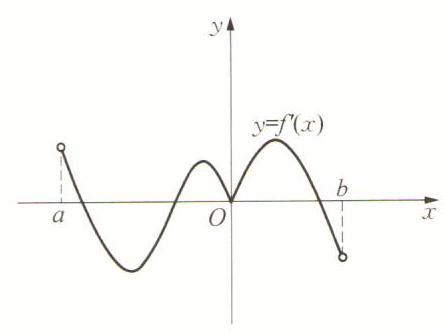
\includegraphics[width=0.3\textwidth]{bodyxb/src/bo_d1ig044601uc738hj6v0_127_1037_1028_443_332_0.jpg}
\end{center}

第 1 题图

A. 3 个驻点

B. 4 个极值点

C. 1 个极小值点

D. 1 个极大值点

2. 函数 $f\left( x\right)  = {x}^{3} - a{x}^{2} - {bx} + {a}^{2}$ 在 $x = 1$ 处有极值 10,则点(a, b)为(   ).

A.(3, - 3) B.(-4,11)

C.(3, - 3)或(-4,11) D.(4,11)

3. 设 $a \neq  0$ ,若 $x = a$ 为函数 $f\left( x\right)  = a{\left( x - a\right) }^{2}\left( {x - b}\right)$ 的极大值点,则(   ).

A. $a < b$ B. $a > b$

C. ${ab} < {a}^{2}$ D. ${ab} > {a}^{2}$

4. 已知函数 $f\left( x\right)  = \cos x + \left( {a - 1}\right) {{e}}^{x}$ 在 $\left( {-\pi ,\pi }\right)$ 上恰有一个极值,则 $a =$ \blkda{}.

5. 已知函数 $f\left( x\right)  = {x}^{3} - 3{x}^{2} - {9x} + {14}$ ,若函数 $F\left( x\right)  = \left| {f\left( x\right)  - a}\right|$ 恰好有两个极大值点, 则常数 $a$ 的取值范围是\blkda{}.

6. 若函数 $f\left( x\right)  = \dfrac{{{e}}^{x}}{{x}^{3}} - a\left( {\dfrac{3}{x} + \ln x}\right)$ 只有一个极值点,则 $a$ 的取值范围是\blkda{}.

7. 已知 $x = {x}_{1}$ 和 $x = {x}_{2}$ 分别是函数 $f\left( x\right)  = 2{a}^{x} - {e}{x}^{2}\left( {a > 0\text{ 且 }a \neq  1}\right)$ 的极小值点和极大值点. 若 ${x}_{1} < {x}_{2}$ ,则 $a$ 的取值范围是\blkda{}.

8. 设函数 $f\left( x\right)$ 满足 ${x}^{2}{f}^{\prime }\left( x\right)  + {2xf}\left( x\right)  = \dfrac{{{e}}^{x}}{x},f\left( 2\right)  = \dfrac{{{e}}^{2}}{8}$ ,则 $x > 0$ 时, $f\left( x\right)$ (   ).

A. 有极大值, 无极小值 B. 有极小值, 无极大值

C. 既有极大值又有极小值 D. 既无极大值也无极小值

9. 已知函数 $f\left( x\right)  = {{e}}^{2x} - {{e}}^{-{2x}} - {ax}$ ,若 $f\left( x\right)$ 有两个不同的极值点 ${x}_{1},{x}_{2}$ ,且 $0 < {x}_{2} - {x}_{1} <$  $\ln 2$ ,则 $a$ 的取值范围为\blkda{}.

10. 已知曲线 $y = \dfrac{x}{{{e}}^{x}}$ 在 $x = {x}_{1}$ 处的切线为 ${l}_{1}$ ,曲线 $y = \ln x$ 在 $x = {x}_{2}$ 处的切线为 ${l}_{2}$ ,且 ${l}_{1}\bot {l}_{2}$ , 则 ${x}_{2} - {x}_{1}$ 的取值范围是 (   ).

A. $\left( {0,\dfrac{1}{{e}}}\right)$ B. $\left( {-\infty , - 1}\right)$ C. $\left( {-\infty ,0}\right)$ D. $\left( {-\infty ,\dfrac{1}{{e}}}\right)$

11. 关于函数 $f\left( x\right)  = \dfrac{2}{x} + \ln x$ ,下列判断正确的是 (   ).

① $x = 2$ 是 $f\left( x\right)$ 的极大值点;

② 函数 $y = f\left( x\right)  - x$ 有且只有 1 个零点;

③ 存在正实数 $k$ ,使得 $f\left( x\right)  > {kx}$ 成立；

④ 对任意两个正实数 ${x}_{1},{x}_{2}$ ,且 ${x}_{1} > {x}_{2}$ ,若 $f\left( {x}_{1}\right)  = f\left( {x}_{2}\right)$ ,则 ${x}_{1} + {x}_{2} > 4$ .

A. ①④ B. ②③ C. ②④ D. ①③

\subsection*{61 有解恒成立问题}

\subsubsection*{知识点睛}

有解、恒成立问题一直是函数考察的重点. 解决此类问题主要有参变分离、数形结合、整体求最值、构造单调函数等方法. 具体处理方式大家可以通过以下习题领悟.

\subsubsection*{经典习题}

1. 设函数 $f\left( x\right)  = \left( {x - 1}\right) \left( {{{e}}^{x} - {e}}\right) ,g\left( x\right)  = {{e}}^{x} - {ax} - 1$ ,其中 $a \in  \mathbf{R}$ . 若对任意 ${x}_{2} \in  \lbrack 0$ , $+ \infty$ ),都存在 ${x}_{1} \in  \mathbf{R}$ ,使得不等式 $f\left( {x}_{1}\right)  \leq  g\left( {x}_{2}\right)$ 成立,则 $a$ 的最大值为 (   ).

A. 0 B. $\dfrac{1}{{e}}$ C. 1 D. ${e}$

2. 已知函数 $f\left( x\right)  = {{e}}^{x} - x\ln x + {x}^{2},g\left( x\right)  =  - {x}^{3} + 2{x}^{2} + {ax}$ ,若关于 $x$ 的不等式 $f\left( x\right)  \leq$  $g\left( x\right)$ 有解,则实数 $a$ 的取值范围为\blkda{}.

3. 已知 $f\left( x\right)  = {{e}}^{2x} + {{e}}^{x + 2} - 2{{e}}^{4},g\left( x\right)  = {x}^{2} - {3a}{{e}}^{x},A = \{ x \mid  f\left( x\right)  = 0\} ,B = \{ x \mid  g\left( x\right)  =$  $0\}$ ,若存在 ${x}_{1} \in  A,{x}_{2} \in  B$ ,使得 $\left| {{x}_{1} - {x}_{2}}\right|  < 1$ ,则实数 $a$ 的取值范围为\blkda{}.

4. 若关于 $x$ 的不等式 $x{{e}}^{x} - a\left( {x + 3}\right)  - a\ln x \geq  0$ 恒成立,则实数 $a$ 的取值范围是\blkda{}.

5. 已知不等式 $a{{e}}^{x}\left( {x + 3}\right)  - x - 2 < 0\left( {a < 1}\right)$ 恰有 2 个整数解,则 $a$ 的取值范围为 (   ). A. $\dfrac{3}{4{{e}}^{2}} \leq  a < \dfrac{2}{3{e}}$ B. $\dfrac{3}{4{{e}}^{2}} < a \leq  \dfrac{2}{3{e}}$ C. $\dfrac{3}{4{e}} \leq  a < \dfrac{2}{3}$ D. $\dfrac{3}{4{e}} < a \leq  \dfrac{2}{3}$

6. 对任意 $k \geq  1$ ,存在 $x \in  \left\lbrack  {2,4}\right\rbrack$ ,使不等式 $\left( {{x}^{k} + x + k\ln x}\right)  \cdot  {{e}}^{x} \geq  a{{e}}^{x} + {{e}}^{a}$ 成立,则实数 $a$ 的取值范围是\blkda{}.

7. 若函数 $f\left( x\right)  = {{e}}^{ax} - \dfrac{\ln x}{a}\left( {a > 0}\right)$ 存在零点,则 $a$ 的取值范围是 (   ).

A. $\left( {0,\dfrac{1}{{e}}}\right\rbrack$ B. $\left( {0,\dfrac{1}{{{e}}^{2}}}\right\rbrack$ C. $\left\lbrack  {\dfrac{1}{{{e}}^{2}},\dfrac{1}{{e}}}\right\rbrack$ D. $\left\lbrack  {\dfrac{1}{{e}}, + \infty }\right)$

8. 若 ${{e}}^{x + 1} - \dfrac{\ln x + {2k}}{x} - k \geq  0$ 对任意 $x > 0$ 恒成立,则实数 $k$ 的取值范围是\blkda{}.

9. 若 ${2x} + 8{x}^{3} + {a}^{2}{{e}}^{2x} < 4{x}^{2} + a{{e}}^{x} + {a}^{3}{{e}}^{3x}$ 对 $x \in  \mathbf{R}$ 恒成立,则 $a$ 的取值范围是\blkda{}.

62 导数的实际应用

\subsubsection*{知识点睛}

在实际应用过程中, 我们过往经常会建立数学模型, 求出目标函数. 但因为目标函数比较复杂甚至为超越函数而得不到我们想要的结果. 现在我们则可以利用导数工具, 快速得到我们想要的结果.

\subsubsection*{经典习题}

1. 已知某商品的成本 $C$ 和产量 $q$ 满足关系 $C = {50000} + {200q}$ ,该商品的销售单价 $p$ 和产量 $q$ 满足关系式 $p = {24200} - \dfrac{1}{5}{q}^{2}$ ,则当产量 $q$ 等于\blkda{}时,利润最大.

2. 已知正四棱锥的侧棱长为 $l$ ,其各顶点都在同一球面上. 若该球的体积为 ${36\pi }$ ,且 $3 \leq  l \leq$  $3\sqrt{3}$ ,则该正四棱锥体积的取值范围是 (   ).

A. $\left\lbrack  {{18},\dfrac{81}{4}}\right\rbrack$ B. $\left\lbrack  {\dfrac{27}{4},\dfrac{81}{4}}\right\rbrack$ C. $\left\lbrack  {\dfrac{27}{4},\dfrac{64}{3}}\right\rbrack$ D. $\left\lbrack  {{18},{27}}\right\rbrack$

3. 已知抛物线 ${x}^{2} = {3y}$ ,动点 $A$ 自原点出发,沿着 $y$ 轴正方向向上匀速运动,速度大小为 $v$ . 过 $A$ 作 $y$ 轴的垂线交抛物线于 $B$ 点,再过 $B$ 作 $x$ 轴的垂线交 $x$ 轴于 $C$ 点. 当 $A$ 运动至 ( 0 , 100 )时,点 $C$ 的瞬时速度的大小为\blkda{}.

4. 曲线的曲率就是针对曲线上某个点的切线方向角对弧长的转动率,表明曲线偏离直线的程度, 曲率越大, 表示曲线的弯曲程度越大, 工程规划中常需要计算曲率, 如高铁的弯道设计. 曲线 $y = f\left( x\right)$ 在点 $\left( {x,f\left( x\right) }\right)$ 曲率的计算公式是 $K = \dfrac{\left| {y}^{\prime \prime }\right| }{\sqrt{{\left\lbrack  1 + {\left( {y}^{\prime }\right) }^{2}\right\rbrack  }^{3}}}$ ,其中 ${y}^{\prime \prime }$ 是 ${y}^{\prime }$ 的导函数,则曲线 ${xy} = 1$ 上点的曲率的最大值是\blkda{}.

5. 潮汐现象是地球上的海水在太阳和月球双重引力作用下产生的全球性的海水的周期性变化,人们可以利用潮汐进行港口货运. 某港口具体时刻 $t$ (单位:时) 与对应水深 $y$ (单位:米)的函数关系式为 $y = 3\sin \dfrac{\pi }{6}t + {10}\left( {0 \leq  t \leq  {24}}\right)$ . 某艘大型货船要进港,其相应的吃水深度(船底与水面的距离) 为 7 米, 船底与海底距离不小于 4.5 米时就是安全的, 该船于 2 点开始卸货 (一次卸货最长时间不超过 8 小时),同时吃水深度以 0.375 米/时的速度减少,该船 8 小时内没有卸完货,要及时驶入深水区域,则该船第一次停止卸货的时刻为\blkda{}.

\subsection*{63 导函数的性质}

\subsubsection*{知识点睛}

函数 $f\left( x\right)$ 可导,若函数 $f\left( x\right)$ 关于 $x = a$ 对称,则其导函数 ${f}^{\prime }\left( x\right)$ 必关于点(a,0)对称；若函数 $f\left( x\right)$ 关于点(a, b)对称,则其导函数 ${f}^{\prime }\left( x\right)$ 必关于 $x = a$ 对称;

函数 $f\left( x\right)$ 可导,若函数 ${f}^{\prime }\left( x\right)$ 关于 $x = a$ 对称,则函数 $f\left( x\right)$ 必关于点 $\left( {a,b}\right) \left( {b\text{ 未知)对 }}\right)$ 称；若函数 ${f}^{\prime }\left( x\right)$ 关于点(a,0)对称,则函数 $f\left( x\right)$ 必关于 $x = a$ 对称；

函数 $f\left( x\right)$ 可导,若函数 $f\left( x\right)$ 为周期函数,则其导函数 ${f}^{\prime }\left( x\right)$ 必为周期函数；若 ${f}^{\prime }\left( x\right)$ 为周期函数,其原函数 $f\left( x\right)$ 不一定为周期函数.

\subsubsection*{经典习题}

1. 已知函数 $y = f\left( x\right)$ 及其导函数 $y = {f}^{\prime }\left( x\right)$ 的定义域都是 R. 以下命题是真命题的有\blkda{}.

① 若函数 $y = f\left( x\right)$ 是奇函数,则 $y = {f}^{\prime }\left( x\right)$ 是偶函数；② 若 $y = {f}^{\prime }\left( x\right)$ 是偶函数,则函数 $y = f\left( x\right)$ 是奇函数；③ 若函数 $y = {f}^{\prime }\left( x\right)$ 是周期函数,则 $y = f\left( x\right)$ 也是周期函数；④ 若 $y =$  ${f}^{\prime }\left( x\right)$ 是严格单调递增函数,则函数 $y = f\left( x\right)$ 也是严格单调递增函数.

2. 已知函数 $f\left( x\right)$ 及其导函数 ${f}^{\prime }\left( x\right)$ 的定义域均为 $\mathbf{R}$ 且都为连续函数,记 $g\left( x\right)  = {f}^{\prime }\left( x\right)$ ,若 $f\left( {1 - x}\right) ,g\left( x\right)$ 均为奇函数, $g\left( 1\right)  = 2$ ,则 $f\left( {2023}\right)  + g\left( {2023}\right)  =$ (   ).

A. -2 B. 0

C. 2 D. 2023

3. 已知函数 $f\left( x\right)$ 及其导函数 ${f}^{\prime }\left( x\right)$ 的定义域均为 $\mathbf{R}$ ,记 $g\left( x\right)  = {f}^{\prime }\left( x\right)$ ,若 $f\left( {\dfrac{3}{2} - {2x}}\right)$ , $g\left( {2 + x}\right)$ 均为偶函数,则 (   ).

A. $f\left( 0\right)  = 0$ B. $g\left( {-\dfrac{1}{2}}\right)  = 0$

C. $f\left( {-1}\right)  = f\left( 4\right)$ D. $g\left( {-1}\right)  = g\left( 2\right)$

4. 已知函数 $f\left( x\right)  = {4x} - {x}^{3}$ ,若任意 ${x}_{1},{x}_{2} \in  \left\lbrack  {a,b}\right\rbrack  ,{x}_{1} \neq  {x}_{2}$ ,都有 ${2f}\left( {{x}_{1} + {x}_{2}}\right)  >$  $f\left( {2{x}_{1}}\right)  + f\left( {2{x}_{2}}\right)$ 成立,则满足条件的一个区间是\blkda{}.

5. 已知函数 $f\left( x\right)$ 和 $g\left( x\right)$ 及其导函数 ${f}^{\prime }\left( x\right)$ 和 ${g}^{\prime }\left( x\right)$ 的定义域均为 $\mathbf{R}$ ,若 $f\left( {x + 3}\right)  =$  $g\left( {-x}\right)  + 4,{f}^{\prime }\left( x\right)  + {g}^{\prime }\left( {1 + x}\right)  = 0$ ,且 $g\left( {{2x} + 1}\right)$ 为偶函数,则 (   ) .

A. ${g}^{\prime }\left( 1\right)  = 0$

B. 函数 $f\left( x\right)$ 的图象关于直线 $x = 2$ 对称

C. 函数 ${f}^{\prime }\left( x\right)$ 的图象关于直线 $x = 1$ 对称

D. $\mathop{\sum }\limits_{{k = 1}}^{{2023}}{f}^{\prime }\left( k\right) {g}^{\prime }\left( k\right)  = 1$

\subsection*{64 函数同构}

\subsubsection*{知识点睛}

对于一些函数不等式, 特别是一些双变量的不等式, 直接求解有很大的困难. 这时通过一些同构变换,整理变成 $f\left( {h\left( x\right) }\right)  \sim  f\left( {g\left( x\right) }\right)$ 的形式,或许可以得到意想不到的奇效. 同构在处理指对混合的不等式时尤为好用,例如 ${{e}}^{ax} + {ax} > \ln {x}^{3} + {x}^{3}$ ,我们可以构造 $f\left( x\right)  = {{e}}^{x} + x$ ,转换为 $f\left( {ax}\right)  > f\left( {\ln {x}^{3}}\right)$ ,进而通过研究函数性质 (奇偶性、单调性、对称性、周期性等),得出 ${ax}$ 与 $\ln {x}^{3}$ 的关系,达到简化的目的.

\subsubsection*{经典习题}

1. 若关于 $x$ 的不等式 $\dfrac{x + \ln a}{{{e}}^{x}} > \dfrac{a\ln x}{x}$ 对任意 $x \in  \left( {0,1}\right)$ 恒成立,则实数 $a$ 的取值范围为 (   ).

A. $\left( {-\infty ,\dfrac{1}{{e}}}\right\rbrack$ B. $\left\lbrack  {\dfrac{1}{{e}}, + \infty }\right)$ C. $\left\lbrack  {\dfrac{1}{{e}},1}\right)$ D. $\left( {0,\dfrac{1}{{e}}}\right\rbrack$

2. 已知实数 $a,b$ 满足 $b\left( {{{e}}^{a} - 1}\right)  + a = {{e}}^{b} - \ln b$ ,则 ${b}^{2}{{e}}^{a} - 2{{e}}^{b}$ 的取值范围是\blkda{}.

3. 已知正实数 $x,y$ 满足 $\ln x = y{{e}}^{x} + \ln y$ ,则 $x\left( {y - x + 4}\right)$ 的最大值为\blkda{}.

4. 若对任意的 $0 < {x}_{1} < {x}_{2} \leq  a$ ,都有 ${\left( \dfrac{{x}_{2}}{{x}_{1}}\right) }^{{x}_{1}{x}_{2}} - \dfrac{{{e}}^{e{x}_{2}}}{{{e}}^{e{x}_{1}}} < 0$ 成立,则 $a$ 的最大值为\blkda{}.

5. 若不等式 ${{e}}^{x + a} \geq  \ln x - a$ 恒成立,则实数 $a$ 的取值范围是 (   ).

A. $\lbrack 0, + \infty )$ B. $\lbrack  - 1, + \infty )$

C. $\left\lbrack  {-\dfrac{1}{{e}}, + \infty }\right)$ D. $\lbrack  - {e}, + \infty )$

6. 若对任意 $x \in  \left( {1, + \infty }\right)$ ,不等式 $\left( {\ln a + x - 1}\right) {{e}}^{x - 1} > \dfrac{x}{a}\ln x$ 恒成立,则 $a$ 的取值范围为\blkda{}.

\subsection*{65 导数综合习题}

1. 若函数 $f\left( x\right)  = x\left( {{{e}}^{2x} - a}\right)  - \ln x - 1$ 没有零点,则整数 $a$ 的最大值是 (   ).

A. 3 B. 2 C. 1 D. 0

2. 已知函数 $f\left( x\right)  = {ax} + \ln x + 1 - x{{e}}^{2x}$ 对任意的 $x > 0,f\left( x\right)  \leq  0$ 恒成立,则实数 $a$ 的取值范围为(   ).

A. $( - \infty ,0\rbrack$ B. $( - \infty ,2\rbrack$ C. $( - \infty ,1\rbrack$ D. $( - \infty ,3\rbrack$

3. 已知关于 $x$ 的不等式 $\dfrac{{x}^{4}}{{{e}}^{2x}} - \left( {a + 2}\right) \dfrac{{x}^{2}}{{{e}}^{x}} + {2a} < 0$ 恰有两个正整数解,则实数 $a$ 的取值范围是\blkda{}.

4. 已知函数 $f\left( x\right)  = \dfrac{{{e}}^{x} - {8x}}{m} - x + \dfrac{2{x}^{2}}{{{e}}^{x}}\left( {m \neq  0}\right)$ 有三个零点 ${x}_{1},{x}_{2},{x}_{3}$ ,且有 ${x}_{1} < {x}_{2} < {x}_{3}$ , 则 $\left( {2 - \dfrac{{{e}}^{{x}_{1}}}{{x}_{1}}}\right) \sqrt{\left( {2 - \dfrac{{{e}}^{{x}_{2}}}{{x}_{2}}}\right) \left( {2 - \dfrac{{{e}}^{{x}_{3}}}{{x}_{3}}}\right) }$ 的值为\blkda{}.

5. 已知函数 $f\left( x\right)  = a\sqrt{x - 1} - \ln x + b\left( {a,b \in  \mathbf{R}}\right)$ 在 $\left\lbrack  {{e},{{e}}^{3}}\right\rbrack$ ( ${e}$ 为自然对数的底) 内有零点, 则 ${a}^{2} + {b}^{2}$ 的最小值为\blkda{}.

6. 已知 ${e}$ 为自然对数的底数, $a,b$ 为实数,且不等式 $\ln x + \left( {2{e} - a - 1}\right) x + {2b} + 1 \leq  0$ 对任意的 $x \in  \left( {0, + \infty }\right)$ 恒成立,则 $\dfrac{b + 1}{a + 1}$ 的最大值为\blkda{}.

7. 任意 $a,b \in  \mathbf{R},\dfrac{4\ln x + 3}{4x} \leq  \dfrac{3}{4x} + a + \dfrac{b}{x} \leq  x$ ,则 $b$ 的最大值是\blkda{}.

8. 已知函数 $f\left( x\right)  = \ln x - {ax}$ 有两个零点 ${x}_{1},{x}_{2}\left( {{x}_{1} < {x}_{2}}\right)$ ,则下列说法: ①函数 $f\left( x\right)$ 有极大值点 ${x}_{0}$ ,且 ${x}_{1} + {x}_{2} > 2{x}_{0}$ ；② ${x}_{1}{x}_{2} > {{e}}^{2}$ ；③ ${x}_{1} + 2{x}_{2} > \dfrac{3}{a}$ ； 其中说法正确的有(   ).

A. 0 个 B. 1 个 C. 2 个 D. 3 个

\section*{其他}

这部分我们主要整理了复数、排列组合、概率统计部分的题目.

其实“生活”在二维复平面的复数,比“生活”在一维实数轴上的实数拥有更大的自由度, 会带给我们更广阔的视野. 但是在高中数学的学习中, 我们对复数的要求并不高, 高考试题中考查难度也较小. 所以这里我们仅作少量题目的整理.

相比复数的重要性, 在高中阶段我们很难体会到排列组合与概率统计的重要性. 虽然在高考试题中, 这部分考到填选压轴题的概率较低, 但也不乏一些非常有特色的题目, 会涉及丰富多样的解题方法. 我们整理出来, 帮助同学们在解决问题的过程中培养缜密的数学思维.

\subsection*{66 复数}

\subsubsection*{知识点睛}

1. 复数考点经常与解析几何相联系,看到模长可以从代数的角度转换成几何中距离的概念.

2. 复数问题实数化是最高频使用的方法,即设 $z = a + b{i}\left( {a,b \in  \mathbf{R}}\right)$ .

3. $\left| {z - \left( {a + b{i}}\right) }\right|$ 代表 $z$ 在复平面上所对应的点到(a, b)的距离.

4. 韦达定理在 $\Delta  \geq  0$ 和 $\Delta  < 0$ 时都成立.

5. 设 $a{x}^{2} + {bx} + c = 0\left( {a \neq  0,a,b,c \in  \mathbf{R}}\right)$ 方程两根分别为 ${x}_{1},{x}_{2}$ ,在 $\Delta  < 0$ 时, $\left| {x}_{1}\right|  =$  $\left| {x}_{2}\right|  = \sqrt{\dfrac{c}{a}}.$

6. 设 $a{x}^{2} + {bx} + c = 0\left( {a \neq  0,a,b,c \in  \mathbf{R}}\right)$ 方程两根分别为 ${x}_{1},{x}_{2},\left| {{x}_{1} - {x}_{2}}\right|  = \dfrac{\sqrt{\left| \Delta \right| }}{\left| a\right| }$ .

7. 直接使用求根公式也是解决实系数一元二次方程问题的有力武器.

\subsubsection*{经典习题}

1. 已知复数 ${z}_{1}$ 和 ${z}_{2}$ 满足 $\left| {{z}_{1} - 8 - {14}{i}}\right|  = \sqrt{5}\left| {{z}_{1} - 4 - 6{i}}\right| ,\left| {{z}_{1} - {z}_{2}}\right|  = 3$ ,则 $\left| {\bar{z}}_{2}\right|$ 的取值范围是(   ).

A. $\left\lbrack  {0,{13}}\right\rbrack$ B. $\left\lbrack  {3,9}\right\rbrack$ C. $\left\lbrack  {0,{10}}\right\rbrack$ D. $\left\lbrack  {3,{13}}\right\rbrack$

2. 已知 $z = a + b{i}\left( {a,b \in  \mathbf{R}}\right.$ , ${i}$ 是虚数单位), ${z}_{1},{z}_{2} \in  \mathbf{C}$ ,定义: $D\left( z\right)  = \left| \right| z\left| \right|  = \left| a\right|  + \left| b\right|$ , $D\left( {{z}_{1},{z}_{2}}\right)  = \left| \right| {z}_{1} - {z}_{2}\left| \right|$ ,给出下列命题:

① 对任意 $z \in  \mathbf{C}$ ,都有 $D\left( z\right)  > 0$ ；

② 若 $\bar{z}$ 是 $z$ 的共轭复数,则 $D\left( \bar{z}\right)  = D\left( z\right)$ 恒成立;

③ 若 $D\left( {z}_{1}\right)  = D\left( {z}_{2}\right) \left( {{z}_{1},{z}_{2} \in  \mathbf{C}}\right)$ ,则 ${z}_{1} = {z}_{2}$ ；

④ 对任意 ${z}_{1},{z}_{2},{z}_{3} \in  {C}$ ,则 $D\left( {{z}_{1},{z}_{3}}\right)  \leq  D\left( {{z}_{1},{z}_{2}}\right)  + D\left( {{z}_{2},{z}_{3}}\right)$ 恒成立. 其中真命题是(   ).

A. ①②③④ B. ②③④ C. ②④ D. ②③

3. 已知复数 ${z}_{1}\text{ 、 }{z}_{2}$ 满足 $\left| {{z}_{1} + 1}\right|  + \left| {{z}_{1} - 1}\right|  = 2\sqrt{2},\left| {{z}_{2} - 2{i}}\right|  = 2$ (其中 ${i}$ 是虚数单位),则 $\left| {{z}_{1} - {z}_{2}}\right|$ 的最大值为 (   ).

A. 3 B. 5 C. $2\sqrt{5}$ D. $2\sqrt{2} + 2$

4. 复数 ${z}_{1}\text{ 、 }{z}_{2}$ 满足 $\left| {z}_{2}\right|  = 4,4{z}_{1}^{2} - 2{z}_{1}{z}_{2} + {z}_{2}^{2} = 0$ ,则 $\left| {{\left( {z}_{1} + 1\right) }^{2}\left( {{z}_{1} - 2}\right) }\right|$ 的最大值是\blkda{}.

5. 已知关于 $x$ 的方程: ${x}^{2} - \left( {6 + {i}}\right) x + 9 + a{i} = 0\left( {a \in  \mathbf{R}}\right)$ 有实数根 $b$ ,若复数 $z$ 满足 $\mid  \bar{z} - a -$  $b{i} \mid   = 2\left| z\right|$ ,则 $\left| z\right|$ 的最小值为\blkda{}.

6. 已知集合 $A = \{ x + y{i} \mid  \left| x\right|  \leq  1,\left| y\right|  \leq  1,x,y \in  \mathbf{R}\} ,B = \left\{  {{z}_{2}\left| {{z}_{2} = \left( {\dfrac{3}{4} + \dfrac{3}{4}{i}}\right) {z}_{1}}\right. }\right.$ , ${z}_{1} \in$  $A\}$ ,其中 ${i}$ 为虚数单位,若复数 $z \in  A \cap  B$ ,则 $z$ 对应的点 $Z$ 在复平面内所形成图形的面积为\blkda{}.

7. 设 $m \in  \mathbf{R}$ ,若 $z$ 是关于 $x$ 的方程 ${x}^{2} + {mx} + {m}^{2} - 1 = 0$ 的一个虚根,则 $\left| \bar{z}\right|$ 的取值范围是\blkda{}.

8. 已知 ${x}_{1}$ 与 ${x}_{2}$ 是方程 $a{x}^{2} + {bx} + c = 0\left( {a \neq  0}\right)$ 在复数集中的两根,则下列等式成立的是 (   ).

A. ${x}_{1}$ 与 ${x}_{2}$ 共轭 B. $\Delta  = {b}^{2} - {4ac} \geq  0$

C. ${x}_{1} + {x}_{2} =  - \dfrac{b}{a},{x}_{1}{x}_{2} = \dfrac{c}{a}$ D. $\left| {{x}_{1} - {x}_{2}}\right|  = \sqrt{{\left( {x}_{1} + {x}_{2}\right) }^{2} - 4{x}_{1}{x}_{2}}$

9. 设 $a$ 是实数,关于 $z$ 的方程 $\left( {{z}^{2} - {2z} + 5}\right) \left( {{z}^{2} + {2az} + 1}\right)  = 0$ 有 4 个互不相等的根,它们在复平面上对应的 4 个点共圆,则实数 $a$ 的取值范围是\blkda{}.

10. 实系数一元二次方程 $a{x}^{2} + {bx} + 1 = 0\left( {{ab} \neq  0}\right)$ 有两个虚根 ${z}_{1}\text{ 、 }{z}_{2},{z}_{1}$ 的实部 $\operatorname{Re}\left( {z}_{1}\right)  < 0$ , 且 $\dfrac{{20}^{m} + {21}^{m} - {2020}{z}_{1}}{{29}^{m} - {2020}{z}_{2}}$ 的模等于 1,则实数 $m =$ \blkda{}.

11. 意大利数学家卡尔达诺发明了三次方程的代数解法, 17 世纪人们把卡尔达诺的解法推广, 并整理为四个步骤:

第一步,把方程 ${x}^{3} + {a}_{2}{x}^{2} + {a}_{1}x + {a}_{0} = 0$ 中的 $x$ 用 $x - \dfrac{{a}_{2}}{3}$ 来替换,得到方程 ${x}^{3} + {px} +$  $q = 0;$

第二步,利用公式 ${x}^{3} + {y}^{3} + {z}^{3} - {3xyz} = \left( {x + y + z}\right) \left( {x + {\omega y} + {\omega }^{2}z}\right) \left( {x + {\omega }^{2}y + {\omega z}}\right)$ 将 ${x}^{3} + {px} + q$ 因式分解;

第三步,求得 $y\text{ 、 }z$ 的一组值,得到方程 ${x}^{3} + {px} + q = 0$ 的三个根: $- y - z\text{ 、 } - {\omega y} - {\omega }^{2}z$ 、 $- {\omega }^{2}y - {\omega z}$ (其中 $\omega  = \dfrac{-1 + \sqrt{3}{i}}{2},{i}$ 为虚数单位);

第四步,写出方程 ${x}^{3} + {a}_{2}{x}^{2} + {a}_{1}x + {a}_{0} = 0$ 的根: ${x}_{1} =  - \dfrac{{a}_{2}}{3} - y - z,{x}_{2} =  - \dfrac{{a}_{2}}{3} - {\omega y} - {\omega }^{2}z$ ,

${x}_{3} =  - \dfrac{{a}_{2}}{3} - {\omega }^{2}y - {\omega z}.$

某同学利用上述方法解方程 $8{x}^{3} - {12}{x}^{2} - {42x} + {55} = 0$ 时,得到 $y$ 的一个值: $- 1 + {i}$ ,则下列说法正确的是\blkda{}.

① ${a}_{2} =  - \dfrac{3}{2}$ ; ② ${yz} = 2$ ; ③ ${x}_{2} =  - \dfrac{1}{2} + \sqrt{3}$ ; ④ ${x}_{3} =  - 1 - \sqrt{3}$ .

\subsection*{67 排列组合}

\subsubsection*{知识点睛}

1. 对于排列组合来说, 枚举法与分类讨论一直都是最重要的通法.

2. 不重复选取才是排列组合, 注意你的方法是否会重复选取.

3. 同质化的选取以及整数解相关问题想到隔板法,且要转换为正整数解,而不能是自然数解.

4. 本书中的排列数用 ${{A}}_{n}^{m}$ ,与上海教材中的 ${{P}}_{n}^{m}$ 表达含义一致.

\subsubsection*{经典习题}

1. 把 20 个相同的小球放到三个编号为 1、 2、 3 的盒子里,且每个盒子内的小球数要多于盒子的编号数,则共有\blkda{}种放法.

2. 某组委会要从五名志愿者中选派四人分别从事翻译、导游、礼仪、司机四项不同工作,若其中甲不能从事翻译工作,乙不能从事导游工作,其余三人均能从事这四项工作,则不同的选派方案共有\blkda{}种.

3. 设集合 $A = \left\{  {\left( {{x}_{1},{x}_{2},\cdots ,{x}_{10}}\right)  \mid  {x}_{i} \in  \{  - 1,0,1\} ,i = 1,2,\cdots ,{10}}\right\}$ ,则集合 $A$ 中满足条件 “ $1 \leq  \left| {x}_{1}\right|  + \left| {x}_{2}\right|  + \cdots  + \left| {x}_{10}\right|  \leq  9$ ” 的元素个数为\blkda{}.

4. 设集合 $A = \left\{  {\left( {{x}_{1},{x}_{2},{x}_{3},\cdots ,{x}_{n}}\right)  \mid  {x}_{i} \in  \{  - 1,0,1\} ,i = 1,2,3,\cdots ,n}\right\}$ ,其中 $n \geq  3$ , $n \in  \mathbf{N}$ ,则集合 $A$ 中满足条件 “ $2 \leq  \left| {x}_{1}\right|  + \left| {x}_{2}\right|  + \left| {x}_{3}\right|  + \cdots  + \left| {x}_{n}\right|  \leq  n - 1$ ” 的元素个数为\blkda{}(结果用含有 $n$ 的式子表示).

5. 两名高一年级的学生被允许参加高二年级的学生象棋比赛,每两名参赛选手之间都比赛一次, 胜者得 1 分, 和棋各得 0.5 分, 输者得 0 分, 即每场比赛双方的得分之和是 1 分. 两名高一年级的学生共得 8 分,且每名高二年级的学生都得相同分数,则有\blkda{}名高二年级的学生参加比赛. (结果用数值作答)

6. 在单循环的象棋比赛中 (即每两个人之间比赛一场), 一盘棋中胜者得 1 分, 负者得 0 分, 若平局则各得 0.5 分. 若已知比赛人数至少有 17 人,而最终得分不多于 5 分的人有 11 个,那么得 8.5 分的人有(   )个.

A. 6 B. 5 C. 2 D. 0

7. 用 1、2、3、4、5、6 组成没有重复数字的六位数,要求所有相邻两个数字的奇偶性都不同, 且 1 和 2 相邻,则这样的六位数的个数为(   ).

A. 20 B. 40 C. 60 D. 80

8. ${\left( x + 2y + z\right) }^{11}$ 的展开式为多项式,其展开式经过合并同类项后的项数一共有 (   ).

A. 72 项 B. 75 项 C. 78 项 D. 81 项

9. 从集合 $U = \{ a,b,c,d\}$ 的子集中选出 4 个不同的子集,需同时满足以下两个条件:(1) $\varnothing$ , $U$ 都要选出; (2) 对选出的任意两个子集 $A$ 和 $B$ ,必有 $A \subseteq  B$ 或 $A \supseteq  B$ . 那么,共有\blkda{}种不同的选法.

10. 如图,点 ${P}_{1},{P}_{2},\cdots ,{P}_{10}$ 分别是四面体的顶点或其棱的中点,则在同一平面内的四点组 $\left( {{P}_{1},{P}_{i},{P}_{j},{P}_{k}}\right) \left( {1 < i < j < k \leq  {10}}\right)$ 共有\blkda{}个.

\begin{center}
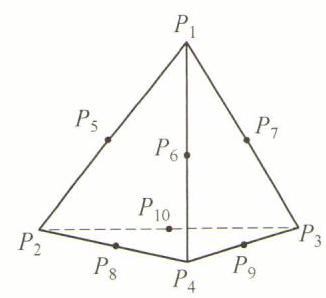
\includegraphics[width=0.2\textwidth]{bodyxb/src/bo_d1ig044601uc738hj6v0_140_1191_590_326_298_0.jpg}
\end{center}

第 10 题图

11. 设 $T$ 是平面直角坐标系 ${xOy}$ 上以 $A\left( {0,2}\right) \text{ 、 }B\left( {-\sqrt{3}, - 1}\right)$ 、 $C\left( {\sqrt{3}, - 1}\right)$ 为顶点的正三角形,考虑一下五种平面上的变换: ① 绕原点作 120° 的逆时针旋转；② 绕原点作 240° 的逆时针旋转； ③关于直线 ${OA}$ 对称；④关于直线 ${OB}$ 对称；⑤关于直线 ${OC}$ 对称. 任选三种变换 (可以相同) 共 125 种变换方式,若要使得 $T$ 变回起始的位置 (即点 $A$ 、 $B\text{ 、 }C$ 分别都在原来的位置),共有 (   ) 种变换方式.

A. 12 B. 16 C. 20 D. 24

12. 定义域为集合 $\{ 1,2,3,\cdots ,{12}\}$ 上的函数 $f\left( x\right)$ 满足:① $f\left( 1\right)  = 1$ ; ② $\left| {f\left( {x + 1}\right)  - f\left( x\right) }\right|  =$  $1\left( {x = 1,2,\cdots ,{11}}\right)$ ；③ $f\left( 1\right)$ 、 $f\left( 6\right)$ 、 $f\left( {12}\right)$ 成等比数列. 这样的不同函数 $f\left( x\right)$ 的个数为\blkda{}.

\subsection*{68 概率统计}

\subsubsection*{知识点睛}

1. 对于概率来说, 枚举法与分类讨论也是最重要的通法, 因为有些概率题就是多了个分母的排列组合.

2. $A \cup  B$ 与 $\bar{A} \cap  \bar{B}$ 是对立事件, $A \cap  B$ 与 $\bar{A} \cup  \bar{B}$ 是对立事件.

3. 若数据根据特性分两层进行抽样:

第一层 $m$ 个数,分别为 ${x}_{1},{x}_{2},\cdots ,{x}_{m}$ ,平均数为 $\bar{x}$ ,方差为 ${s}_{1}^{2}$ ；

第二层 $n$ 个数,分别为 ${y}_{1},{y}_{2},\cdots ,{y}_{n}$ ,平均数为 $\bar{y}$ ,方差为 ${s}_{2}^{2}$ .

(1)样本的总体平均数:

${\bar{z}}_{\text{ 总 }} = \dfrac{1}{m + n}\left( {\mathop{\sum }\limits_{{i = 1}}^{m}{x}_{i} + \mathop{\sum }\limits_{{i = 1}}^{n}{y}_{i}}\right)  = \dfrac{m\bar{x} + n\bar{y}}{m + n} = \dfrac{m}{m + n}\bar{x} + \dfrac{n}{m + n}\bar{y}$

(2)样本的总体方差:

${s}_{\text{ 总 }}^{2} = \dfrac{1}{m + n}\left\lbrack  {\mathop{\sum }\limits_{{i = 1}}^{m}{\left( {x}_{i} - {\bar{z}}_{\text{ 总 }}\right) }^{2} + \mathop{\sum }\limits_{{i = 1}}^{n}{\left( {y}_{i} - {\bar{z}}_{\text{ 总 }}\right) }^{2}}\right\rbrack = \dfrac{m}{m + n}\left\lbrack  {{s}_{1}^{2} + {\left( \bar{x} - {\bar{z}}_{\text{ 总 }}\right) }^{2}}\right\rbrack   + \dfrac{n}{m + n}\left\lbrack  {{s}_{2}^{2} + {\left( \bar{y} - {\bar{z}}_{\text{ 总 }}\right) }^{2}}\right\rbrack$

\subsubsection*{经典习题}

1. 随机抽取 9 个同学中,至少有 2 个同学在同一月出生的概率是\blkda{}.(默认每月天数相同, 结果精确到 0.001 )

2. 甲口袋中装有 2 个黑球和 1 个白球, 乙口袋中装有 3 个白球. 现同时从甲、乙两口袋中各任取一个球交换放入对方口袋, 共进行了 2 次这样的操作后, 甲口袋中恰有 2 个黑球的概率为\blkda{}.

\begin{center}
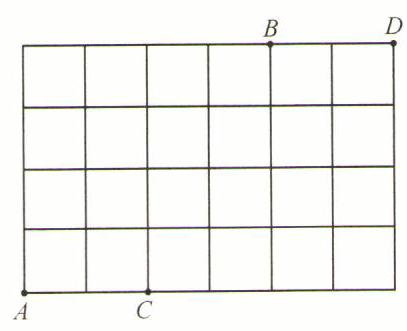
\includegraphics[width=0.3\textwidth]{bodyxb/src/bo_d1ig044601uc738hj6v0_141_1076_1728_407_331_0.jpg}
\end{center}

第 3 题图

3. 如图所示,甲、乙两人同时出发,甲从点 $A$ 到 $B$ ,乙从点 $C$ 到 $D$ ,且每人每次都只能向上或向右走一格,则甲、乙的行走路线没有公共点的概率为(   ).

A. $\dfrac{3}{7}$ B. $\dfrac{5}{7}$ C. $\dfrac{5}{14}$ D. $\dfrac{13}{21}$

4. 如图,在平面直角坐标系 ${xOy}$ 中, $O$ 为正八边形 ${A}_{1}{A}_{2}\cdots {A}_{8}$ 的中心, ${A}_{1}\left( {1,0}\right)$ . 任取不同的两点 ${A}_{i}\text{ 、 }{A}_{j}$ ,点 $P$ 满足 $\vv{OP} +$  $\vv{O{A}_{i}} + \vv{O{A}_{j}} = \vv{0}$ ,则点 $P$ 落在第一象限的概率是\blkda{}.

\begin{center}
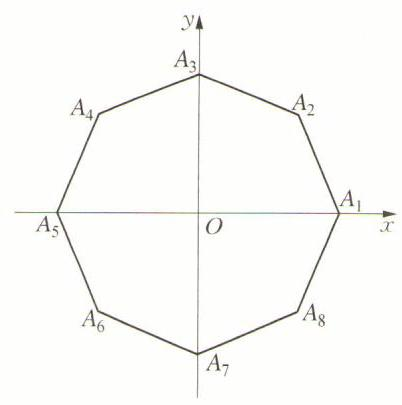
\includegraphics[width=0.3\textwidth]{bodyxb/src/bo_d1ig044601uc738hj6v0_142_1115_272_402_405_0.jpg}
\end{center}

第 4 题图

5. 对于函数 $f\left( x\right)$ ,其定义域为 $D$ ,若对任意的 ${x}_{1},{x}_{2} \in  D$ ,当 ${x}_{1} < {x}_{2}$ 时都有 $f\left( {x}_{1}\right)  \leq  f\left( {x}_{2}\right)$ ,则称函数 $f\left( x\right)$ 为 “不严格单调增函数”,若函数 $f\left( x\right)$ 定义域为 $D = \{ 1,2,3,4,5$ , $6\}$ ,值域为 $A = \{ 7,8,9\}$ ,则函数 $f\left( x\right)$ 是“不严格单调增函数”的概率是\blkda{}.

6. 概率论起源于赌博问题. 法国著名数学家布莱尔 · 帕斯卡遇到两个赌徒向他提出的赌金分配问题: 甲、乙两赌徒约定先赢满 5 局者,可获得全部赌金 700 法郎,当甲赢了 4 局,乙赢了 3 局,不再赌下去时,赌金如何分配？假设每局两人输赢的概率各占一半,每局输赢相互独立,那么赌金分配比较合理的是(   ).

A. 甲 525 法郎, 乙 175 法郎 B. 甲 500 法郎, 乙 200 法郎

C. 甲 400 法郎, 乙 300 法郎 D. 甲 350 法郎, 乙 350 法郎

7. 已知随机事件 $A\text{ 、 }B$ 发生的概率满足 $P\left( {A \cup  B}\right)  = {0.9}$ ,小华猜测事件 $\bar{A} \cap  \bar{B}$ 会发生,小明猜测事件 $\bar{A} \cap  \bar{B}$ 不会发生,则以下判断中正确的是\blkda{}. (请填写序号)

① 小华一定猜错；

② 小华和小明猜对的可能性一样大；

③ 小明猜对的可能性更大;

④ 无法判断小华和小明谁猜对的可能性更大.

8. 已知事件 $\bar{A}$ 与 $\bar{B}$ 互斥,事件 $A\text{ 、 }B$ 同时发生的概率为 $\dfrac{2}{5}$ ,且 $P\left( \bar{A}\right)  = {2P}\left( \bar{B}\right)$ ,则 $P\left( A\right)  =$ \blkda{}.

9. 在嘉年华游戏中, $A\text{ 、 }B$ 两人轮流抛掷同一枚质地不均匀的硬币,已知硬币正面朝上的概率是 $\dfrac{2}{3}$ ,反面朝上的概率是 $\dfrac{1}{3}$ ,抛掷规则如下: 如果掷出正面,则下一次由同一个人继续抛掷; 如果掷出反面,则下一次由另一个人抛掷,第一次由 $A$ 抛掷,则第 $n$ 次是 $A$ 抛掷的概率是\blkda{}.

10. 在发生某公共卫生事件期间,有专业机构认为该事件在一段时间没有发生大规模群体感染的标志为 “连续 10 天,每天新增疑似病例不超过 7 人”. 根据过去 10 天甲、乙、丙、丁四地新增疑似病例数据,一定符合该标志的是(   ).

A. 甲地:均值为 3 ,中位数为 4

B. 乙地:均值为 1 , 方差大于 0

C. 丙地:中位数为 2 , 众数为 3

D. 丁地:均值为 2 ,方差为 3

11. 某果园种植了一批苹果树,分为 $A\text{ 、 }B$ 两个品种,为调查苹果产量 (单位: ${{kg}}$ ),采用分层随机抽样原则抽取了 20 个样本. 现由于某种原因,这些原始样本数据不可查得,已知样本中 $A$ 品种 12 棵,平均产量为 30,方差为 14; $B$ 品种 8 棵,平均产量为 35,方差为 10,则利用已知数据可估计出这批苹果树产量的总体方差为\blkda{}.